% !TeX program = xelatex
% A题完整论文（四问）：基于仓库 results/problem1_improved、problem2_fvm_bdf、problem3_fvm_bdf、problem4_fvm_bdf 与对应 code/ 目录整理；前三问承接 agent_B 初稿，问题四（移动边界·半径收缩·附录4）由 agent_A 补全。
\documentclass[UTF8,a4paper,12pt]{ctexart}

\usepackage[left=2.54cm,right=2.54cm,top=2.54cm,bottom=2.54cm]{geometry}
\usepackage{amsmath,amssymb,mathtools,bm}
\usepackage{booktabs,longtable,array,multirow,tabularx}
\usepackage{graphicx,float,subcaption}
\usepackage{caption}
\usepackage{xcolor}
\usepackage{enumitem}
\usepackage{listings}
\usepackage{hyperref}
\usepackage{titlesec}
\usepackage{fancyhdr}
\usepackage{indentfirst}

\IfFontExistsTF{SimSun}{\setCJKmainfont[AutoFakeBold=2]{SimSun}}{}
\IfFontExistsTF{Times New Roman}{\setmainfont{Times New Roman}}{}
\linespread{1.0}\selectfont
\setlength{\parindent}{2em}
\setlength{\parskip}{0pt}
\setlength{\emergencystretch}{2em}
\setcounter{secnumdepth}{3}
\setcounter{tocdepth}{2}
\renewcommand{\theequation}{\arabic{equation}}

\captionsetup{font={small},labelfont=bf,labelsep=quad,skip=2pt,aboveskip=2pt,belowskip=0pt}
\setlength{\abovecaptionskip}{2pt}
\setlength{\belowcaptionskip}{0pt}
\setlength{\floatsep}{4pt plus 1pt minus 1pt}
\setlength{\textfloatsep}{4pt plus 1pt minus 1pt}
\setlength{\intextsep}{4pt plus 1pt minus 1pt}

\ctexset{
  section={format=\centering\bfseries\fontsize{14pt}{18pt}\selectfont, name={,、}, number=\chinese{section}, aftername=\quad, beforeskip=14pt, afterskip=8pt},
  subsection={format=\bfseries\fontsize{12pt}{16pt}\selectfont, beforeskip=10pt, afterskip=5pt},
  subsubsection={format=\bfseries\fontsize{12pt}{16pt}\selectfont, beforeskip=8pt, afterskip=4pt}
}
\pagestyle{fancy}
\fancyhf{}
\cfoot{\thepage}
\renewcommand{\headrulewidth}{0pt}

\lstset{basicstyle=\ttfamily\small,breaklines=true,frame=single,columns=fullflexible,numbers=left,numberstyle=\tiny,showstringspaces=false}
\hypersetup{colorlinks=true,linkcolor=black,citecolor=black,urlcolor=black,pdftitle={药材热风烘干过程的热质耦合建模与数值模拟}}

\begin{document}

\begin{center}
  {\fontsize{14pt}{18pt}\selectfont\bfseries 药材热风烘干过程的热质耦合建模与数值模拟}\par\vspace{10pt}
  {\fontsize{14pt}{18pt}\selectfont\bfseries 摘要}
\end{center}

热风烘干是中药材加工的重要环节，烘房环境通过药材表面向内部传热，同时推动内部水分向外迁移。为描述这一过程，本文根据药材细长圆柱的形状特征，忽略轴向传递和端面影响，建立一维轴对称径向传热传质模型。烘房温度与水分浓度由附件数据插值得到，药材表面采用换热、传质边界。四个问题依次考虑常物性预热、变物性热湿耦合、固定半径下的干燥达标以及半径收缩后的干燥达标，空间上统一采用圆柱径向有限体积法，时间上采用自适应 BDF 方法，从而在同一框架内逐步加入物性变化、终止判据和移动边界。

针对问题一，首先将附件1中的离散环境数据处理为随时间连续变化的边界条件，再根据附录2的常物性关系分别建立 Fourier 径向导热方程和 Fick 径向扩散方程。由于水分扩散系数不含温度项，温度场与水分场可以分开求解。利用有限体积法处理圆柱中心和表面边界后，得到预热阶段各时刻、各半径位置的温度和水分浓度，并将完整结果保存至 \texttt{result1.xlsx}。在 $1800\rm\,s$ 时，中心与表面温度分别为 \textbf{\boldmath$33.5753^\circ\mathrm C$、$36.7856^\circ\mathrm C$}，中心与表面水分浓度分别为 \textbf{\boldmath$2.5500\rm\,kg/kg$、$1.5102\rm\,kg/kg$}。温度变化已传入内部，而水分下降主要集中在近表面区域，说明预热阶段的传热速度快于内部水分扩散。

针对问题二，附录3中的密度、比热容和热导率随水分变化，水分扩散系数又同时受温度与水分影响。为反映这种相互作用，本文将温度场和水分场合并为联合状态，建立变物性的热湿耦合模型，并在每个时间步同步更新物性和界面通量。由此得到整个烘干过程前三小时的温度、水分分布，完整结果保存至 \texttt{result2.xlsx}。在 $3\rm\,h$ 时，中心与表面温度分别为 \textbf{\boldmath$49.8495^\circ\mathrm C$、$49.9664^\circ\mathrm C$}，中心与表面水分浓度分别为 \textbf{\boldmath$1.7662\rm\,kg/kg$、$1.0081\rm\,kg/kg$}。此时温度已接近均匀，水分仍保持明显的径向梯度，表明恒温干燥后期主要受内部水分迁移限制。

针对问题三，仍采用固定半径热湿耦合模型，并从烘干初始状态重新计算。题目要求药材各处水分浓度均低于规定阈值，因此本文以全截面最大水分浓度构造终止事件，通过连续事件搜索确定首次达标时间，而不以表面值或平均值代替。附件1结束后的烘房条件采用末值延续，并用不同边界情景检验这一假设的影响；同时采用另一种隐式方法进行交叉验证。计算得到连续达标时间为 \textbf{\boldmath$t^*=205821.7420\rm\,s=57.1727\rm\,h$}，第一个满足要求的 $60\rm\,s$ 输出时刻为 \textbf{\boldmath$57.1833\rm\,h$}，完整水分结果保存至 \texttt{result3.xlsx}。终止时全域最大水分位于中心，说明药材中心的干燥滞后决定了最终停机时刻；边界扰动下的达标时间范围为 \textbf{\boldmath$53.6154$--$61.0702\rm\,h$}。

针对问题四，在问题三的达标判据上进一步引入附件2给出的半径变化，并采用附录4的物性关系。本文利用 Landau 变换将随时间收缩的物理区域映射到固定计算区域，以无量纲物质坐标标记药材内部位置，再根据当前半径更新传热传质尺度，实现收缩条件下温度场和水分场的同步求解。计算得到连续达标时间为 \textbf{\boldmath$t^*=182968.2250\rm\,s=50.8245\rm\,h$}，第一个满足要求的 $60\rm\,s$ 输出时刻为 \textbf{\boldmath$50.8333\rm\,h$}，完整水分结果保存至 \texttt{result4.xlsx}。与问题三相比，达标时间缩短约 \textbf{\boldmath$6.35\rm\,h$}；边界扰动下的终止时间范围为 \textbf{\boldmath$47.6834$--$54.2753\rm\,h$}。结果表明，在题给半径轨迹和物性关系下，尺寸收缩缩短了水分迁移路径，使药材更早达到干燥要求。

\noindent \textbf{关键词}：药材热风干燥\quad 热质耦合\quad 有限体积法\quad 向后微分公式\quad Landau变换

\newpage
\section{问题重述}
\subsection{问题背景}
热风烘干是中药材加工中的常见工序。烘干不足时，药材内部残余水分偏高，不利于后续贮藏；烘干过度时，又会增加能耗，并可能影响药材品质。因此，如何根据药材内部温度和水分分布判断烘干进程，是本题需要解决的核心问题。

从物理过程看，热风首先作用于药材表面，表面温度和含水率变化较快；中心区域只能依靠内部导热和水分扩散逐步响应，通常存在明显滞后。若后期药材发生收缩，半径减小又会改变扩散距离和空间边界。由此可知，仅根据表面含水率或平均含水率判断停机时间并不充分，必须建立能够描述径向分布的传热传质模型。

题目将药材近似为长 $25\rm\,cm$、初始半径 $2\rm\,cm$ 的圆柱体，给定初始温度、初始干基含水率、烘房温湿度数据以及不同阶段的物性经验式；附件2还给出了半径随时间变化的数据。本文据此把药材内部过程简化为一维径向问题，按常物性、变物性、固定半径达标和收缩半径达标四个层次建立模型，逐步分析物性变化、边界外推和半径收缩对计算结果的影响。

\subsection{问题提出}
四个问题的建模要求具有递进关系，可整理为以下任务。

\textbf{问题一：}在 $0$ 到 $1800\rm\,s$ 的预热阶段内，基于附录2物性关系建立温度场和水分场模型，给出表\ref{tab:q1-temp}、表\ref{tab:q1-moist} 所需结果，并按 $1\rm\,s$ 时间分辨率和 $0.1\rm\,cm$ 径向分辨率输出完整数据。

\textbf{问题二：}在固定半径条件下，将物性关系改为附录3经验式，建立温度与水分相互影响的热湿耦合模型，给出前 $3\rm\,h$ 内每隔 $0.5\rm\,h$、半径 $0,0.5,1,1.5,2\rm\,cm$ 处的温度和水分浓度。

\textbf{问题三：}沿用问题二的固定半径耦合模型，继续计算至药材各处水分浓度均低于 $0.15\rm\,kg/kg$，确定达标烘干时间，并输出每隔 $6\rm\,h$ 以及终止时刻的水分浓度分布。

\textbf{问题四：}在问题三的达标判据基础上引入附件2给出的半径收缩轨迹 $R(t)$，同时将物性关系改为附录4，求移动边界条件下药材全截面水分浓度达标所需时间，并输出每隔 $6\rm\,h$ 以及终止时刻、含移动表面位置的数据。

\section{问题分析}
四个问题均围绕圆柱药材内部的径向传热、传质展开，区别主要体现在物性关系、计算时长和几何边界三个方面。问题一是常物性预热阶段，用于确定空间离散、表面边界和输出插值方法；问题二引入状态相关物性，需要同步推进温度场和水分场；问题三在固定半径下延长计算时间，重点转为达标判据和边界外推；问题四进一步考虑半径收缩，将固定区域问题变为移动边界问题。因此，本文不把四问割裂处理，而是在同一径向守恒框架上逐层加入新的物理因素。

\subsection{问题一分析}
问题一只计算 $0$ 到 $1800\rm\,s$ 的预热过程，该时间段完全处在附件1给出的烘房边界范围内。附录2中密度、比热容和热导率均为常数，水分扩散系数只与水分浓度有关，不含温度项，因此温度方程和水分方程在本问中可以分别求解。该问的关键不是寻找停机时刻，而是建立可靠的径向控制体格式、第三类边界处理和结果输出方法，并观察表面快速响应与中心滞后之间的差异。

\subsection{问题二分析}
问题二仍采用固定半径和相同类型的表面边界，但物性关系由附录2改为附录3。此时 $\rho,c_p,k$ 随水分浓度变化，$D$ 同时依赖水分浓度和绝对温度。也就是说，温度会影响水分扩散速率，水分变化又会通过物性参数影响能量方程。若先求温度再代入水分方程，容易在非线性物性上产生时间滞后。因此，本问应把温度和水分作为联合状态同步积分，并沿用问题一建立的径向守恒离散结构。

\subsection{问题三分析}
问题三把问题二的固定半径耦合模型从前三小时延长到烘干终点。题目要求药材“各处”水分浓度均低于 $0.15\rm\,kg/kg$，因此终止判据必须作用于全截面的最大水分浓度。若只检查表面值或平均值，将会提前停机，无法反映中心区域的干燥滞后。该问还涉及边界外推：附件1只覆盖前 $4\rm\,h$，而达标时间预计远超过 $4\rm\,h$，因此需要给出后续烘房工况假设，并在结果中区分数值误差与边界假设造成的不确定性。

\subsection{问题四分析}
问题四在问题二、问题三的基础上同时改变物性和几何边界。附录4给出新的物性经验式，附件2给出随时间减小的半径 $R(t)$，计算区域由固定区间 $[0,R]$ 变为移动区间 $[0,R(t)]$。若直接在物理半径上计算，每个时间步都需要处理移动网格，数值实现较繁琐。为此，可引入 $\xi=r/R(t)$，把移动区域映射到固定区间 $[0,1]$。在均匀径向收缩假设下，$\xi$ 可视为同一物质层的位置标签，半径变化主要通过扩散尺度项影响水分迁移。题给半径轨迹与附录4密度经验式是否完全满足干物质守恒，将在模型检验部分进一步讨论。

综合上述分析，四个问题并非相互独立，而是在统一径向传热传质框架下逐步增加物性非线性、终点判据与移动边界效应。本文按照“预热平衡—热质耦合—终点判定—移动边界”的递进思路展开建模，并在各阶段采用与模型复杂度相适应的数值方法。整体建模与求解技术路线如图\ref{fig:overall-route}所示。

\begin{figure}[H]
  \centering
  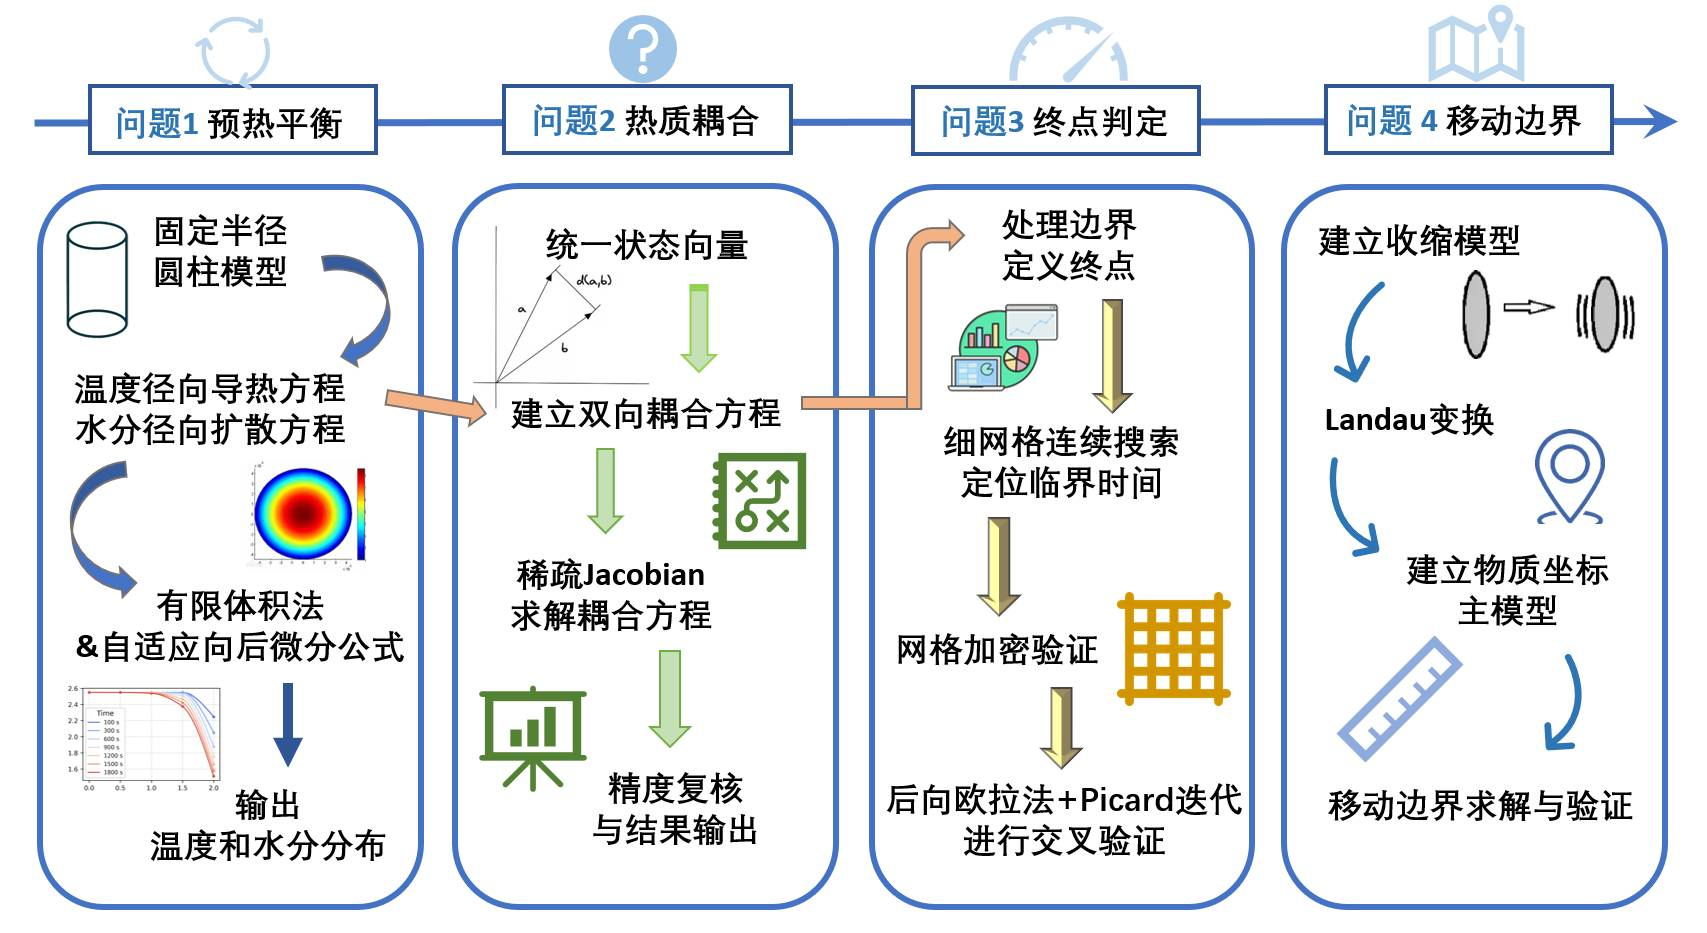
\includegraphics[width=\textwidth]{figures/overall_route.jpg}
  \caption{四个问题的递进式建模与求解技术路线}
  \label{fig:overall-route}
\end{figure}

如图\ref{fig:overall-route}所示，问题一首先在固定半径和常物性条件下建立径向传热、传质模型，为后续计算提供基础；问题二进一步引入状态相关物性，将温度场与水分场统一为耦合状态进行求解；问题三在热湿耦合模型基础上引入全截面含水率终止判据，通过连续搜索确定临界干燥时间；问题四进一步考虑药材半径随时间收缩的移动边界，通过坐标变换将变区域问题转化为固定计算域上的耦合问题。由此形成由基础物理场模拟向实际停机判定逐级推进的完整建模体系。

\section{模型假设}
\begin{enumerate}[label=\arabic*.,leftmargin=2.5em]
  \item 药材近似为轴对称长圆柱体。由于长度明显大于半径，忽略轴向传递和端面效应，只考虑径向一维传热、传质过程。
  \item 初始时刻药材内部状态均匀，$T(r,0)$ 与 $C(r,0)$ 均不随半径变化；烘房环境视为空间均匀混合。
  \item 题目未给出显式蒸发潜热源项所需参数，本文在题设经验物性体系内建模，不额外加入相变潜热源项。
  \item 问题四采用前置固定变换处理移动边界，认为半径收缩为均匀径向缩放。
\end{enumerate}

\section{符号说明}
\begin{table}[H]
  \centering
  \caption{主要符号说明}
  \label{tab:symbols}
  \begin{tabular}{>{\centering\arraybackslash}p{0.18\textwidth}p{0.55\textwidth}>{\centering\arraybackslash}p{0.17\textwidth}}
    \toprule
    符号 & 含义 & 单位\\ \midrule
    $r$ & 到药材中心轴的径向距离 & m\\
    $R,\ R(t)$ & 药材半径；前三问取常数 $0.02\rm\,m$，问题四为随时间变化的半径 & m\\
    $\xi$ & 问题四采用的物质坐标，$\xi=r/R(t)\in[0,1]$ & 无量纲\\
    $t$ & 烘干时间 & s\\
    $T(r,t)$ & 药材内部温度 & $^\circ\mathrm C$\\
    $T_K$ & 绝对温度，$T_K=T+273.15$ & K\\
    $C(r,t)$ & 干基水分浓度 & kg/kg\\
    $T_\infty(t)$ & 烘房环境温度 & $^\circ\mathrm C$\\
    $C_\infty(t)$ & 烘房环境水分浓度 & kg/kg\\
    $\rho(C)$ & 密度 & kg/m$^3$\\
    $c_p(C)$ & 比热容 & J/(kg$\cdot$K)\\
    $k(C)$ & 热导率 & W/(m$\cdot$K)\\
    $D(C,T_K)$ & 有效水分扩散系数 & m$^2$/s\\
    $h$ & 对流换热系数 & W/(m$^2\cdot$K)\\
    $h_m$ & 对流传质系数 & m/s\\
    $N$ & 径向离散节点数 & 无量纲\\
    $\Delta r$ & 固定半径模型中的径向网格尺度 & m\\
    $\Delta t$ & 输出或时间推进步长 & s\\
    $g(t)$ & 终止事件函数，$g(t)=\max C-0.15$ & kg/kg\\
    $t^*$ & 达到水分阈值所需烘干时间，即连续事件定位的临界时刻 & h\\
    \bottomrule
  \end{tabular}
\end{table}

\section{模型准备}
四个问题在物性关系、计算时长和半径条件上逐步变化，但数据调用和空间离散可以统一处理。本节先说明附件中离散时间序列的插值与外推方式，再给出采用一维径向模型的依据，最后建立后续各问共同使用的有限体积离散格式。这样处理可以保证四问之间只改变必要的物理条件，而不因离散方法变化引入额外误差。

\subsection{边界数据插值}
附件1只给出了若干离散时刻的烘房温度和环境水分浓度，而隐式时间积分器会在自适应时间步上反复调用边界值。因此，需先将附件数据扩展为连续时间函数。本文对烘房温度 $T_\infty(t)$ 和环境水分浓度 $C_\infty(t)$ 均采用分段线性插值：
\begin{equation}
  y_\infty(t)=y_j+\frac{y_{j+1}-y_j}{t_{j+1}-t_j}(t-t_j),
  \qquad t_j\le t\le t_{j+1},
\end{equation}
其中 $y$ 可表示温度或水分浓度。问题一和问题二的报告时段均在附件1覆盖范围内，边界值直接由上述插值式给出。问题三、问题四需要继续计算到水分达标，计算时间可能超过 $4\rm\,h$，超出附件1范围后采用末值保持：
\begin{equation}
  T_\infty(t)=T_\infty(4{\rm h}),\qquad C_\infty(t)=C_\infty(4{\rm h}),\qquad t>4{\rm h}.
\end{equation}
这一处理等价于假定 $4\rm\,h$ 后烘房进入稳定运行阶段。由于该假设会直接影响后期干燥速率，本文在模型检验中另设边界扰动情景，用于衡量外推方式对达标时间的影响。

\subsection{半径收缩数据插值}
问题四需要考虑药材半径随时间收缩，因此必须在积分过程中实时更新 $R(t)$。附件2给出了离散时刻的半径数据，本文仍采用分段线性插值：
\begin{equation}
  R(t)=R_j+\frac{R_{j+1}-R_j}{t_{j+1}-t_j}(t-t_j),
  \qquad t_j\le t\le t_{j+1},
\end{equation}
附件2覆盖 $0$ 到 $72\rm\,h$，采样间隔为 $1800\rm\,s$，半径由 $2.0\rm\,cm$ 单调减小到 $1.198\rm\,cm$。若计算时间超过 $72\rm\,h$，半径取附件末值；本文问题四得到的终止时间小于 $72\rm\,h$，实际计算中没有触发该外推。需要说明的是，$R(t)$ 在本文中作为题目给定的经验轨迹使用，不再由质量守恒方程反求。

\subsection{几何简化依据}
将圆柱药材简化为一维径向模型，需要同时满足两个判断：一是内部温度和水分梯度不能忽略，二是端面效应相对较弱。前者可用热 Biot 数和质 Biot 数估计：
\begin{equation}
  Bi_T=\frac{hR}{k},\qquad Bi_C=\frac{h_mR}{D(C_0)}.
\end{equation}
按问题一参数估计，$Bi_T\approx1.389$、$Bi_C\approx3.24$，均大于 $0.1$。这说明药材内部存在明显梯度，不能用集总参数模型代替空间分布模型。另一方面，$1800\rm\,s$ 内热扩散尺度和水分扩散尺度分别为
\begin{equation}
  l_T=\sqrt{\alpha t},\qquad l_C=\sqrt{D(C_0)t},\qquad \alpha=\frac{k}{\rho c_p}.
\end{equation}
代入参数可得 $l_T\approx1.74\rm\,cm$、$l_C\approx0.30\rm\,cm$，均小于圆柱半长 $12.5\rm\,cm$。因此，在题目给定的主要计算尺度内，端面影响不会主导整体干燥过程，忽略轴向传递是合理的。

\subsection{径向有限体积离散}
柱坐标方程中含有 $1/r$ 项，若直接差分，中心点和表面通量处理容易不一致。为保持守恒结构，本文采用有限体积法。取单位长度圆柱截面，节点 $r_i=i\Delta r$，控制体体积和界面面积分别为
\begin{equation}
  V_i=\pi\left(r_{i+1/2}^2-r_{i-1/2}^2\right),\qquad
  A_{i+1/2}=2\pi r_{i+1/2}.
\end{equation}
对具有径向扩散形式的一般方程
\begin{equation}
  a(u)\frac{\partial u}{\partial t}
  =\frac1r\frac{\partial}{\partial r}\left(r\,b(u)\frac{\partial u}{\partial r}\right),
\end{equation}
在每个控制体上积分并用相邻节点差商表示界面通量，可得内部节点的半离散形式：
\begin{equation}
  a_iV_i\frac{du_i}{dt}
  =b_{i-1/2}A_{i-1/2}\frac{u_{i-1}-u_i}{\Delta r}
  +b_{i+1/2}A_{i+1/2}\frac{u_{i+1}-u_i}{\Delta r}.
\end{equation}
其中 $a(u)$ 对应热容项或水分储存项，$b(u)$ 对应热导率或水分扩散系数。中心处因界面面积为零，自然满足对称零通量条件；表面控制体则在扩散通量之外加入对流换热或传质通量，从而实现第三类边界。后续各问只需替换物性函数、边界函数以及是否引入 $R(t)$，空间离散框架保持不变。

\section{问题一模型的建立与求解}
\subsection{本问任务与前文承接}
问题一研究固定半径、常物性条件下的预热过程，计算时间为 $0$ 到 $1800\rm\,s$。该问采用附录2物性关系，温度方程和水分方程尚未形成双向耦合，因此可作为全文数值框架的基准算例。本文先通过本问确定径向有限体积离散、第三类边界和指定位置输出方法，后续问题再在同一框架上加入变物性、达标事件函数和移动边界。

\subsection{模型建立}
在固定半径 $R=0.02\rm\,m$ 内，药材温度场满足径向 Fourier 热传导方程：
\begin{equation}
  \rho c_p\frac{\partial T}{\partial t}
  =\frac1r\frac{\partial}{\partial r}
  \left(kr\frac{\partial T}{\partial r}\right),
  \qquad 0<r<R.
\end{equation}
水分场满足径向 Fick 扩散方程：
\begin{equation}
  \frac{\partial C}{\partial t}
  =\frac1r\frac{\partial}{\partial r}
  \left[rD(C)\frac{\partial C}{\partial r}\right],
  \qquad
  D(C)=7\times10^{-9}\exp\left(-\frac{0.89}{C}\right).
\end{equation}
初始条件为
\begin{equation}
  T(r,0)=28,\qquad C(r,0)=2.55.
\end{equation}
中心对称边界为
\begin{equation}
  \left.\frac{\partial T}{\partial r}\right|_{r=0}=0,\qquad
  \left.\frac{\partial C}{\partial r}\right|_{r=0}=0.
\end{equation}
表面 Robin 边界为
\begin{equation}
  -k\left.\frac{\partial T}{\partial r}\right|_{r=R}
  =h\left[T(R,t)-T_\infty(t)\right],
\end{equation}
\begin{equation}
  -D(C_s)\left.\frac{\partial C}{\partial r}\right|_{r=R}
  =h_m\left[C(R,t)-C_\infty(t)\right].
\end{equation}
上述两个表面条件分别描述药材表面与热风之间的换热和换质。由于本问中 $\rho,c_p,k$ 为常数，且 $D(C)$ 不含温度项，温度场与水分场之间没有直接耦合，可以分别积分求解。

\subsection{模型求解}
空间方向采用前文建立的径向有限体积格式，时间方向采用自适应 BDF 隐式积分。计算以几何半径 $R$、初值 $T_0,C_0$、附件1边界序列和附录2物性参数为已知条件，先对烘房温度和环境水分浓度建立线性插值函数，再分别组装温度方程和水分方程的右端项，积分至 $1800\rm\,s$ 后抽取题目指定时间和半径位置的结果。

内部计算网格取 $\Delta r=0.0025\rm\,cm$，使表面附近的温度和水分梯度能够被充分分辨；得到连续半径网格上的数值解后，再抽取到题目要求的 $0.1\rm\,cm$ 输出位置。水分扩散系数 $D(C)$ 随含水率变化较快，界面扩散系数采用调和平均，以避免在低扩散区域高估界面通量。

输出前设置 $C\leftarrow\max(C,0)$ 作为非负保护。

\subsection{结果分析}
表\ref{tab:q1-temp} 和表\ref{tab:q1-moist} 给出了问题一的代表性输出。温度场在半小时内整体升高，并由表面向中心逐步传递。$1800\rm\,s$ 时，表面温度为 $36.7856^\circ\mathrm C$，中心温度为 $33.5753^\circ\mathrm C$，说明热量已进入药材内部，但径向温差仍然存在。水分场的响应慢于温度场：同一时刻表面含水率降至 $1.5102\rm\,kg/kg$，中心仍保持 $2.5500\rm\,kg/kg$，脱水主要集中在近表面区域。

\begin{table}[H]
  \centering
  \caption{30分钟内药材的温度 $/^\circ\mathrm C$}
  \label{tab:q1-temp}
  \begin{tabular}{rrrrrr}
    \toprule
    时间/s & 0 cm & 0.5 cm & 1 cm & 1.5 cm & 2 cm\\ \midrule
    100 & 28.0001 & 28.0003 & 28.0040 & 28.0327 & 28.1801\\
    300 & 28.0408 & 28.0635 & 28.1514 & 28.3681 & 28.8489\\
    600 & 28.4533 & 28.5360 & 28.8039 & 29.3159 & 30.1652\\
    900 & 29.3243 & 29.4583 & 29.8755 & 30.6161 & 31.7304\\
    1200 & 30.5427 & 30.7098 & 31.2223 & 32.1126 & 33.4276\\
    1500 & 31.9957 & 32.1867 & 32.7660 & 33.7463 & 35.1203\\
    1800 & 33.5753 & 33.7720 & 34.3642 & 35.3621 & 36.7856\\
    \bottomrule
  \end{tabular}
\end{table}

\begin{table}[H]
  \centering
  \caption{30分钟内药材的水分浓度 $/\rm kg\cdot kg^{-1}$}
  \label{tab:q1-moist}
  \begin{tabular}{rrrrrr}
    \toprule
    时间/s & 0 cm & 0.5 cm & 1 cm & 1.5 cm & 2 cm\\ \midrule
    100 & 2.5500 & 2.5500 & 2.5500 & 2.5500 & 2.2471\\
    300 & 2.5500 & 2.5500 & 2.5500 & 2.5492 & 2.0508\\
    600 & 2.5500 & 2.5500 & 2.5500 & 2.5353 & 1.8770\\
    900 & 2.5500 & 2.5500 & 2.5497 & 2.5045 & 1.7547\\
    1200 & 2.5500 & 2.5500 & 2.5482 & 2.4646 & 1.6586\\
    1500 & 2.5500 & 2.5499 & 2.5445 & 2.4206 & 1.5787\\
    1800 & 2.5500 & 2.5497 & 2.5383 & 2.3755 & 1.5102\\
    \bottomrule
  \end{tabular}
\end{table}

\begin{figure}[H]
  \centering
  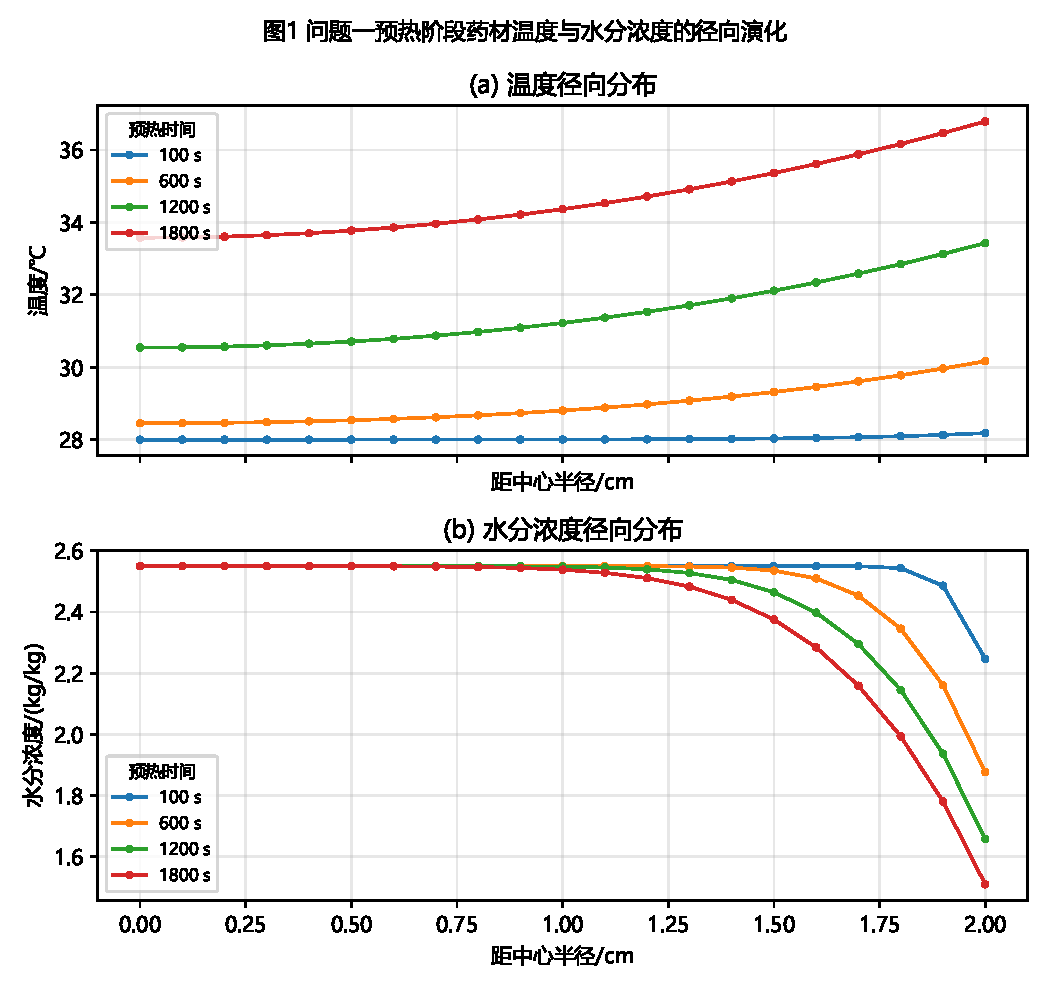
\includegraphics[width=0.88\textwidth]{figures/fig1_problem1_radial.pdf}
  \caption{问题一预热阶段药材温度与水分浓度的径向演化。(a) $100\rm\,s$、$600\rm\,s$、$1200\rm\,s$ 与 $1800\rm\,s$ 的温度径向分布；(b) 对应时刻的水分浓度径向分布。}
  \label{fig:q1-radial}
\end{figure}

由图\ref{fig:q1-radial}可见，各时刻温度均由中心向表面升高，且温度曲线随时间整体上移；水分浓度的明显下降则主要集中在近表面区域，中心在 $1800\rm\,s$ 内基本保持初值。两类剖面的差异说明，预热阶段的热量传递快于内部水分扩散，这也为后续将干燥过程的控制环节归结为内部传质提供了依据。

\begin{figure}[H]
  \centering
  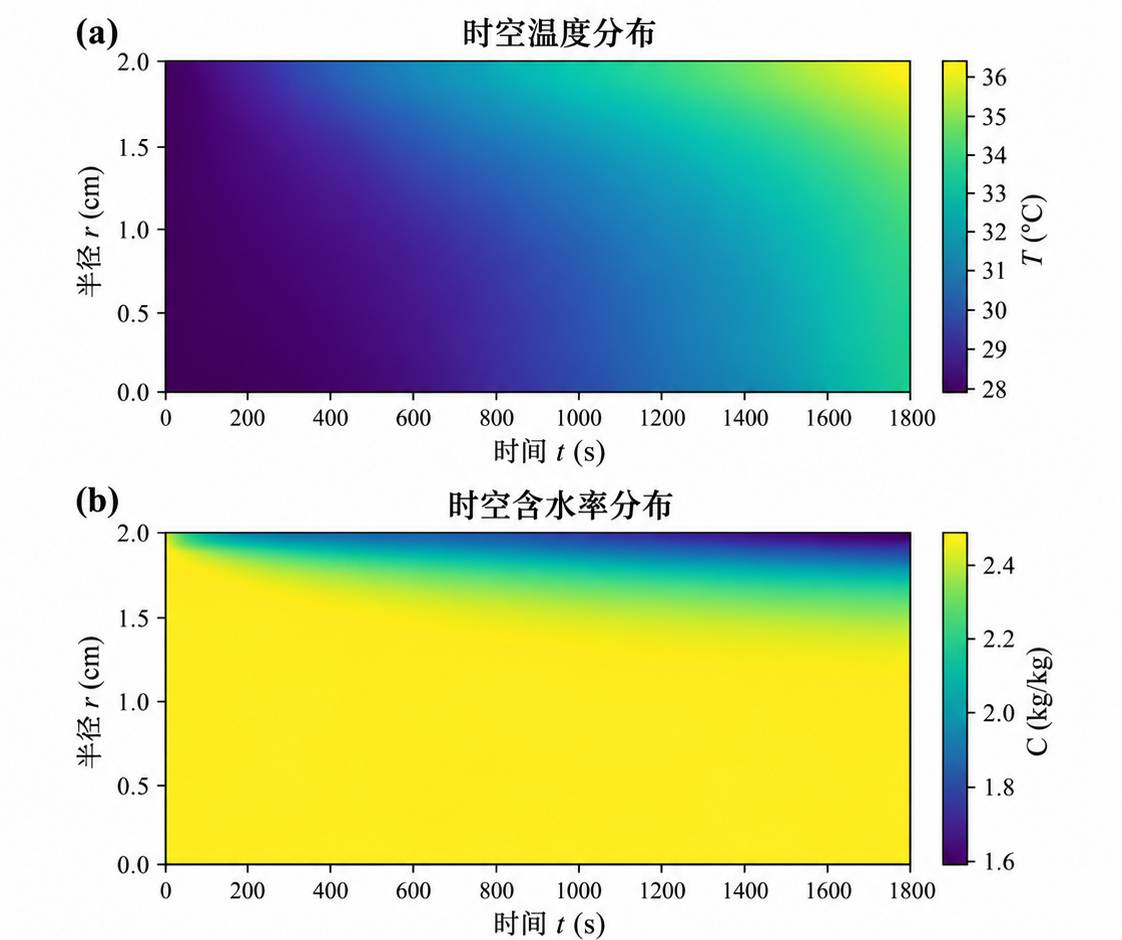
\includegraphics[width=0.75\textwidth]{figures/insert_1_cn.jpg}
  \caption{预热平衡阶段（$0$--$1800\rm\,s$）药材内部温度场与含水率场沿径向位置的时空演化特征。子图 (a) 展示温度分布，子图 (b) 展示含水率分布。}
  \label{fig:temp_moisture_heatmap}
\end{figure}

图\ref{fig:temp_moisture_heatmap} 用二维时空热图展示了预热阶段药材内部热湿状态的演化。可以看出，表层区域首先升温，随后热量向中心传递，形成由表面到中心递减的温度梯度；含水率则先在外层下降，并逐渐向内部推进。上述现象与第三类边界条件下的物理过程一致：外部热风先作用于表面，内部传递速度受有限热扩散和水分扩散限制。该结果说明本文的一维轴对称模型能够刻画预热阶段的主要热湿迁移特征。

\subsection{本问小结与后续衔接}
问题一表明，即使在常物性预热阶段，药材内部也已形成不可忽略的径向梯度，后续模型不能采用整体均匀近似。由本问确定的几何处理、第三类边界和守恒型径向离散将直接用于问题二；区别在于问题二的物性随状态变化，温度场和水分场需要作为联合系统同步求解。

\section{问题二模型的建立与求解}
\subsection{本问任务与前文承接}
问题二仍在固定半径圆柱区域内计算，但物性关系由附录2常物性改为附录3经验式，并要求给出 $0.5$--$3.0\rm\,h$ 内若干位置的温度和水分浓度。与问题一相比，本问的关键变化是温度场和水分场不再相互独立：水分浓度会改变密度、比热容和热导率，温度又通过绝对温度项影响水分扩散系数。因此，本问沿用问题一建立的径向有限体积空间离散，但在时间推进时将温度和水分合并为联合状态，同步求解热湿耦合系统。

\subsection{模型建立}
附录3给出的状态相关物性如下：
\begin{equation}
  \rho(C)=650+128C,
\end{equation}
\begin{equation}
  c_p(C)=1450+\frac{2736C}{C+1},
\end{equation}
\begin{equation}
  k(C)=0.21+\frac{0.38C}{C+1},
\end{equation}
\begin{equation}
  D(C,T)=2.4\times10^{-3}\exp\left(-\frac{0.45}{C}\right)
  \exp\left(-\frac{3850}{T_K}\right),\qquad T_K=T+273.15.
\end{equation}
在该物性体系下，能量方程写为
\begin{equation}
  \rho(C)c_p(C)\frac{\partial T}{\partial t}
  =\frac1r\frac{\partial}{\partial r}
  \left[rk(C)\frac{\partial T}{\partial r}\right].
\end{equation}
水分迁移仍采用守恒型径向扩散方程：
\begin{equation}
  \frac{\partial C}{\partial t}
  =\frac1r\frac{\partial}{\partial r}
  \left[rD(C,T)\frac{\partial C}{\partial r}\right].
\end{equation}
初始条件和中心对称边界沿用问题一。表面边界中的物性取表面状态值，写为
\begin{equation}
  -k(C_s)\left.\frac{\partial T}{\partial r}\right|_{r=R}
  =h\left[T(R,t)-T_\infty(t)\right],
\end{equation}
\begin{equation}
  -D(C_s,T_s)\left.\frac{\partial C}{\partial r}\right|_{r=R}
  =h_m\left[C(R,t)-C_\infty(t)\right].
\end{equation}

与问题一的常物性模型不同，问题二中材料热物性与传质物性均随当前状态发生变化。其中，水分浓度不仅直接决定密度、比热容和热导率，还与温度共同影响有效扩散系数。因此，温度场和水分场之间通过状态相关物性形成双向反馈，二者不能再视为相互独立的演化过程，其耦合关系如图\ref{fig:q2-coupling}所示。

\begin{figure}[H]
  \centering
  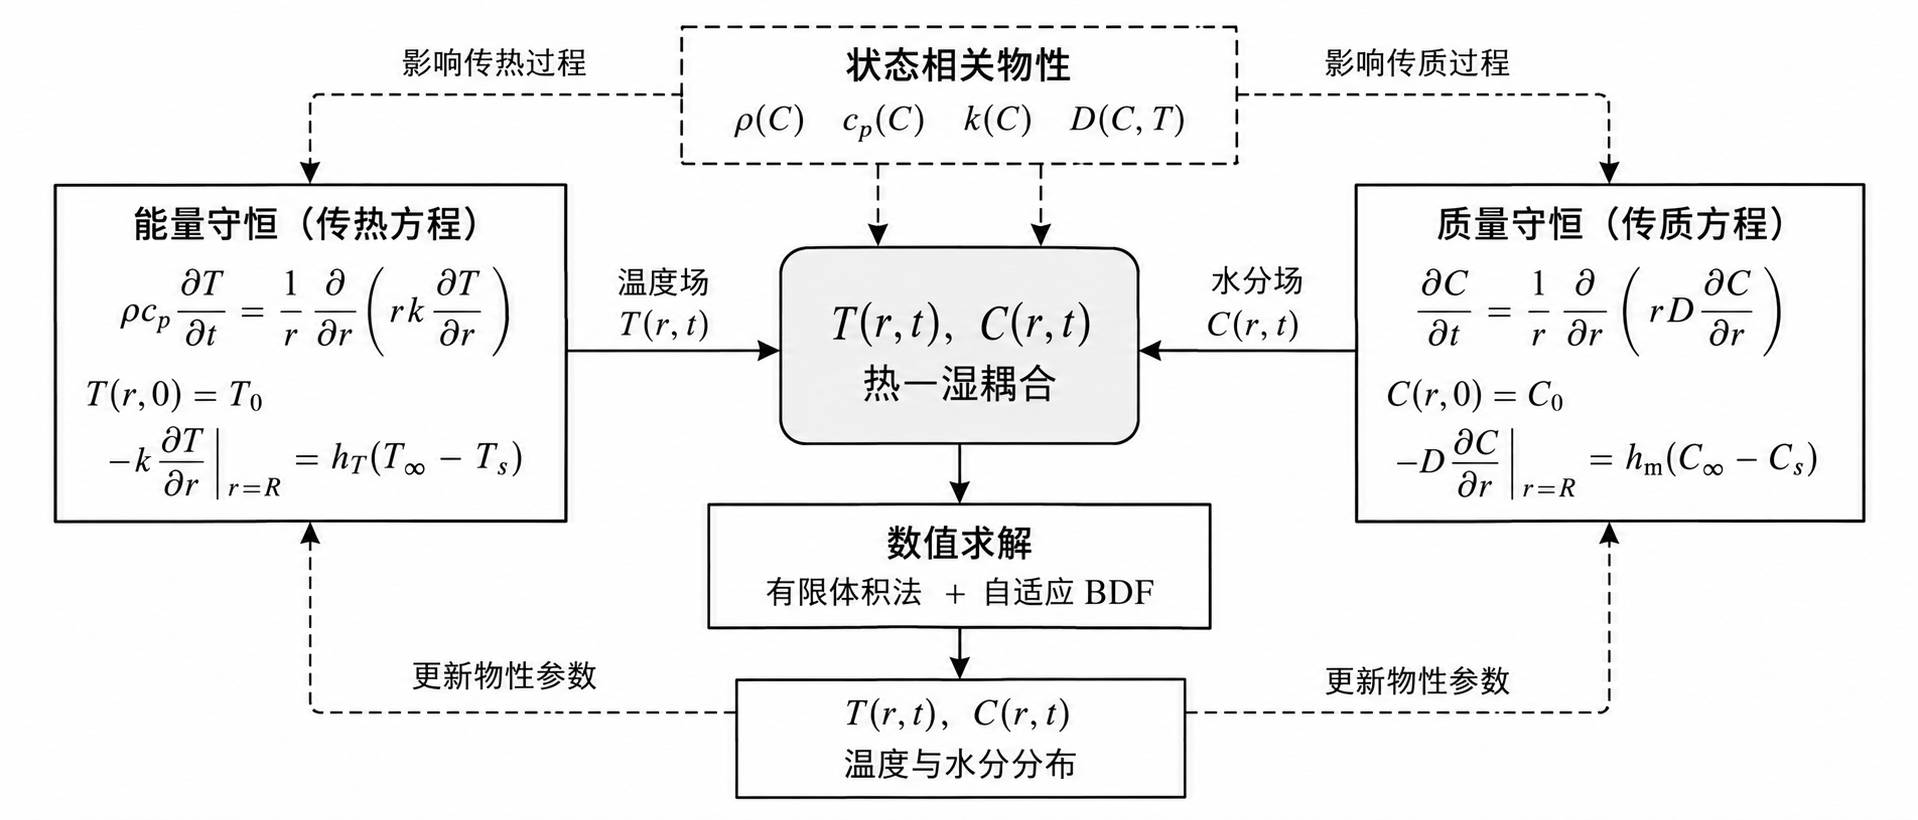
\includegraphics[width=\textwidth]{figures/coupling_mechanism.jpg}
  \caption{状态相关物性作用下的热湿双向耦合机制}
  \label{fig:q2-coupling}
\end{figure}

如图\ref{fig:q2-coupling}所示，能量守恒方程决定温度场 $T(r,t)$，质量守恒方程决定水分场 $C(r,t)$，二者又共同作用于状态相关物性参数。其中，$\rho(C)$、$c_p(C)$ 和 $k(C)$ 的变化反馈至传热过程，而 $D(C,T)$ 同时受温度和水分状态影响并反馈至传质过程，由此形成闭环热湿耦合系统。基于这一结构，本文将温度与水分拼接为统一状态向量，并在每个隐式时间步同步更新物性参数和两个物理场，避免“先求温度、再求水分”的分步计算引入额外滞后。

\subsection{模型求解}
问题二仍采用径向有限体积法进行空间离散。内部网格取 $\Delta r=0.025\rm\,cm$，共 81 个径向节点；温度和水分拼接后，联合状态维度为 162。控制体体积 $V_i=\pi(r_{i+1/2}^2-r_{i-1/2}^2)$、界面面积 $A_{i+1/2}=2\pi r_{i+1/2}$ 均按圆柱几何组装。界面热导率 $k$ 和扩散系数 $D$ 采用调和平均，以便在相邻控制体物性差异较大时保持通量计算稳定。

时间方向采用 \texttt{scipy.integrate.solve\_ivp} 中的自适应 BDF 隐式积分器。每次推进以上一时刻联合状态 $u^n=[T^n;C^n]$、附件1边界和附录3物性公式为基础，先计算 $\rho(C),c_p(C),k(C),D(C,T+273.15)$，再用调和平均得到界面 $k,D$。据此计算各控制体的传热、传质通量，并构成待求解方程。中心控制体自然满足对称零通量，表面控制体加入 Robin 对流通量，最终得到下一输出时刻联合状态 $u^{n+1}=[T^{n+1};C^{n+1}]$。

计算设置为 $\mathrm{rtol}=2\times10^{-8}$，温度和水分的绝对容差分别为 $2\times10^{-9}$、$2\times10^{-10}$，最大内部步长为 $5\rm\,s$。

由于 $T$ 与 $C$ 位于同一个状态向量内，BDF 在每个隐式步中同时处理热方程和水分方程的非线性残差，不再采用“先求温度、再求水分”的分步方式。为提高稳定性，非线性残差对应的块三对角稀疏 Jacobian 由解析式给出。

BDF 积分覆盖 $0$--$3\rm\,h$，并输出 10801 个 $1\rm\,s$ 时刻。内部最大步长受 $5\rm\,s$ 上限约束，最小步长出现在初期薄边界层。为检验数值稳定性，本文将网格由 $\Delta r=0.025\rm\,cm$ 加密至 $0.0125\rm\,cm$，在 30 个论文采样点上得到温度最大绝对差 $4.16\times10^{-5}\rm\,{}^\circ\mathrm C$、水分最大绝对差 $4.67\times10^{-5}\rm\,kg/kg$。进一步收紧 BDF 容差并缩小最大步长后，温度最大绝对差为 $1.91\times10^{-5}\rm\,{}^\circ\mathrm C$，水分最大绝对差为 $4.84\times10^{-8}\rm\,kg/kg$。这些差异均低于四位小数显示精度，说明表\ref{tab:q2-temp} 和表\ref{tab:q2-moist} 的结果对网格和时间容差不敏感。

\subsection{结果分析}
表\ref{tab:q2-temp} 和表\ref{tab:q2-moist} 给出了问题二的计算结果。药材温度在前 $2\rm\,h$ 上升较快，随后逐渐接近烘房温度；到 $3\rm\,h$ 时，中心温度为 $49.8495^\circ\mathrm C$，表面温度为 $49.9664^\circ\mathrm C$，二者仅相差约 $0.1169^\circ\mathrm C$。相比之下，水分浓度的径向差异仍然明显：$3\rm\,h$ 时中心为 $1.7662\rm\,kg/kg$，表面为 $1.0081\rm\,kg/kg$，中心与表面相差 $0.7581\rm\,kg/kg$。因此，恒温干燥后期的主要限制不再是升温，而是内部水分向表面的扩散。

图\ref{fig:q2-heatmap} 从时空角度展示了上述差异。温度等值线主要集中在前半段，随后逐渐稀疏，说明温度场较快趋于准均匀；水分等值线则在整个 $3\rm\,h$ 内持续向中心推进，表明干燥前沿仍未到达中心区域。该结果也解释了问题三中停机时刻必须由全截面最大水分浓度控制，而不能用表面含水率代替。

\begin{table}[H]
  \centering
  \caption{3小时内药材的温度 $/^\circ\mathrm C$}
  \label{tab:q2-temp}
  \begin{tabular}{rrrrrr}
    \toprule
    时间/h & 0 cm & 0.5 cm & 1 cm & 1.5 cm & 2 cm\\ \midrule
    0.5 & 32.1893 & 32.3821 & 32.9659 & 33.9608 & 35.4131\\
    1.0 & 40.3816 & 40.5536 & 41.0605 & 41.8783 & 42.9977\\
    1.5 & 45.8468 & 45.9348 & 46.1930 & 46.6051 & 47.1401\\
    2.0 & 48.4502 & 48.4881 & 48.5985 & 48.7736 & 49.0034\\
    2.5 & 49.4670 & 49.4792 & 49.5137 & 49.5653 & 49.6609\\
    3.0 & 49.8495 & 49.8553 & 49.8746 & 49.9101 & 49.9664\\
    \bottomrule
  \end{tabular}
\end{table}

\begin{table}[H]
  \centering
  \caption{3小时内药材的水分浓度 $/\rm kg\cdot kg^{-1}$}
  \label{tab:q2-moist}
  \begin{tabular}{rrrrrr}
    \toprule
    时间/h & 0 cm & 0.5 cm & 1 cm & 1.5 cm & 2 cm\\ \midrule
    0.5 & 2.5499 & 2.5489 & 2.5255 & 2.3258 & 1.6486\\
    1.0 & 2.5257 & 2.4947 & 2.3578 & 2.0230 & 1.4711\\
    1.5 & 2.3860 & 2.3256 & 2.1344 & 1.8020 & 1.3475\\
    2.0 & 2.1708 & 2.1084 & 1.9236 & 1.6259 & 1.2311\\
    2.5 & 1.9566 & 1.9006 & 1.7360 & 1.4720 & 1.1166\\
    3.0 & 1.7662 & 1.7165 & 1.5702 & 1.3333 & 1.0081\\
    \bottomrule
  \end{tabular}
\end{table}

\begin{figure}[H]
  \centering
  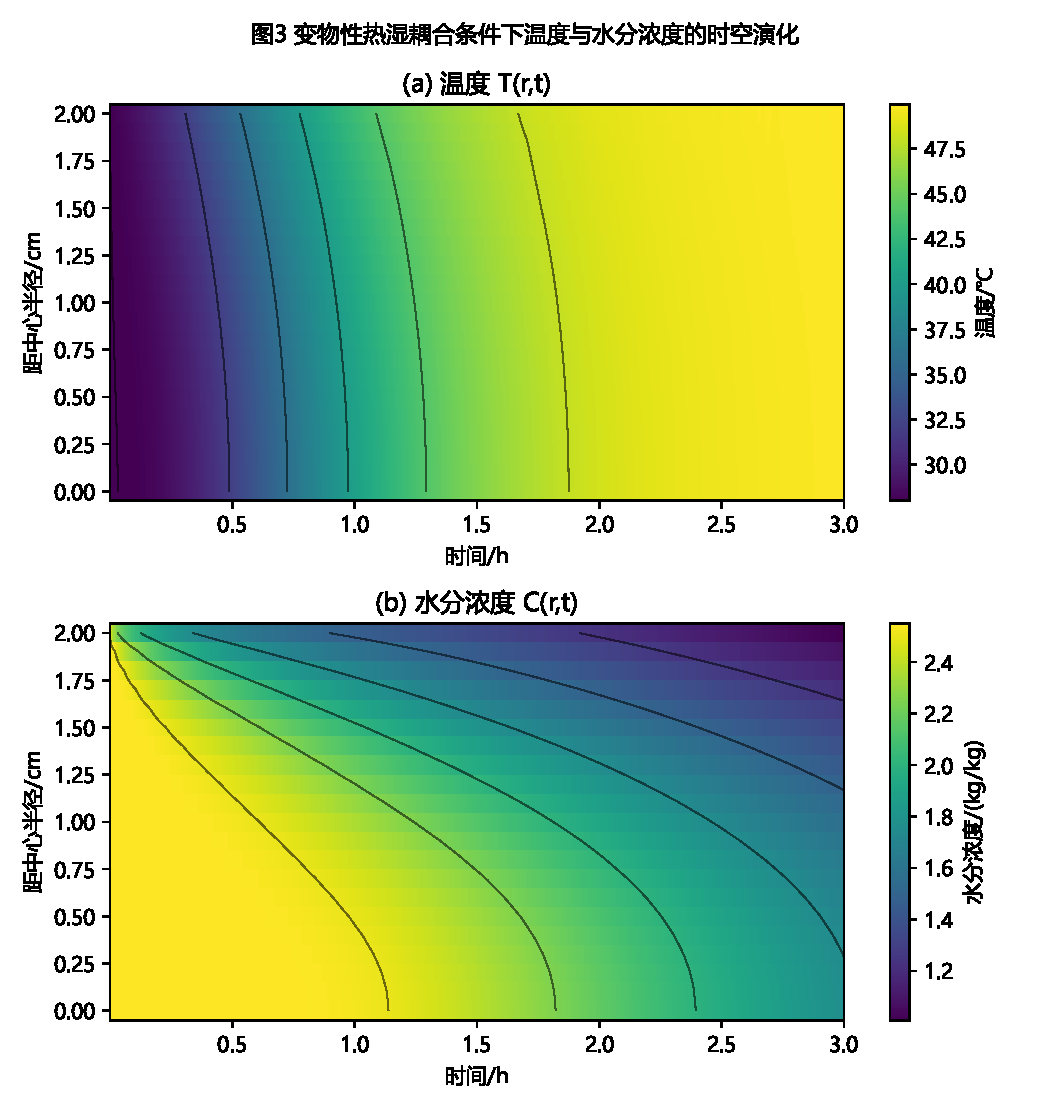
\includegraphics[width=0.88\textwidth]{figures/fig2_problem2_heatmap.pdf}
  \caption{变物性热湿耦合条件下温度与水分浓度的时空演化。(a) 温度 $T(r,t)$；(b) 水分浓度 $C(r,t)$；黑色细线为等值线。温度场约 $2\rm\,h$ 内接近烘房温度、径向梯度消失；水分场在整个 $3\rm\,h$ 内保持明显径向梯度，说明恒温干燥阶段受内部水分扩散控制。}
  \label{fig:q2-heatmap}
\end{figure}

\subsection{本问小结与后续衔接}
问题二完成了由常物性预热模型向变物性热湿耦合模型的过渡。计算结果显示，三小时内温度趋于均匀的速度明显快于水分扩散，后续达标时间将主要受中心区域含水率控制。因此，问题三不需要重新建立控制方程，只需在本问耦合模型基础上继续积分，并加入全截面达标事件。

\section{问题三模型的建立与求解}
\subsection{本问任务与前文承接}
问题三沿用问题二的固定半径耦合模型，目标由给定时刻输出转为达标时间定位。题目要求药材“各处”水分浓度均低于 $0.15\rm\,kg/kg$，因此本文不使用表面值或平均值作停机标准，而采用全截面最大水分浓度判据。

\subsection{模型建立}
令固定半径区域为
\begin{equation}
  \Omega_R=\{r\mid 0\le r\le R,\ R=0.02\rm\,m\},
\end{equation}
并定义连续全域最大含水率
\begin{equation}
  C_{\max}(t)=\max_{r\in\Omega_R}C(r,t).
\end{equation}
达标时间写为
\begin{equation}
  t^*=\inf\{t\ge0: C_{\max}(t)<C_{\rm cr}\},\qquad C_{\rm cr}=0.15\rm\,kg/kg.
\end{equation}
数值离散后，径向节点集为 $\mathcal R_h=\{r_i\}_{i=0}^{N-1}$，相应离散判据为
\begin{equation}
  C_{\max,h}(t)=\max_{r_i\in\mathcal R_h}C_i(t),\qquad
  g_h(t)=C_{\max,h}(t)-C_{\rm cr}.
\end{equation}
当 $g_h(t)$ 由正变负时，药材全截面达到题设水分要求。由于径向扩散路径最长的位置在中心，计算中通常有
\begin{equation}
  C_{\max,h}(t)=C(0,t),
\end{equation}
该关系也可作为结果合理性的检查。热量方程、水分方程、初始条件和第三类边界均沿用问题二；外部边界在 $t>4\rm\,h$ 时取附件1末值恒定外推，即仍采用式(2)。

\subsection{模型求解}
本问仍采用径向守恒 FVM。生产网格取
\begin{equation}
  \Delta r=0.00078125\rm\,cm,
  \qquad N=2561,
\end{equation}
联合状态为
\begin{equation}
  u(t)=\bigl[T_0(t),\ldots,T_{N-1}(t),C_0(t),\ldots,C_{N-1}(t)\bigr]^{\mathsf T}.
\end{equation}
时间推进采用自适应BDF，得到连续临界时间和离散临界时间，二者分别对应“连续事件定位”和“结果文件首个达标行”，后文分开报告。

实际求解时，固定半径网格取 $\Delta r=0.00078125\rm\,cm$、共 2561 个节点，联合状态初始化为 $u(0)=[T_0;C_0]$。BDF 积分器在 $g_h(t)$ 由正变负处进行步内事件定位，得到连续临界时间 $t^*$；随后按 $60\rm\,s$ 输出网格保存水分场，并抽取到题目指定半径位置。

为避免停机时间只依赖单一积分器，本文另用 backward-Euler + Picard 格式进行交叉验证。

\subsection{结果分析}
在附件1末值外推边界下，连续事件定位给出
\begin{equation}
  t^*=205821.7420\rm\,s=57.1727\rm\,h.
\end{equation}
终止时刻最大水分浓度出现在中心点，且
\begin{equation}
  C_{\max,h}(t^*)=C(0,t^*)=0.1499888\rm\,kg/kg<C_{\rm cr}.
\end{equation}
按 $60\rm\,s$ 输出网格向后取首个达标行，得到离散达标时刻
\begin{equation}
  t_{60}=205860\rm\,s=57.1833\rm\,h.
\end{equation}
因此，正文报告连续临界时间 $t^*$，结果文件末行采用 $t_{60}$。表\ref{tab:q3-moist} 中终止行中心值显示为 $0.1500$，来源于四舍五入；全精度值满足全域达标条件。

\begin{table}[H]
  \centering
  \caption{药材烘干过程的水分浓度 $/\rm kg\cdot kg^{-1}$}
  \label{tab:q3-moist}
  \begin{tabular}{rrrrrr}
    \toprule
    时间/h & 0 cm & 0.5 cm & 1 cm & 1.5 cm & 2 cm\\ \midrule
    6 & 1.0156 & 0.9868 & 0.9006 & 0.7546 & 0.5335\\
    12 & 0.4548 & 0.4418 & 0.4019 & 0.3289 & 0.1639\\
    18 & 0.2979 & 0.2906 & 0.2679 & 0.2247 & 0.0842\\
    24 & 0.2371 & 0.2321 & 0.2161 & 0.1851 & 0.0663\\
    30 & 0.2053 & 0.2013 & 0.1887 & 0.1637 & 0.0597\\
    36 & 0.1854 & 0.1821 & 0.1714 & 0.1501 & 0.0565\\
    42 & 0.1717 & 0.1687 & 0.1593 & 0.1404 & 0.0547\\
    48 & 0.1615 & 0.1588 & 0.1504 & 0.1332 & 0.0536\\
    54 & 0.1535 & 0.1511 & 0.1433 & 0.1275 & 0.0528\\
    57.1727 & 0.1500 & 0.1477 & 0.1402 & 0.1249 & 0.0525\\
    \bottomrule
  \end{tabular}
\end{table}

表\ref{tab:q3-moist} 中，表面点在 $18\rm\,h$ 已降至 $0.0842\rm\,kg/kg$，中心点仍为 $0.2979\rm\,kg/kg$；到 $54\rm\,h$，表面点为 $0.0528\rm\,kg/kg$，中心点仍为 $0.1535\rm\,kg/kg$。这说明固定半径模型的停机时间主要由中心控制，可概括为
\begin{equation}
  C(R,t)<C_{\rm cr}\ \not\Rightarrow\ C_{\max}(t)<C_{\rm cr}.
\end{equation}
图\ref{fig:q3-event} 中，$C=C_{\rm cr}$ 等值线由表面向中心收缩，进一步说明干燥前沿自外向内推进；连续临界时间 $t^*$ 对应积分器的连续事件定位，离散输出时刻 $t_{60}$ 对应结果文件中的首个达标行。

\begin{figure}[H]
  \centering
  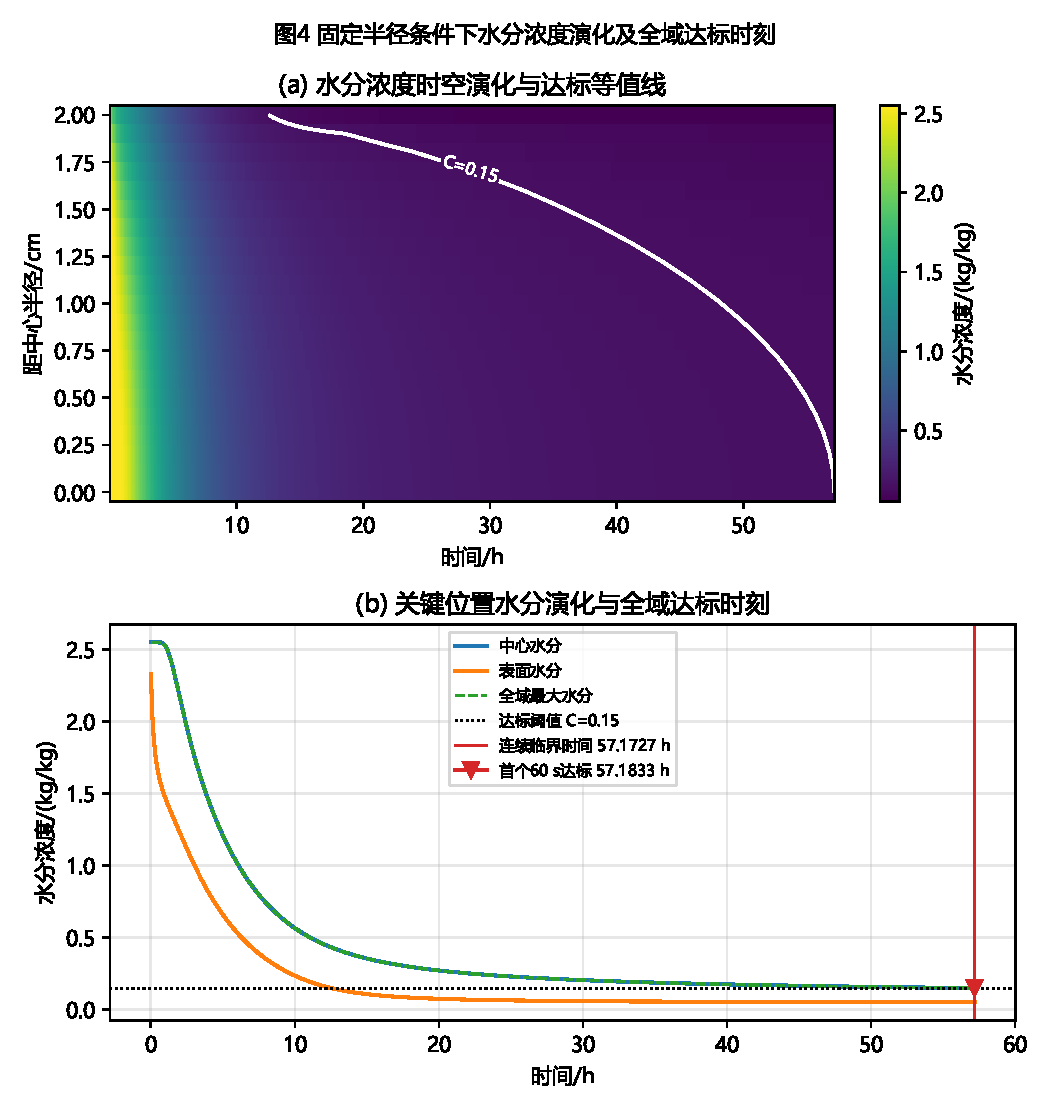
\includegraphics[width=0.88\textwidth]{figures/fig3_problem3_event.pdf}
  \caption{固定半径条件下水分浓度演化及全域达标时刻。(a) 水分浓度时空热力图，白色曲线为 $C=0.15\rm\,kg/kg$ 达标等值线；(b) 中心、表面与全域最大水分随时间演化，水平点线为达标阈值，竖线与三角标记分别给出连续临界时间与首个 $60\rm\,s$ 达标时刻。}
  \label{fig:q3-event}
\end{figure}

为区分边界假设与数值误差，记边界情景集合为
\begin{equation}
  \mathcal S=\{(\Delta T_\infty,\eta_C):\Delta T_\infty\in\{-2,0,2\},\ \eta_C\in\{0.9,1.0,1.1\}\}.
\end{equation}
在该集合上重算得
\begin{equation}
  t^*(\mathcal S)\in[53.6154,61.0702]\rm\,h.
\end{equation}
若只扰动 $h_m$ 的 $\pm10\%$，则
\begin{equation}
  t^*\in[56.5955,57.9086]\rm\,h.
\end{equation}
而数值误差量级为
\begin{equation}
  |t^*_{\rm BDF}-t^*_{\rm BE}|=7.95\rm\,s,
  \quad |t^*_h-t^*_{\rm Rich}|\approx10\rm\,s,
  \quad |t^*_{h}-t^*_{2h}|=39.34\rm\,s.
\end{equation}
可见，边界外推带来的小时级变化显著大于数值离散误差。因此，$57.1727\rm\,h$ 是末值外推边界下的点估计，上述边界情景区间用于描述外部边界不确定性。

\subsection{本问小结与后续衔接}
问题三在固定半径、附录3物性和末值外推边界下得到
\begin{equation}
  t^*=57.1727\rm\,h,\qquad t^*(\mathcal S)\in[53.6154,61.0702]\rm\,h.
\end{equation}
该结果构成问题四移动边界模型的固定半径基准。问题四将在同一全截面判据下引入 $R(t)$ 和附录4物性，比较收缩对达标时间的影响。
\section{问题四模型的建立与求解}
\subsection{本问任务与前文承接}
问题四在问题三达标停机框架上进一步引入半径收缩。与问题三相比，本问同时发生两类变化：物性关系由附录3改为附录4，几何边界由固定半径 $R=2.0\rm\,cm$ 改为附件2给定的时变半径 $R(t)$。半径收缩会改变扩散距离和表面位置，若仍在物理半径上直接离散，需要不断移动网格。为保持计算网格稳定，本文将移动物理域映射到固定计算域，并在相同全截面含水率阈值下求解临界时间。

\subsection{建模思路}
移动边界处理的核心，是把随时间变化的物理区间 $r\in[0,R(t)]$ 化为固定区间。本文采用 Landau 前置固定变换，引入物质坐标
\begin{equation}
  \xi=\frac{r}{R(t)}\in[0,1],
\end{equation}
从而把收缩域映射到 $\xi\in[0,1]$。在均匀径向收缩假设下，$\xi$ 表示同一物质层的位置标签；干基含水率 $C$ 以单位干物质质量为基准，也适合在物质坐标下跟踪。对守恒式作物质导数处理后，收缩效应主要体现在两个位置：内部扩散项出现尺度因子 $1/R^2(t)$，表面通量项出现尺度因子 $R(t)$。采用这一坐标后，无需额外引入由网格收缩产生的对流项。

需要说明的是，附件2的 $R(t)$ 在本文中作为题目给定的经验输入，并非由含水率场反推的未知量。附录4密度律与附件2半径轨迹是否严格满足干物质质量守恒，不作为本问求解的约束条件；该一致性问题在后文模型检验与评价中单独讨论。

与固定半径模型相比，问题四临界时间由 $57.1727\rm\,h$ 缩短至 $50.8245\rm\,h$。这一差异并非单纯来自物性参数改变，而与半径收缩引起的特征扩散尺度变化密切相关。为直观说明半径收缩对内部水分迁移及最终达标时间的作用路径，其主要机制概括如图\ref{fig:q4-shrinkage-mechanism}所示。

\begin{figure}[H]
  \centering
  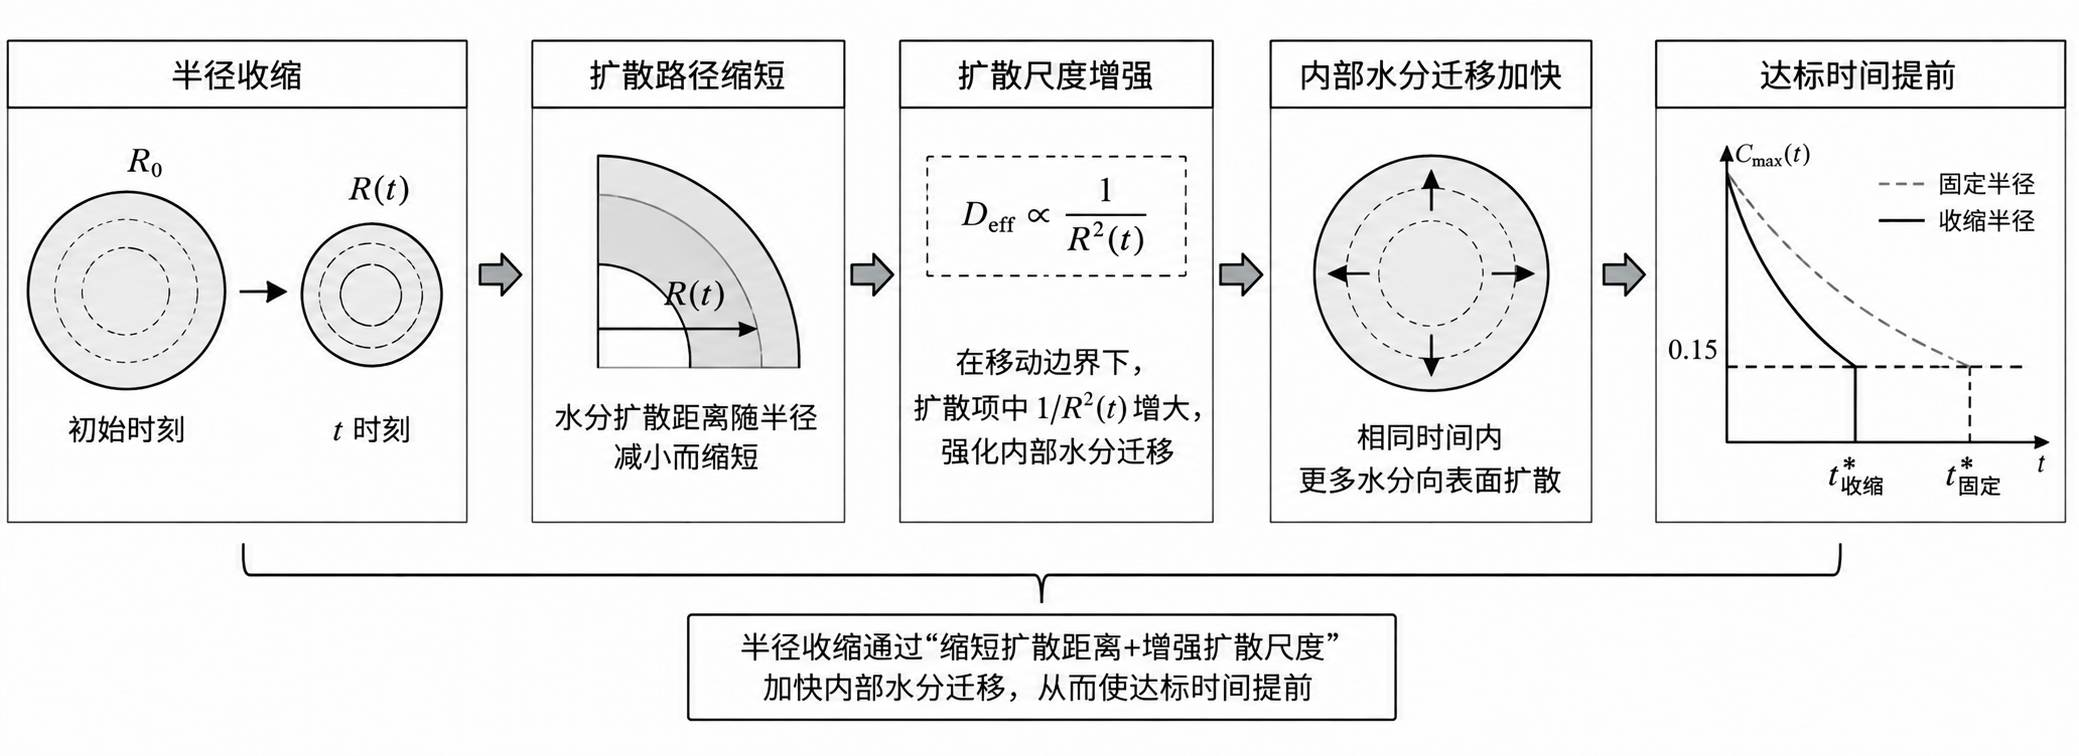
\includegraphics[width=\textwidth]{figures/shrinkage_mechanism.jpg}
  \caption{半径收缩促进内部水分迁移并缩短达标时间的作用机制}
  \label{fig:q4-shrinkage-mechanism}
\end{figure}

如图\ref{fig:q4-shrinkage-mechanism}所示，随着药材半径由 $R_0$ 缩小至 $R(t)$，中心水分迁移至表面的有效扩散距离随之缩短；在物质坐标表示下，扩散项的特征尺度又随
\[
  \frac{1}{R^2(t)}
\]
增大，从而强化单位物质坐标尺度上的水分迁移。两种作用共同促进内部高含水区域更快向表面释放水分，使全域最大含水率更早降至规定阈值。因此，在题设给定半径轨迹及附录4物性关系下，收缩模型的连续达标时间为 $50.8245\rm\,h$，较问题三固定半径模型的 $57.1727\rm\,h$ 提前约 $6.35\rm\,h$。

\subsection{模型建立}
附录4给出的状态相关物性为
\begin{equation}
  \rho(C)=760+90C,\qquad
  c_p(C)=1850+\frac{2150C}{C+1},\qquad
  k(C)=0.12+\frac{0.20C}{C+1},
\end{equation}
\begin{equation}
  D(C,T)=4.2\times10^{-4}\exp\left(-\frac{0.30}{C}\right)
  \exp\left(-\frac{3850}{T_K}\right),\qquad T_K=T+273.15.
\end{equation}
在物质坐标 $\xi$ 下，温度场与水分场可统一写为压缩扩散方程：
\begin{equation}
  \left.\frac{\partial u}{\partial t}\right|_{\xi}
  =\frac{1}{\mathrm{cap}\cdot\xi R^2}
  \frac{\partial}{\partial\xi}\left(\xi\,\mathrm{cond}\,\frac{\partial u}{\partial\xi}\right),
\end{equation}
其中 $u=T$ 时 $\mathrm{cap}=\rho(C)c_p(C)$、$\mathrm{cond}=k(C)$；$u=C$ 时 $\mathrm{cap}=1$、$\mathrm{cond}=D(C,T)$；$R(t)$ 由附件2线性插值得到。初始条件为 $T(\xi,0)=28$、$C(\xi,0)=2.55$。中心 $\xi=0$ 为对称零通量边界；表面 $\xi=1$（即 $r=R(t)$）为第三类边界
\begin{equation}
  -\mathrm{cond}\left.\frac{\partial u}{\partial\xi}\right|_{\xi=1}
  =\mathrm{transfer}\cdot R(t)\cdot\left(u_s-u_{\rm ext}\right),
\end{equation}
其中温度场 $\mathrm{transfer}=h$、$u_{\rm ext}=T_\infty(t)$，水分场 $\mathrm{transfer}=h_m$、$u_{\rm ext}=C_\infty(t)$。$4\rm\,h$ 后的烘房边界与问题三一致，取附件1末值恒定外推。

收缩和物性切换对达标时间的影响方向并不完全相同。半径收缩通过 $1/R^2(t)$ 增大有效扩散尺度，并缩短中心到表面的距离；而附录4中的扩散系数基值 $4.2\times10^{-4}$ 小于附录3中的 $2.4\times10^{-3}$，会降低相同状态下的水分迁移速率。二者共同决定本问相对于问题三是提前还是延后达标。停机判据仍取全剖面最大水分浓度，首次满足 $C_{\max}(t)<0.15\rm\,kg/kg$ 时停止积分。

\subsection{模型求解}
在完成移动边界坐标变换及控制方程构建后，问题四的数值求解还需同步处理时变环境边界、半径轨迹、状态相关物性以及全域达标事件。为明确各计算模块之间的数据传递关系，本文将移动边界模型的完整数值求解过程整理如图\ref{fig:q4-solver-flow}所示。

\begin{figure}[H]
  \centering
  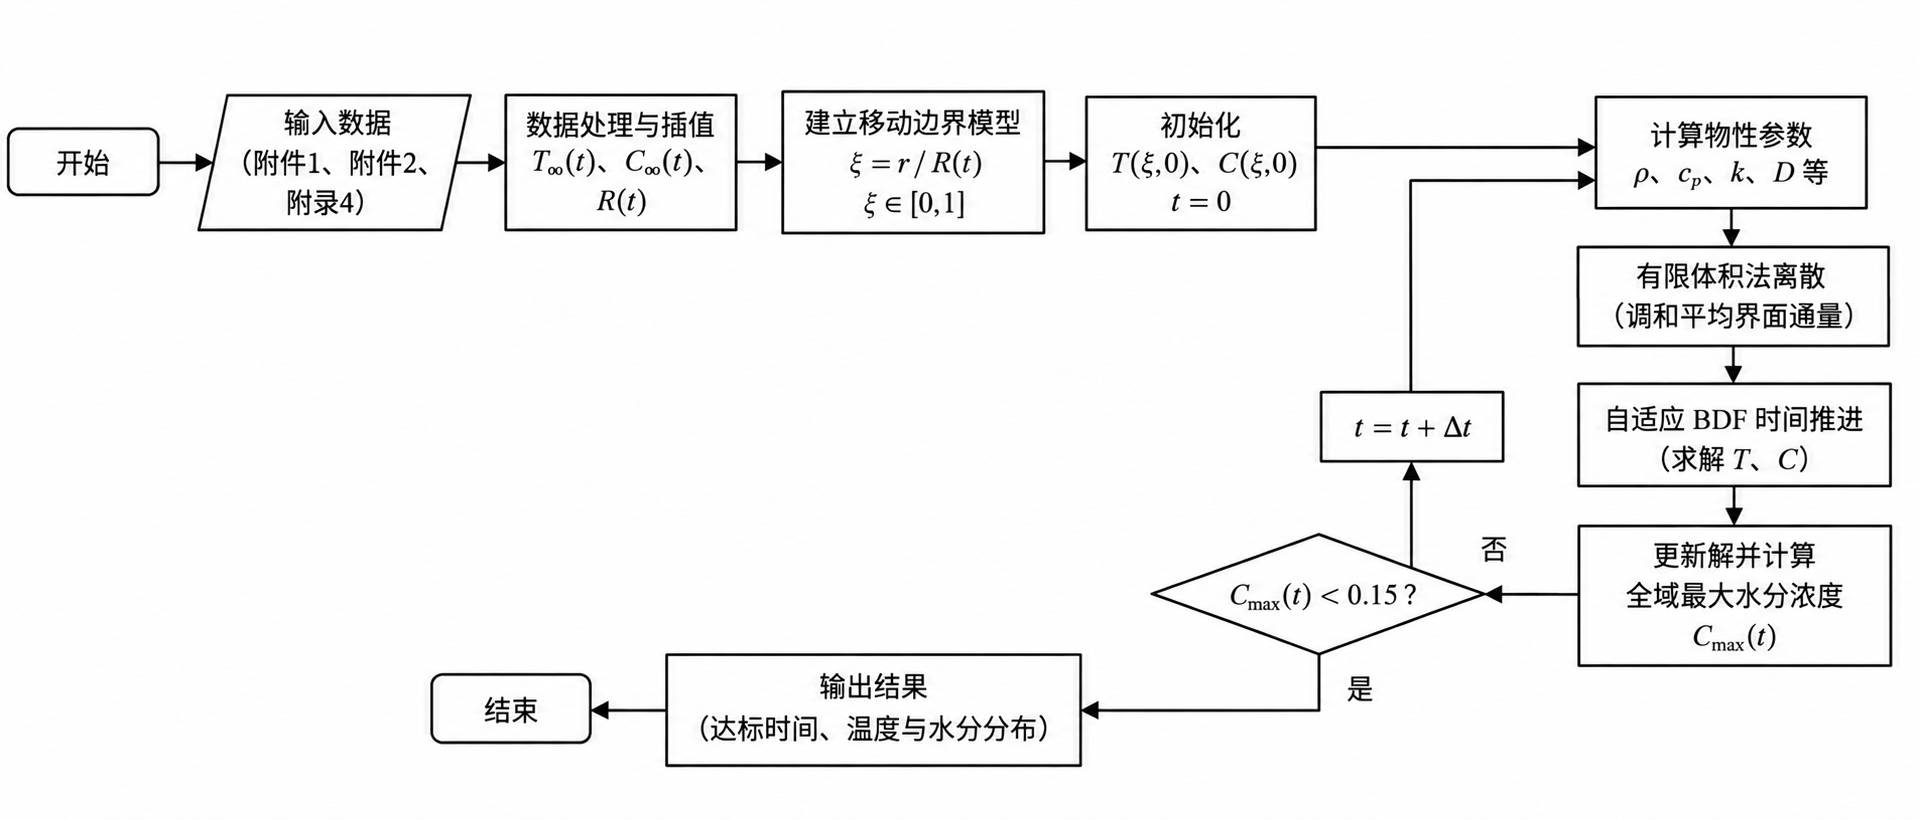
\includegraphics[width=\textwidth]{figures/q4_solver_flow.jpg}
  \caption{基于物质坐标变换与自适应 BDF 的问题四数值求解流程}
  \label{fig:q4-solver-flow}
\end{figure}

如图\ref{fig:q4-solver-flow}所示，首先对附件中的烘房温度、环境水分浓度及半径数据进行处理与插值，并利用
\[
  \xi=\frac{r}{R(t)}
\]
将时变物理区域映射至固定计算域；随后根据当前温度、水分状态更新密度、比热容、热导率及扩散系数，并采用守恒型有限体积法完成空间离散。时间方向由自适应 BDF 隐式推进，每一时刻更新温度场与水分场后计算全域最大水分浓度 $C_{\max}(t)$。当
\[
  C_{\max}(t)<0.15
\]
时触发终止事件并输出达标时间，否则继续推进至下一时刻。该流程实现了移动边界、变物性热湿耦合与连续终点判定的统一求解。

问题四在固定 $\xi$ 网格上采用严格径向守恒有限体积法。计算条件包括初值 $T_0,C_0$、附录4物性、附件1环境边界及末值外推规则，以及附件2半径序列 $R(t)$；计算结果包括连续临界时间 $t^*$ 和含移动表面列的水分浓度过程表。

生产计算采用固定的 $\xi$ 网格：
\begin{equation}
  N=3201,\qquad \Delta\xi=\frac{1}{N-1}.
\end{equation}
控制体几何量和界面面积分别为
\begin{equation}
  \hat V_i=\frac12\left(\xi_{i+1/2}^2-\xi_{i-1/2}^2\right),\qquad
  \hat A_{i+1/2}=\xi_{i+1/2}.
\end{equation}
上述几何量相当于在单位 $\xi$ 圆盘上组装径向守恒通量。界面热导率 $k$ 和扩散系数 $D$ 均采用调和平均，以降低强梯度区域的界面通量高估风险。

时间推进仍采用 \texttt{scipy.integrate.solve\_ivp} 的联合状态自适应 BDF 隐式积分器，计算参数为
\begin{equation}
  \mathrm{rtol}=10^{-8},\qquad
  \mathrm{atol}_T=10^{-8},\qquad
  \mathrm{atol}_C=10^{-10},\qquad
  \Delta t_{\max}=30\rm\,s.
\end{equation}

每个时间步由附件2线性插值得到当前 $R(t)$，并据此更新有效扩散系数 $\mathrm{cond}/R^2$ 和表面对流尺度 $\mathrm{transfer}\cdot R$；同时由当前联合状态计算 $\rho(C),c_p(C),k(C),D(C,T+273.15)$，再用调和平均组装界面通量。中心 $\xi=0$ 用对称零通量条件消除奇点，表面 $\xi=1$ 施加第三类边界；块三对角稀疏 Jacobian 由解析式提供。

终止事件及其搜索方向设为
\begin{equation}
  g(t)=\max_\xi C(\xi,t)-0.15,\qquad
  \texttt{terminal=True},\qquad \texttt{direction}=-1.
\end{equation}
到达 $60\rm\,s$ 输出间隔时，程序按固定距离 $d=\xi R(t)$ 记录水分浓度，若指定距离已超过当前半径，则该位置不再属于药材内部。

为验证物质坐标实现，程序还进行了 $D=0$ 时物质剖面守恒自检，并以 backward-Euler + Picard 固定步隐式格式作为独立对照。

BDF 积分触发终止事件后得到连续临界时间。内部通量平衡的最大归一化残差为 $2.087\times10^{-16}$，处于机器精度量级。

最小原始水分为 $0.0525\rm\,kg/kg$，计算过程中未触发非负裁剪；全域最大含水率始终位于中心 $\xi=0$，与圆柱径向扩散的滞后规律一致。

backward-Euler + Picard 对照在 $\Delta t=20/10/5/2.5\rm\,s$ 四档时间步下分别给出 $t^*=50.8377/50.8312/50.8279/50.8262\rm\,h$，随时间步减小向 BDF 结果收敛；最细 BE 与 BDF 相差 $6.15\rm\,s$，相对差为 $3.36\times10^{-5}$。

\subsection{结果分析}
计算得到
\begin{equation}
  t^*=182968.2250\rm\,s=50.8245\rm\,h.
\end{equation}
半径从首次采样时刻的 $1.9958\rm\,cm$ 收缩到临界时刻的约 $1.2000\rm\,cm$。临界时刻中心全精度含水率已低于 $0.15\rm\,kg/kg$，表中显示 $0.1500$ 来自四舍五入。第一个在 $60\rm\,s$ 输出网格上严格达标的时刻为 $183000\rm\,s=50.8333\rm\,h$，即 \texttt{result4.xlsx} 的末行。表\ref{tab:q4-moist} 按题目要求给出每 $6\rm\,h$ 及临界时刻、固定距离 $0$、$0.5$、$1\rm\,cm$ 与移动表面处的水分浓度。由于半径在后期已降至 $1.5\rm\,cm$ 以下，更远的固定距离已不在药材内部，该处状态应由烘房环境而非药材内部方程描述，故表中不再列出，不属于数据缺失。

\begin{table}[H]
  \centering
  \caption{药材烘干过程的水分浓度（含半径收缩·移动表面）$/\rm kg\cdot kg^{-1}$}
  \label{tab:q4-moist}
  \begin{tabular}{rrrrr}
    \toprule
    时间/h & 0 cm & 0.5 cm & 1 cm & 药材表面\\ \midrule
    6 & 1.7172 & 1.5357 & 1.0217 & 0.4217\\
    12 & 0.7343 & 0.6518 & 0.4069 & 0.1667\\
    18 & 0.4066 & 0.3668 & 0.2388 & 0.0889\\
    24 & 0.2837 & 0.2599 & 0.1783 & 0.0671\\
    30 & 0.2253 & 0.2085 & 0.1488 & 0.0593\\
    36 & 0.1921 & 0.1790 & 0.1312 & 0.0558\\
    42 & 0.1706 & 0.1598 & 0.1196 & 0.0539\\
    48 & 0.1556 & 0.1463 & 0.1113 & 0.0529\\
    50.8245 & 0.1500 & 0.1413 & 0.1081 & 0.0525\\
    \bottomrule
  \end{tabular}
\end{table}

\begin{figure}[H]
  \centering
  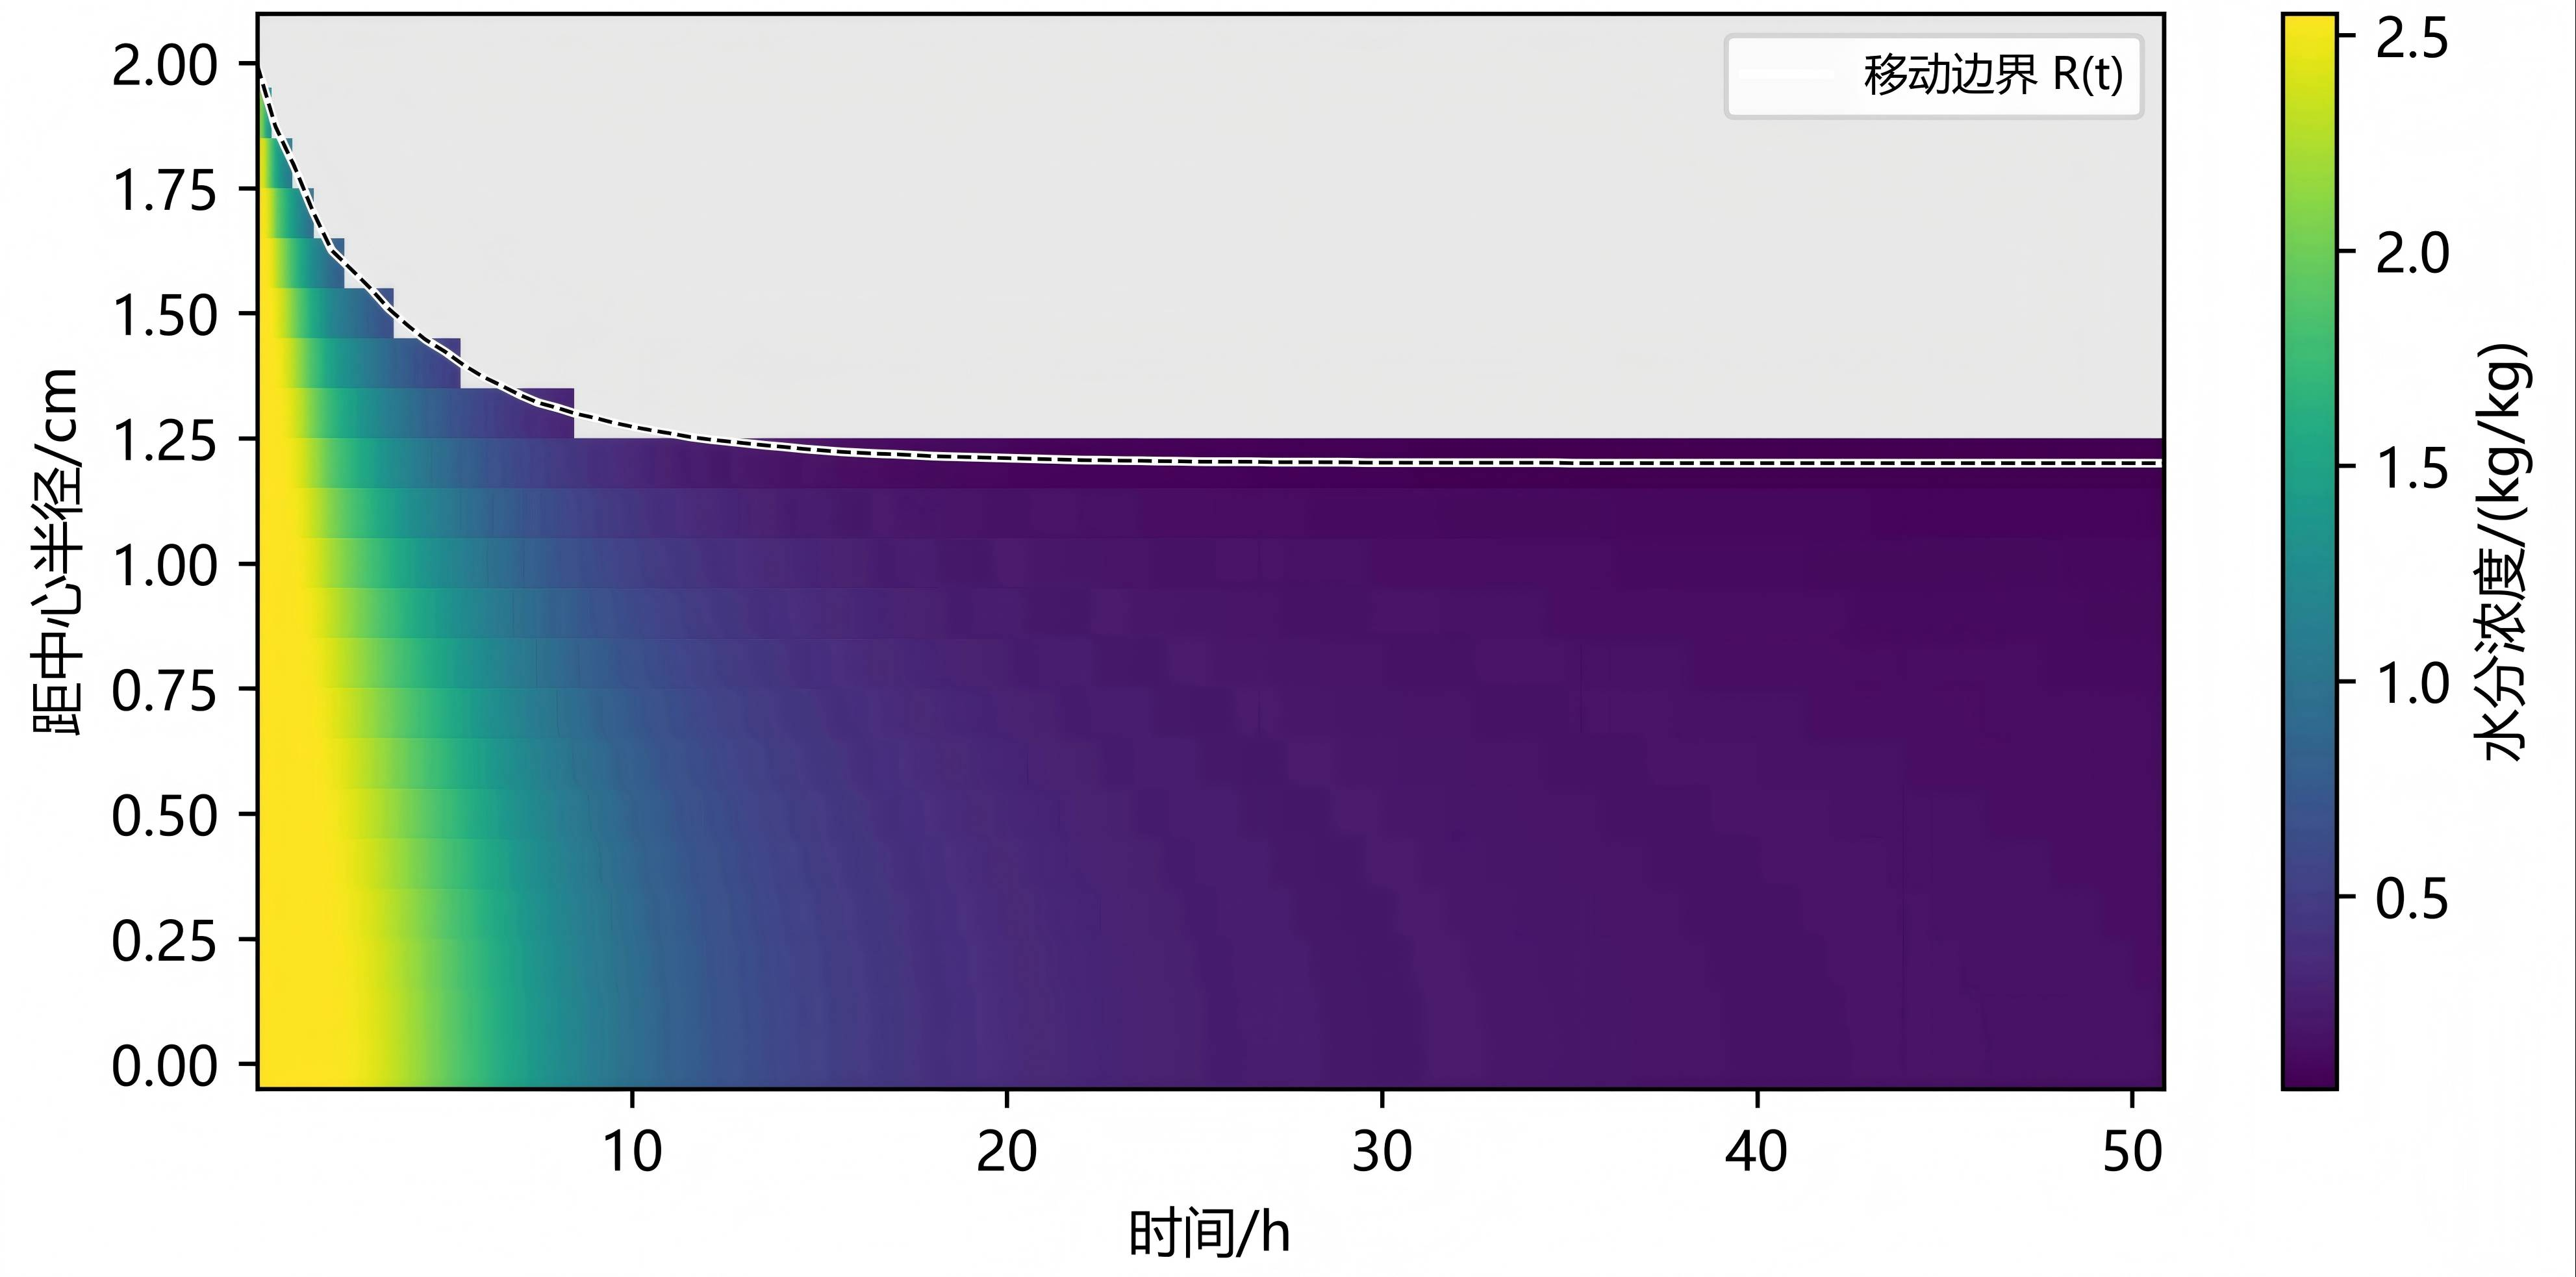
\includegraphics[width=0.88\textwidth]{figures/fig4_problem4_moving_boundary.jpg}
  \caption{半径收缩条件下物理坐标中的水分浓度演化。白色曲线为移动边界 $R(t)$，灰色为已收缩退出的药材区域。}
  \label{fig:q4-moving}
\end{figure}

图\ref{fig:q4-moving} 中，移动边界 $R(t)$ 从 $2.0\rm\,cm$ 收缩至临界时刻的约 $1.2\rm\,cm$，灰色区域为已收缩退出的药材区域。剩余区域内水分浓度仍呈中心高、表面低的分布形态；表面含水率后期接近 $0.0525\rm\,kg/kg$，与环境末值 $0.04986\rm\,kg/kg$ 相近，而中心含水率下降较慢并继续控制终止时刻。

边界情景分析给出了默认答案的外部适用范围。将 $4\rm\,h$ 后温度扰动 $\pm2^\circ\mathrm C$、水分扰动 $\pm10\%$ 组成 $3\times3$ 情景时，$t^*$ 落在 $47.6834$--$54.2753\rm\,h$；传质系数 $h_m$ 扰动 $\pm10\%$ 时，$t^*$ 落在 $50.6035$--$51.1159\rm\,h$；用附件最后 $30$ 分钟或 $1\rm\,h$ 均值延拓代替末值外推时，$t^*$ 为 $51.0757$--$51.0972\rm\,h$。与这些小时量级的边界差异相比，数值离散误差较小：网格 $201\to3201$ 的末级差为 $3.30\rm\,s$，BDF 容差三档差小于 $2\times10^{-4}\rm\,s$，BDF 与 BE-Picard 对照差为 $6.15\rm\,s$。因此，$50.8245\rm\,h$ 可作为题设默认边界下的点估计，边界情景区间用于说明后期烘房条件外推带来的不确定性。

\subsection{本问小结与后续衔接}
问题四通过物质坐标前置固定，将半径收缩问题转化为固定域上的压缩扩散问题，并在同一全截面达标判据下得到连续临界时间 $t^*=50.8245\rm\,h$。该时间短于问题三固定半径结果 $57.1727\rm\,h$，说明在题设半径轨迹和附录4物性下，扩散路径缩短带来的加速作用占主导。后续模型检验与评价将进一步讨论数值收敛、坐标解释差异以及附件2半径轨迹与附录4密度律之间的闭合关系。

\section{模型的检验与分析}
\subsection{数值收敛检验}
为确认计算结果不受离散设置支配，本文从空间网格、时间精度和独立求解器三个方面进行检验。

为排除空间离散尺度和时间推进策略对临界时间结果的主导影响，本文进一步从空间网格加密和独立时间积分格式两个层面开展收敛性检验。问题三考察固定半径条件下临界时间随径向网格尺度的变化，问题四考察移动边界模型随物质坐标节点数增加的收敛趋势，并采用后向欧拉（BE）与 BDF 两种隐式格式进行交叉验证，结果如图\ref{fig:convergence-crossvalidation}所示。

\begin{figure}[H]
  \centering
  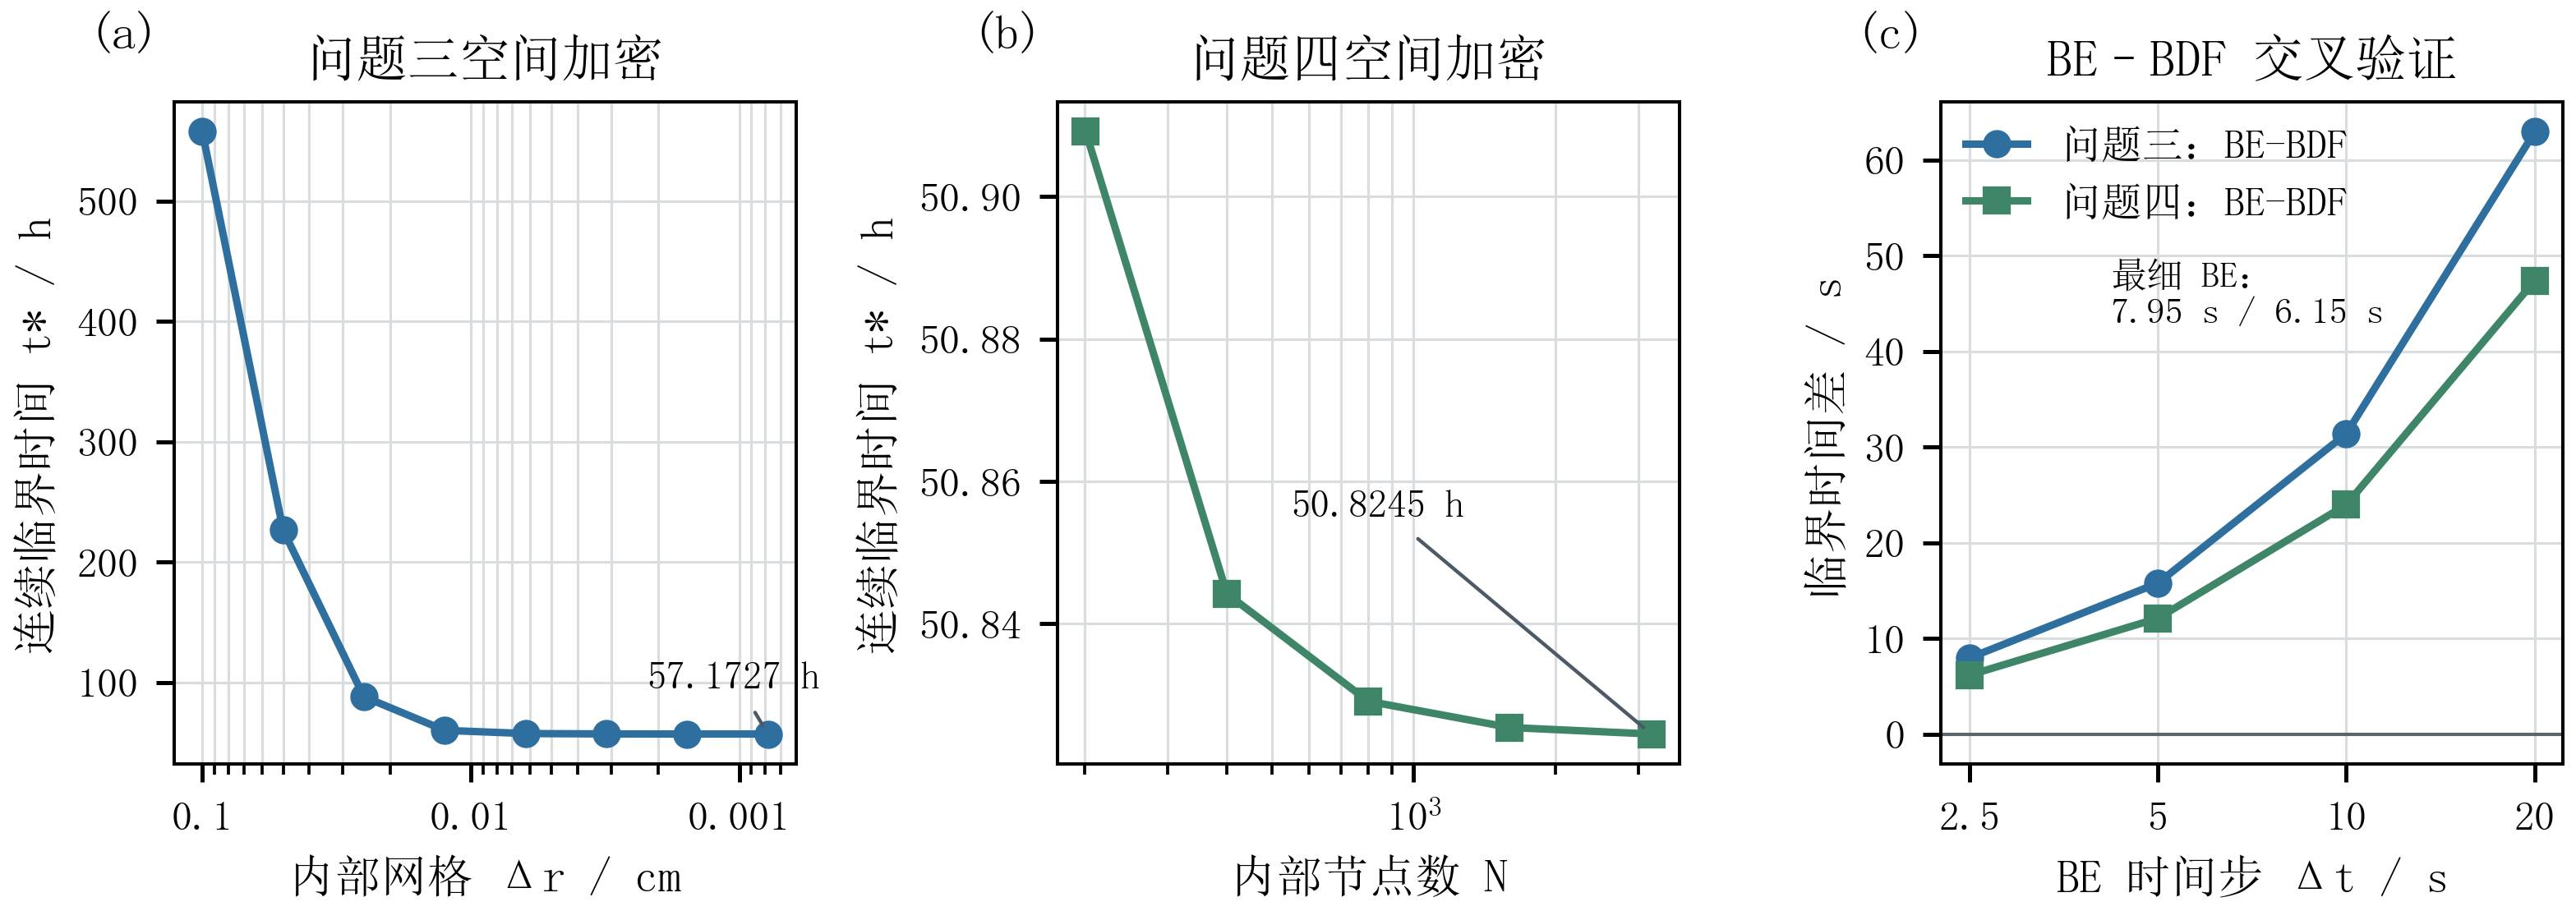
\includegraphics[width=\textwidth]{figures/convergence_validation.jpg}
  \caption{空间离散与时间积分的数值收敛及交叉验证结果}
  \label{fig:convergence-crossvalidation}
\end{figure}

图\ref{fig:convergence-crossvalidation}(a)表明，随着问题三内部径向网格持续加密，连续临界时间逐渐收敛至 $57.1727\rm\,h$；图\ref{fig:convergence-crossvalidation}(b)显示，问题四在增加物质坐标节点数后，临界时间稳定于 $50.8245\rm\,h$ 附近。与此同时，图\ref{fig:convergence-crossvalidation}(c)中 BE 与 BDF 两种时间推进方法在步长减小时均表现出一致的收敛趋势。上述结果说明，本文最终临界时间并非由特定网格尺度或单一时间积分器偶然产生，数值离散误差已被控制在远低于边界条件不确定性的水平。

问题一将内部网格继续加密后，温度和水分的最大变化均不超过 $1.90\times10^{-4}$；界面扩散系数改用调和平均所引起的变化也低于报告精度。因此，正文表格中的四位小数保持稳定。

问题二采用两级网格比较，温度和水分的最大差均小于 $5\times10^{-5}$。进一步收紧 BDF 容差并缩小最大步长后，表中数值在四位小数下没有变化。

问题三对网格更敏感。末两级网格的事件时间相差 $39.34\rm\,s$，生产网格与 Richardson 外推值相差 $10.01\rm\,s$；严格 BDF 与后向欧拉--Picard 的结果相差 $7.95\rm\,s$。三种检验给出的误差均处于可接受范围。

调和平均需要与足够细的网格配合。若直接在 $0.1\rm\,cm$ 粗网格上计算，会把近表面的低扩散区域集中为过大的界面阻力，得到 $557.4174\rm\,h$ 的异常结果；持续加密后，终止时间稳定收敛到 $57.1727\rm\,h$。因此，粗网格结果不具有物理解释意义。

问题四的末两级网格结果相差 $3.30\rm\,s$，最细后向欧拉结果与 BDF 相差 $6.15\rm\,s$。计算过程中水分剖面保持单调，最大含水率始终位于中心，说明事件判据与径向扩散规律一致。

\subsection{问题四两种坐标模型的结果比较}
问题四以物质坐标 FVM-BDF 为主模型。由于题目未给出内部形变速度场，本文另计算 Euler 空间坐标模型，用于考察坐标解释对结果的影响。表\ref{tab:q4-coord}仅作敏感性比较，不表示两个结果均为答案。

\begin{table}[htbp]
  \centering
  \caption{问题四两种坐标模型的结果比较}
  \label{tab:q4-coord}
  \small
  \begin{tabular}{lcp{6.5cm}}
    \toprule
    模型 & $t^*$/h & 说明\\
    \midrule
    物质坐标 FVM-BDF 模型 & \textbf{50.8245} & 问题四最终结果\\
    Euler 空间坐标模型 & 52.3842 & 坐标处理敏感性对照，不纳入主答案\\
    \bottomrule
  \end{tabular}
\end{table}

物质坐标模型以 $\xi=r/R(t)$ 标记同一物质层，符合均匀径向收缩假设，得到 $t^*=50.8245\rm\,h$。Euler 空间坐标模型保留收缩对流项，结果比主模型晚 $1.5597\rm\,h$，反映了内部形变场未知带来的模型形式敏感性。

作为数值实现互证，固定步后向欧拉--Picard 方案与 FVM-BDF 主结果仅相差 $0.0301\rm\,h$，约为 $0.06\%$。由此可见，数值实现差异小于坐标解释和边界假设造成的影响。

\subsection{边界敏感性讨论}
问题三和问题四的计算时长均超过附件1覆盖的前 $4\rm\,h$，后期结果因而依赖边界末值外推。边界敏感性分析用于把这一外部假设的影响与数值误差区分开。

当后期温度扰动 $\pm2^\circ\mathrm C$、环境水分扰动 $\pm10\%$ 时，问题三的达标时间为 $53.6154$--$61.0702\rm\,h$，问题四为 $47.6834$--$54.2753\rm\,h$。其中温度变化的影响更明显，传质系数扰动和不同末值平均方式造成的变化相对较小。

上述情景变化达到小时量级，而网格和求解器误差主要处于秒级。因此，$57.1727\rm\,h$ 和 $50.8245\rm\,h$ 应理解为末值外推条件下的点估计；敏感性范围只说明边界假设的影响，不代表统计置信区间。

问题四表格只列至 $1\rm\,cm$ 固定距离并附移动表面，是因为更远的位置在后期已退出药材内部，并非数据缺失。

\subsection{物理合理性检验}
四问呈现出一致的物理规律：外部热风先影响表面，中心响应较慢。温度场较早趋于均匀，而水分梯度持续时间更长，最终由中心含水率控制停机。

问题四中，半径收缩缩短了水分传递路径，使达标时间早于固定半径情形。这些现象符合圆柱径向扩散和移动边界的基本规律。

\section{模型评价}
\subsection{模型优点}
\begin{enumerate}[label=\arabic*、,leftmargin=2.5em,itemsep=0.4em]
  \item 四问采用统一的径向有限体积框架，模型层次清楚，前后衔接自然。
  \item 联合求解温度与水分状态，能够反映变物性条件下的热湿相互影响。
  \item 停机判据面向全截面，并通过网格加密和独立求解器检验结果稳定性。
\end{enumerate}

\subsection{模型不足}
\begin{enumerate}[label=\arabic*、,leftmargin=2.5em,itemsep=0.4em]
  \item 后期环境条件采用末值外推，难以反映实际烘房温湿度的持续波动。
  \item 受题给参数限制，模型未显式描述蒸发潜热，收缩与密度关系也未完全闭合。
\end{enumerate}

\subsection{模型的推广}
本模型可用于其他圆柱状物料的热风干燥预测；更换物性、尺寸、边界条件和达标阈值后，即可重新计算温湿分布与停机时间。

\section{AI 工具使用声明}
本参赛队在竞赛过程中使用了AI工具，主要用于思路梳理、代码辅助编写与调试、数值结果复核、格式检查，详细使用情况见支撑材料。

\section{参考文献}
\begin{enumerate}[label={[\arabic*]},leftmargin=3em,itemsep=0pt,topsep=0pt]
  \item 刘琦. 基于有限体积法非傅里叶导热及热粘弹性耦合问题的研究[D]. 哈尔滨工程大学, 2020.
  \item 单惠敏. 香菇热风烘干实验与数值模拟[D]. 湖南科技大学, 2021.
  \item 庞凌云, 袁志华, 詹丽娟, 等. 铁棍山药片热风干燥过程中传热传质规律[J]. 食品与机械, 2024, 40(8): 157--165.
  \item Morris D E. Factorial sampling plans for preliminary computational experiments. \textit{Technometrics}, 1991, 33(2): 161--174.
  \item Xiu D, Karniadakis G E. The Wiener-Askey polynomial chaos for stochastic differential equations. \textit{SIAM Journal on Scientific Computing}, 2002, 24(2): 619--644.
  \item Sobol I M. Global sensitivity indices for nonlinear mathematical models and their Monte Carlo estimates. \textit{Mathematics and Computers in Simulation}, 2001, 55(1--3): 271--280.
  \item Saltelli A, Annoni P, Azzini I, Campolongo F, Riva M, Tarantola S. Variance based sensitivity analysis of model output: Design and estimator for the total sensitivity index. \textit{Computer Physics Communications}, 2010, 181(2): 259--270.
\end{enumerate}

% ========== 附录A ==========
\newpage
\begin{center}
  \Large\bfseries 附录A：支撑材料清单
\end{center}
\vspace{1em}

\begin{table}[h]
\centering
\renewcommand{\arraystretch}{1.3}
\begin{tabular}{lp{10cm}}
\toprule
\textbf{文件名} & \textbf{说明} \\
\midrule
problem1.py & 问题一求解器：径向 FVM + BDF 时间推进，输出温度场与水分场 \\
problem2.py & 问题二求解器：变物性耦合模型，输出中心温度与干燥时间 \\
problem3.py & 问题三求解器：严格径向 FVM + BDF，含后向欧拉交叉验证 \\
problem4.py & 问题四求解器：动边界 FVM + BDF，多情景模拟 \\
sensitivity.py & 全局敏感性分析：Morris 筛选 + PCE-Sobol 指数 + Radau 交叉验证 \\
figures.py & 论文插图生成脚本（图1–图5） \\
limitations.py & 模型局限性分析：干物质闭合、潜热影响、半径上限证明 \\
mass\_closure.py & 质量闭合验证：干物质守恒与水分平衡核算 \\
bonus.py & 附加验证：Bessel 解析模态、时间推进阶数、参数敏感性 \\
交叉验证.py & BE-BDF 交叉验证绘图与误差分析 \\
result1.xlsx & 问题一数值结果（温度场、水分场随时间演化） \\
result2.xlsx & 问题二数值结果（中心温度、干燥时间表） \\
result3.xlsx & 问题三数值结果（径向温度/水分分布） \\
result4.xlsx & 问题四数值结果（多情景半径、温度、水分演化） \\
requirements.txt & Python 依赖包清单（numpy/scipy/pandas/matplotlib/openpyxl/Pillow） \\
Factorial Sampling.pdf & Morris (1991) 因子筛选方法原文 \\
Sobol\_2001.pdf & Sobol (2001) 全局敏感性指数原文 \\
Variance based.pdf & Saltelli 等 (2010) 方差敏感性分析综述 \\
XiuK\_SISC02.pdf & Xiu \& Karniadakis (2002) 多项式混沌方法原文 \\
\bottomrule
\end{tabular}
\end{table}

% ========== 附录B ==========
\newpage
\begin{center}
  \Large\bfseries 附录B：代码清单
\end{center}
\vspace{1em}

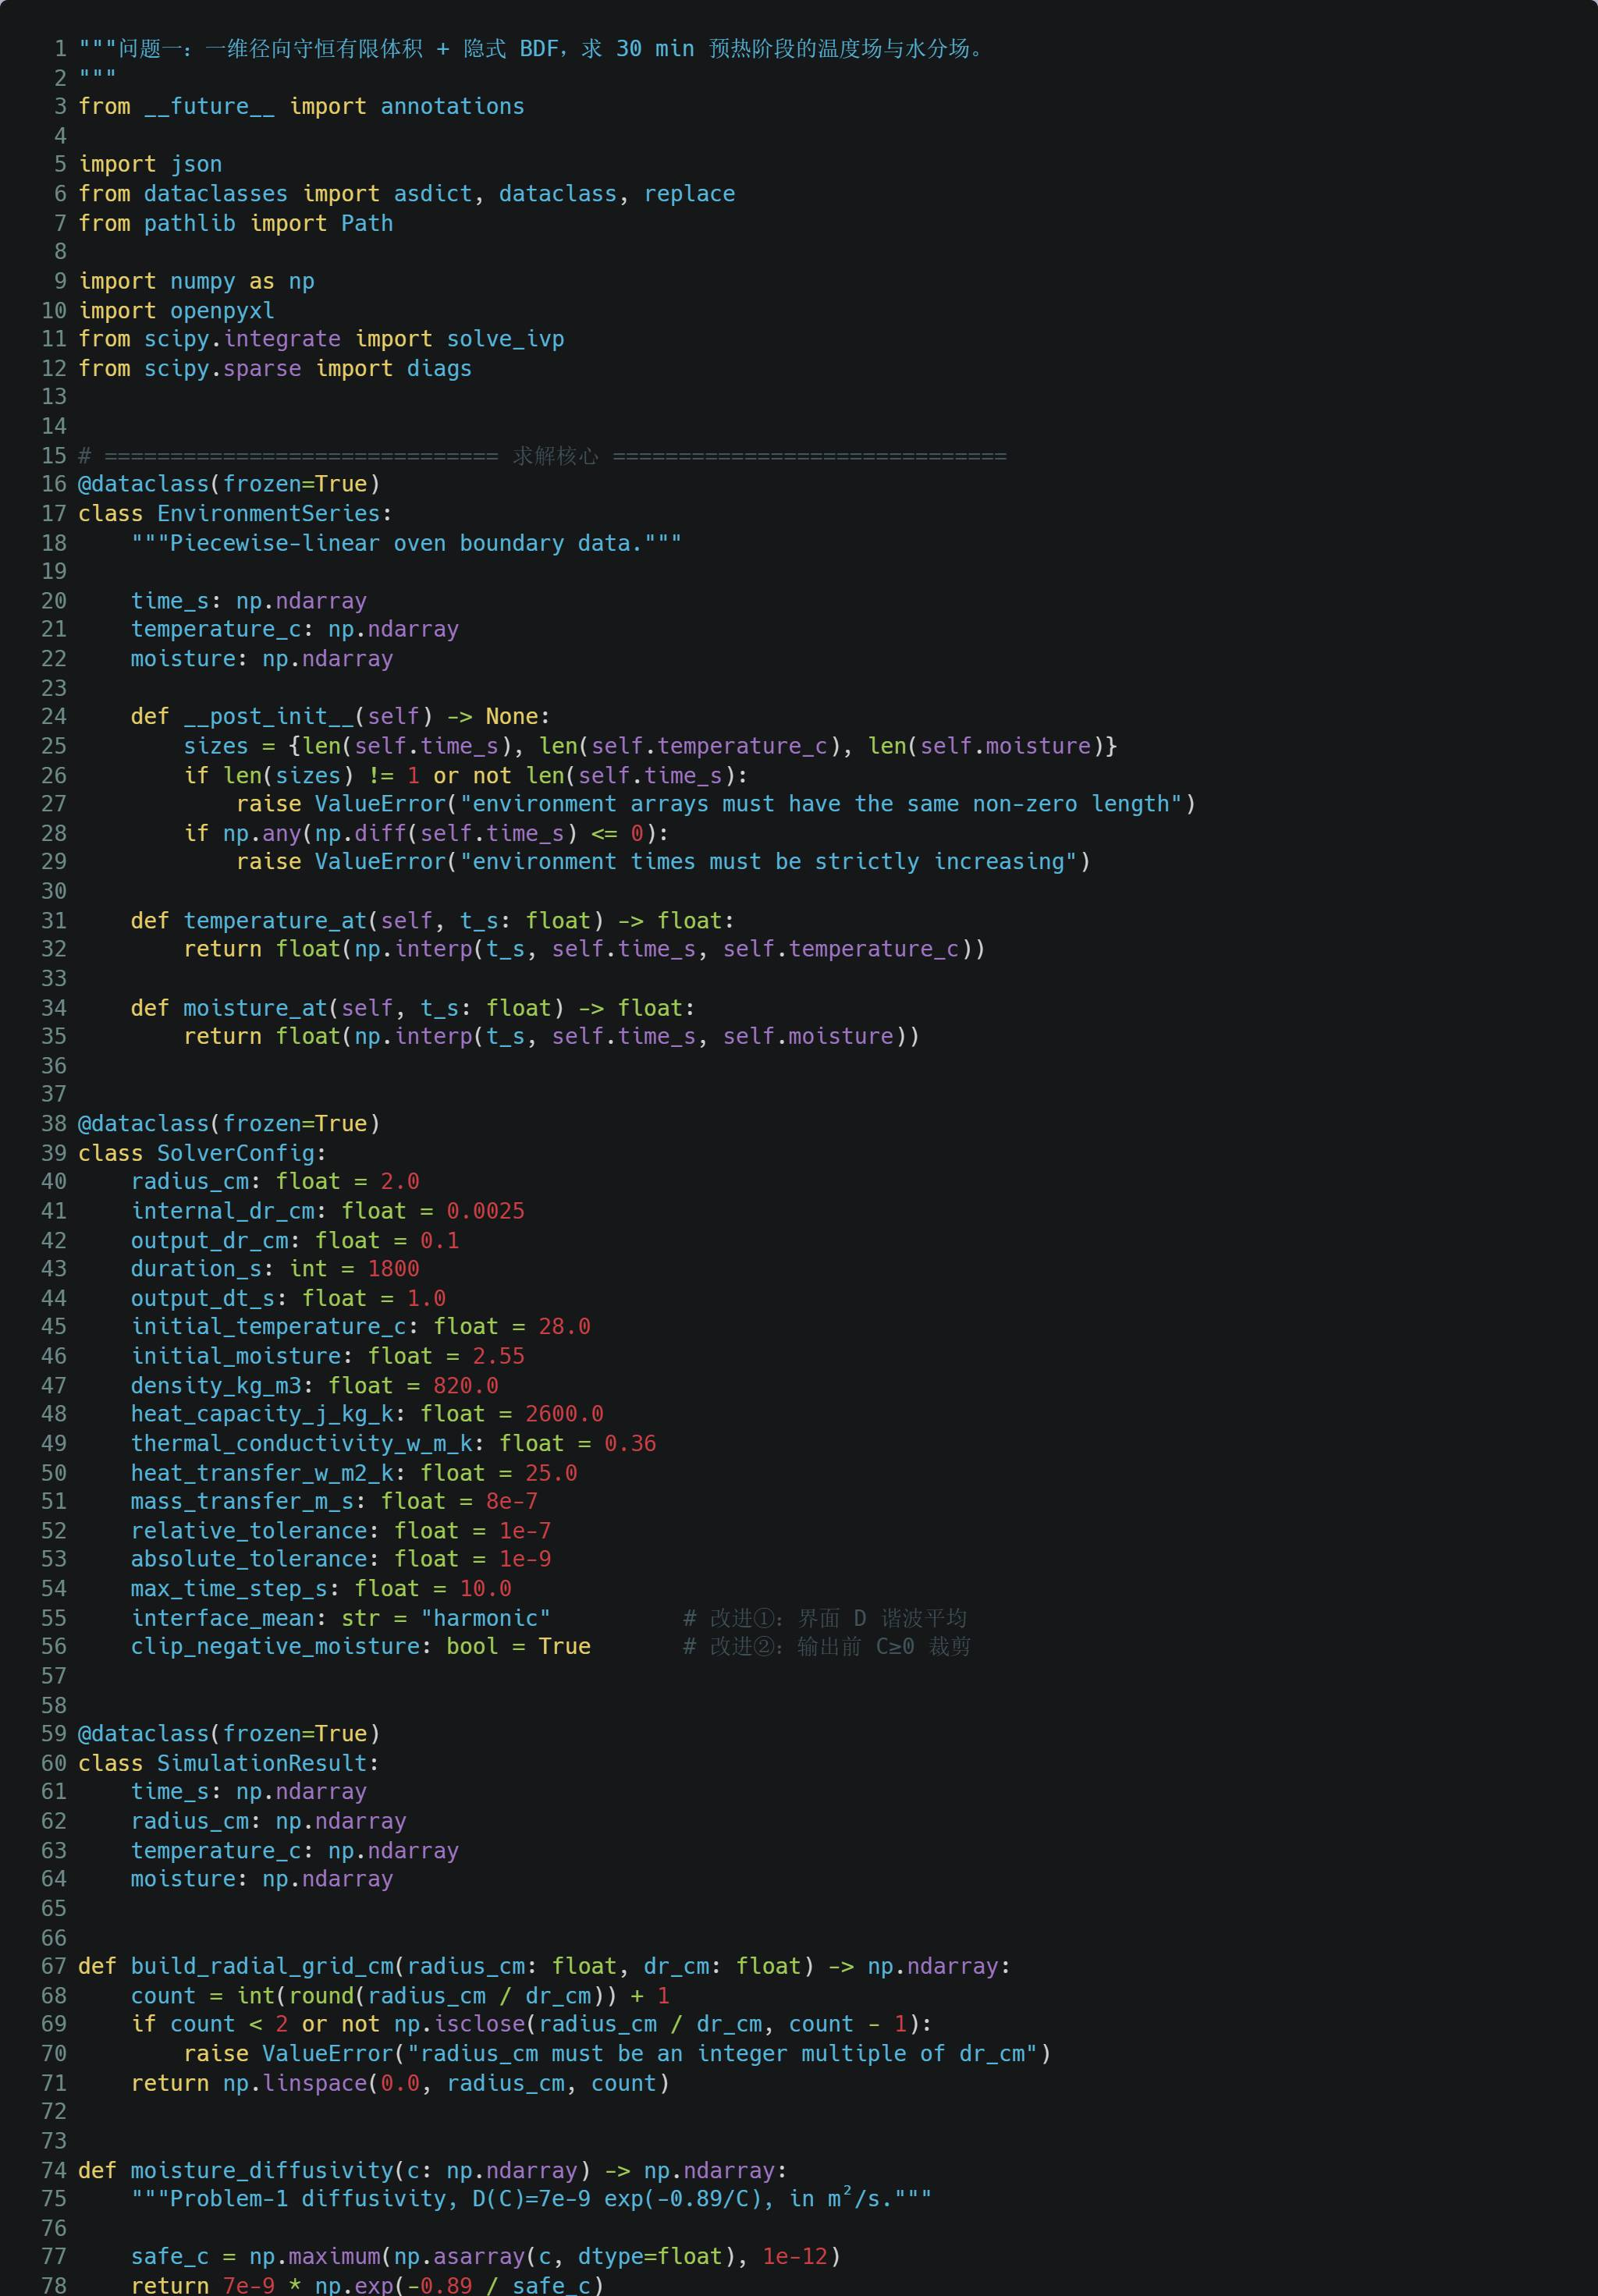
\includegraphics[width=\dimexpr\textwidth-24pt\relax]{../../code/submission/code_images/split/problem1_p1.jpg}
\newpage
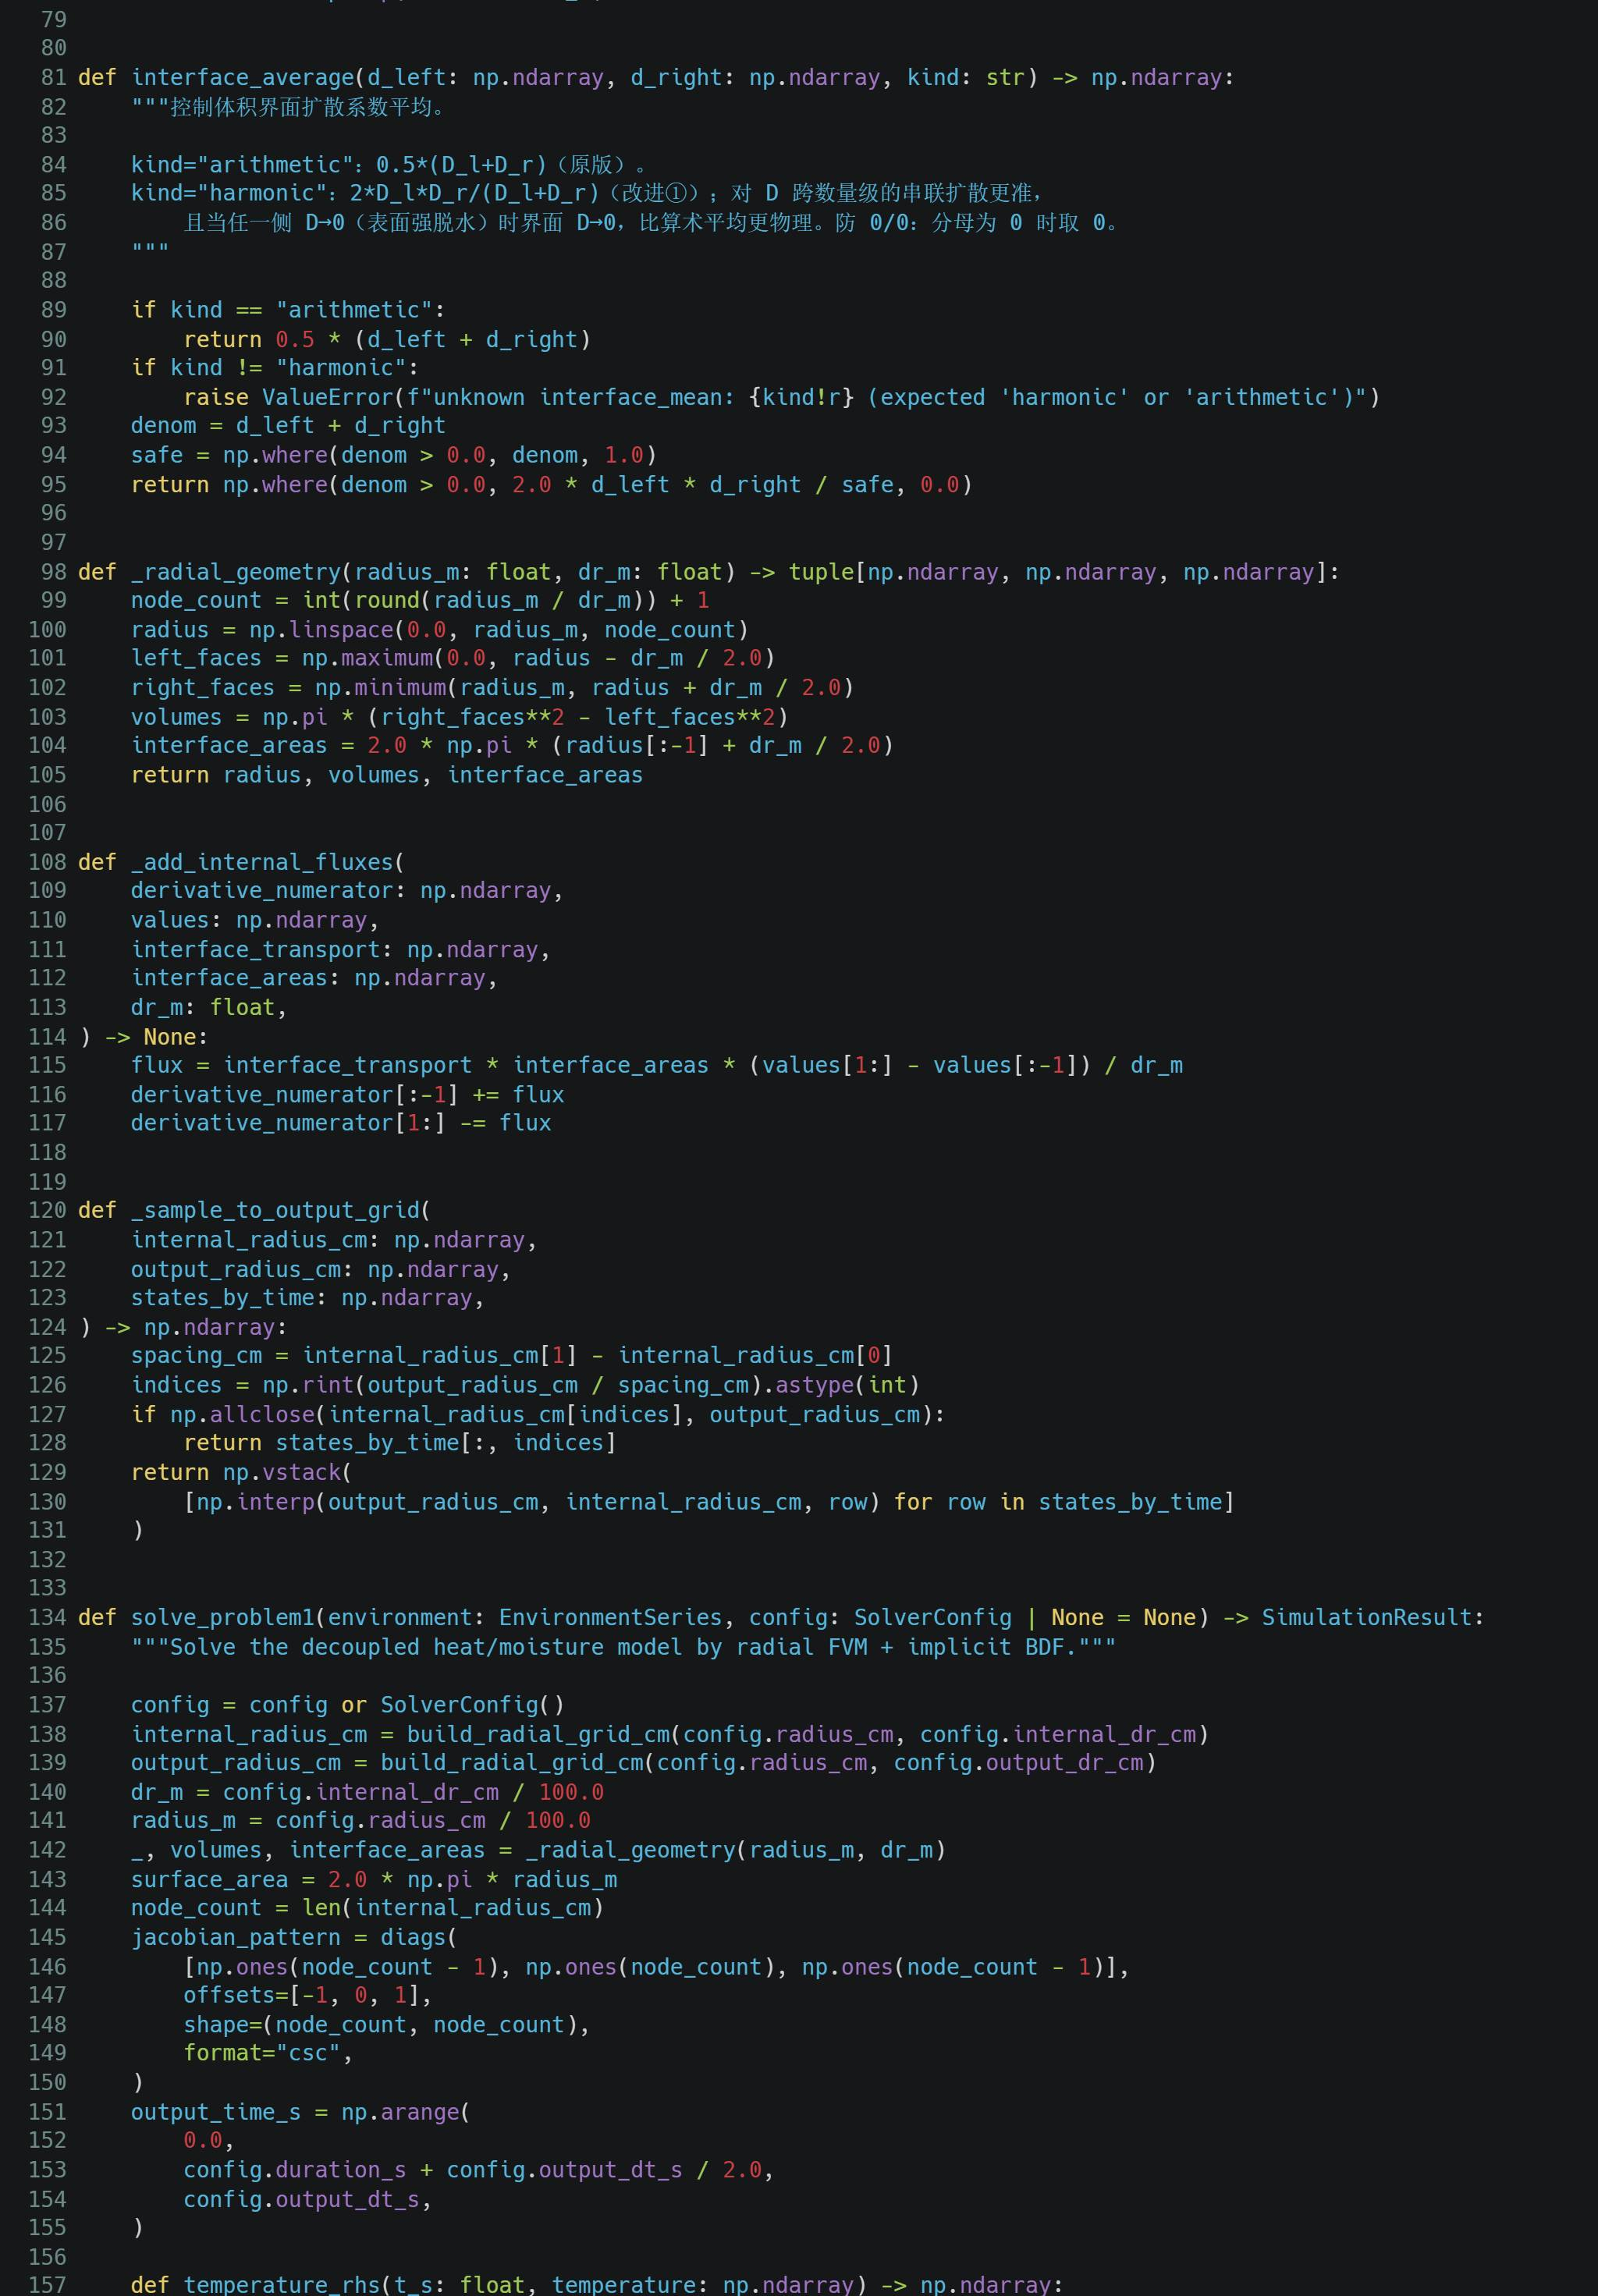
\includegraphics[width=\dimexpr\textwidth-24pt\relax]{../../code/submission/code_images/split/problem1_p2.jpg}
\newpage
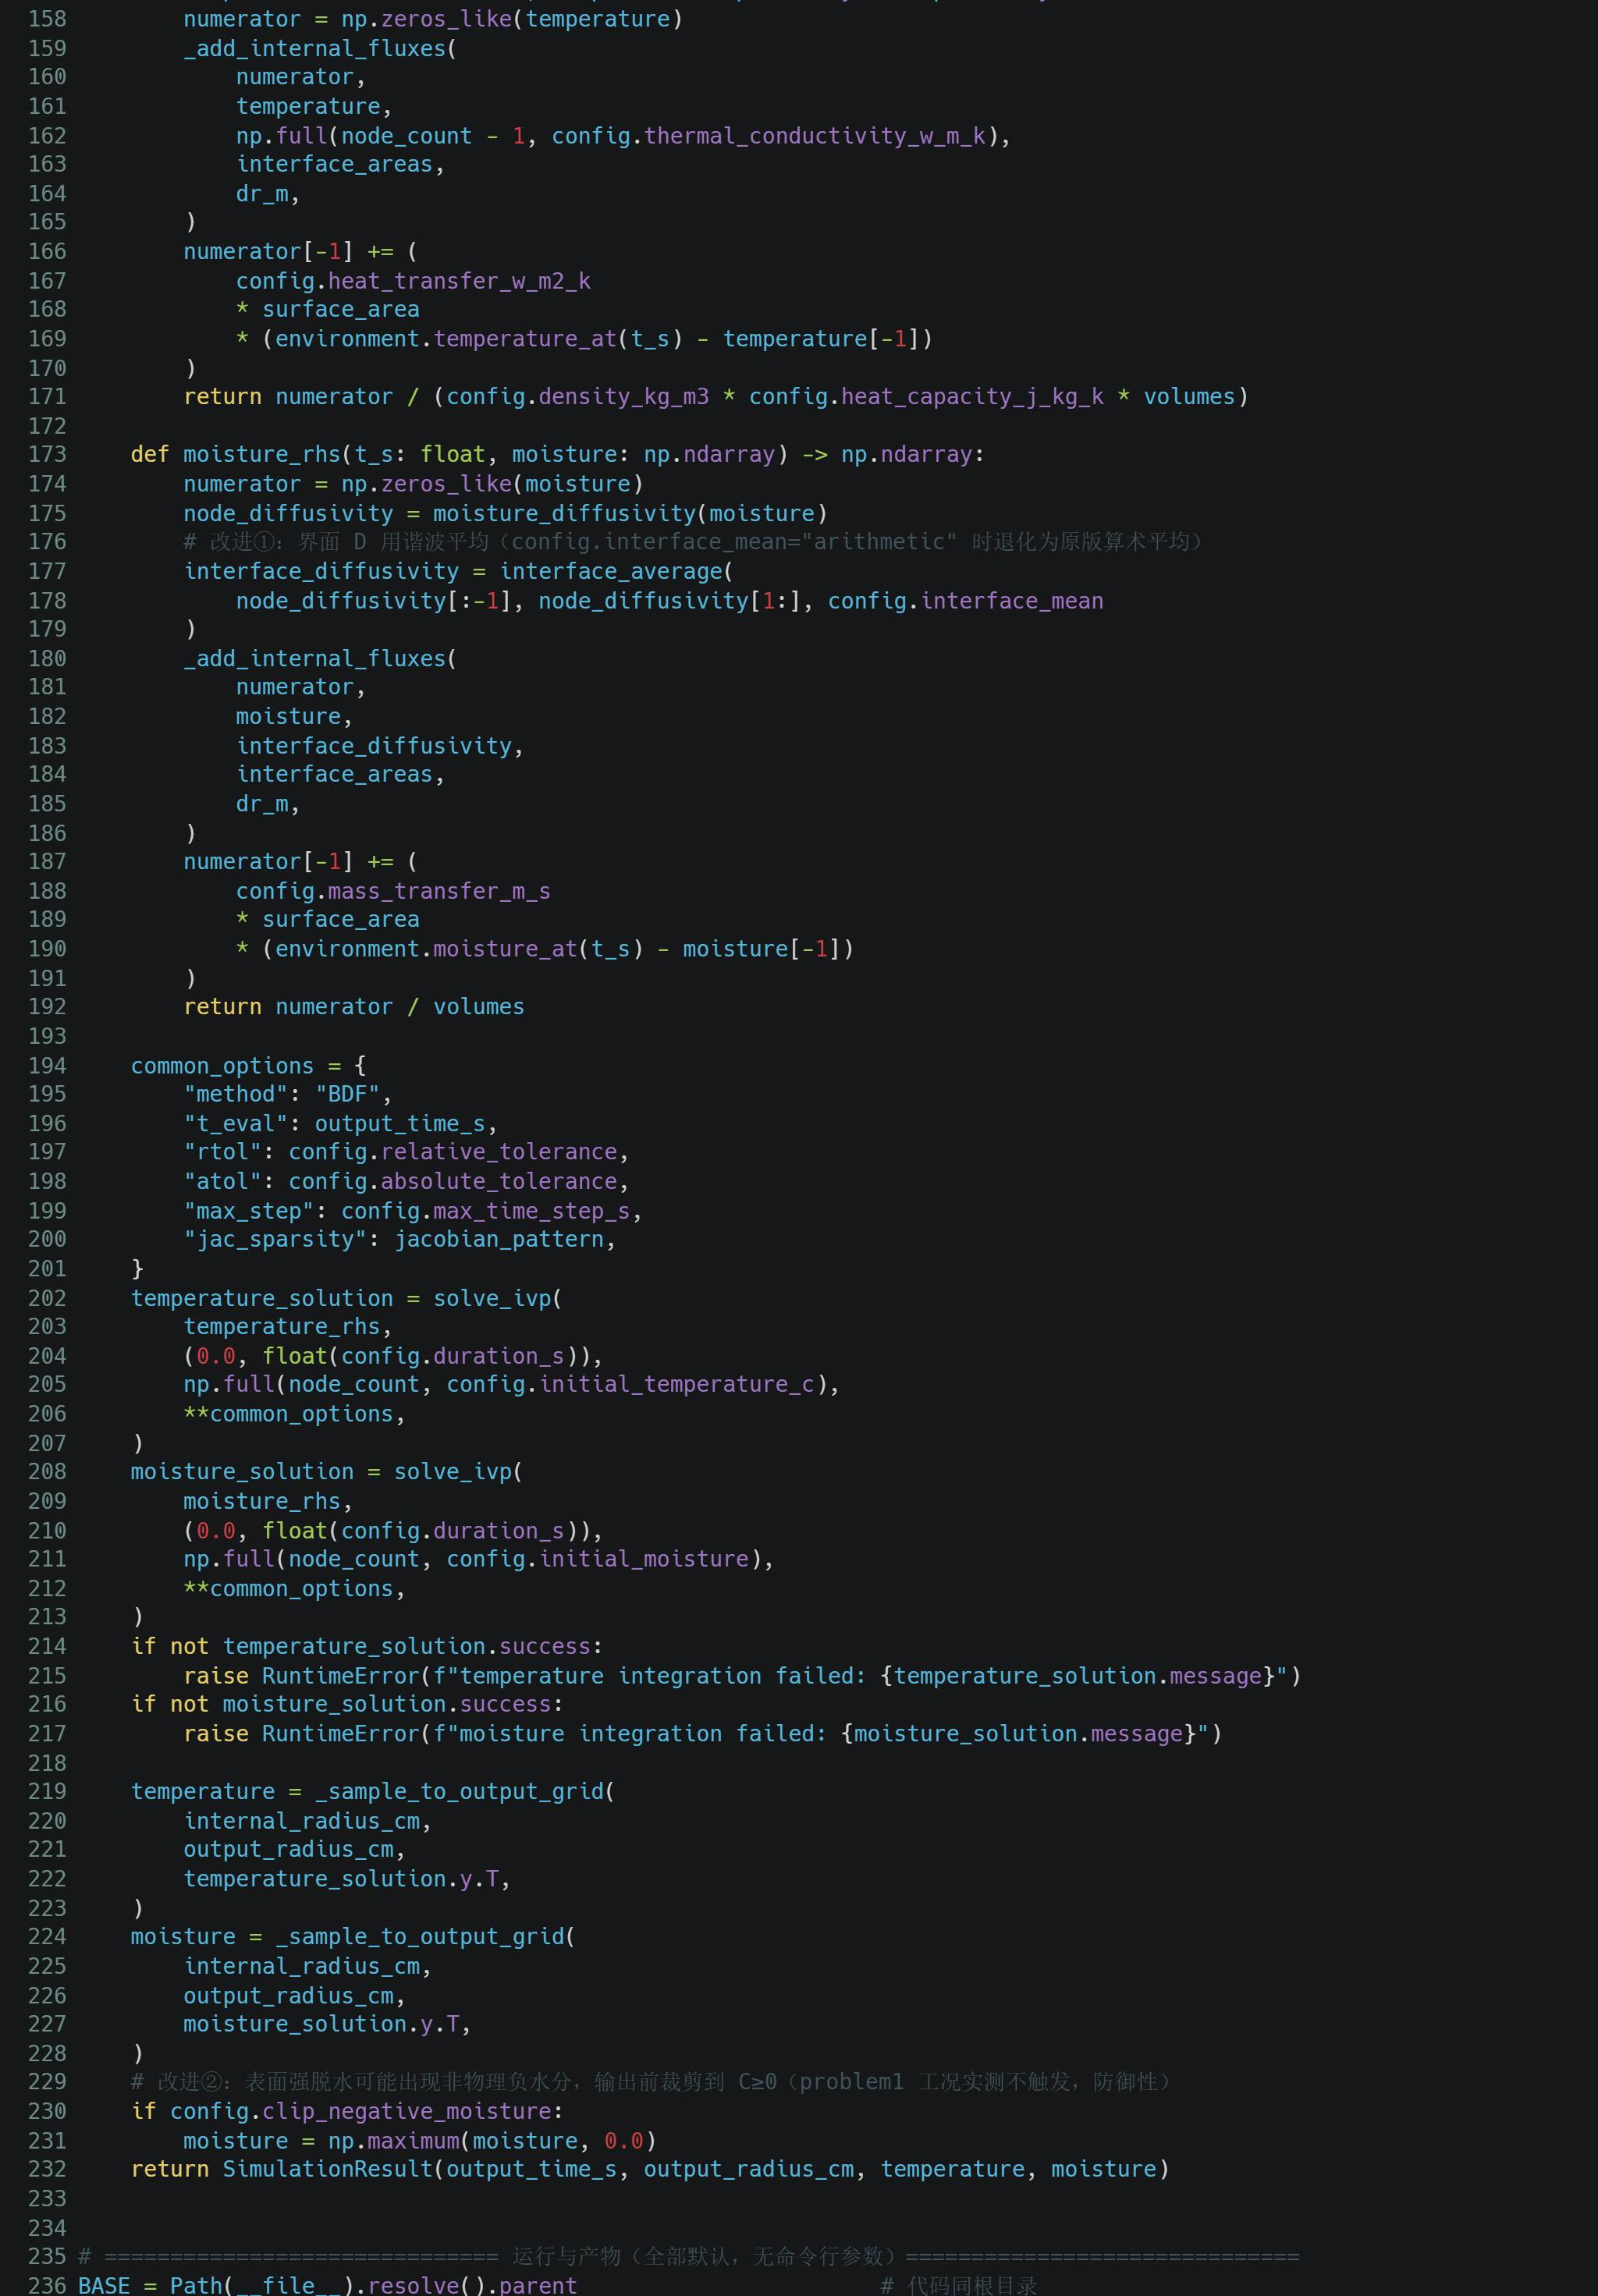
\includegraphics[width=\dimexpr\textwidth-24pt\relax]{../../code/submission/code_images/split/problem1_p3.jpg}
\newpage
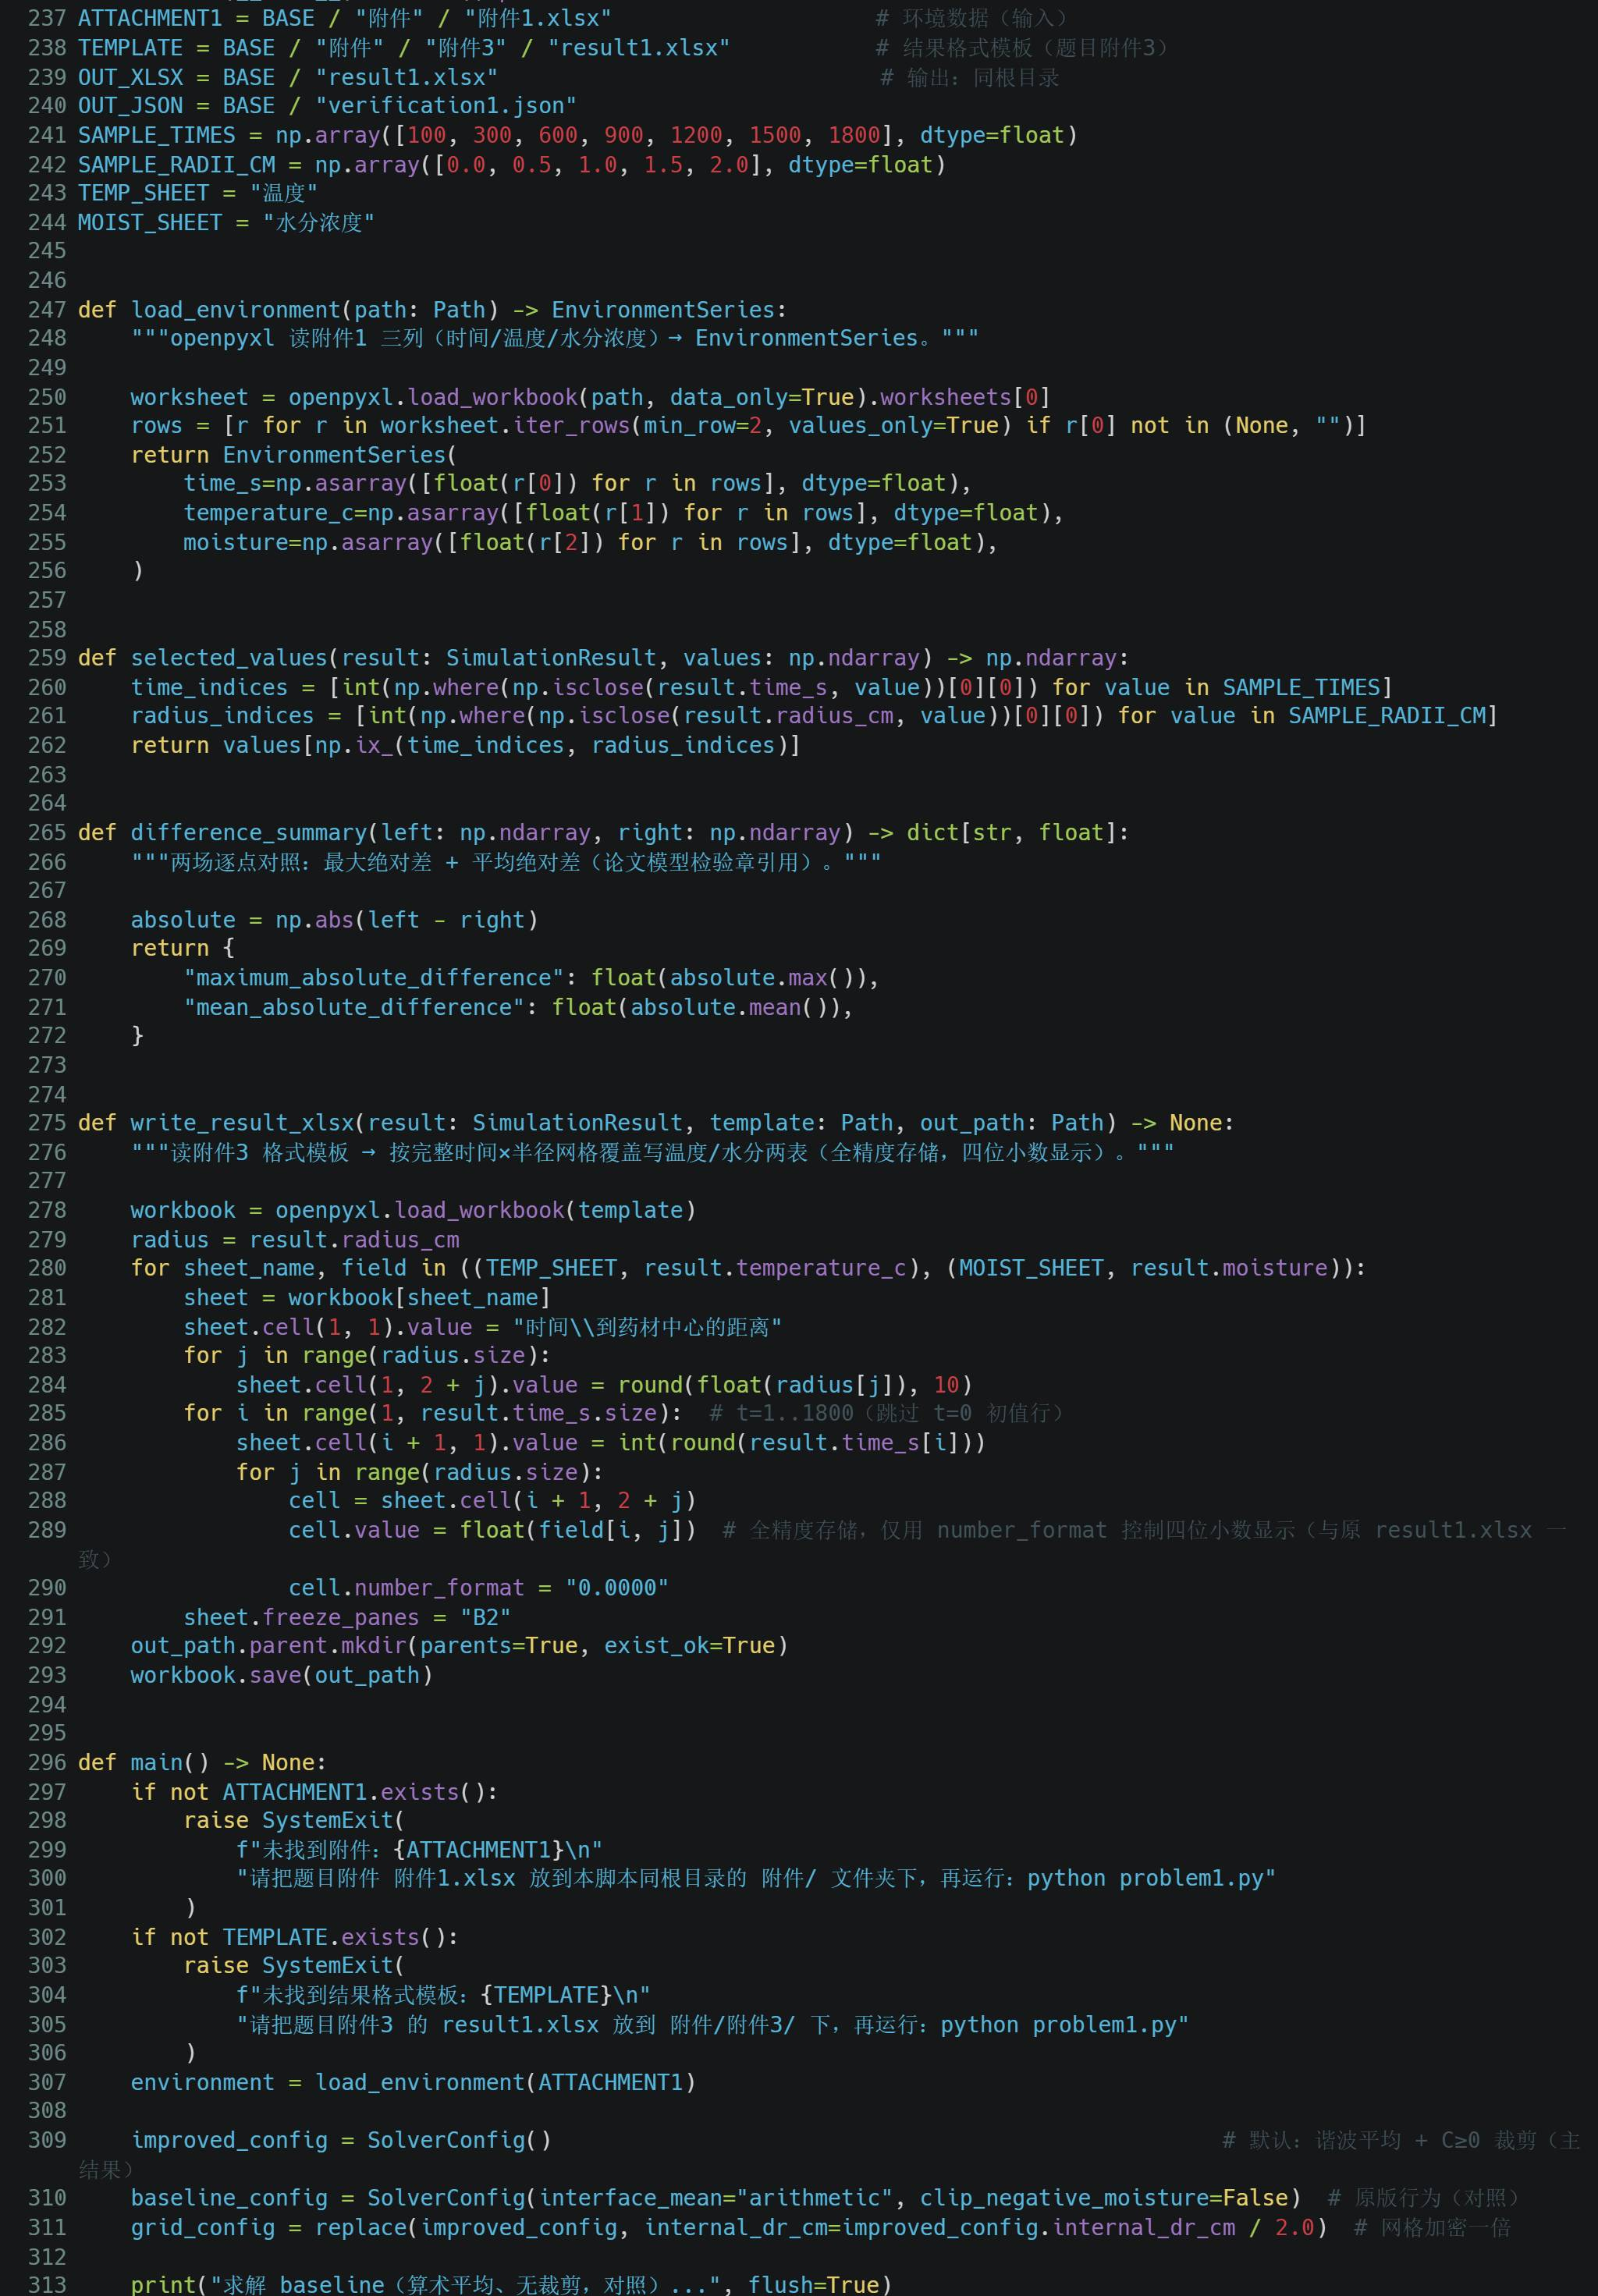
\includegraphics[width=\dimexpr\textwidth-24pt\relax]{../../code/submission/code_images/split/problem1_p4.jpg}
\newpage
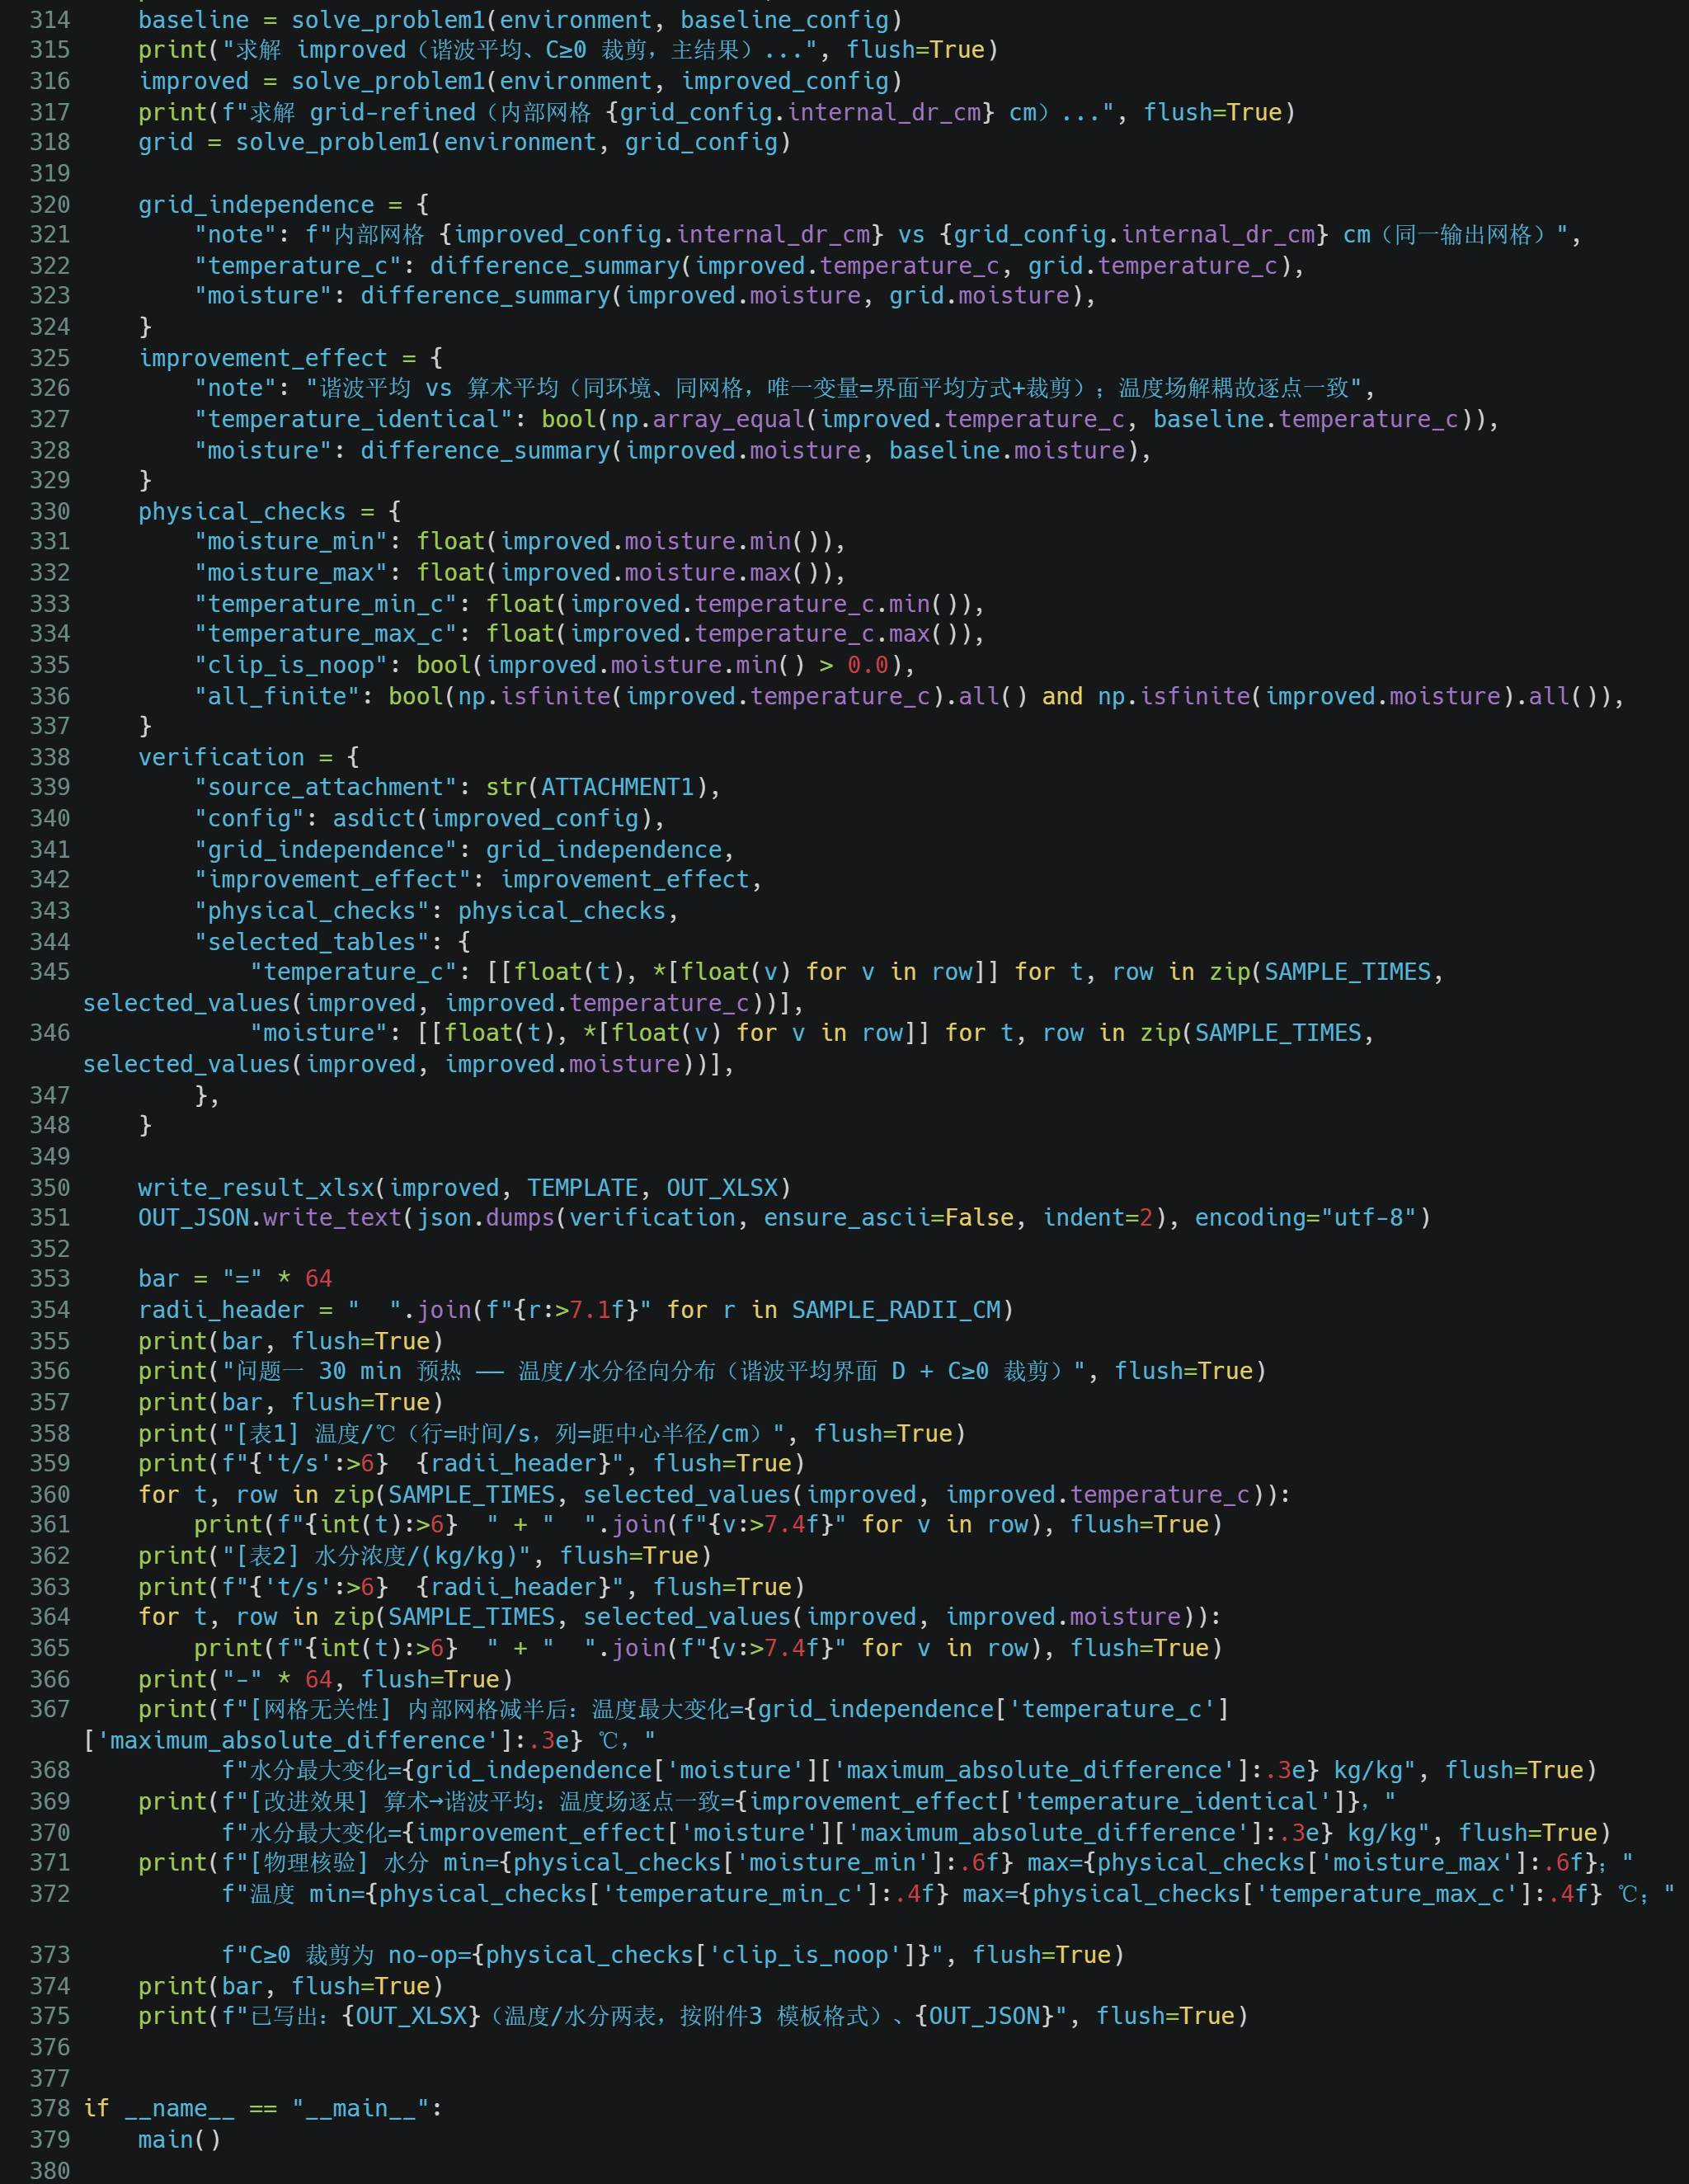
\includegraphics[width=\dimexpr\textwidth-24pt\relax]{../../code/submission/code_images/split/problem1_p5.jpg}
\newpage
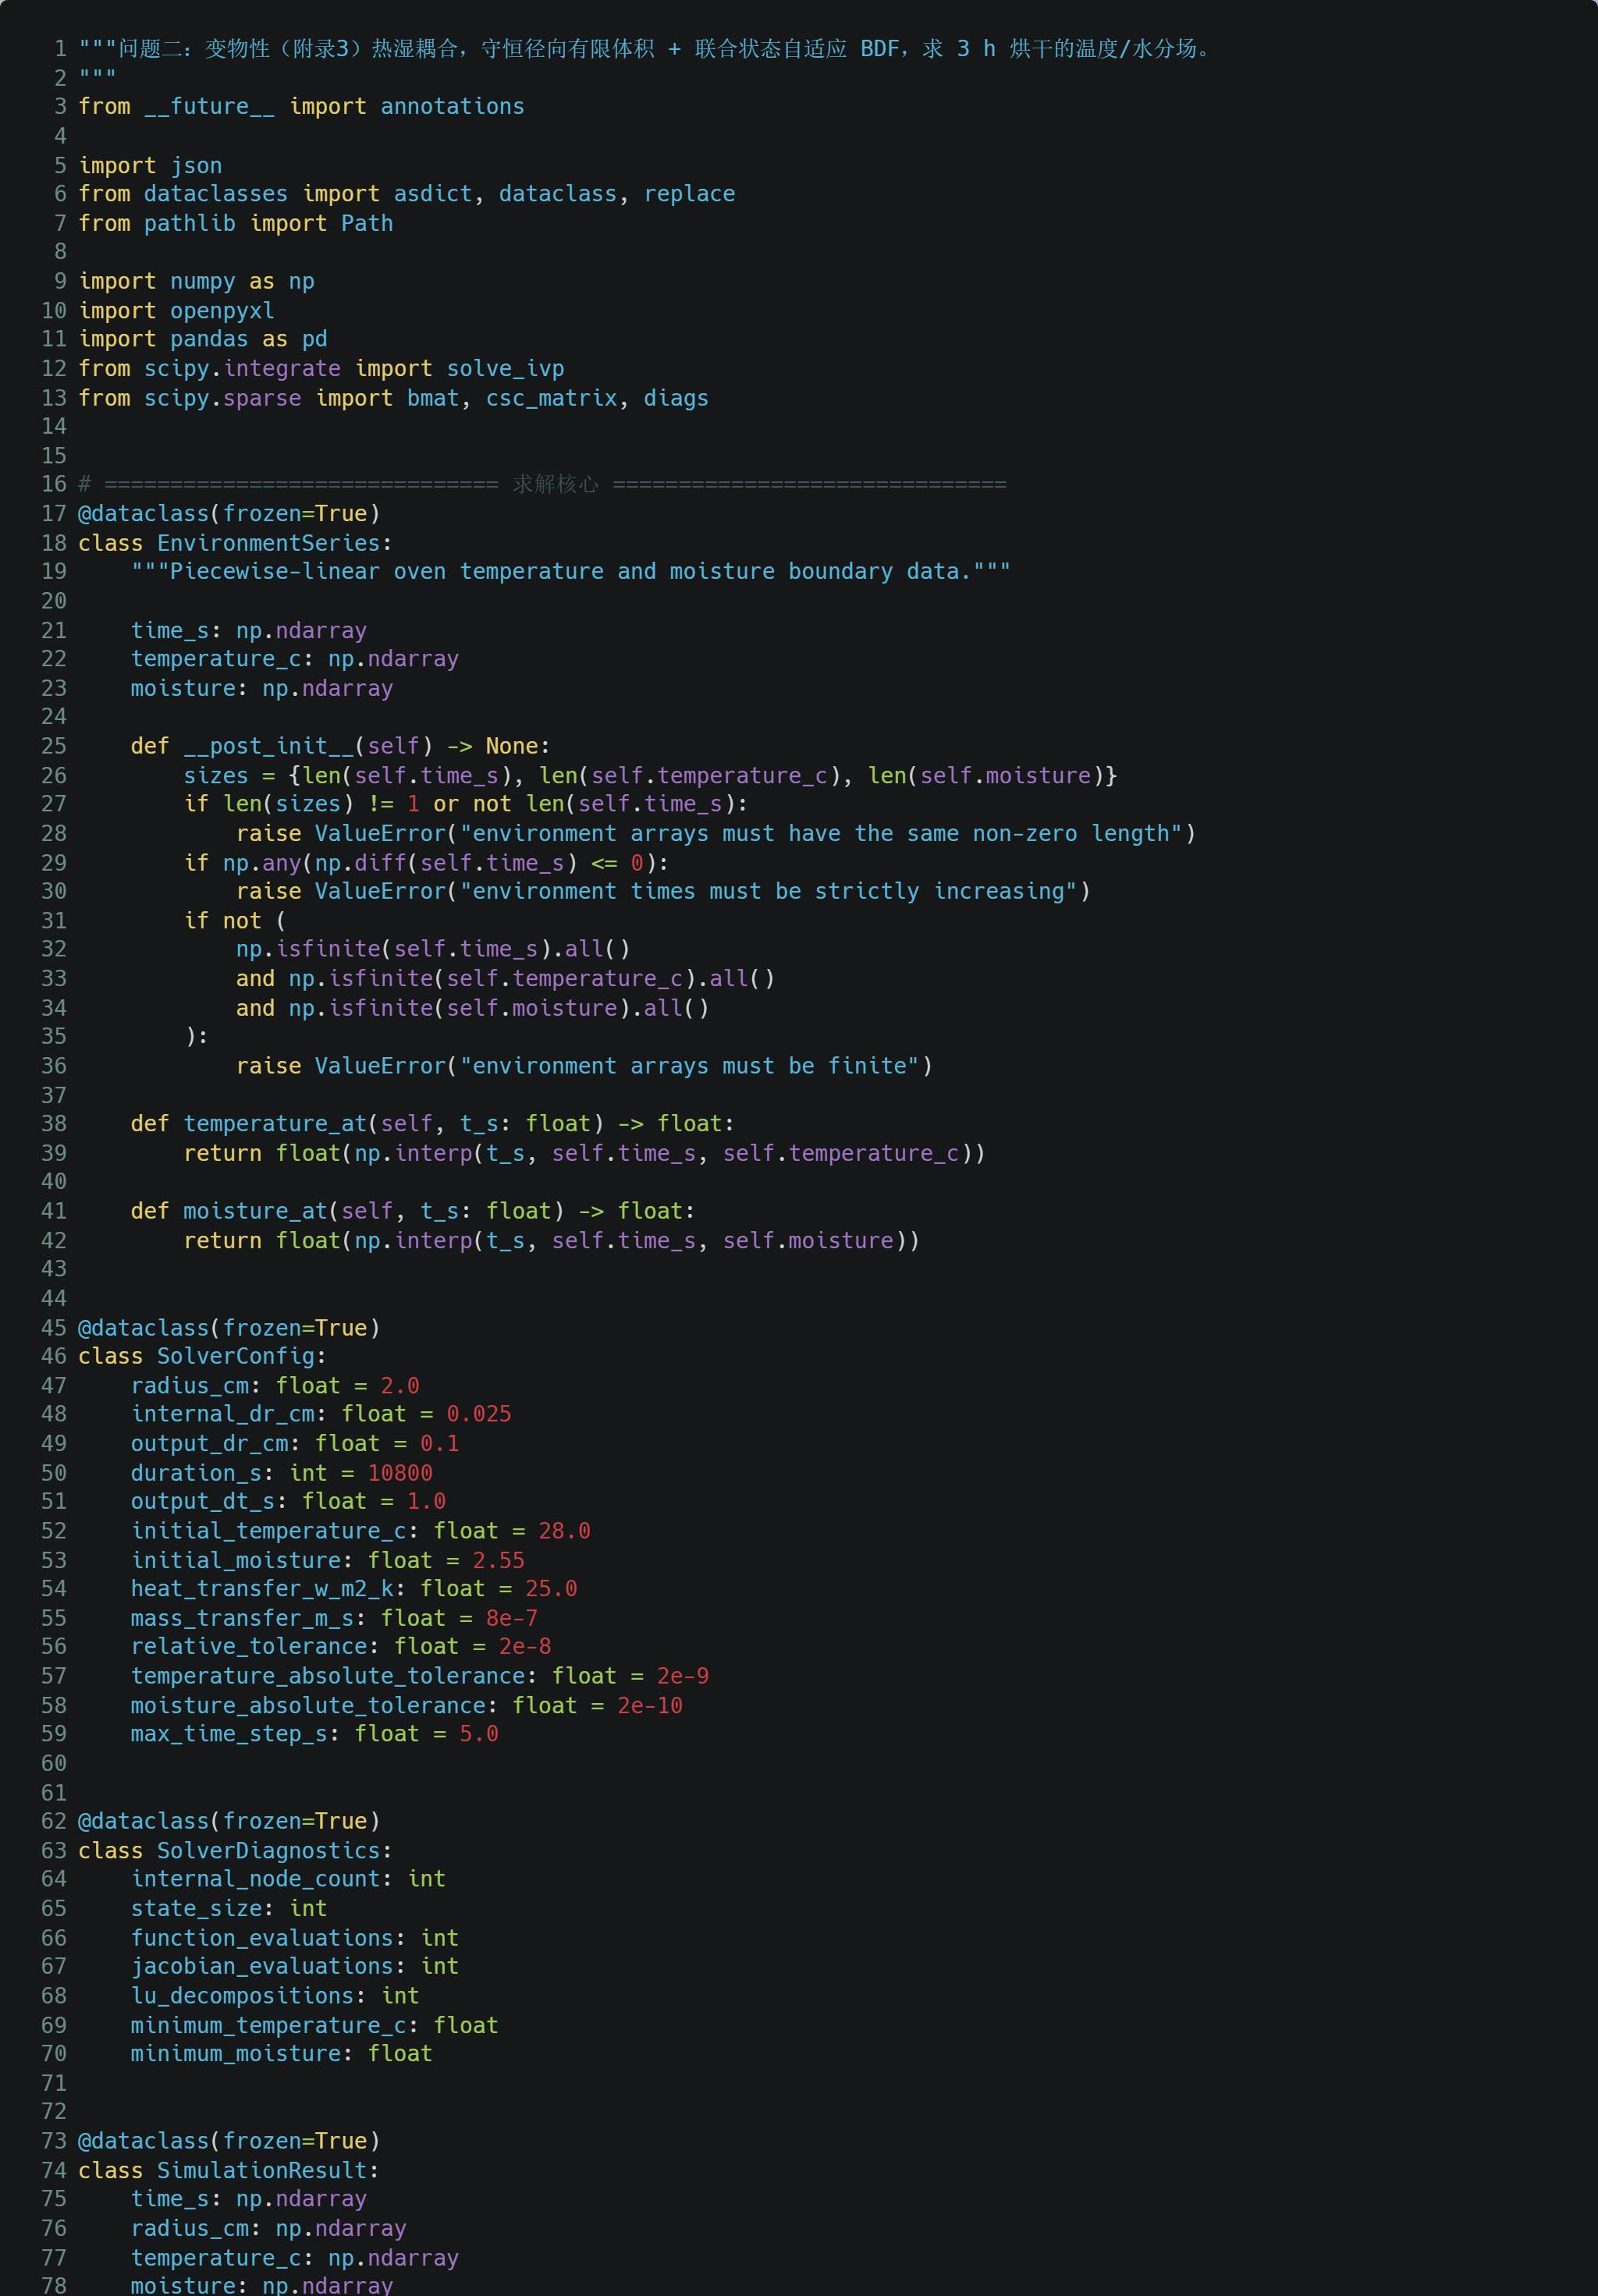
\includegraphics[width=\dimexpr\textwidth-24pt\relax]{../../code/submission/code_images/split/problem2_p1.jpg}
\newpage
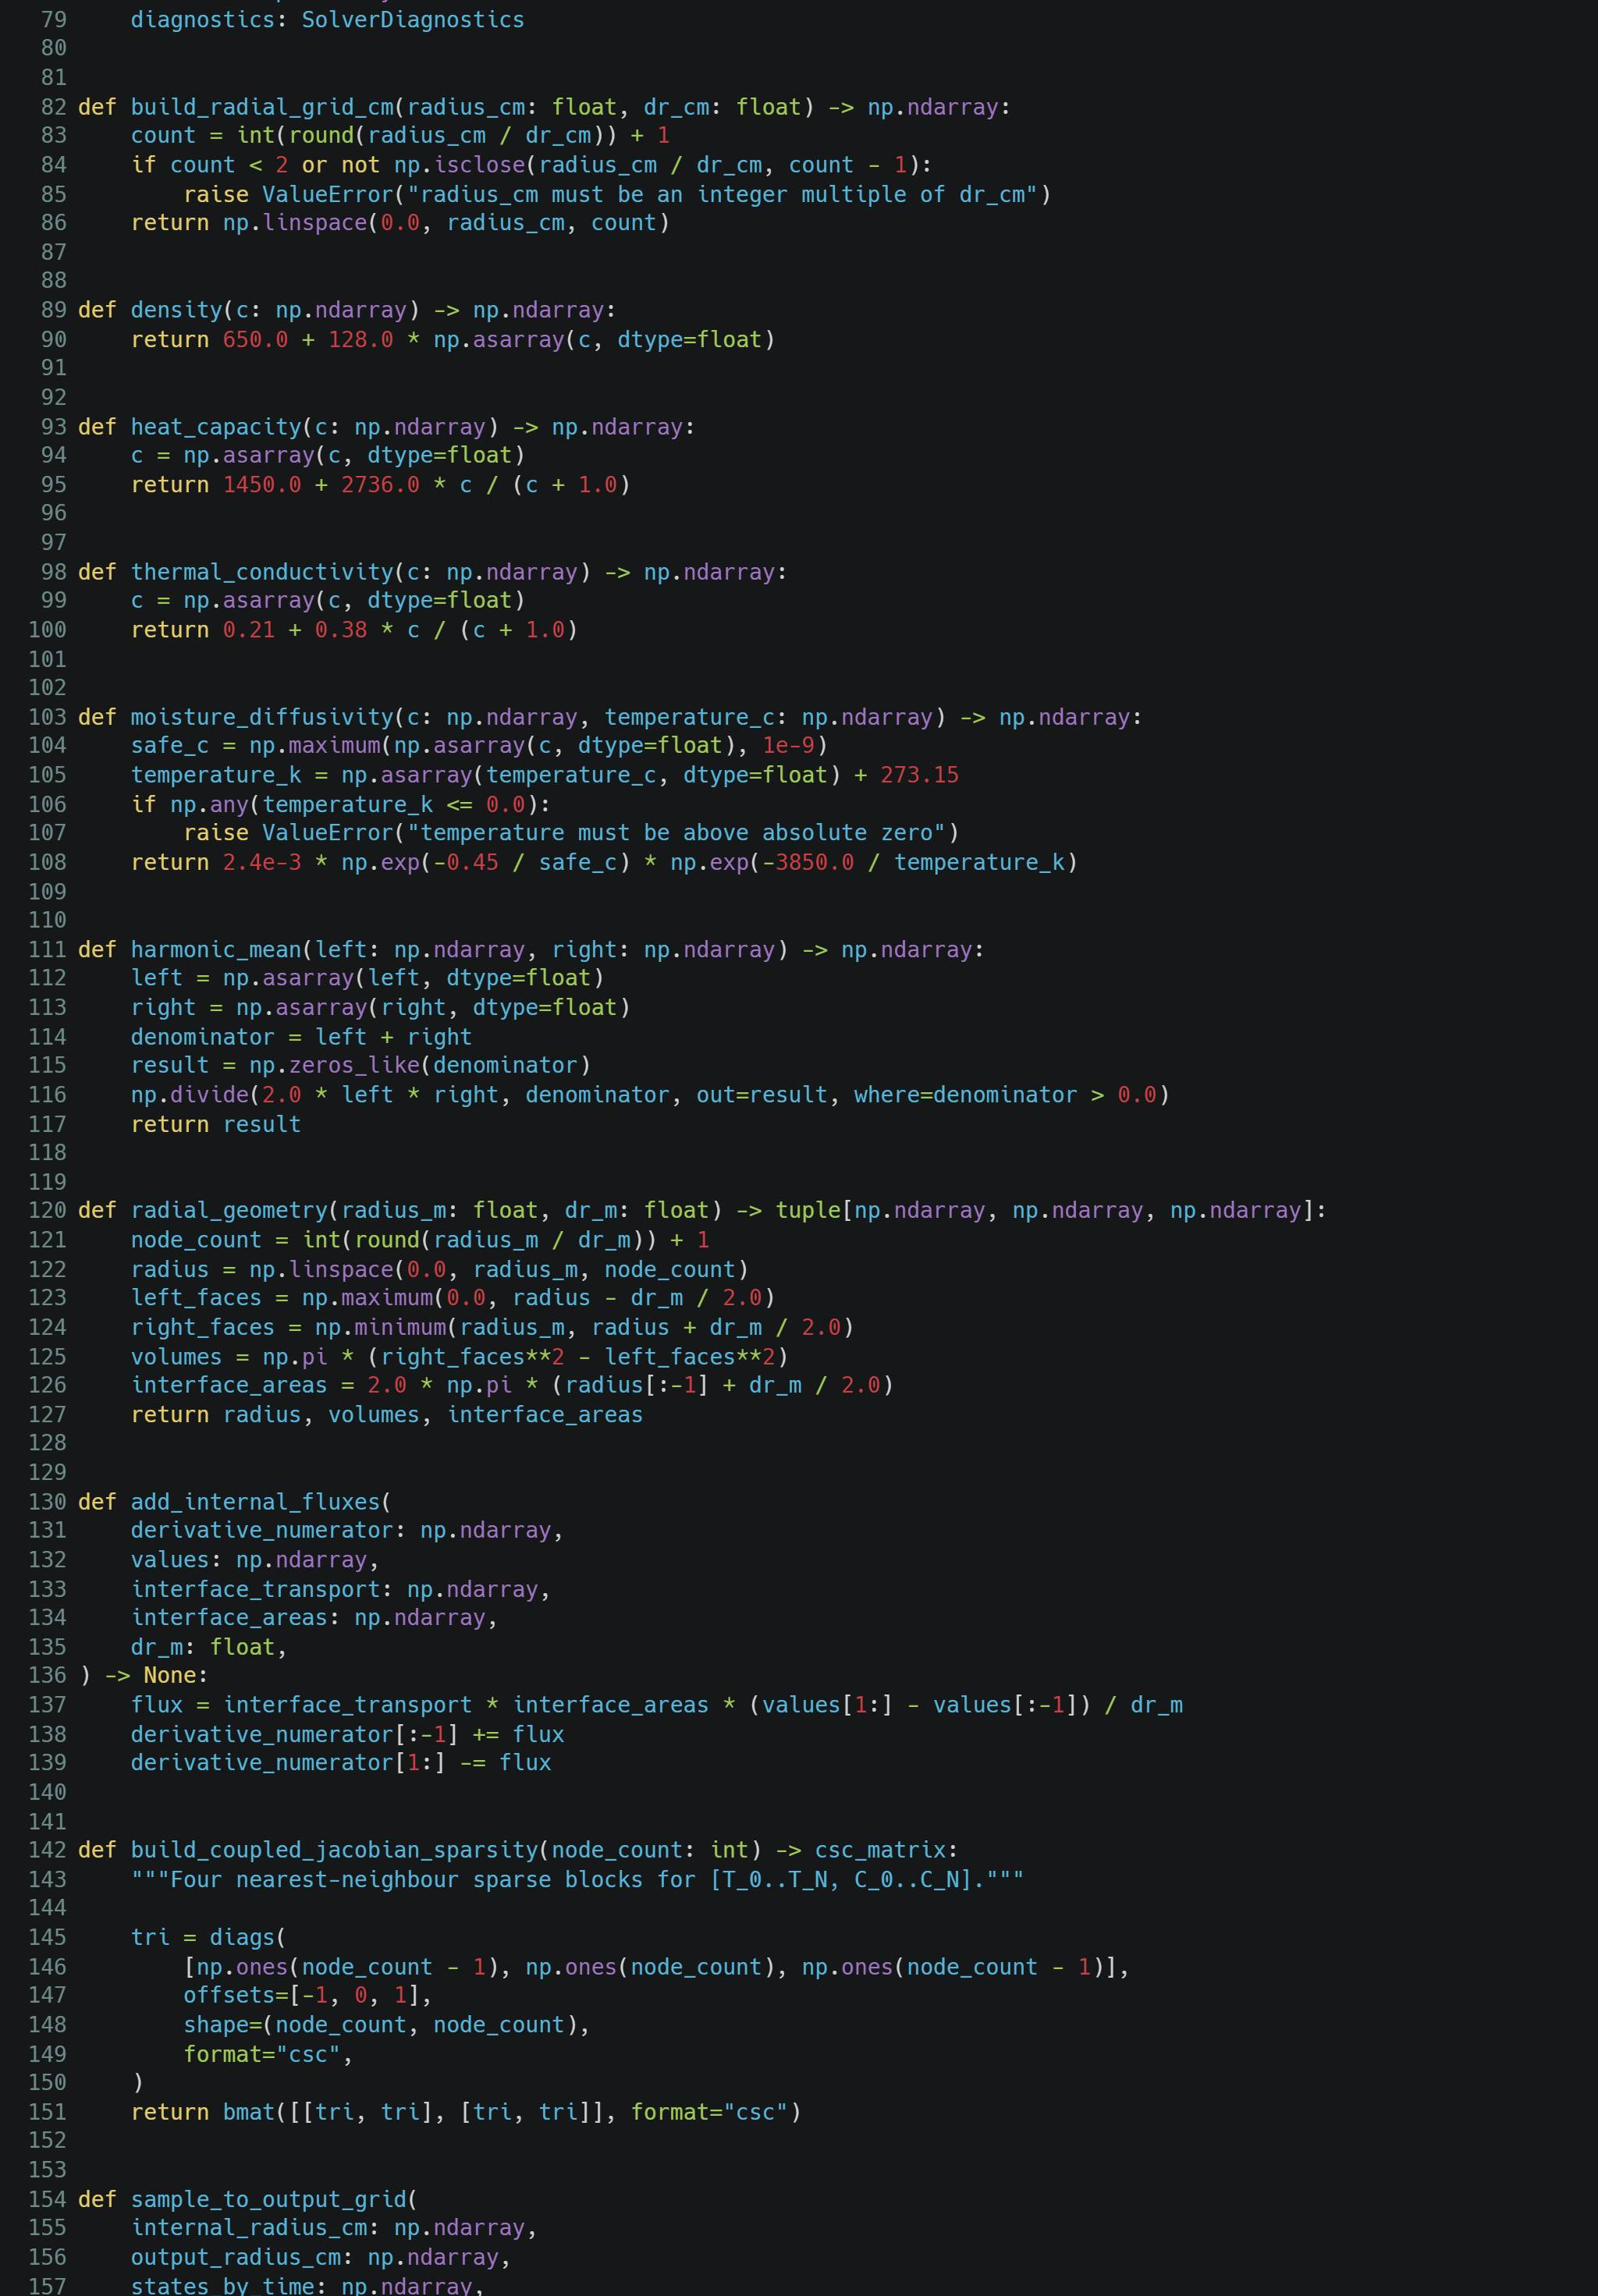
\includegraphics[width=\dimexpr\textwidth-24pt\relax]{../../code/submission/code_images/split/problem2_p2.jpg}
\newpage
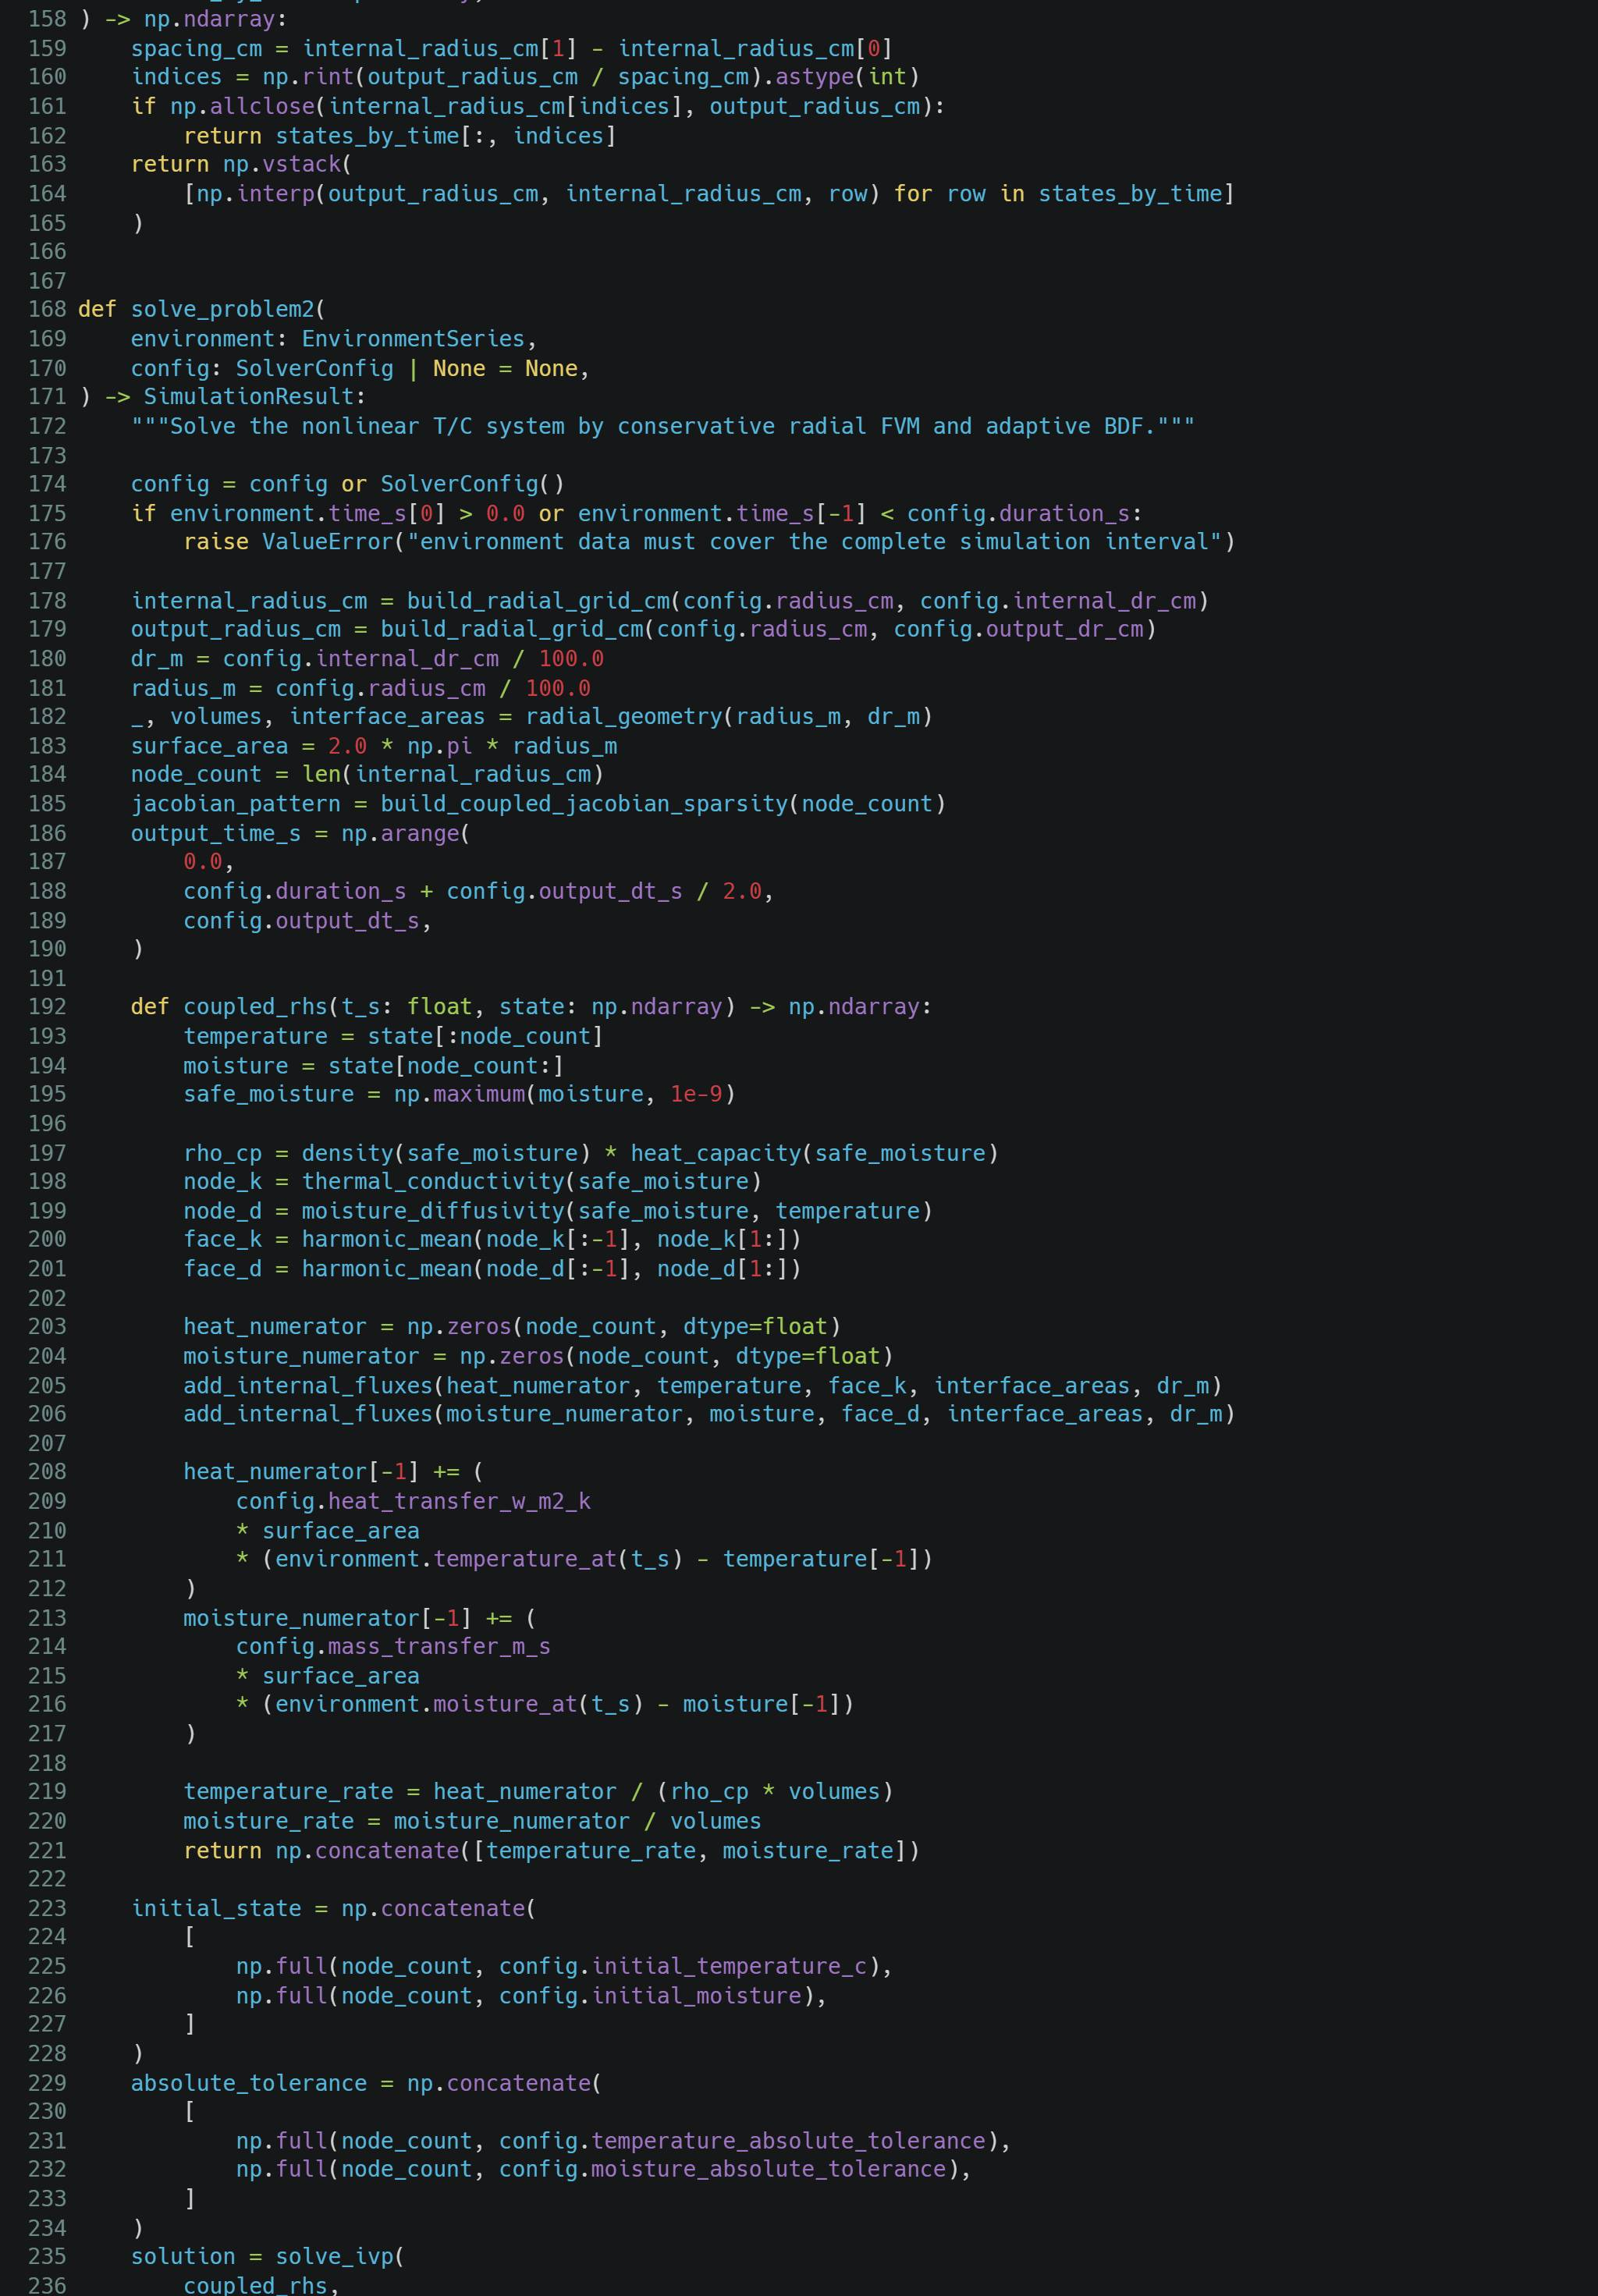
\includegraphics[width=\dimexpr\textwidth-24pt\relax]{../../code/submission/code_images/split/problem2_p3.jpg}
\newpage
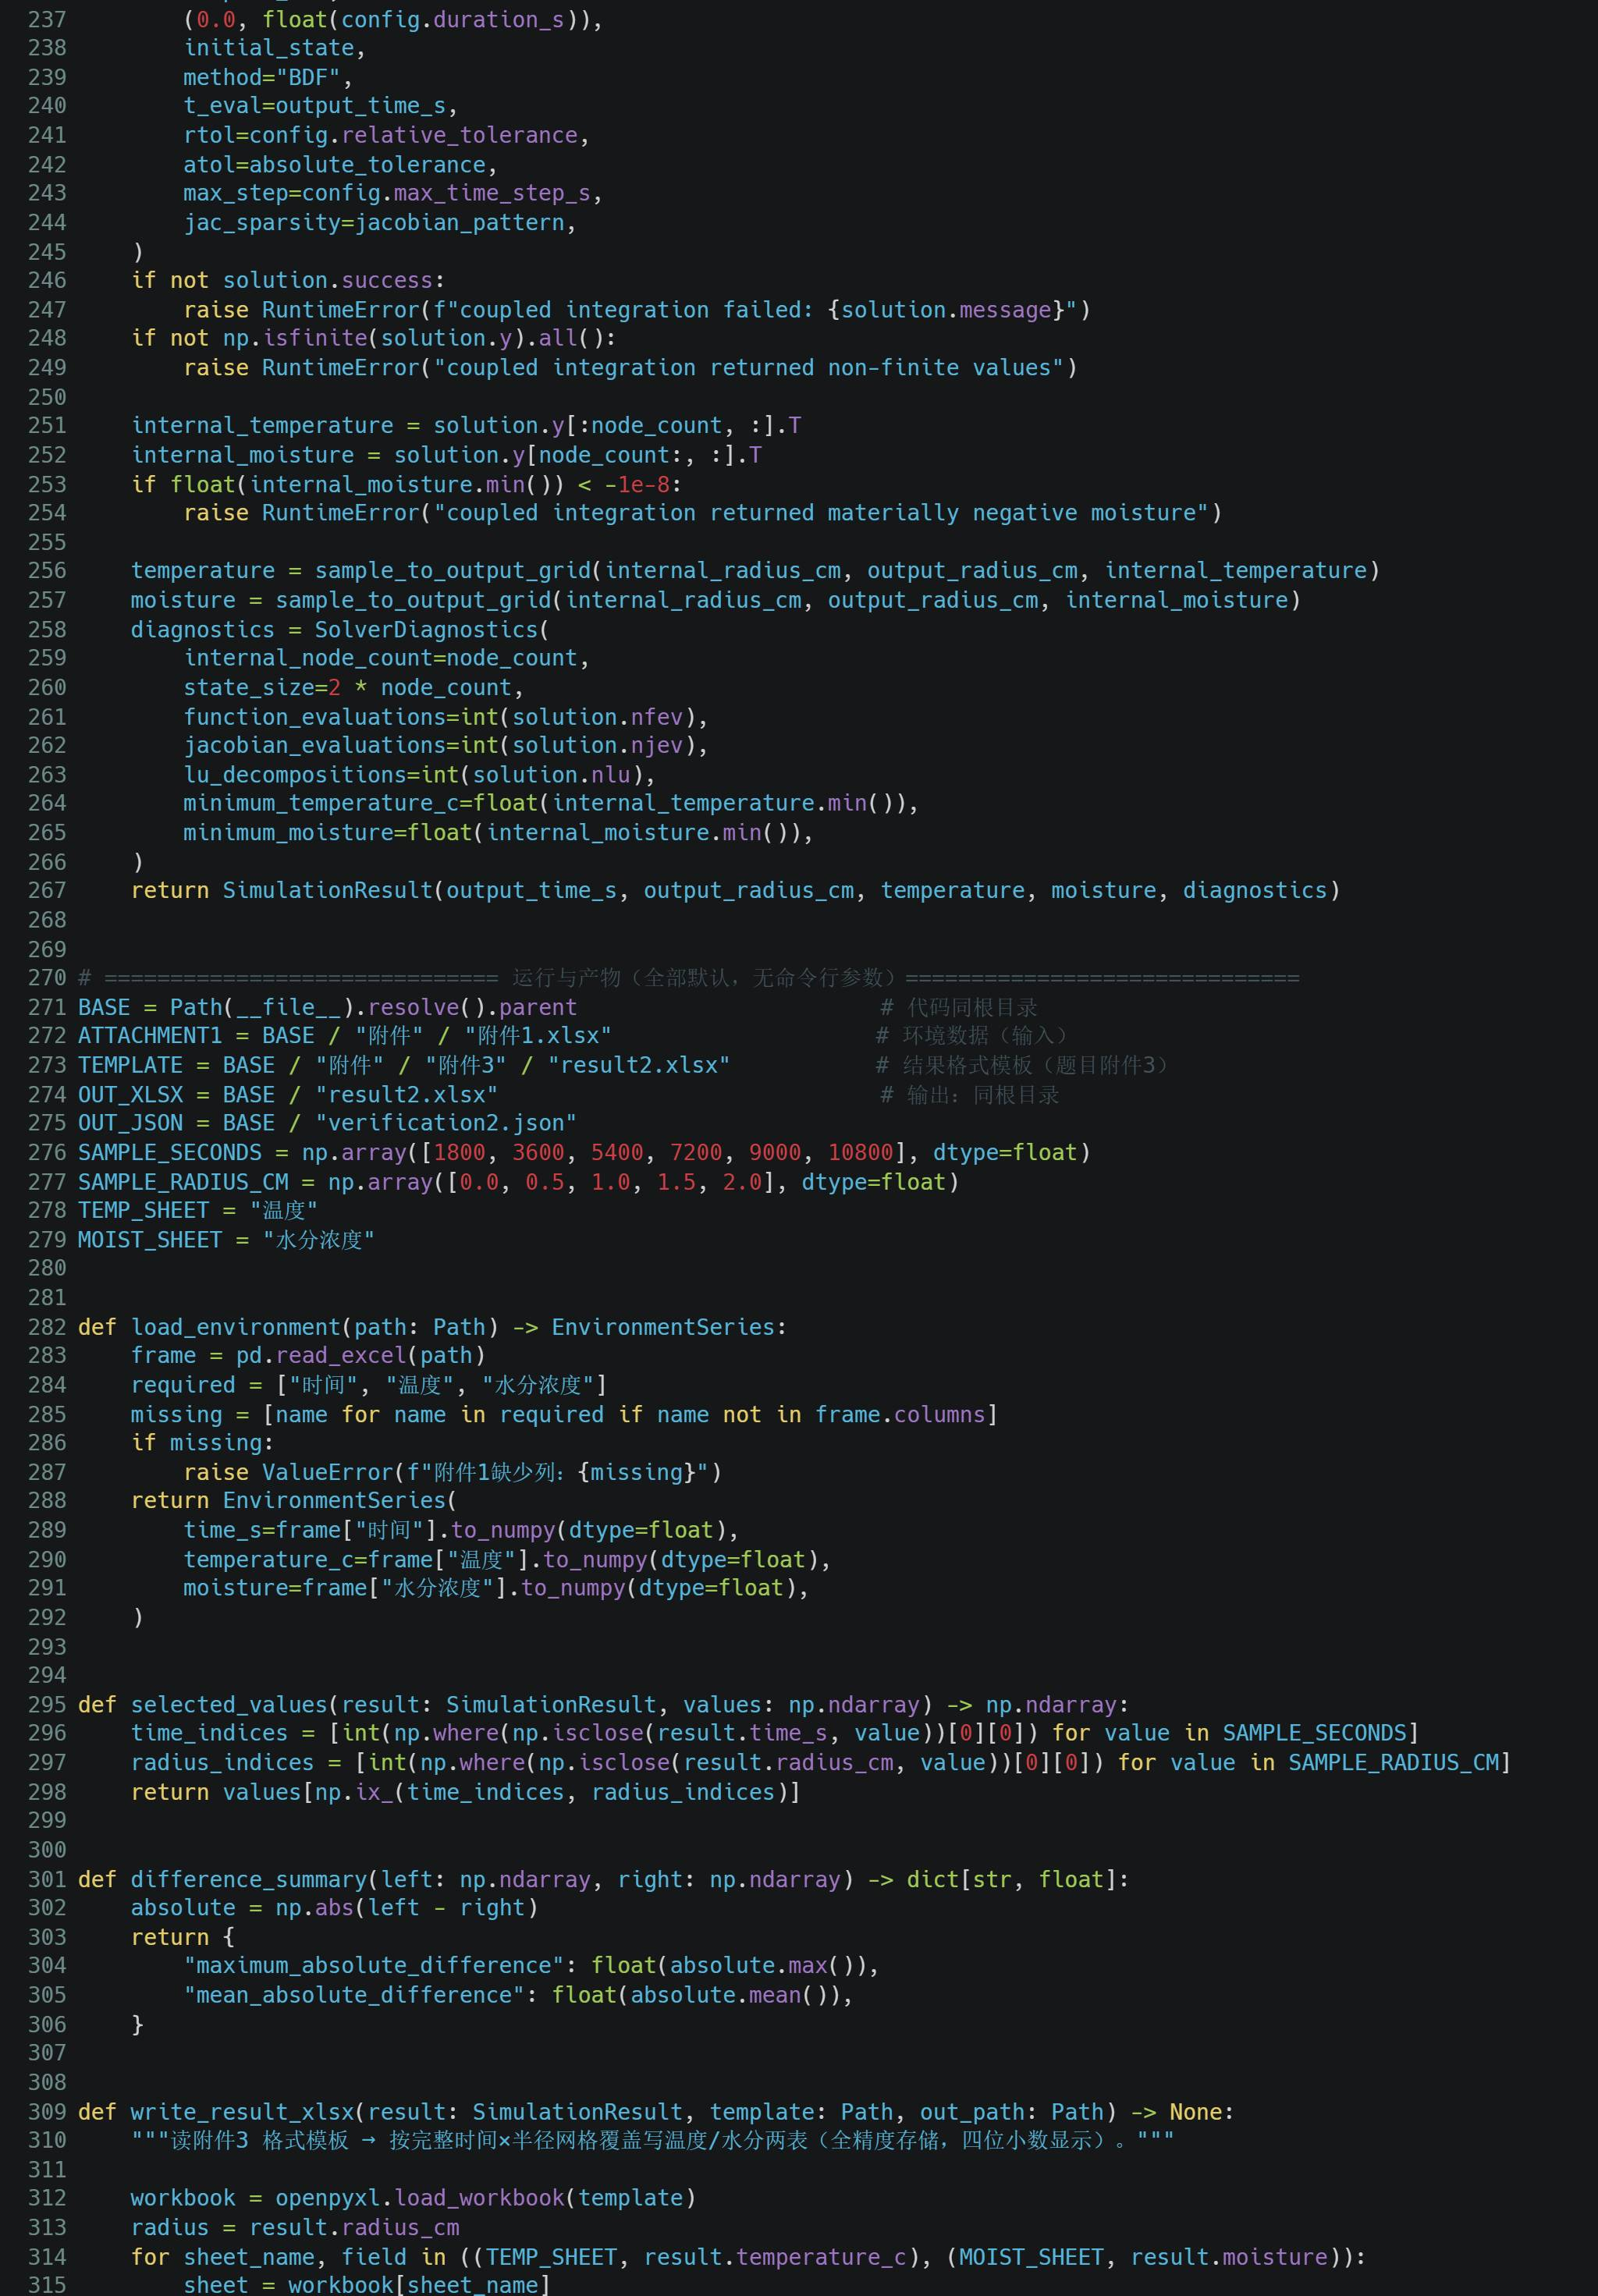
\includegraphics[width=\dimexpr\textwidth-24pt\relax]{../../code/submission/code_images/split/problem2_p4.jpg}
\newpage
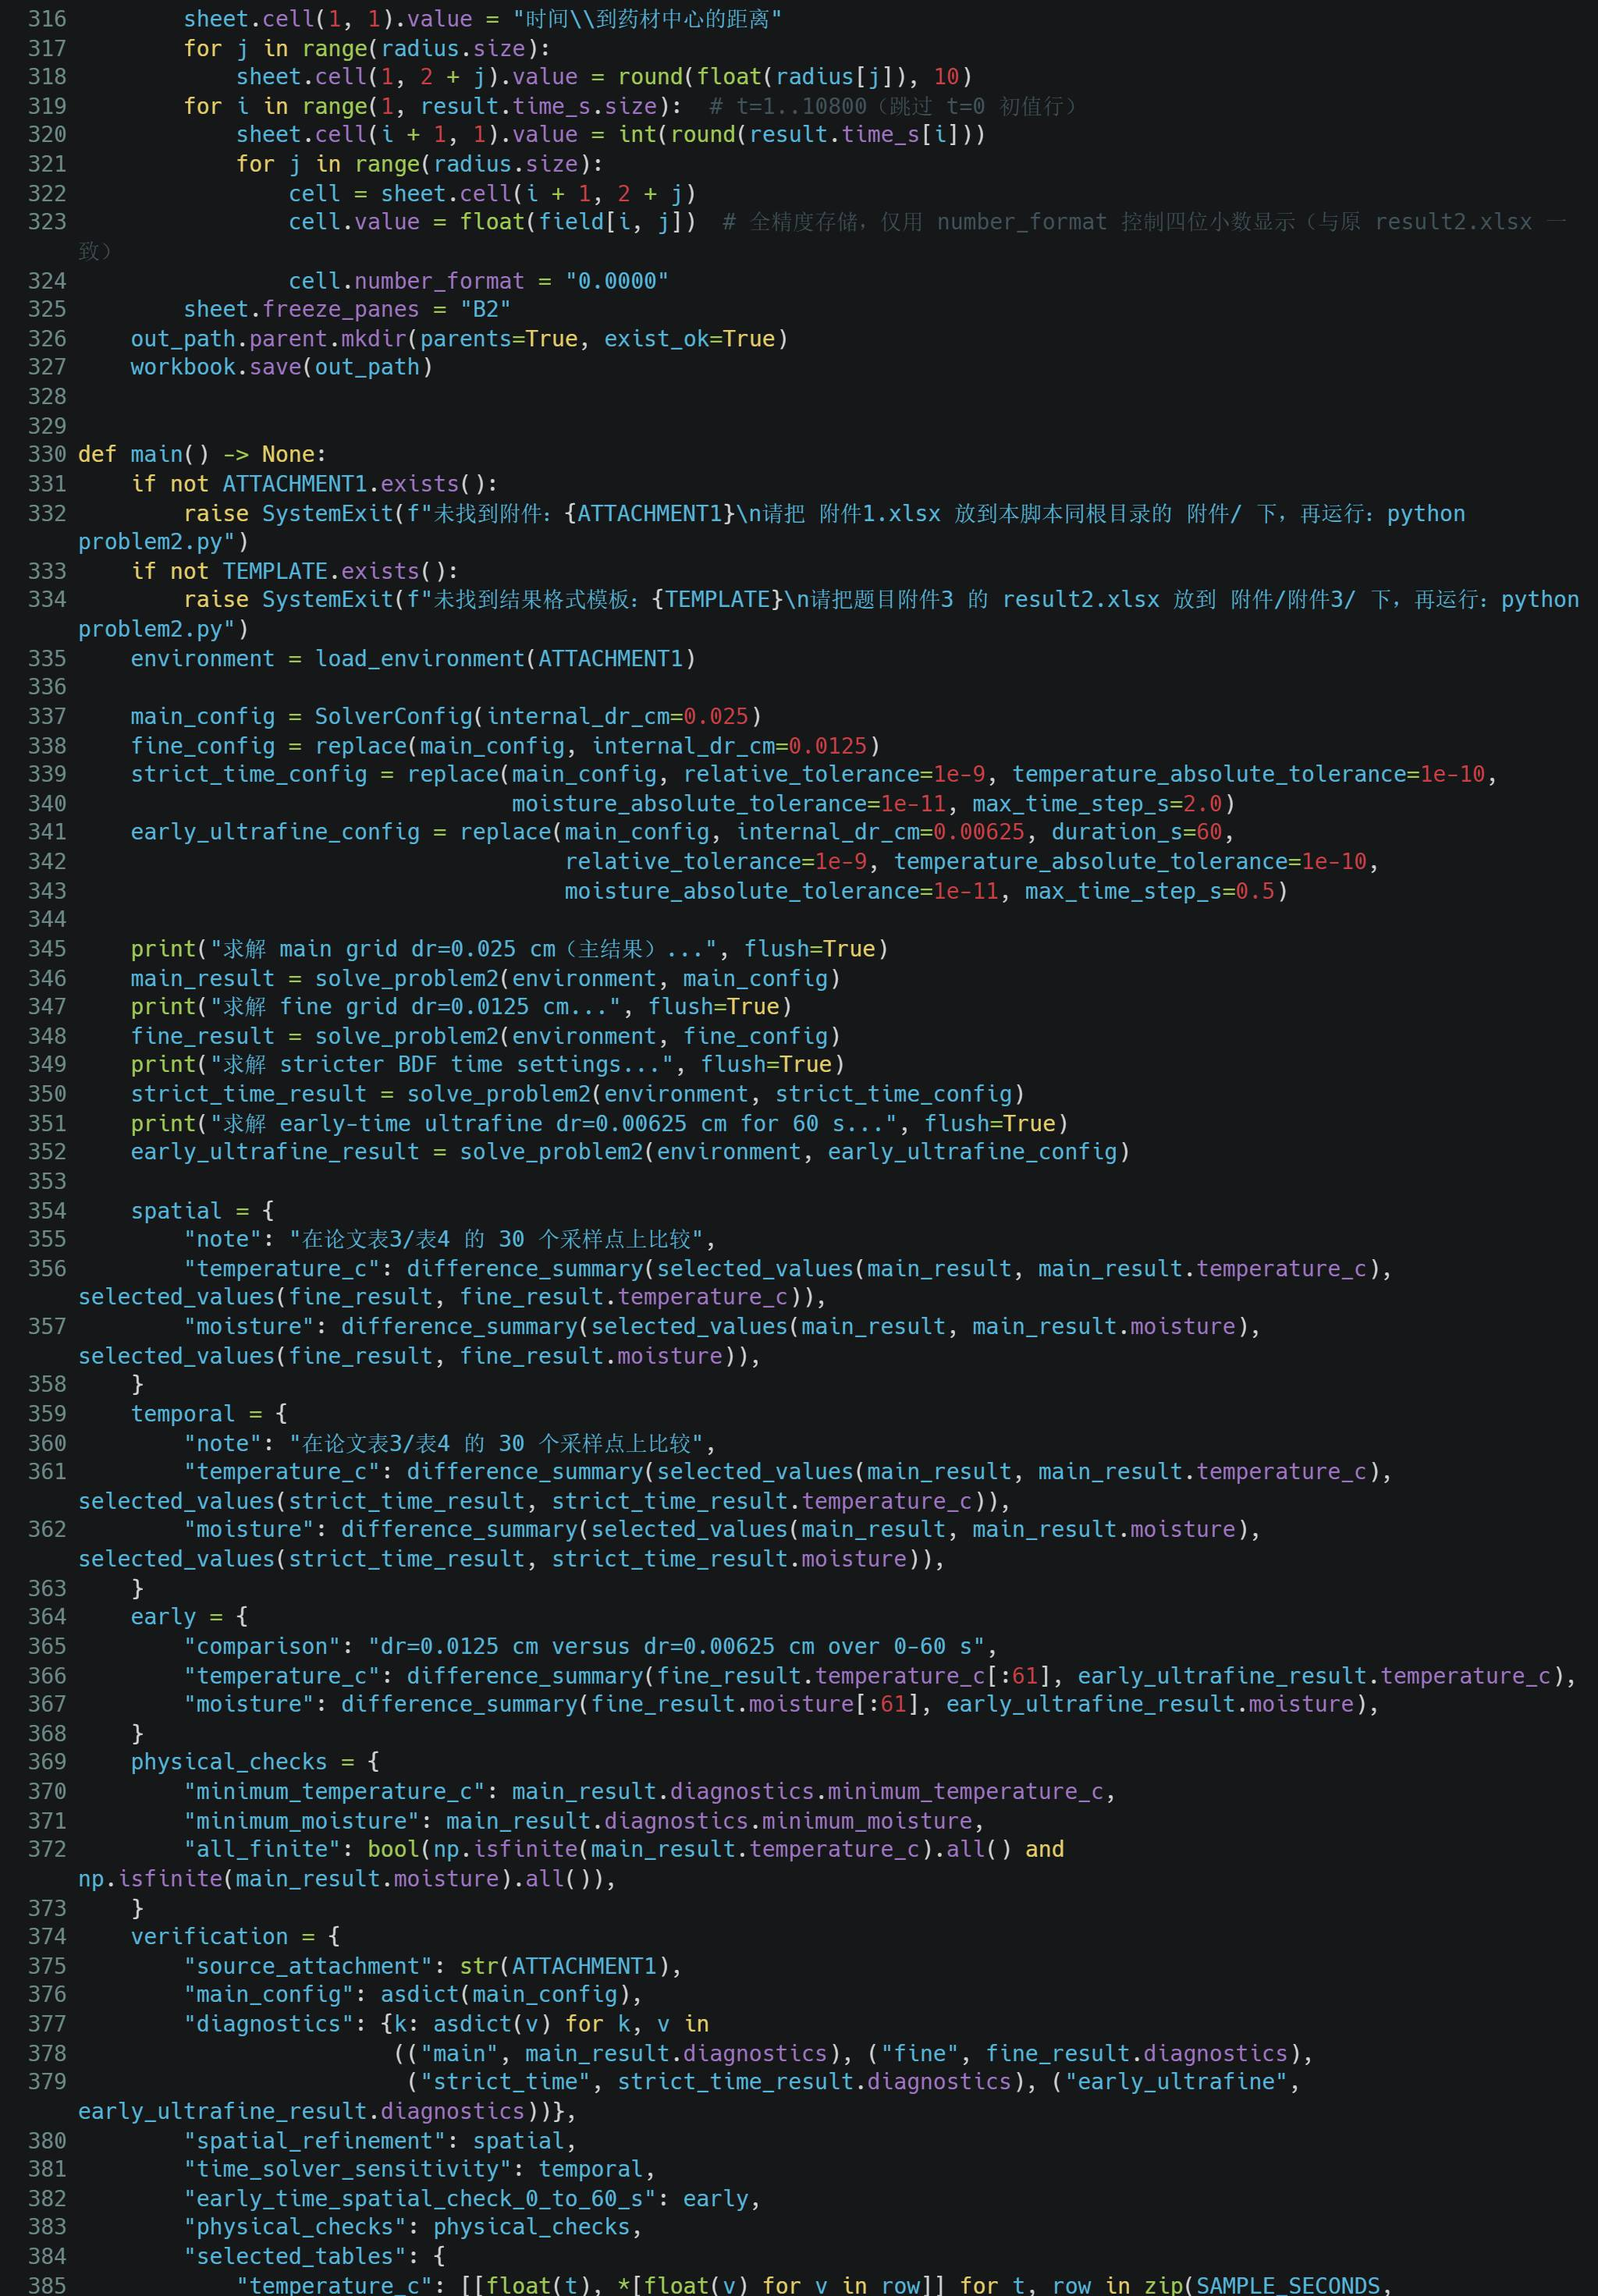
\includegraphics[width=\dimexpr\textwidth-24pt\relax]{../../code/submission/code_images/split/problem2_p5.jpg}
\newpage
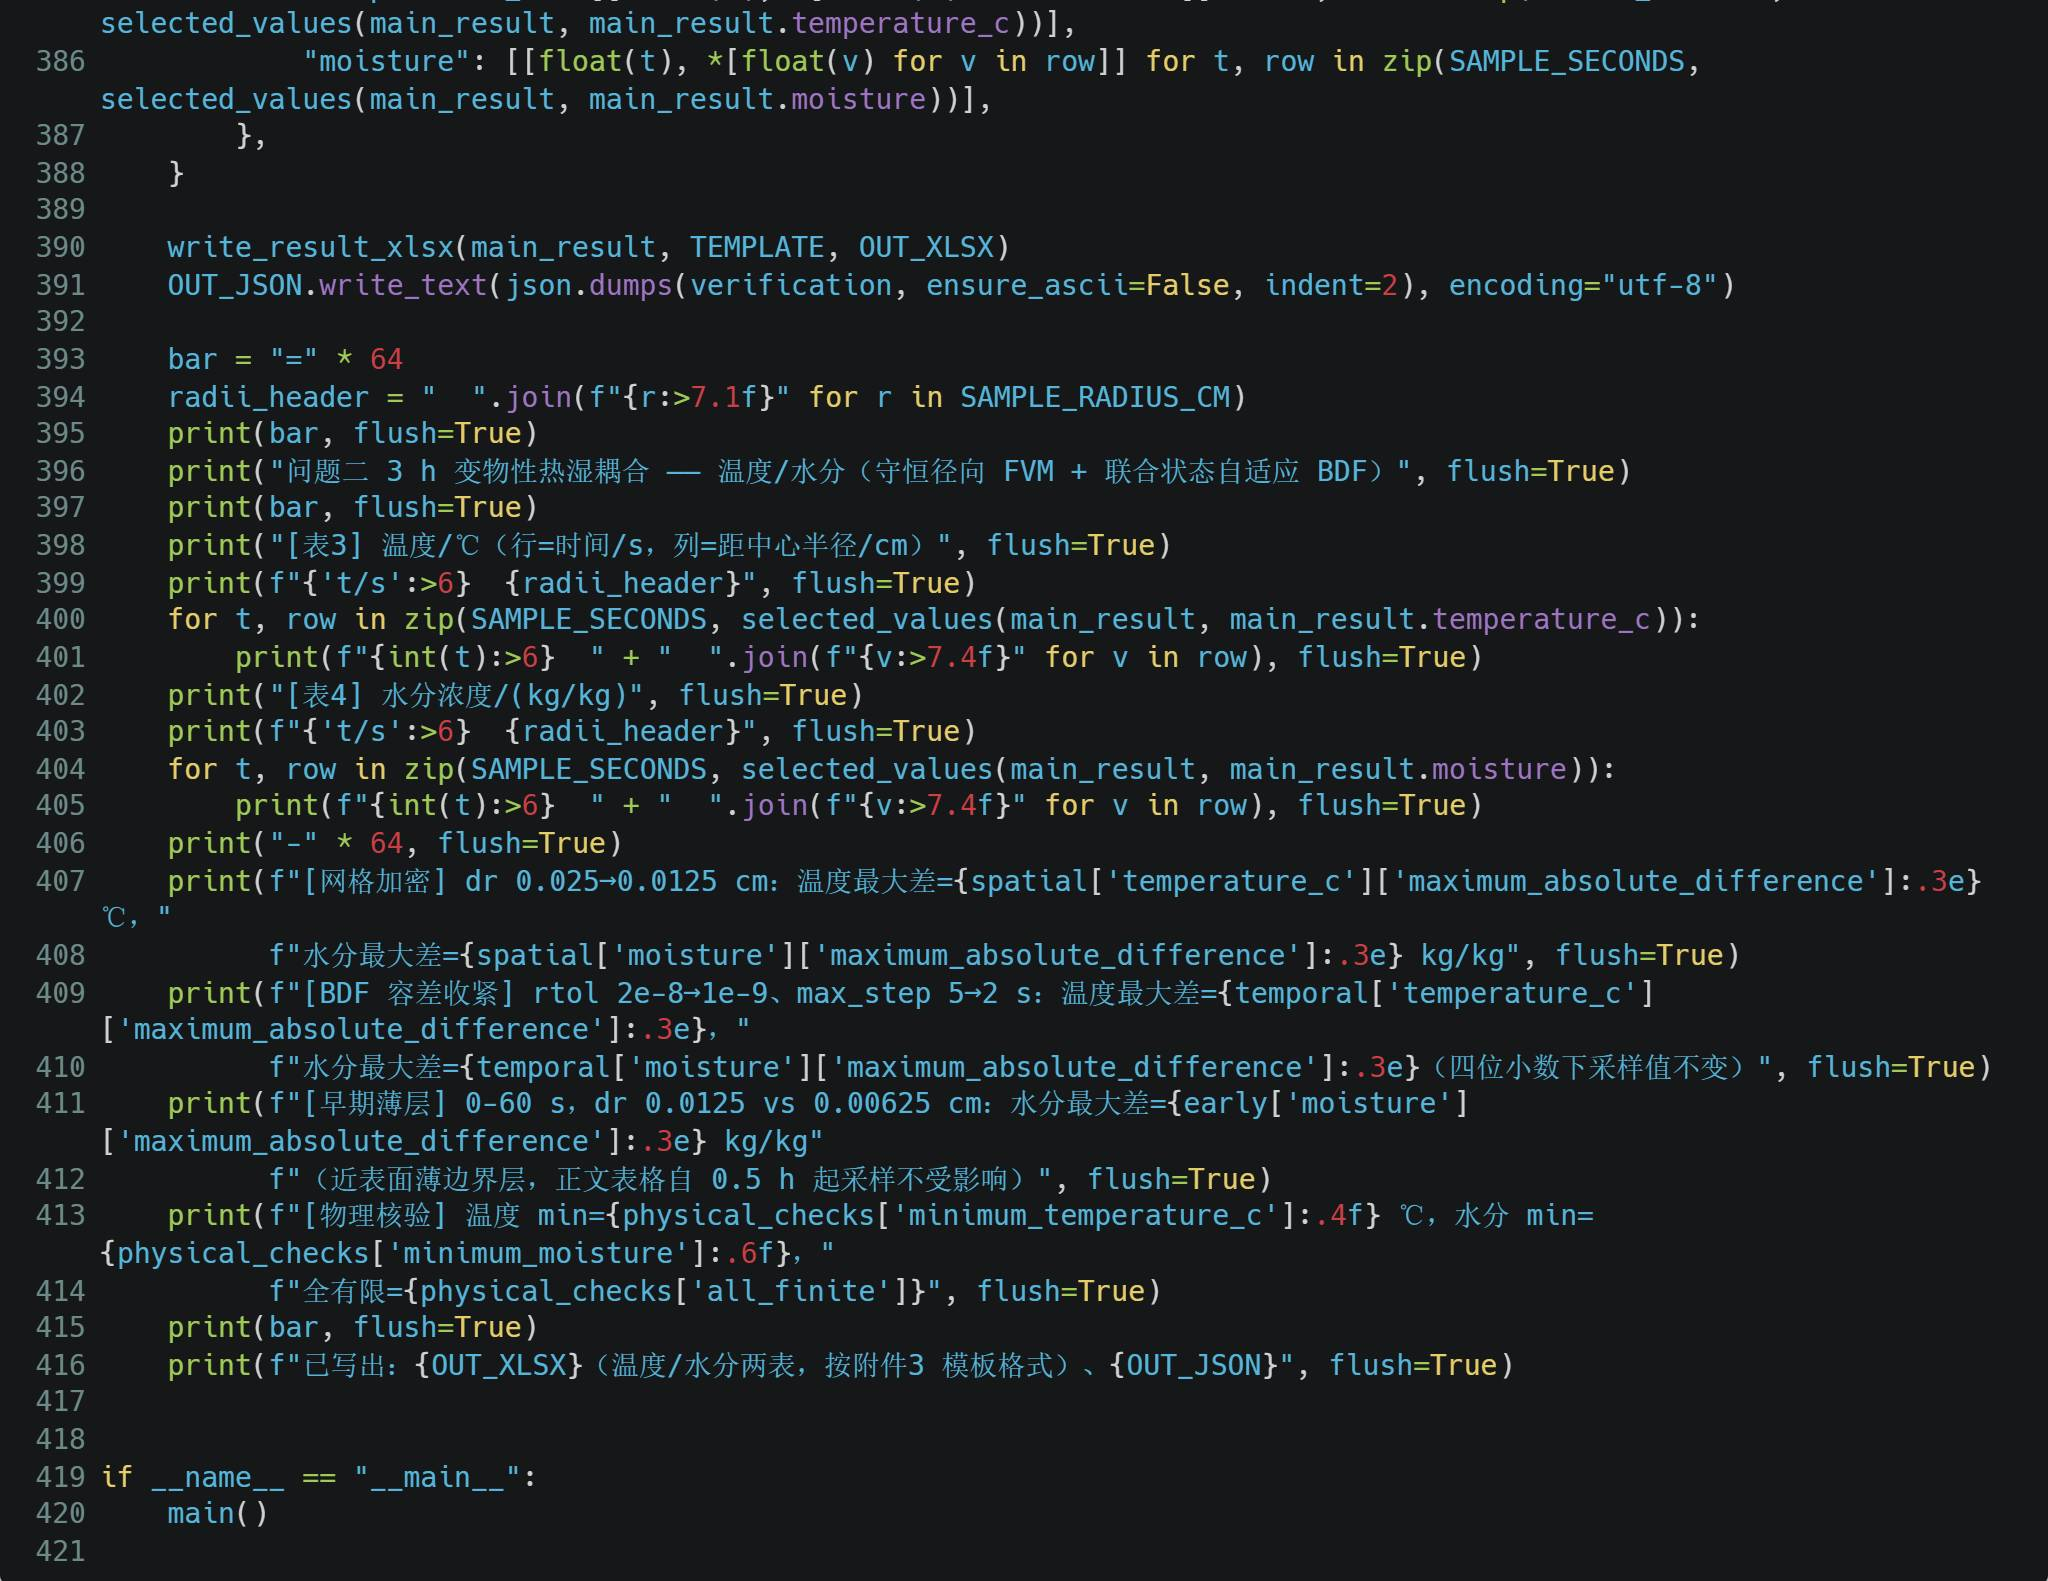
\includegraphics[width=\dimexpr\textwidth-24pt\relax]{../../code/submission/code_images/split/problem2_p6.jpg}
\newpage
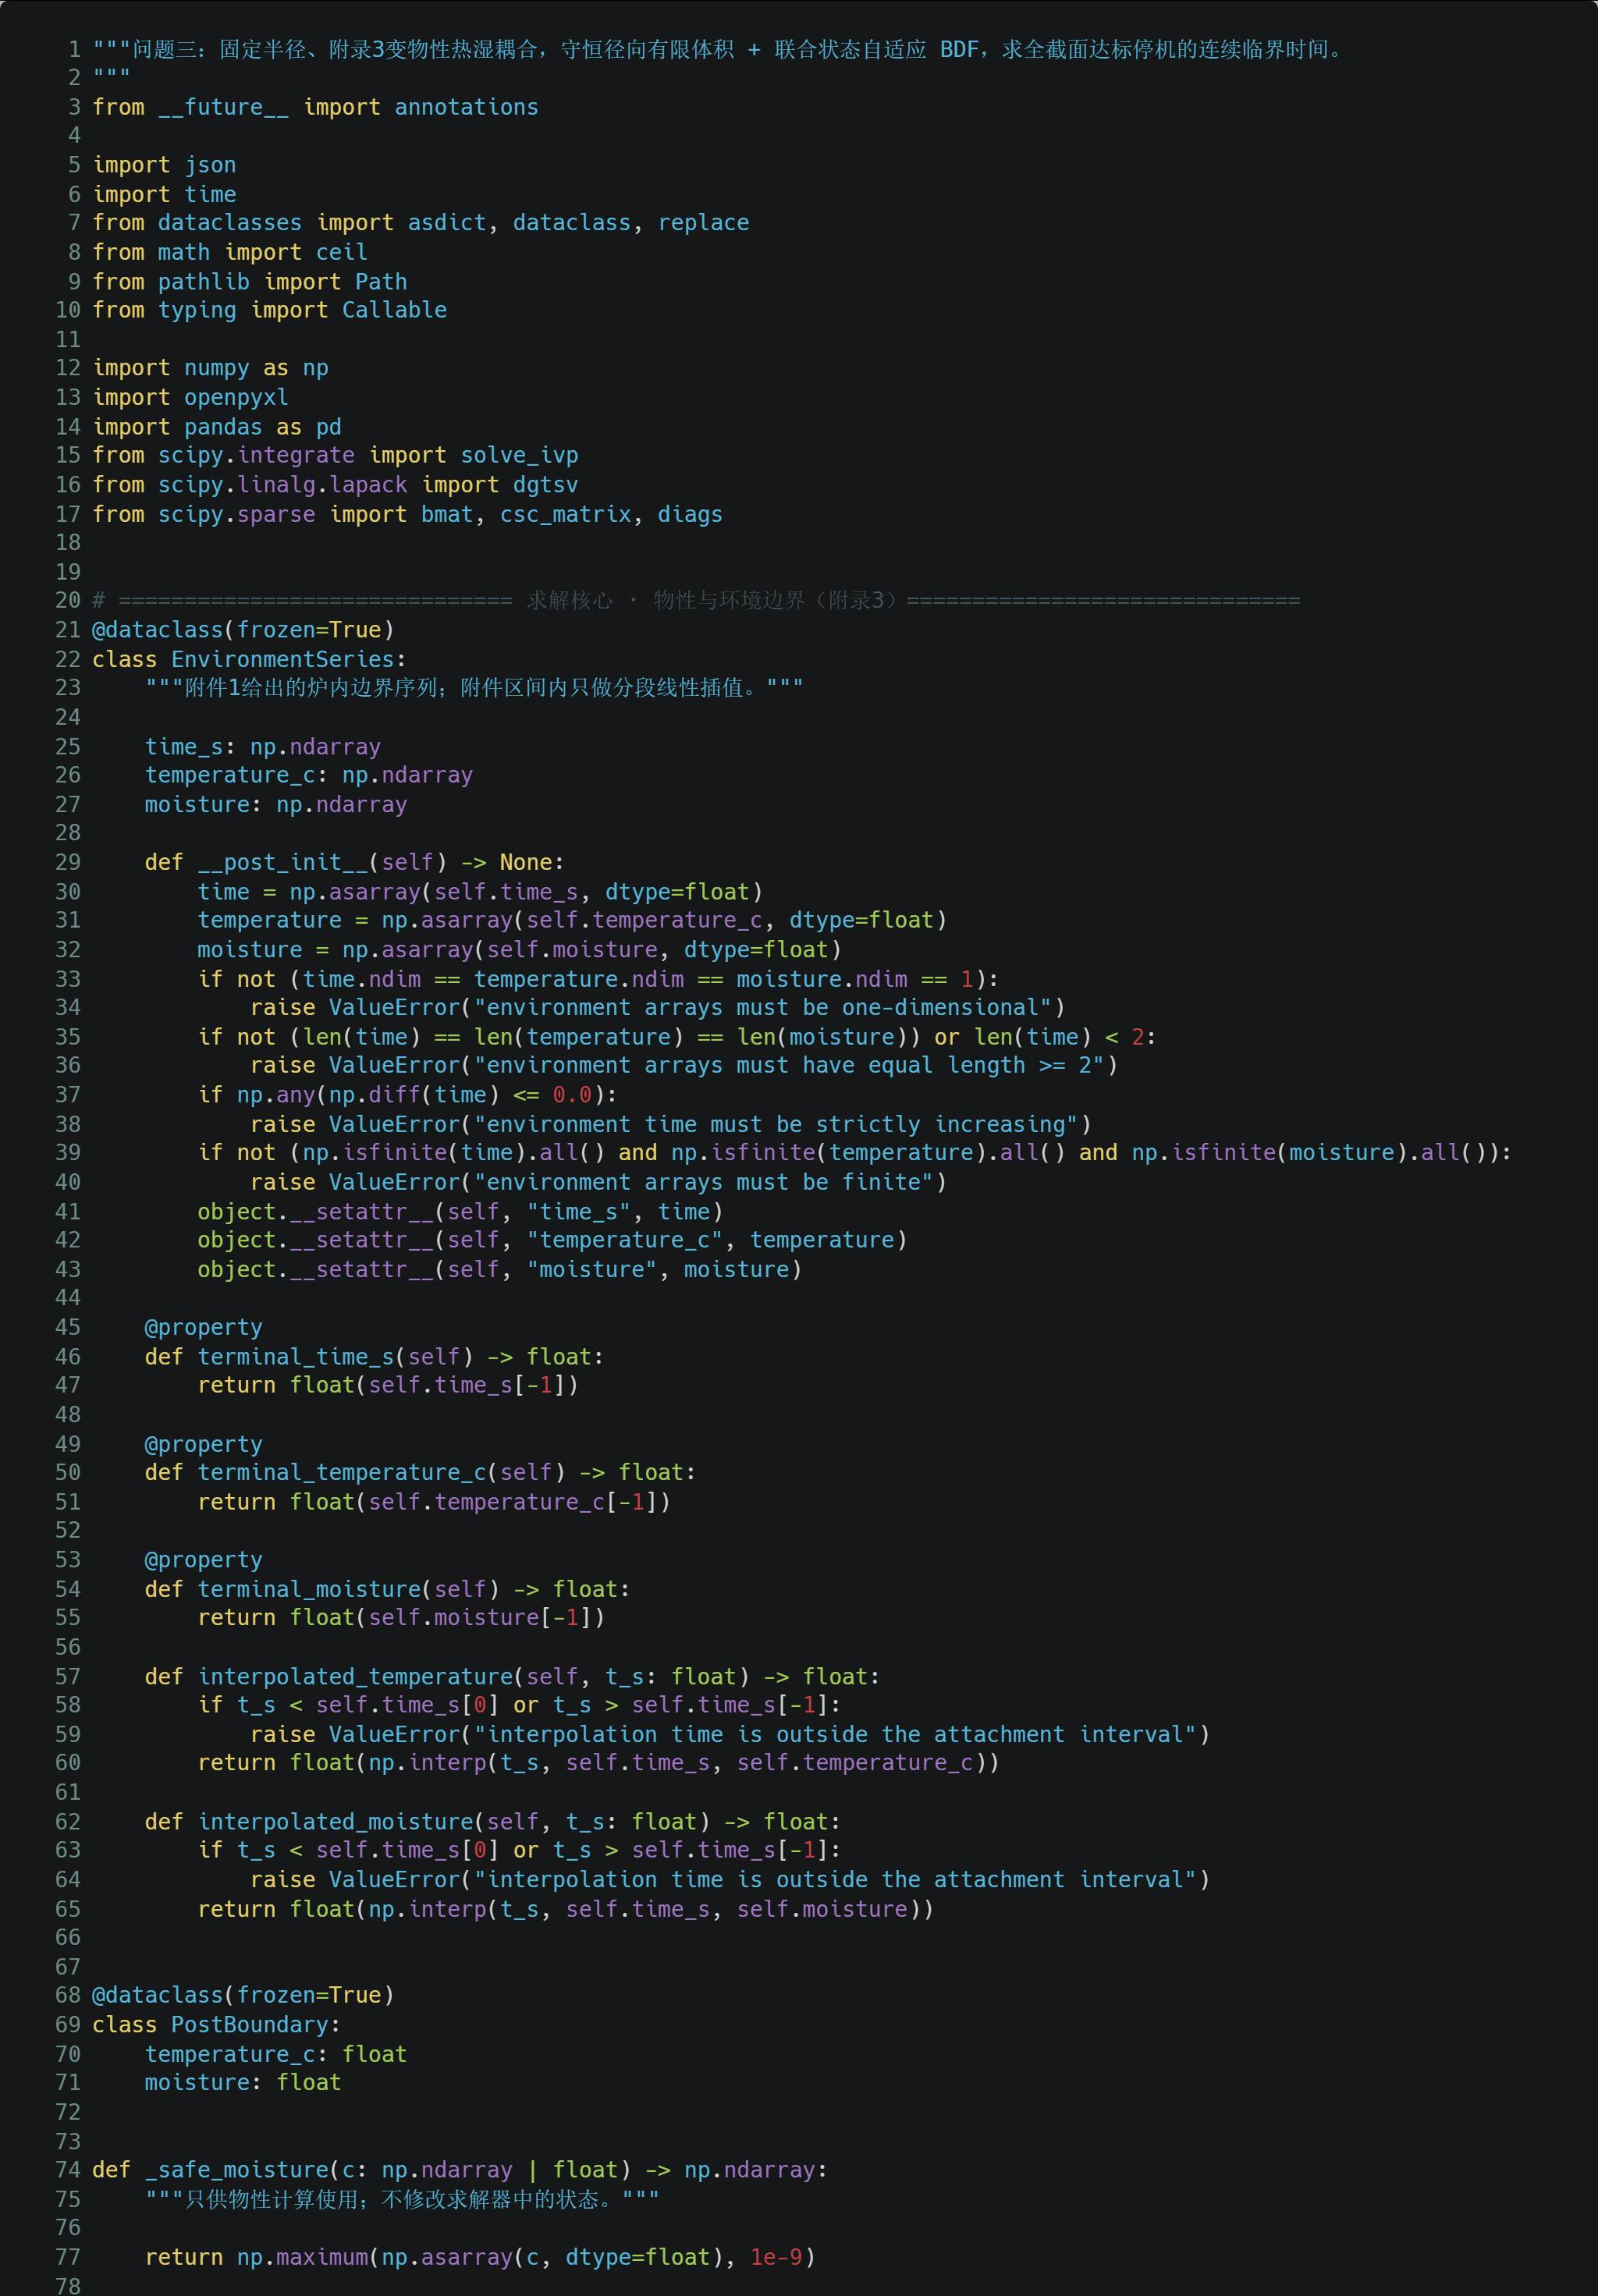
\includegraphics[width=\dimexpr\textwidth-24pt\relax]{../../code/submission/code_images/split/problem3_p1.jpg}
\newpage
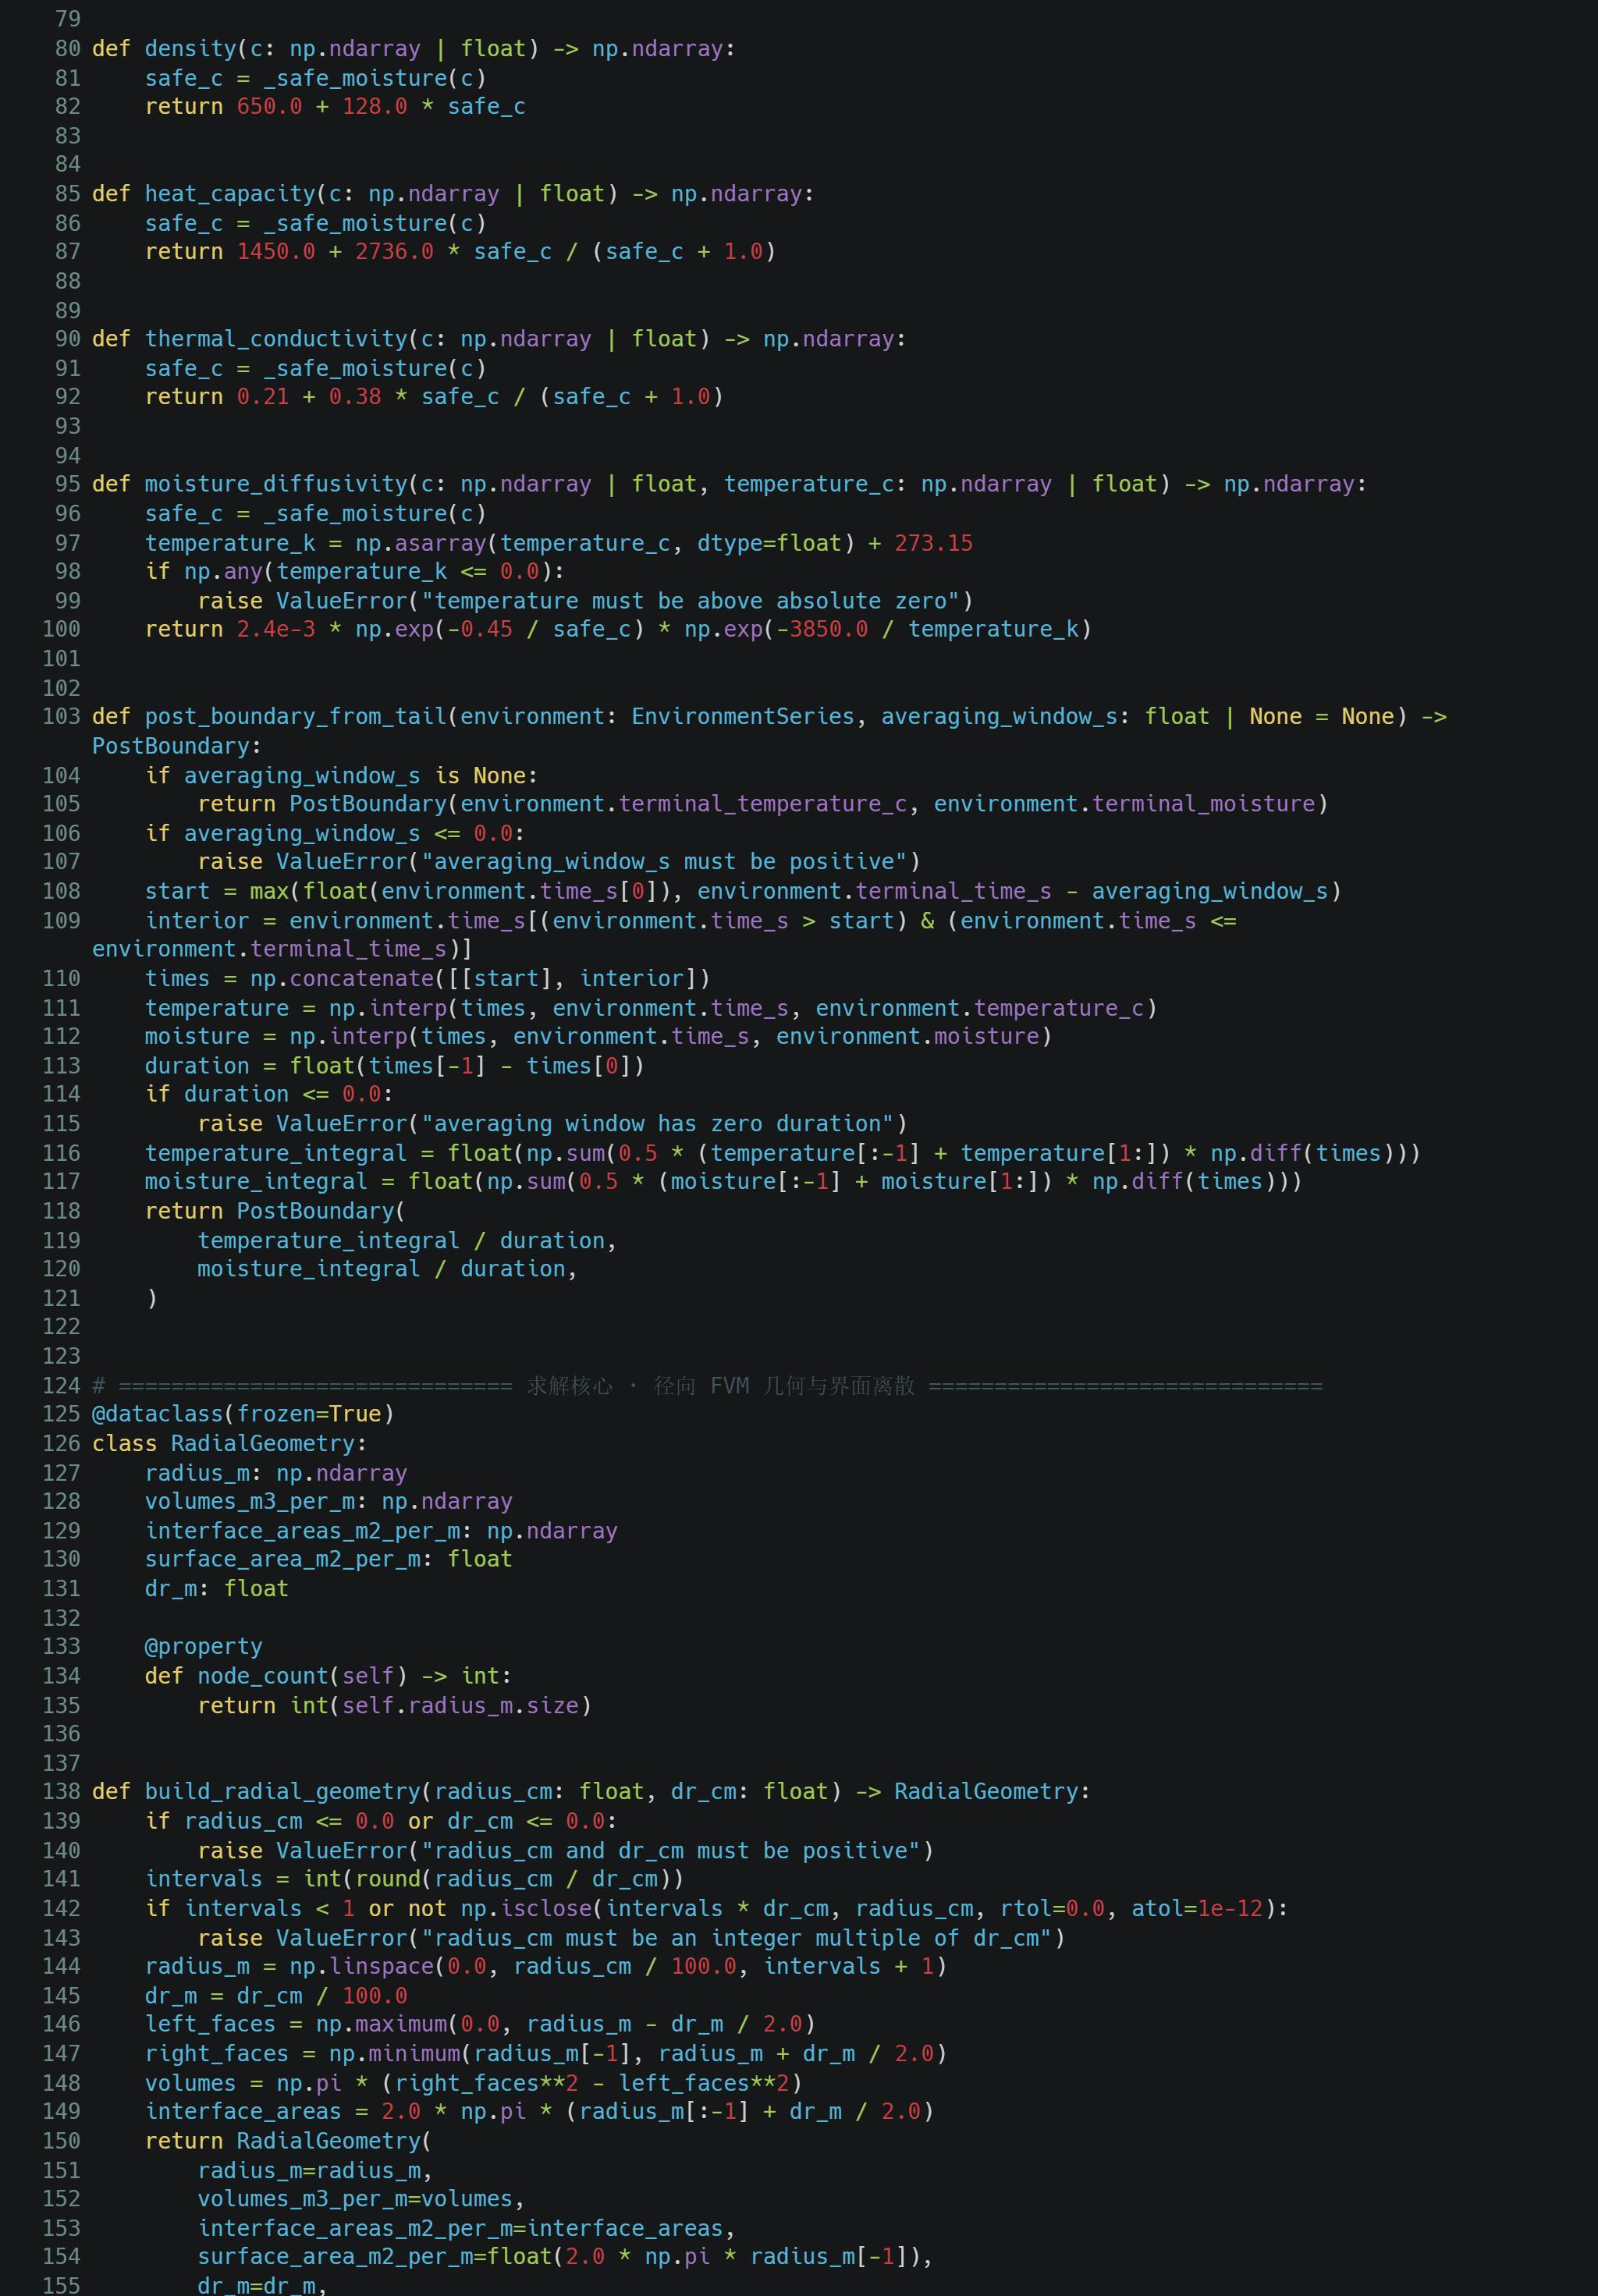
\includegraphics[width=\dimexpr\textwidth-24pt\relax]{../../code/submission/code_images/split/problem3_p2.jpg}
\newpage
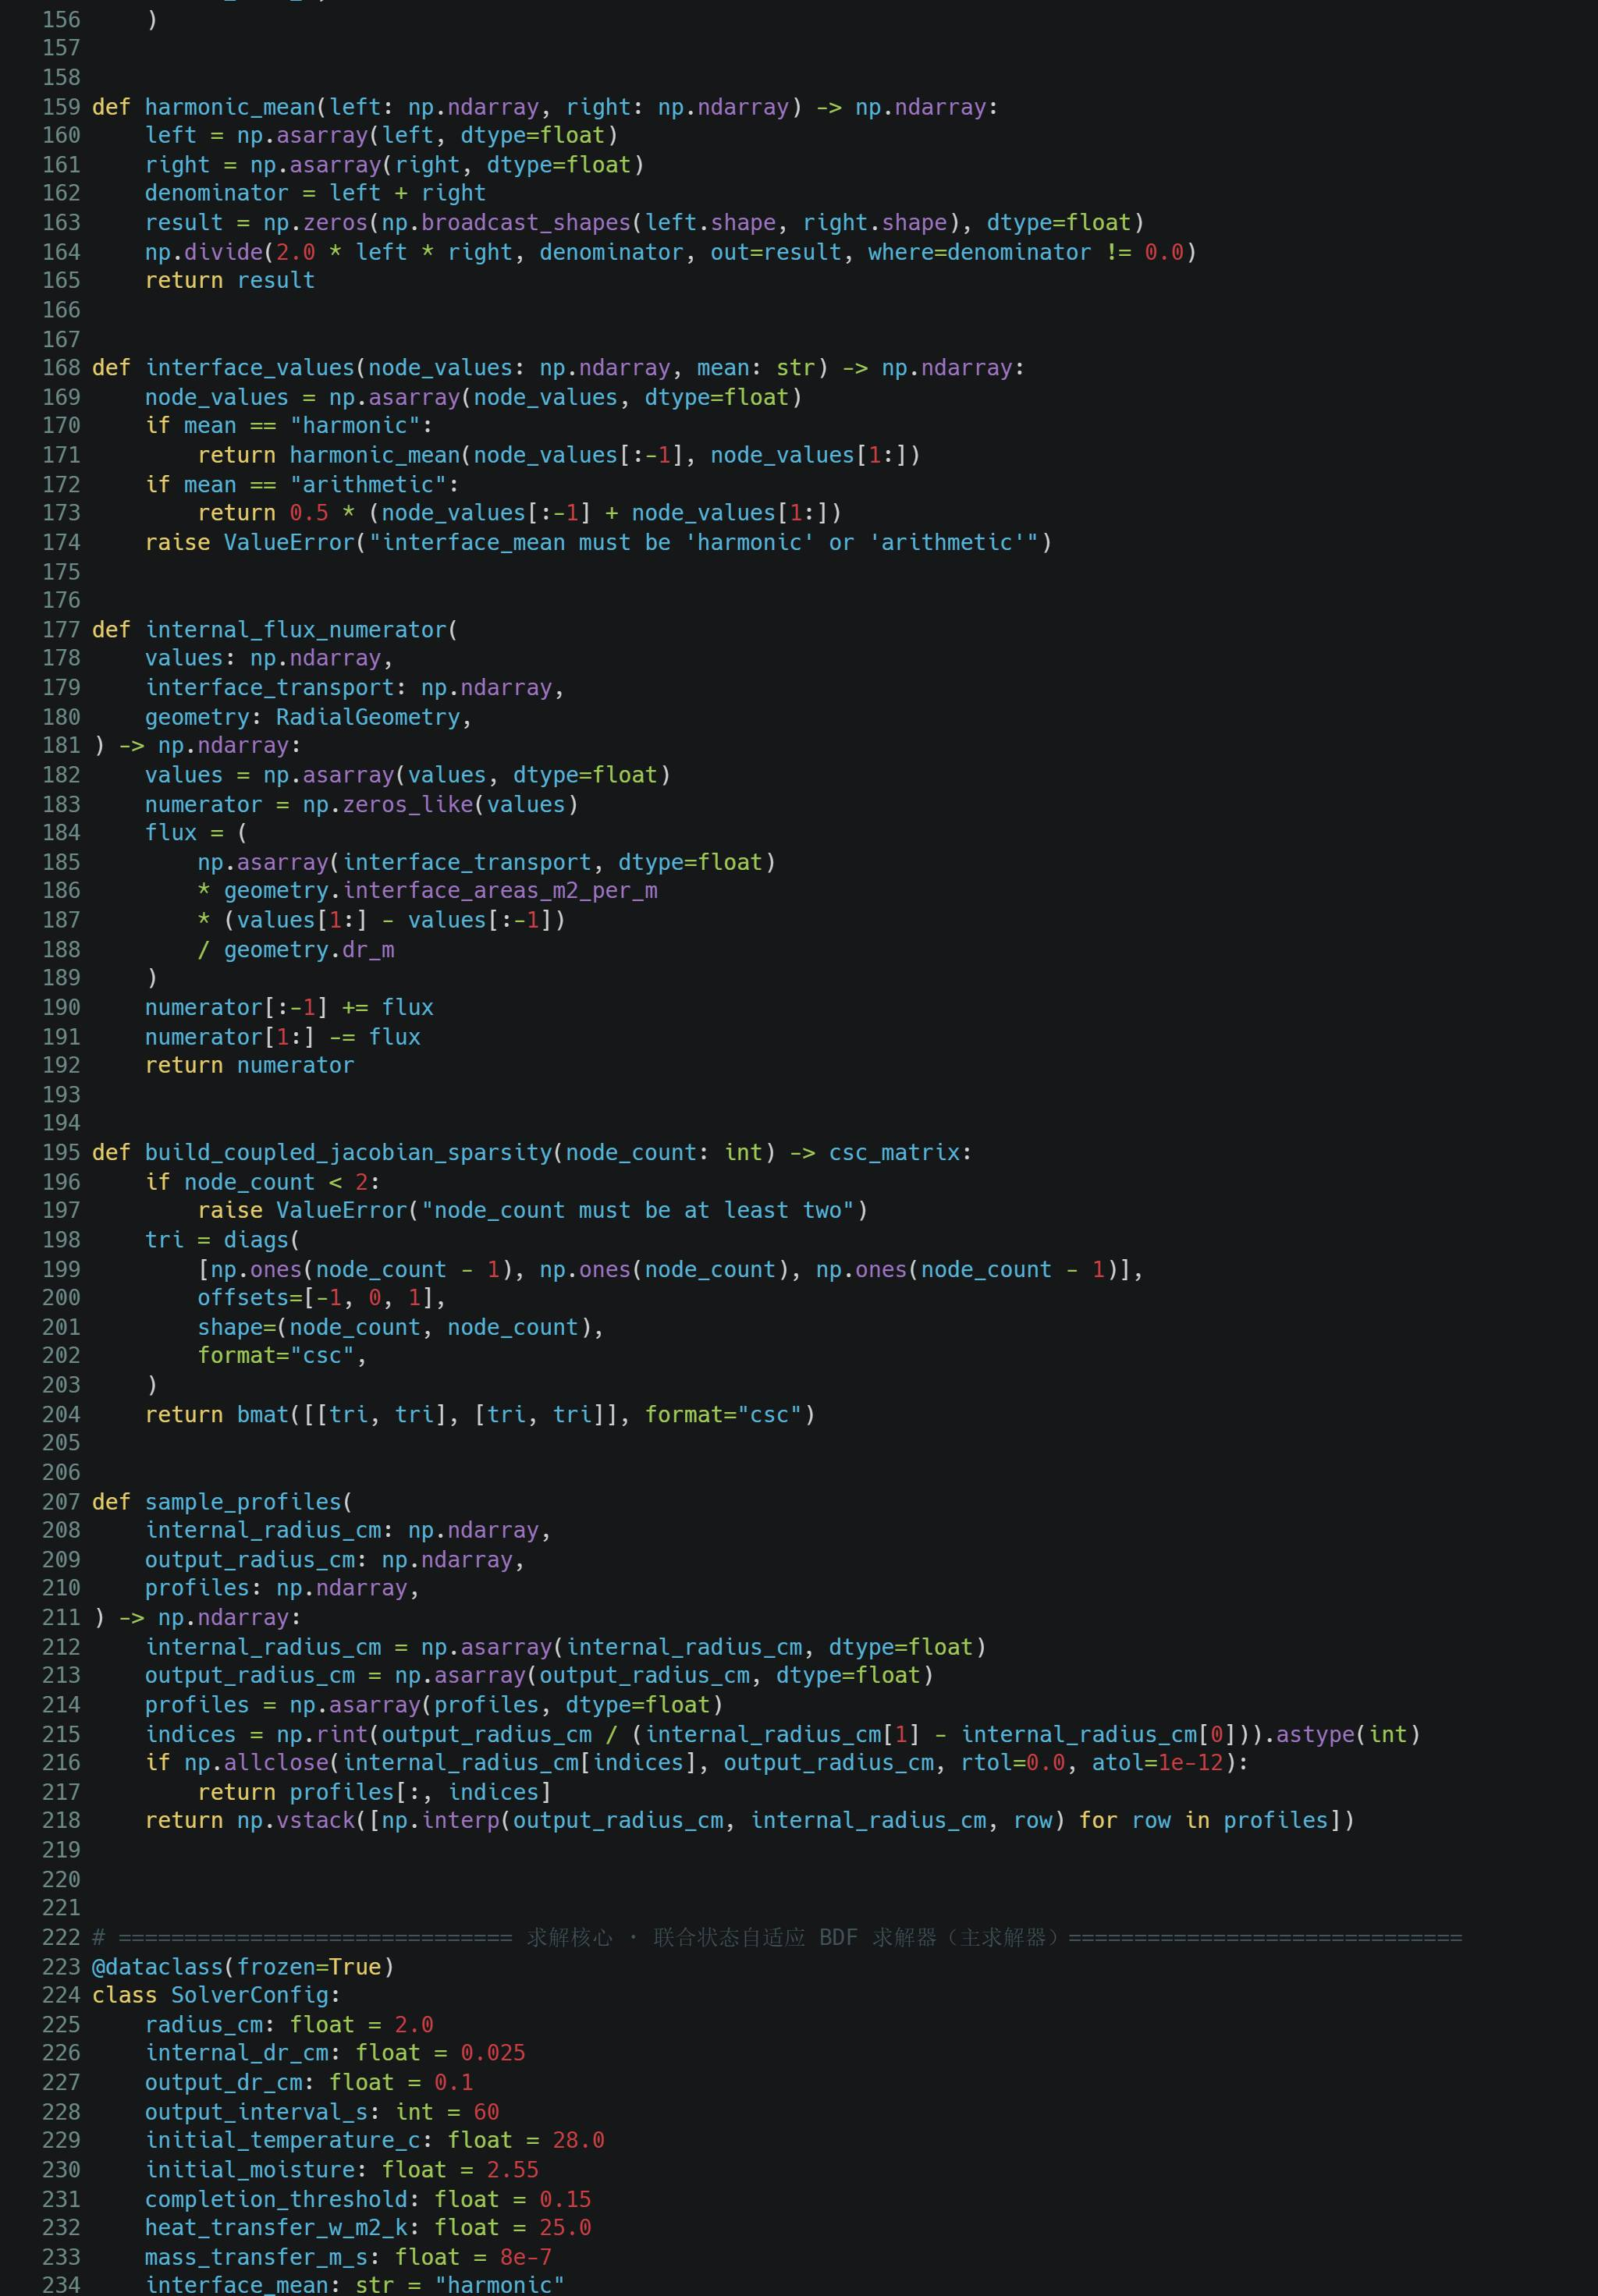
\includegraphics[width=\dimexpr\textwidth-24pt\relax]{../../code/submission/code_images/split/problem3_p3.jpg}
\newpage
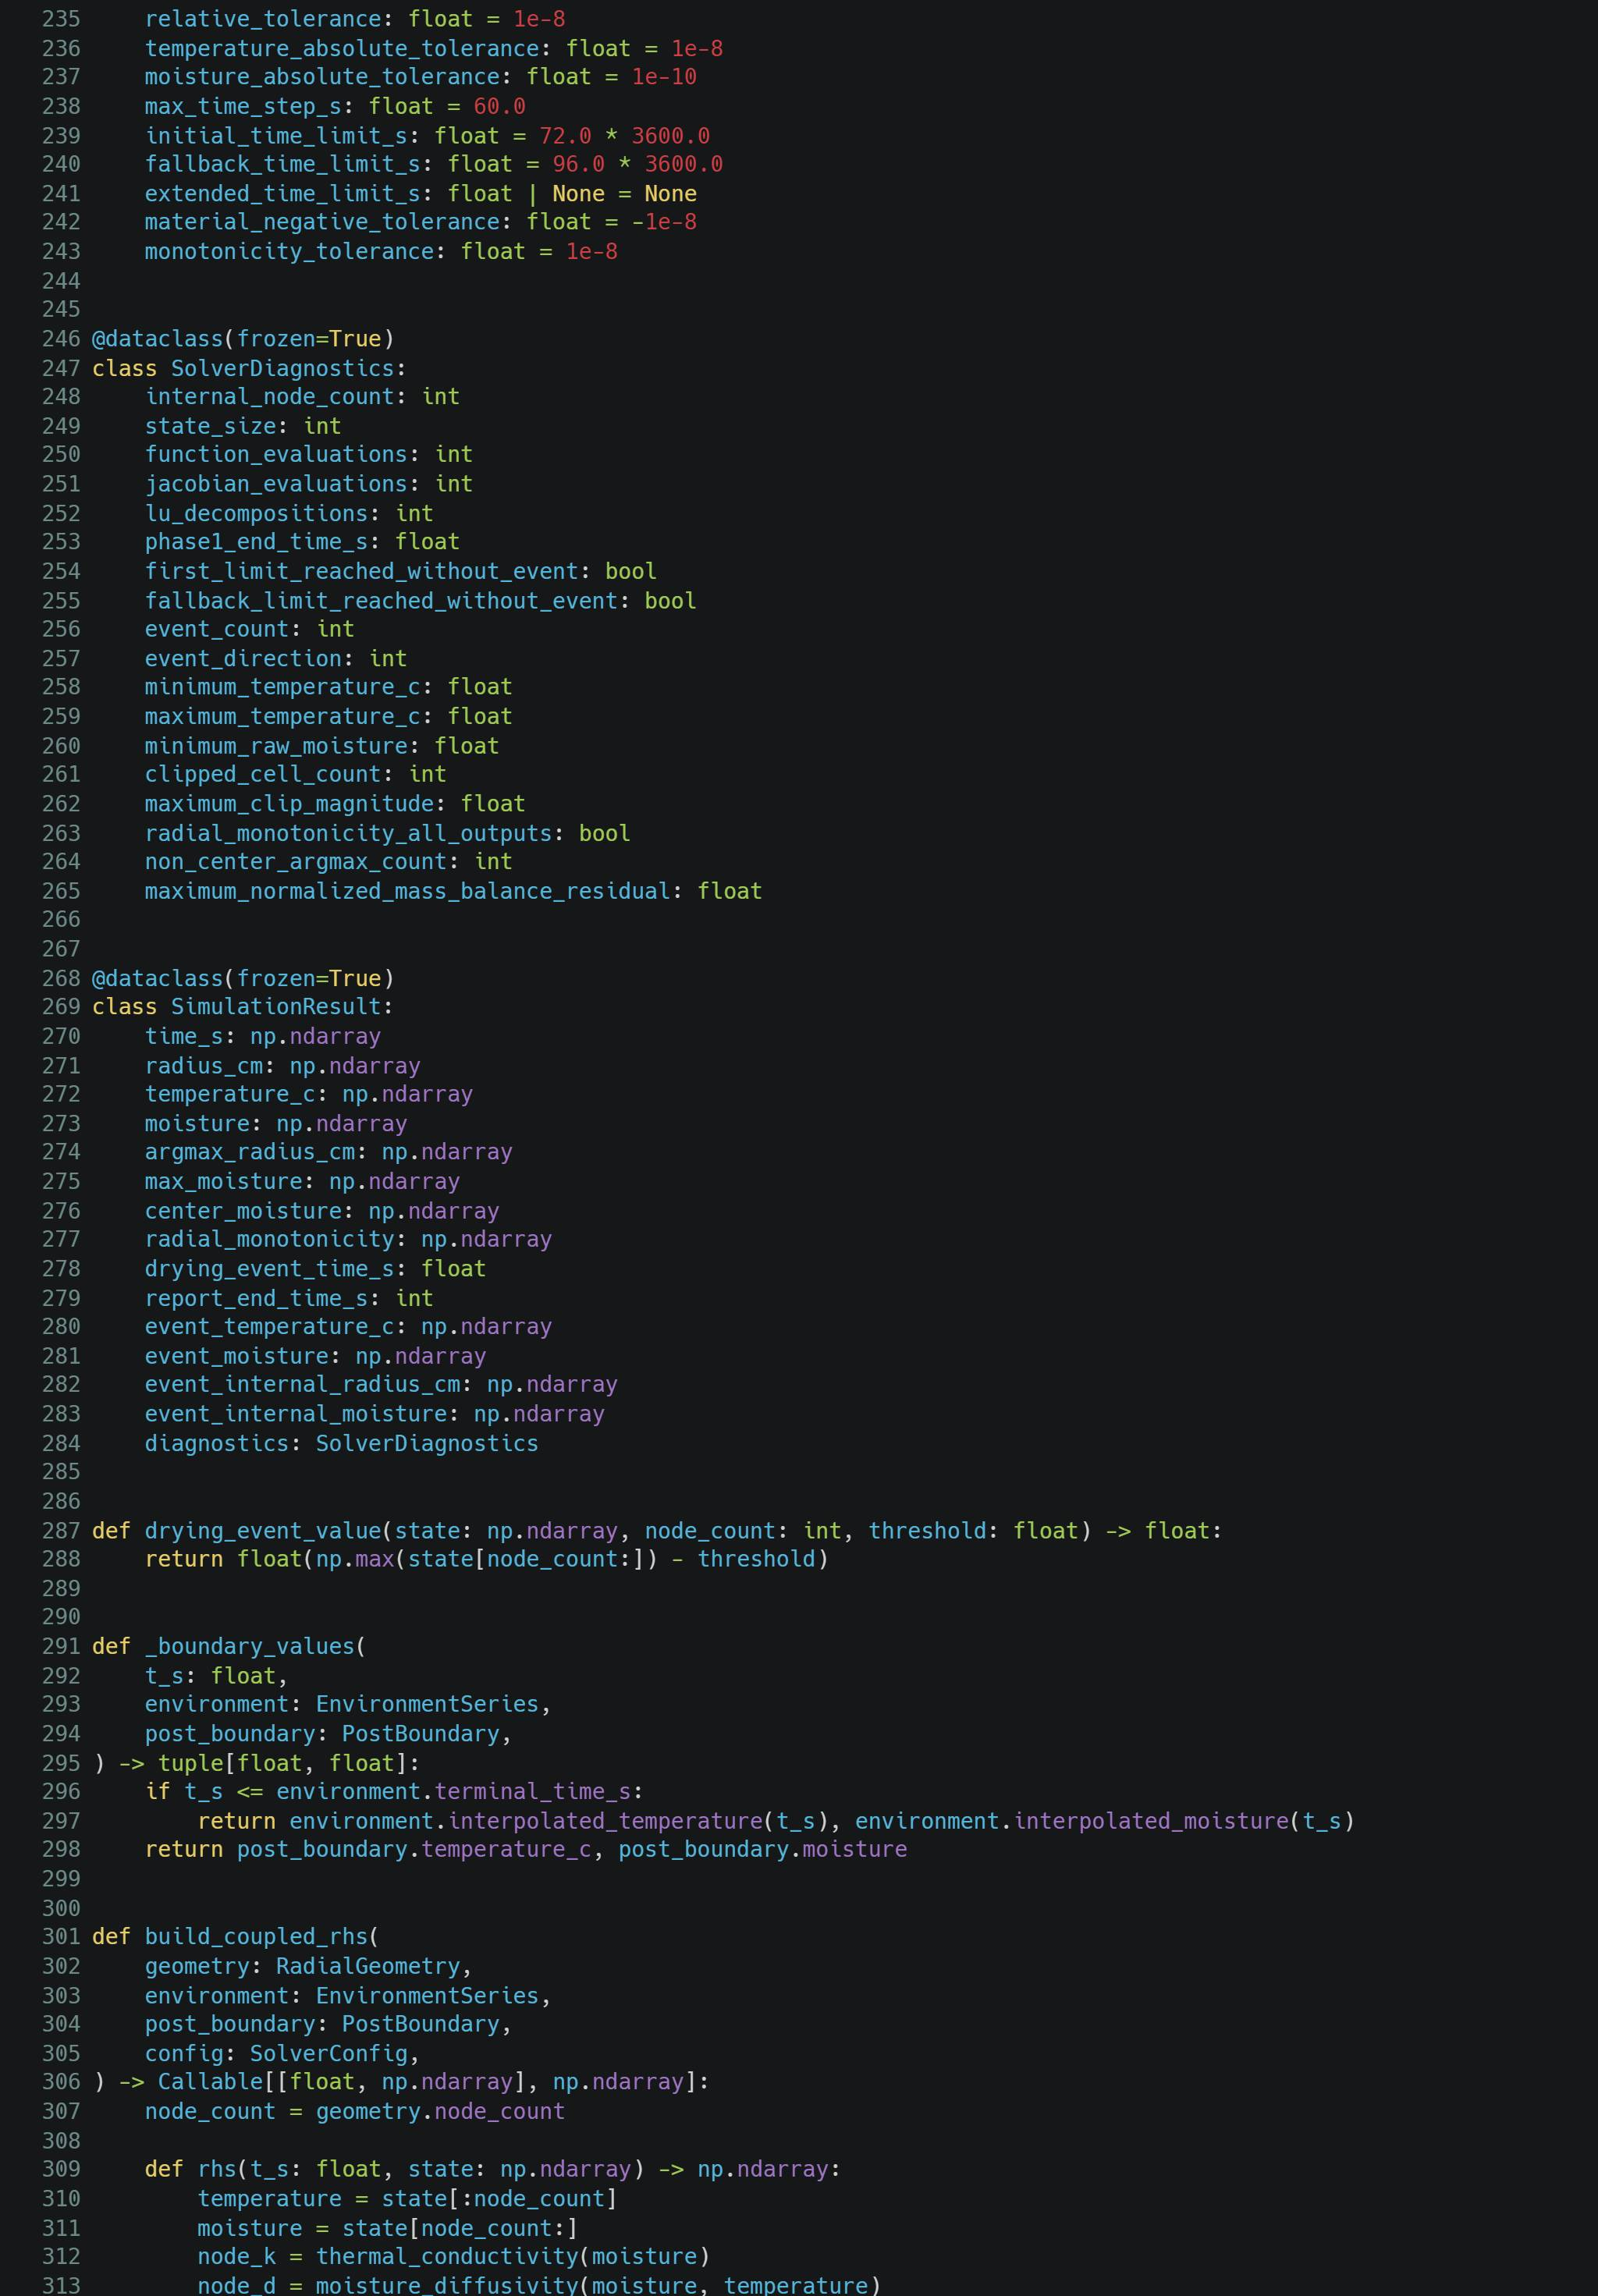
\includegraphics[width=\dimexpr\textwidth-24pt\relax]{../../code/submission/code_images/split/problem3_p4.jpg}
\newpage
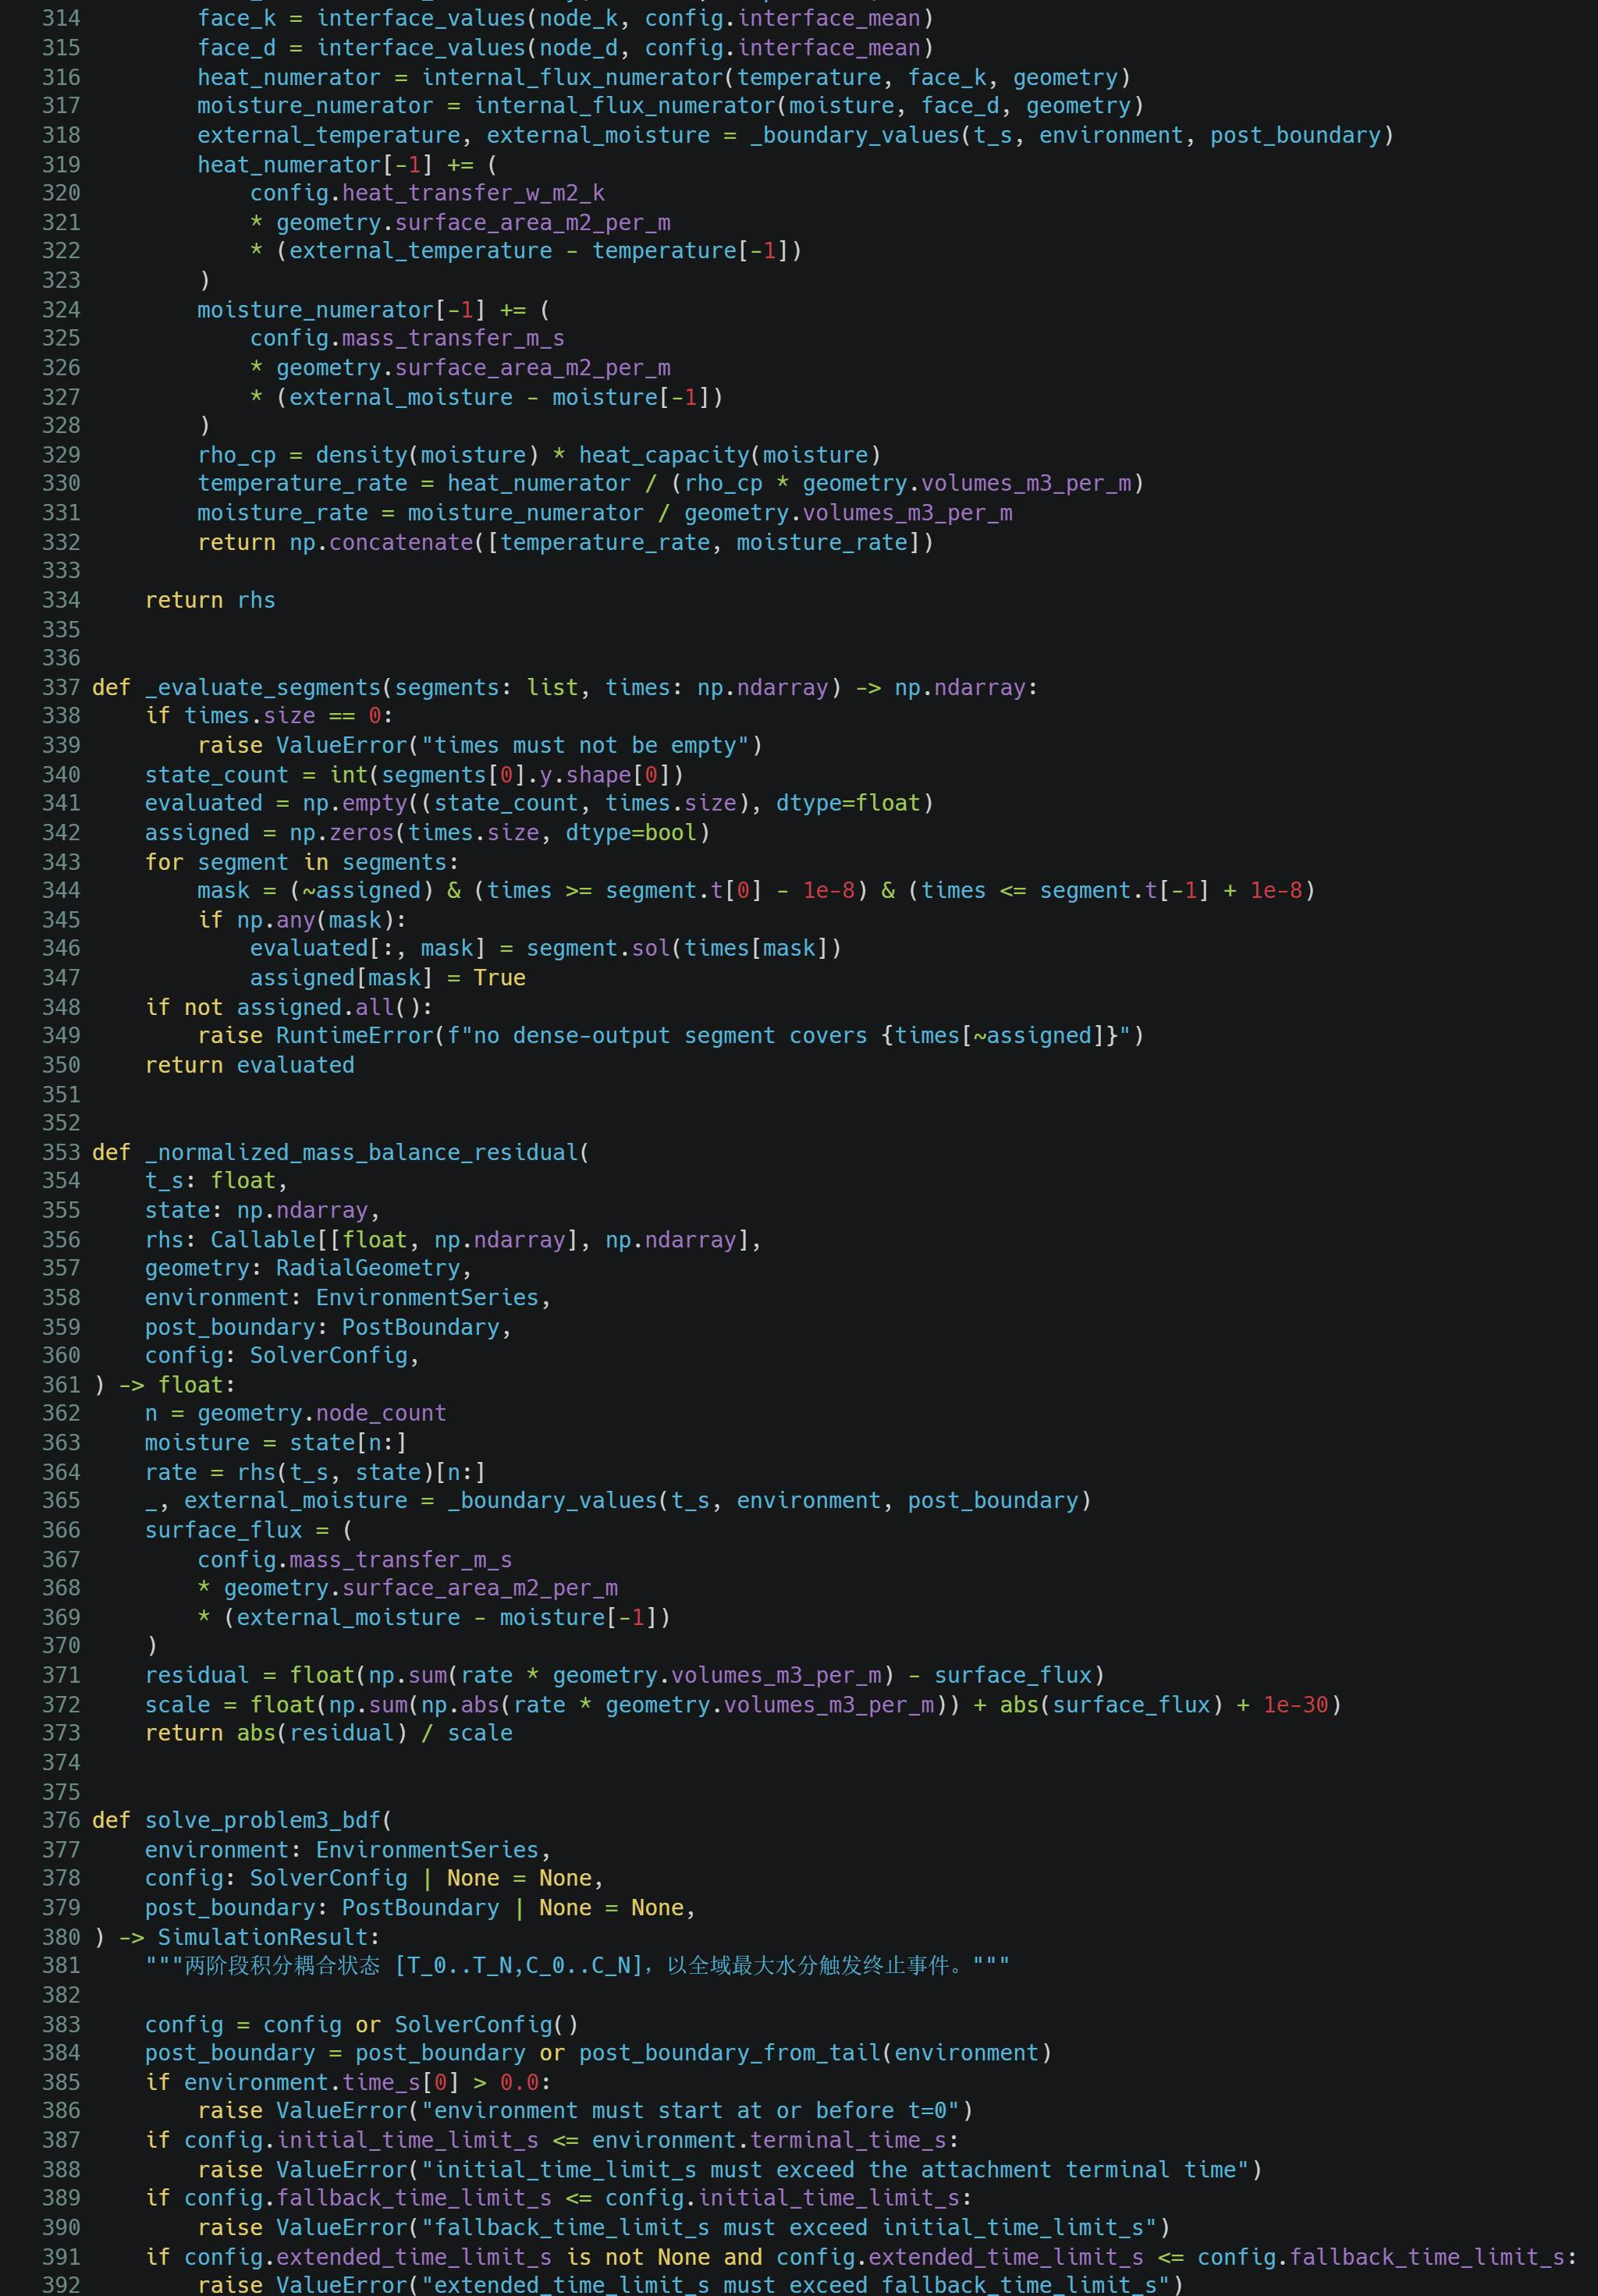
\includegraphics[width=\dimexpr\textwidth-24pt\relax]{../../code/submission/code_images/split/problem3_p5.jpg}
\newpage
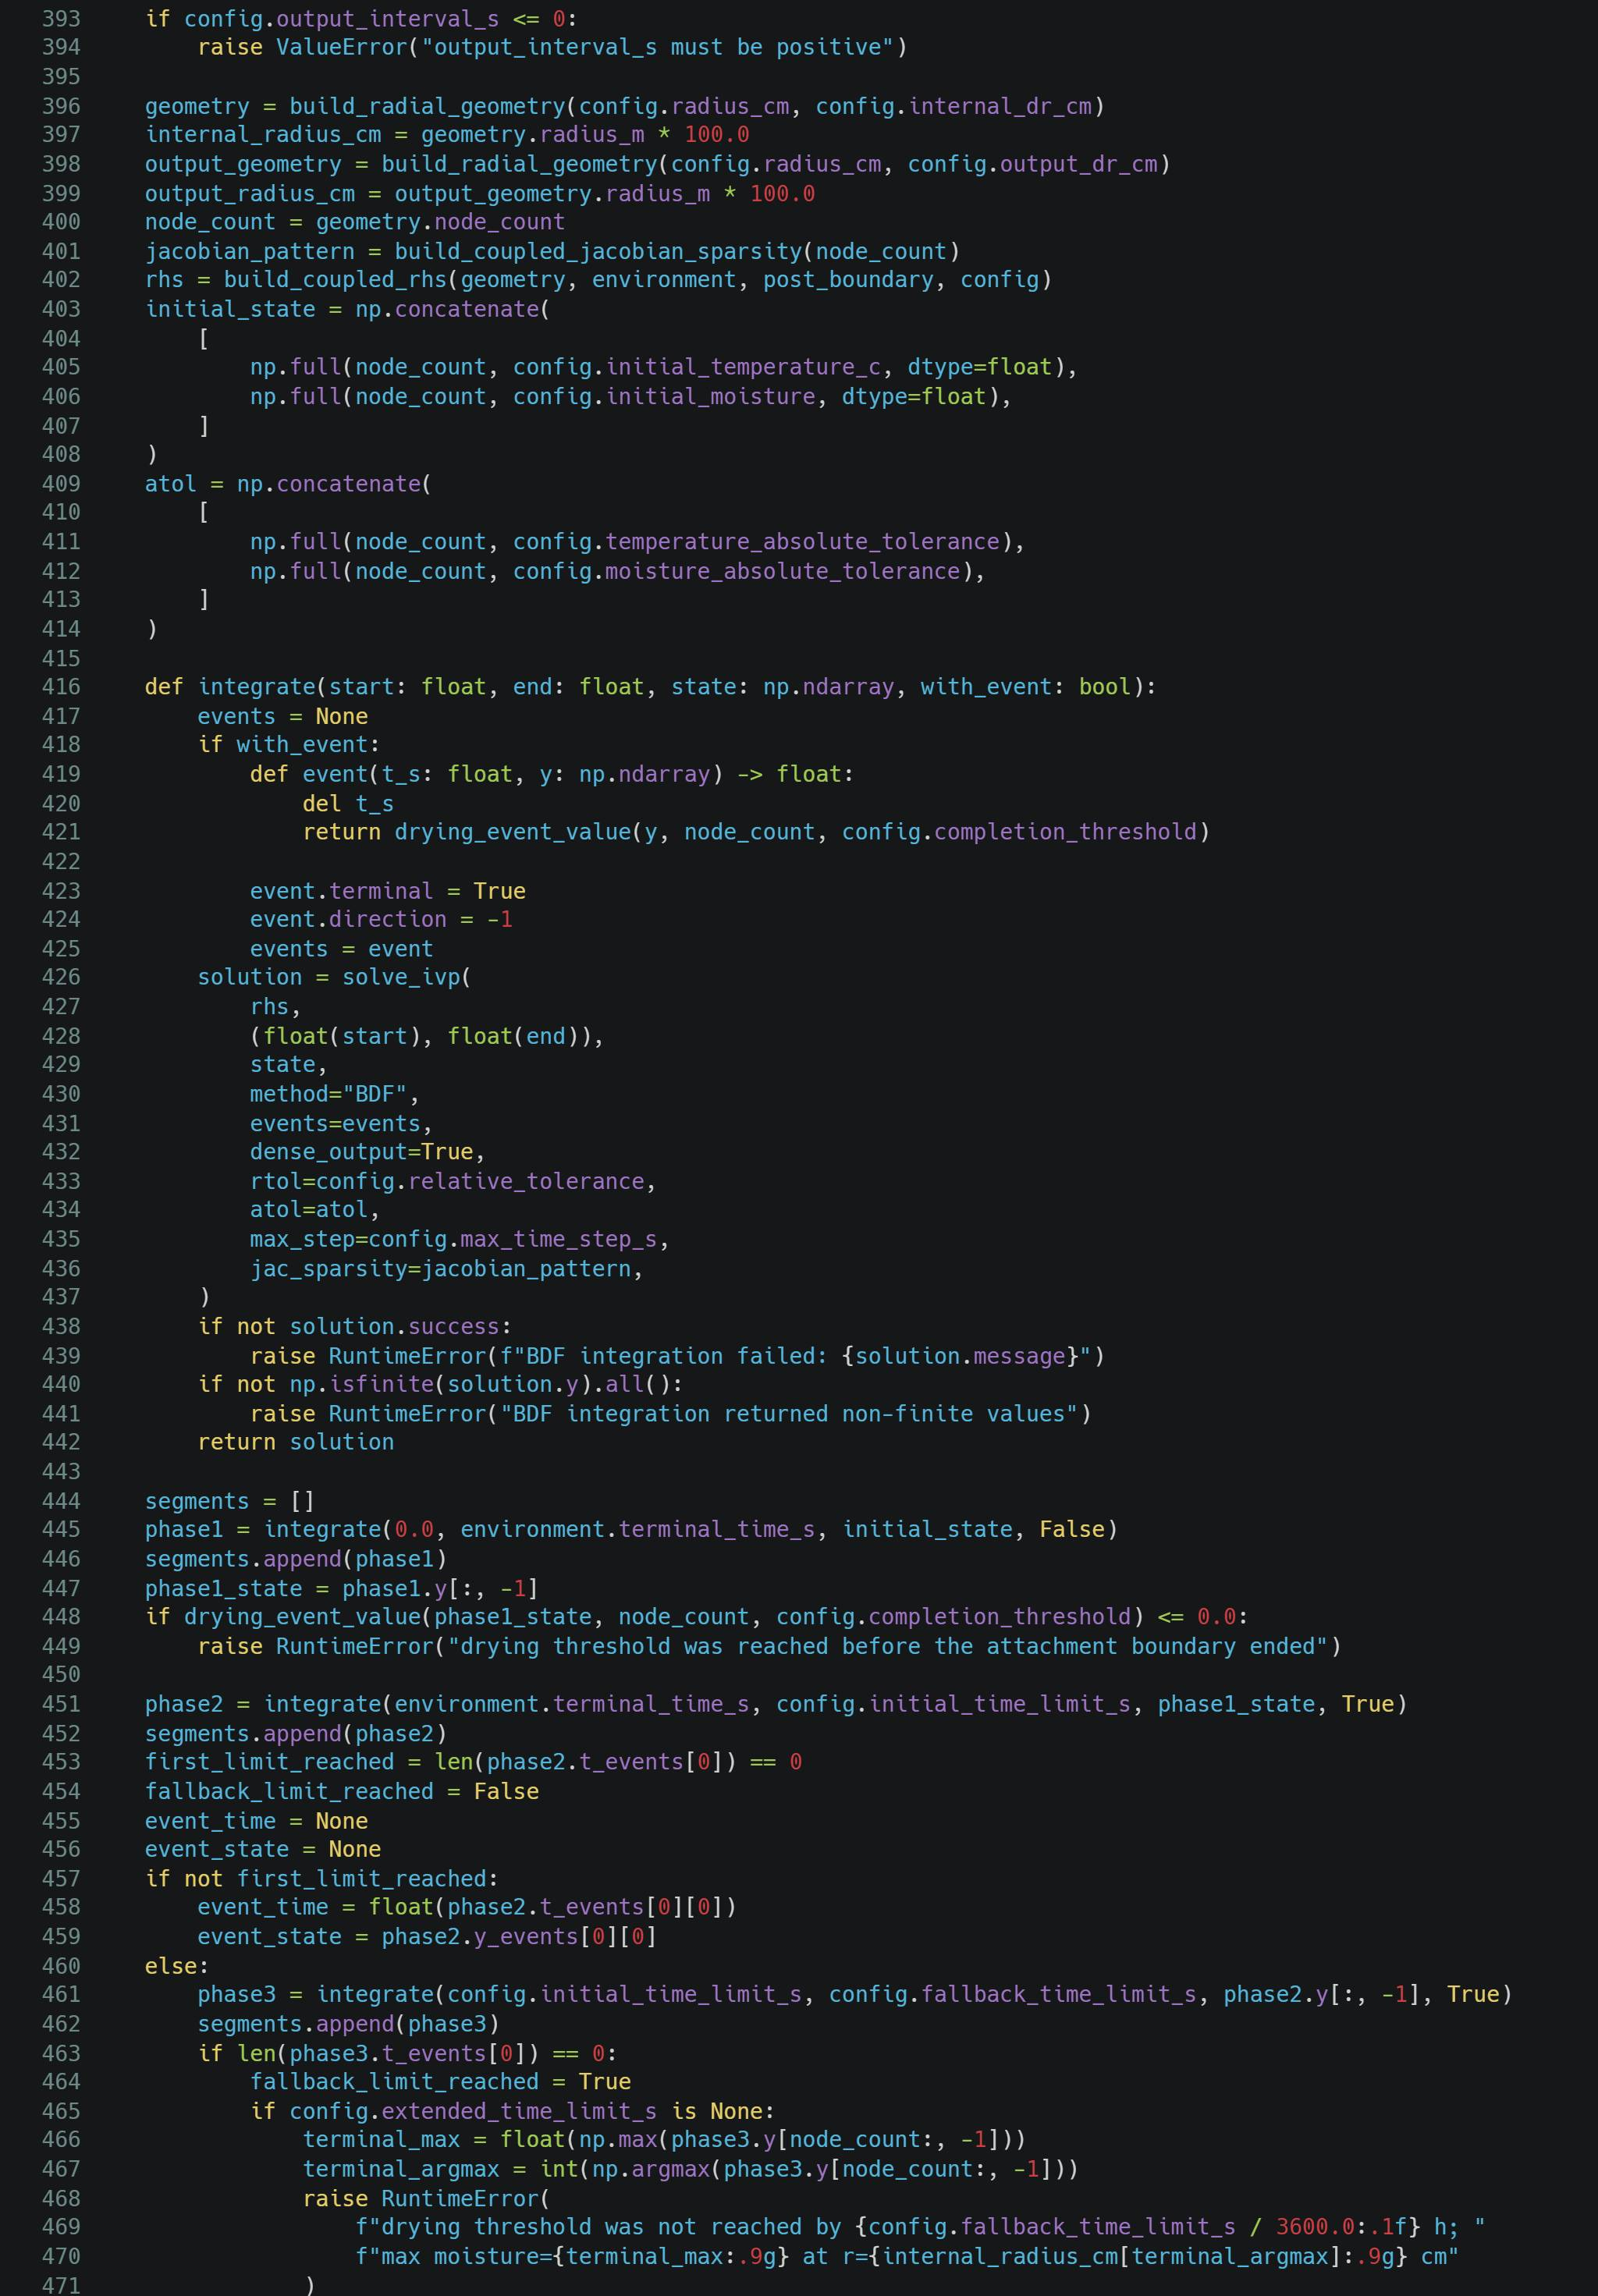
\includegraphics[width=\dimexpr\textwidth-24pt\relax]{../../code/submission/code_images/split/problem3_p6.jpg}
\newpage
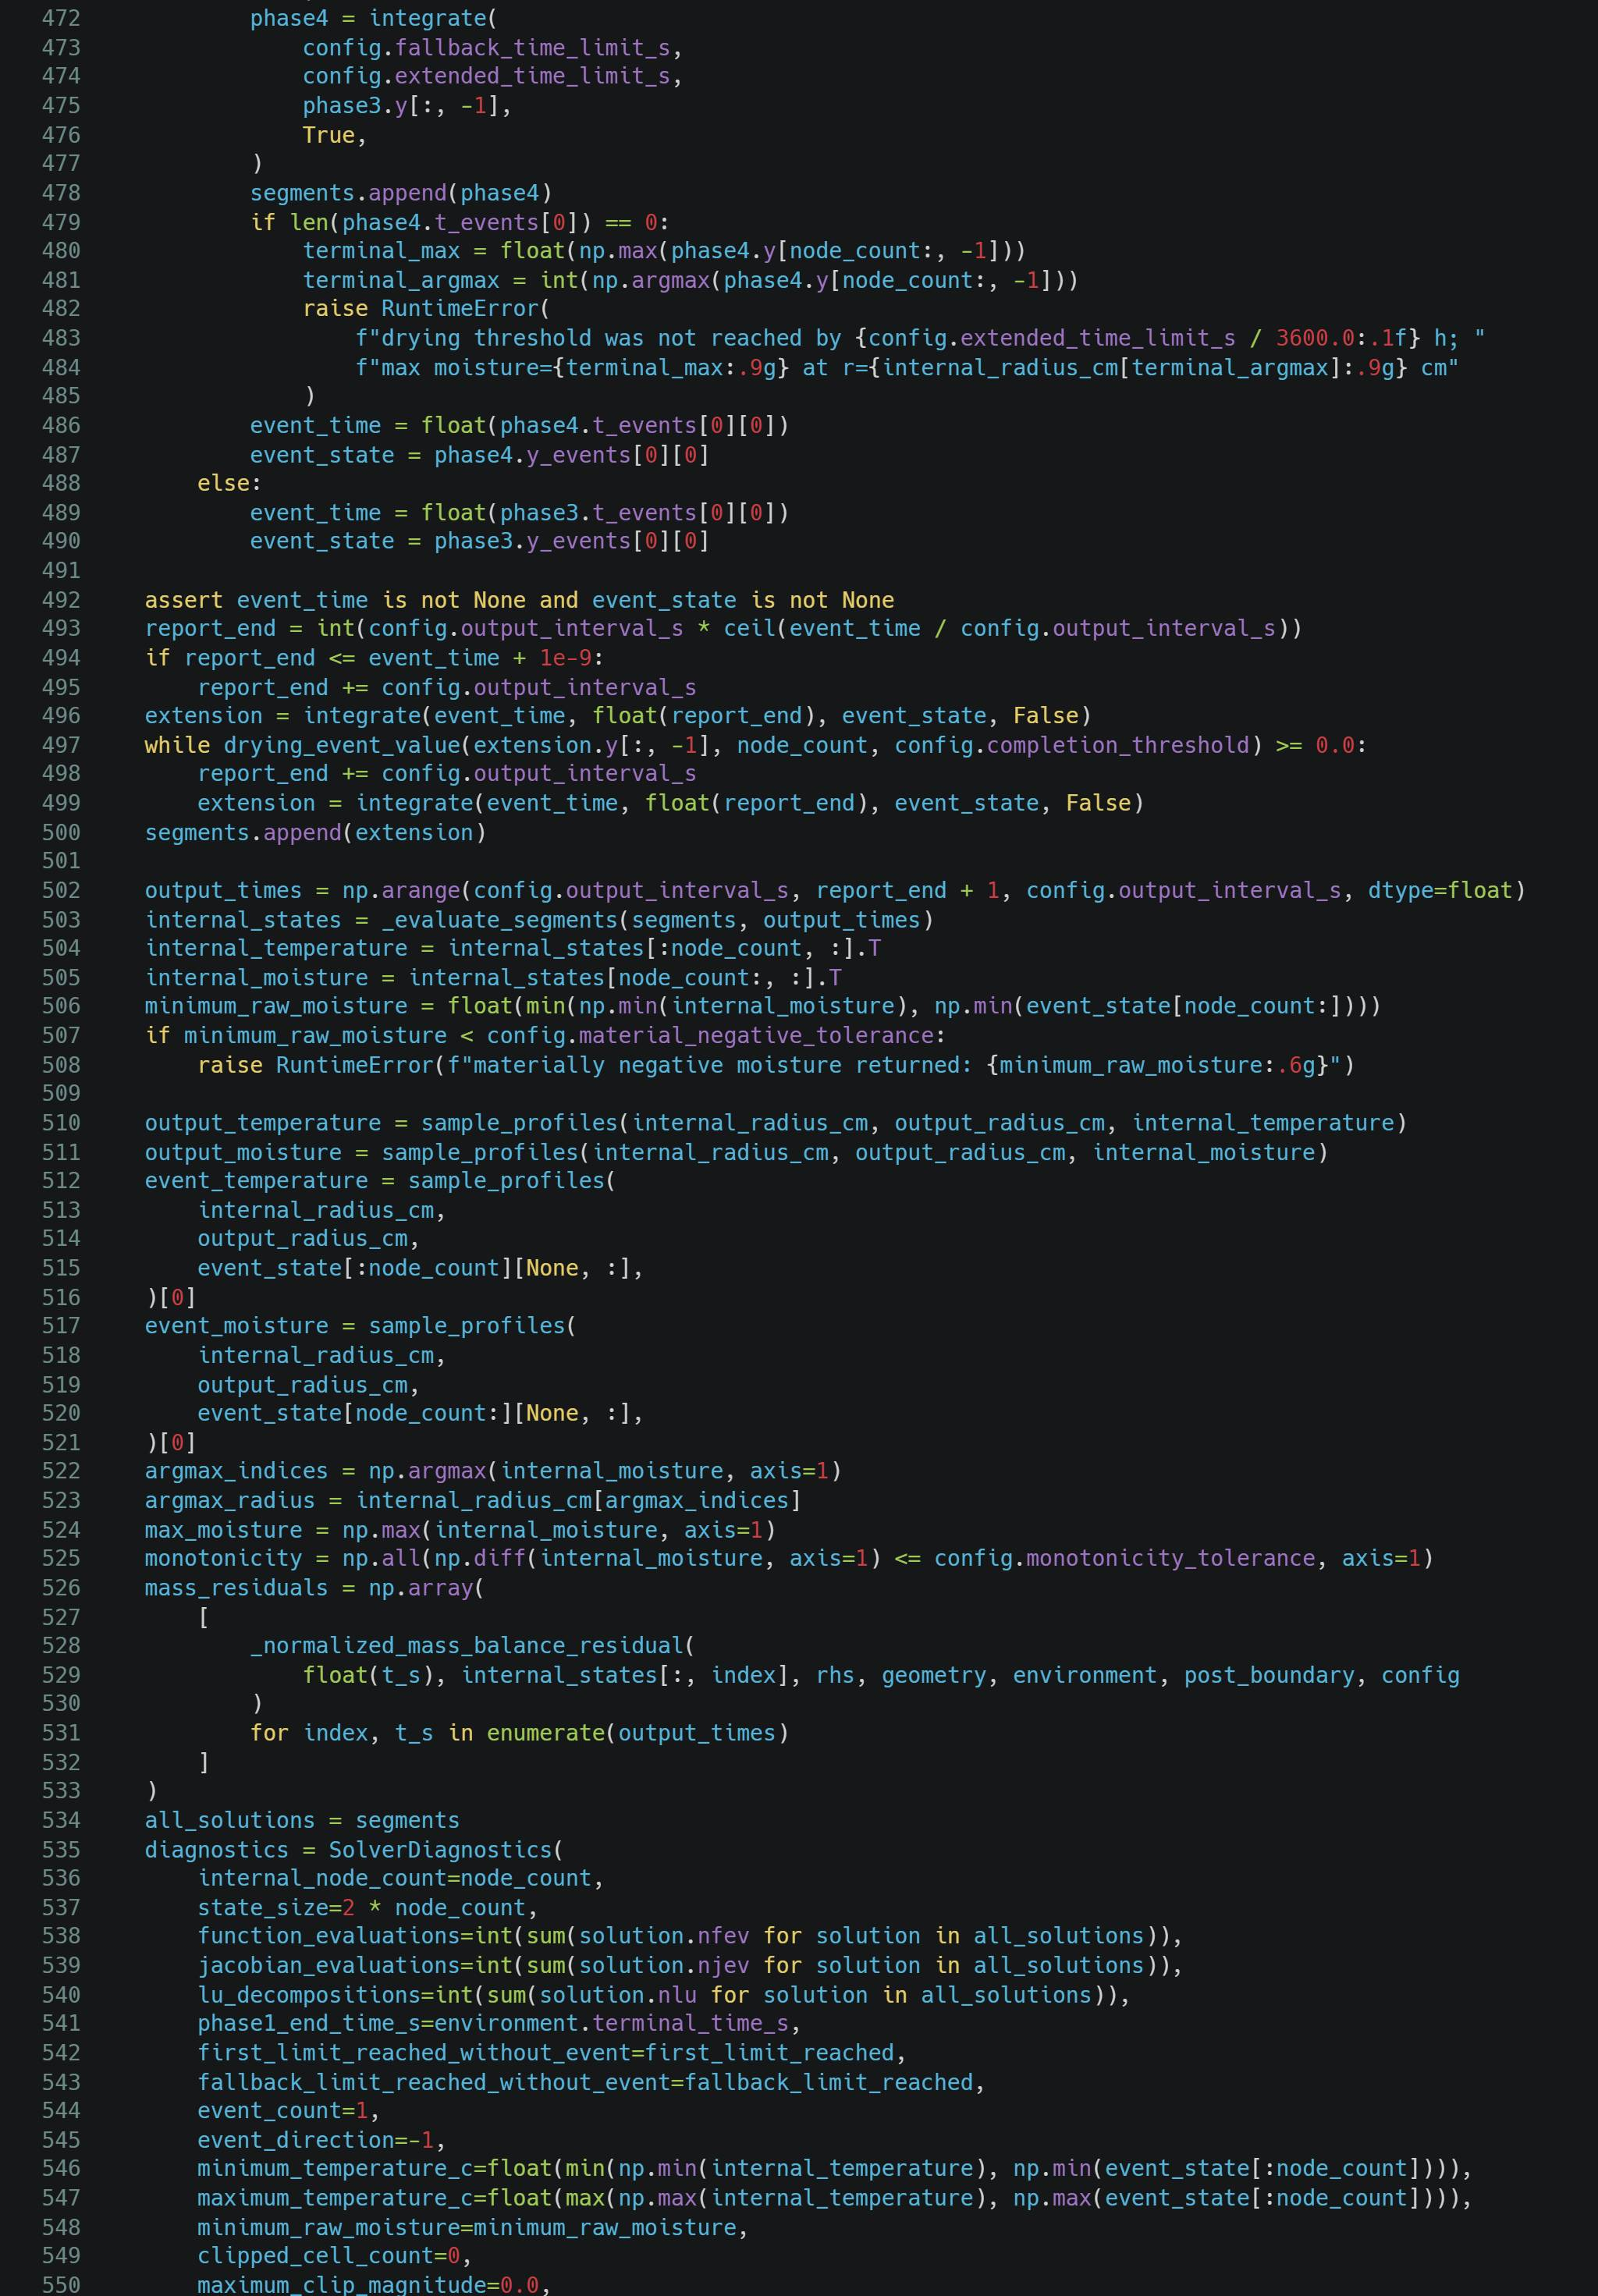
\includegraphics[width=\dimexpr\textwidth-24pt\relax]{../../code/submission/code_images/split/problem3_p7.jpg}
\newpage
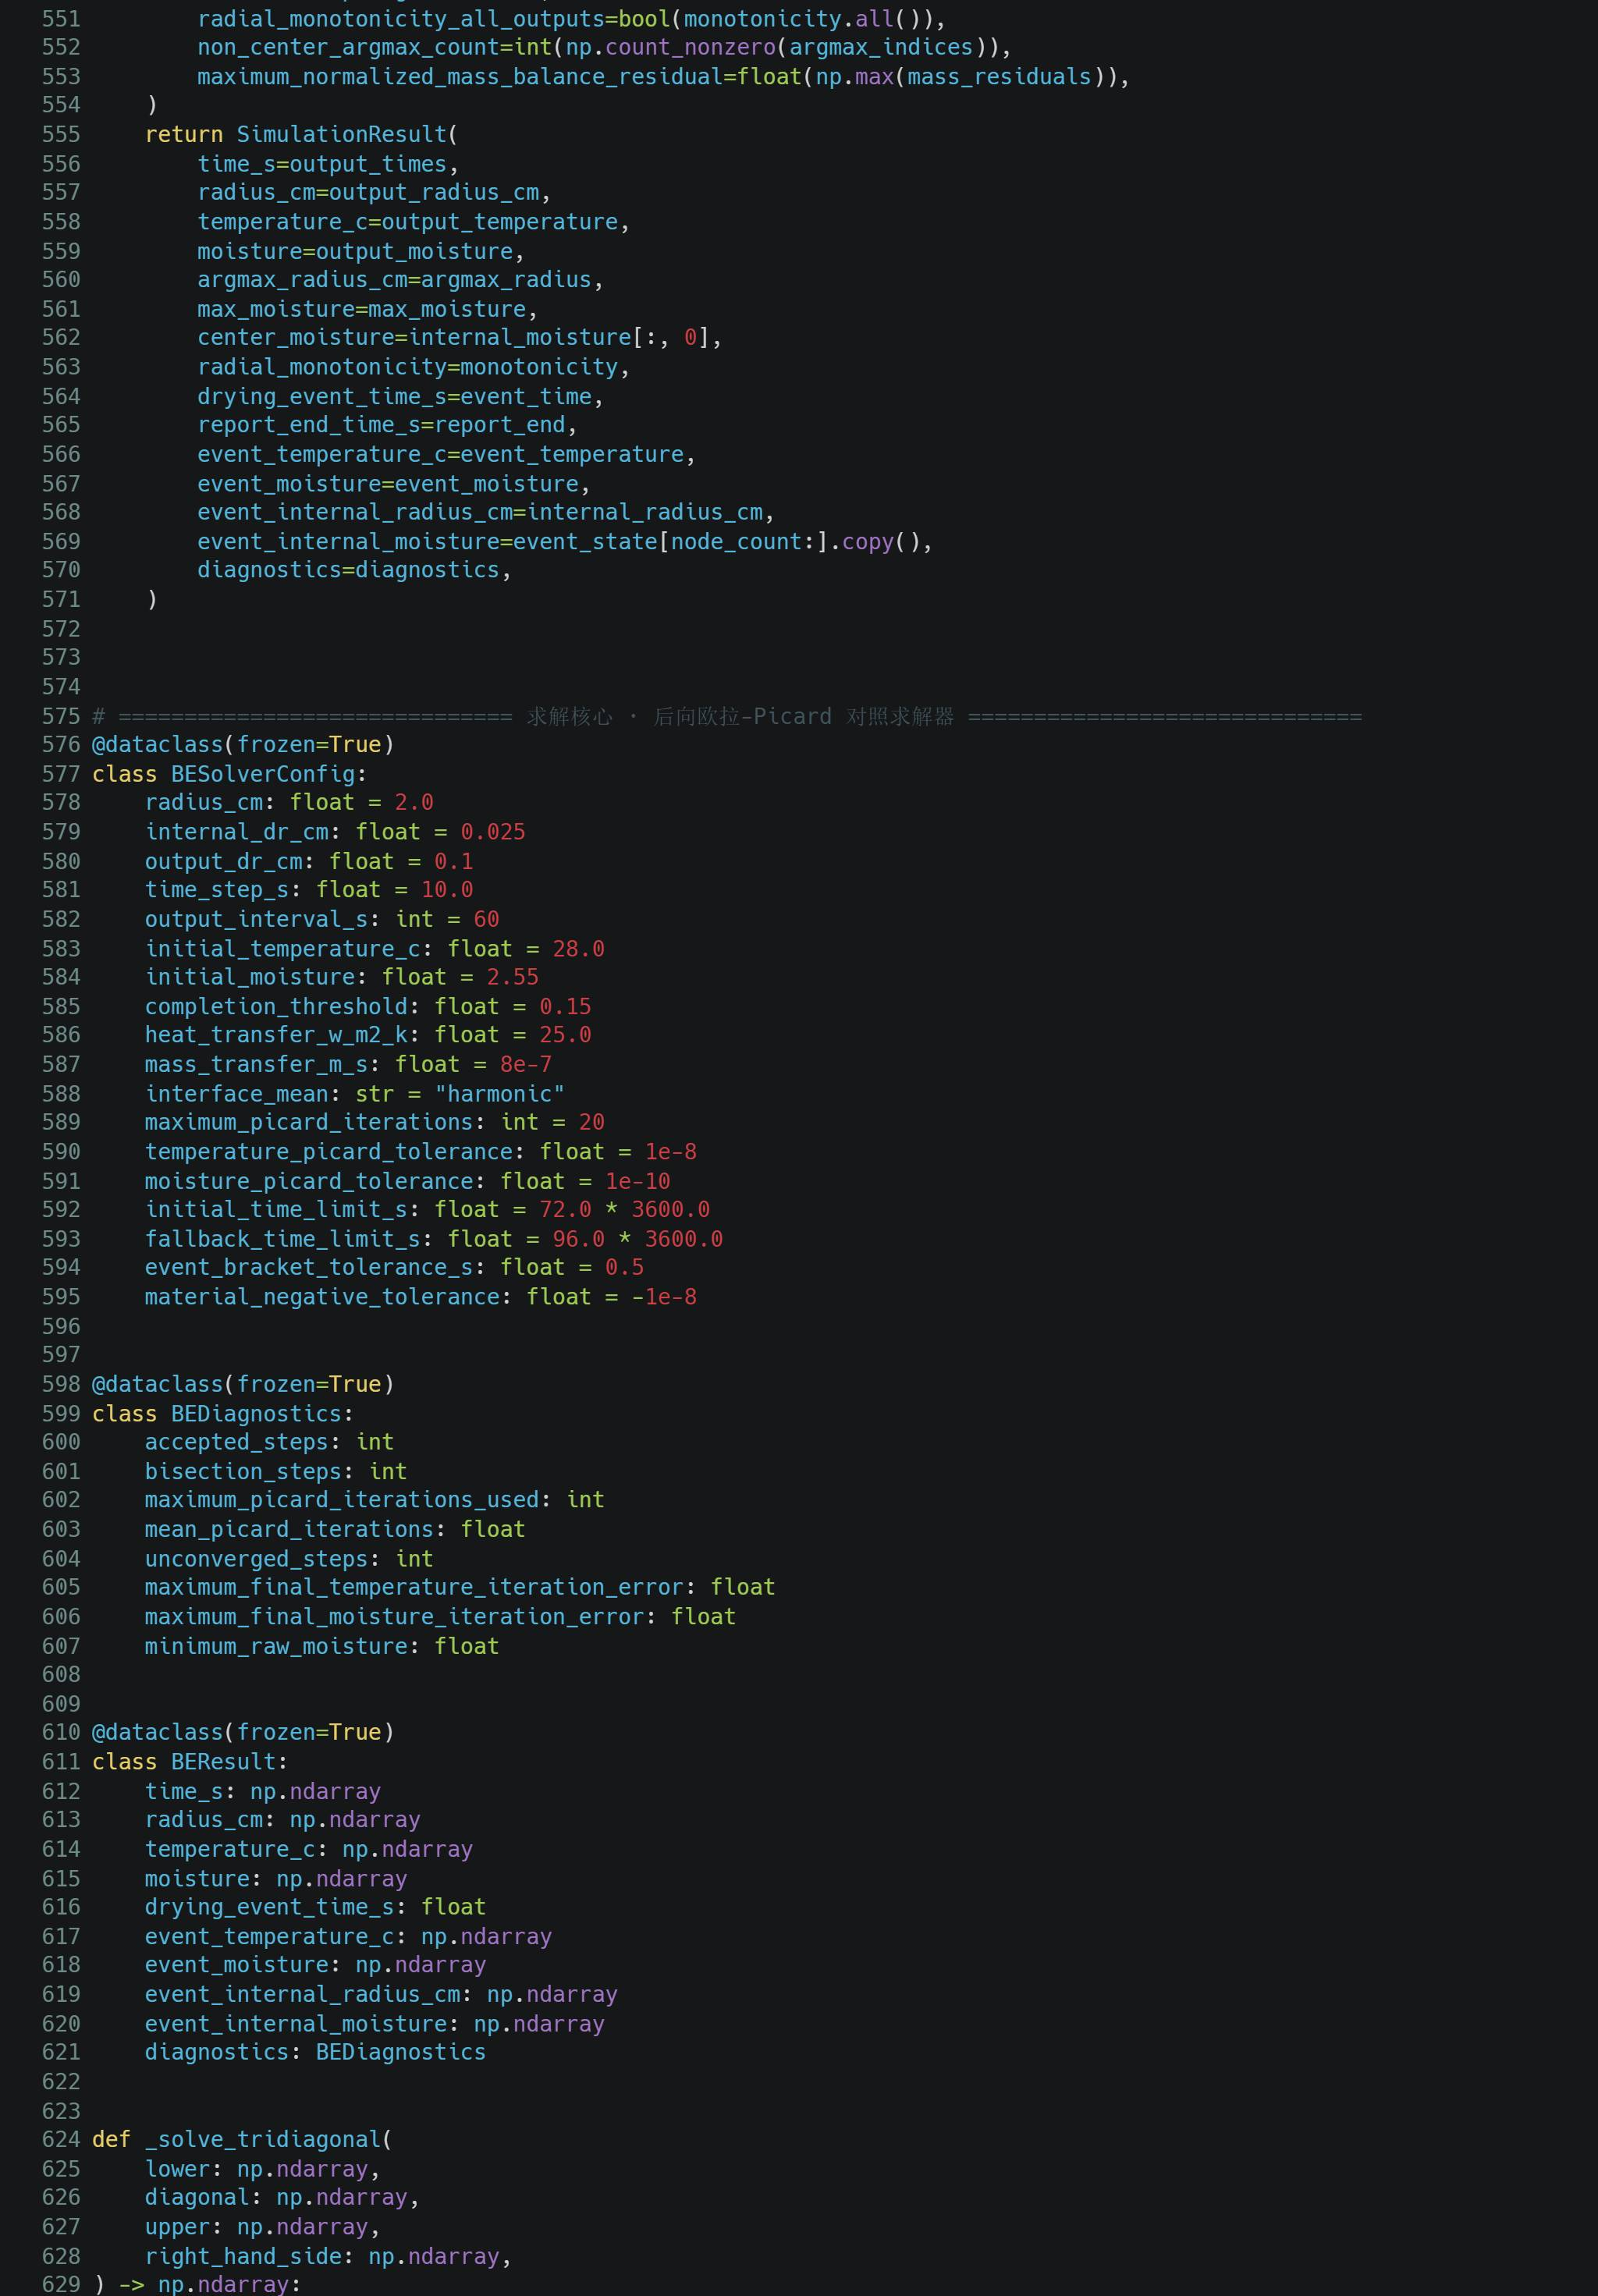
\includegraphics[width=\dimexpr\textwidth-24pt\relax]{../../code/submission/code_images/split/problem3_p8.jpg}
\newpage
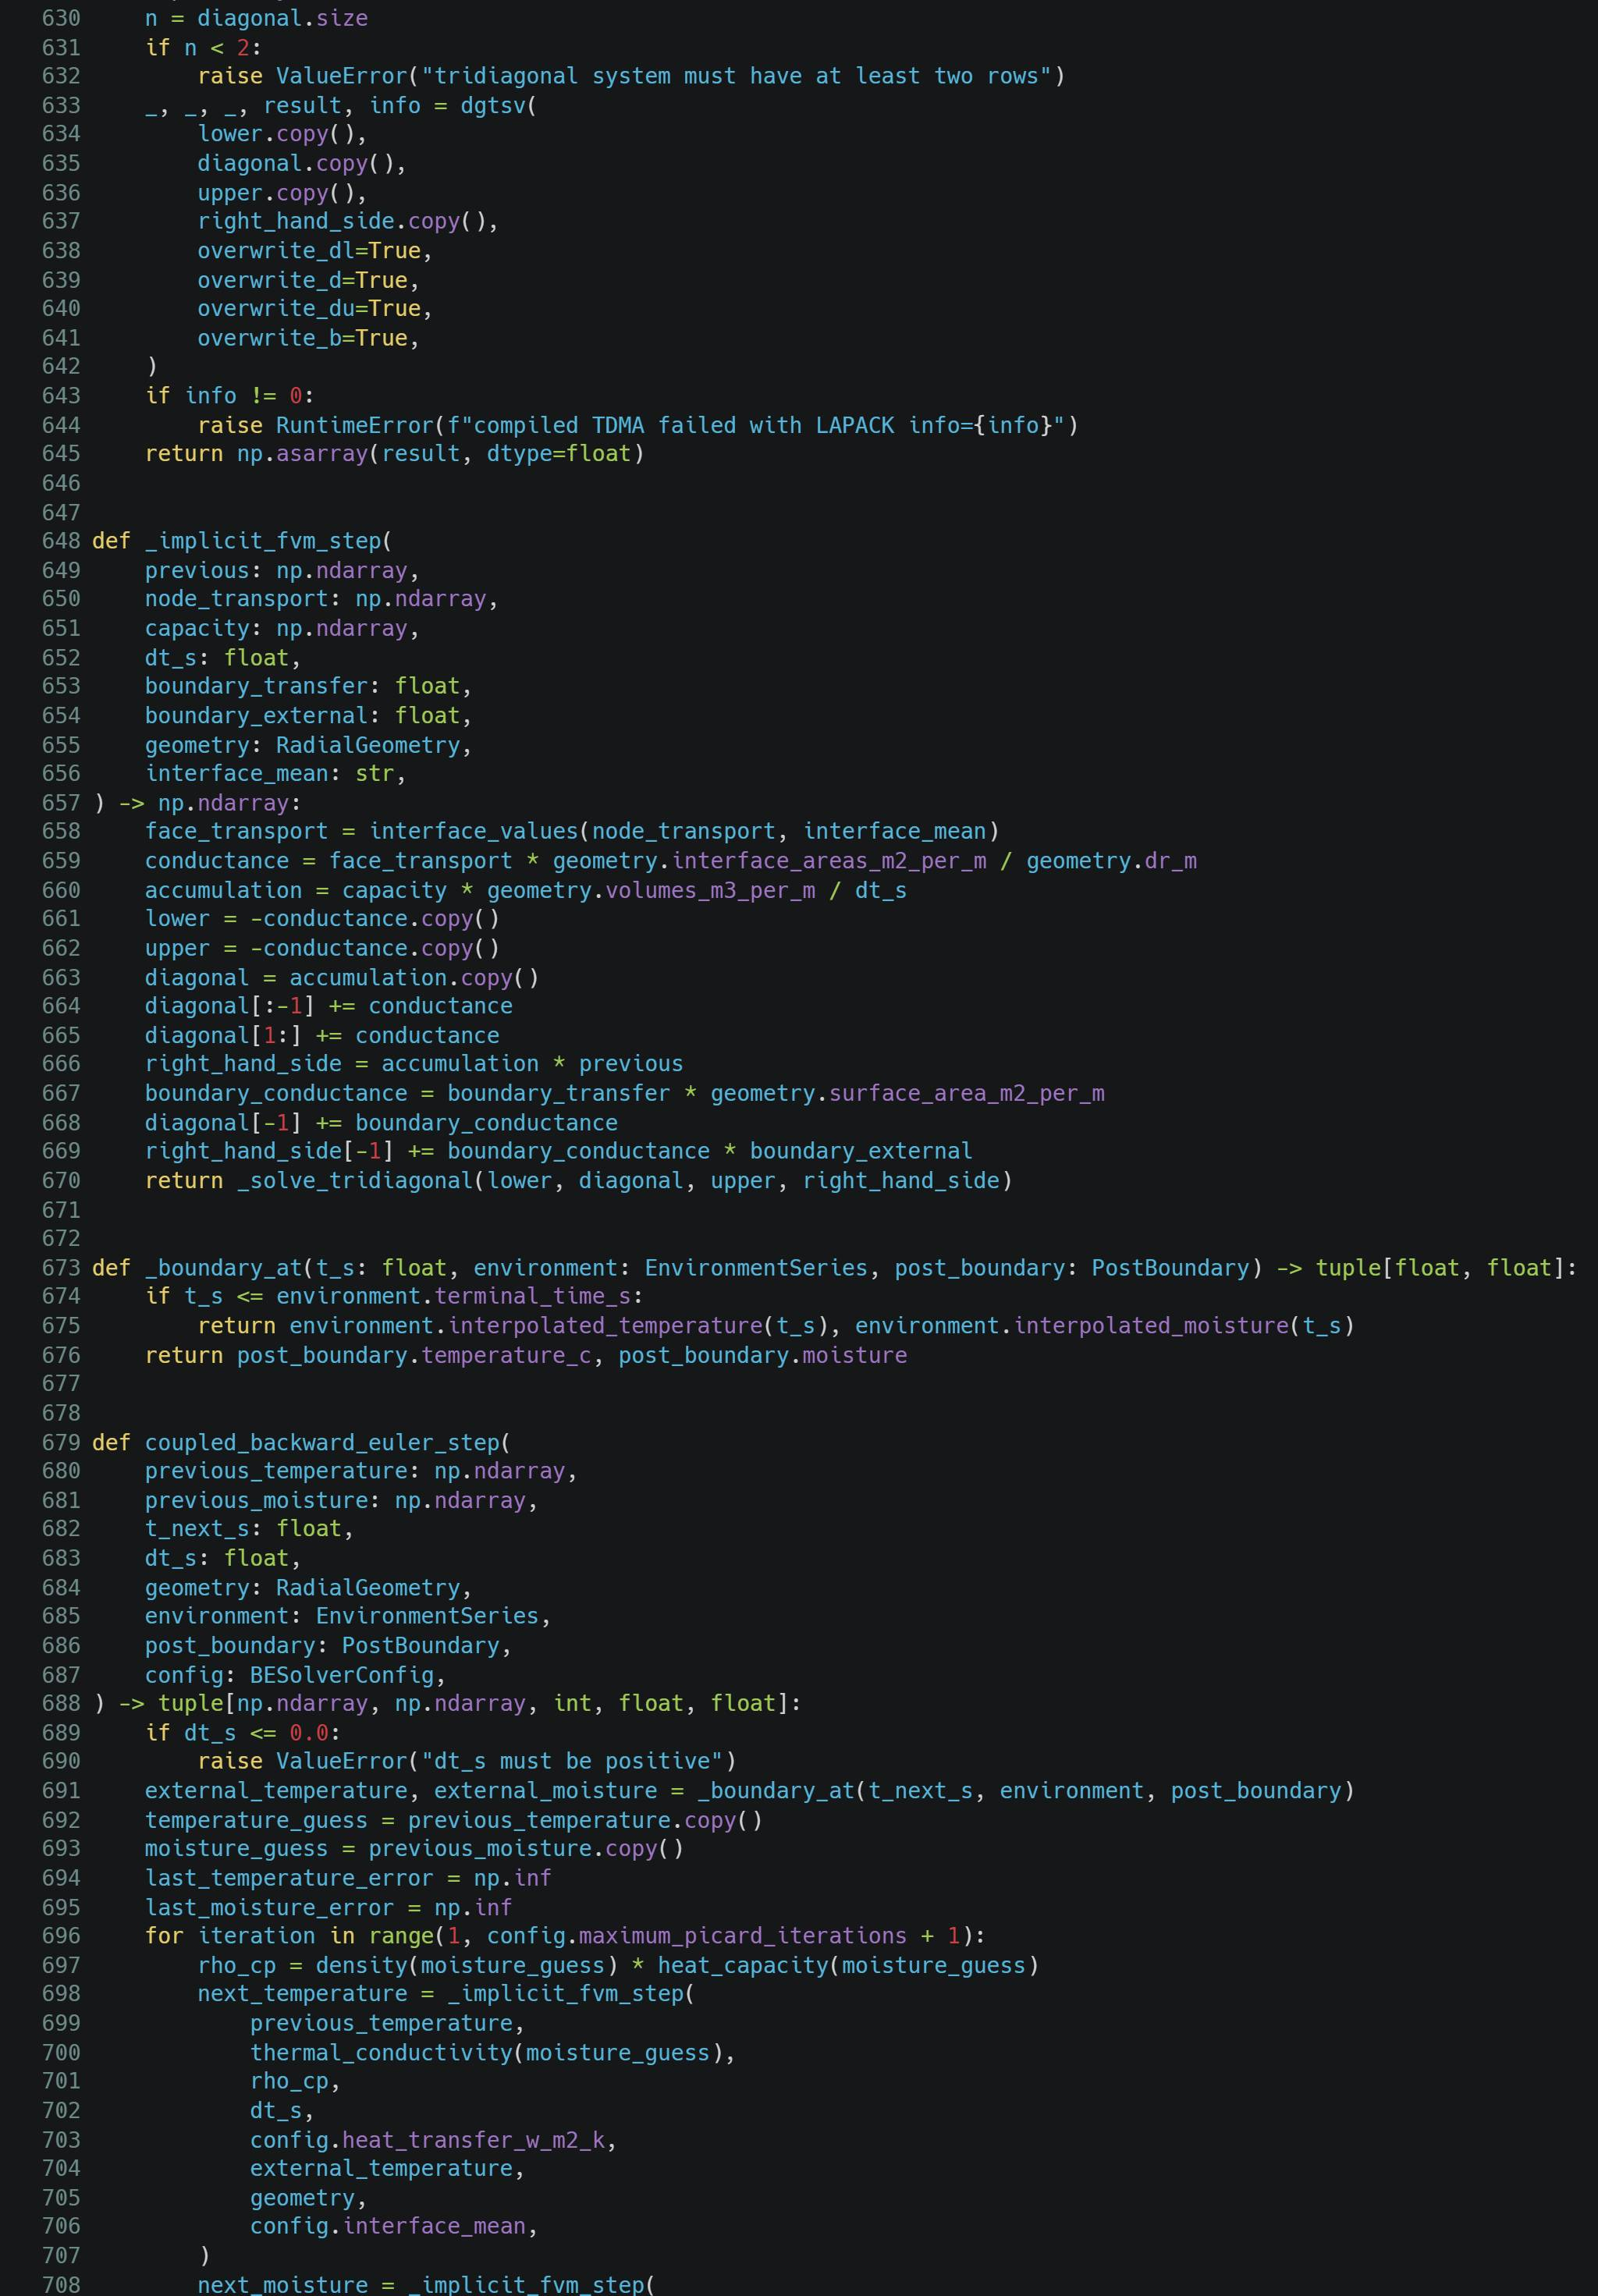
\includegraphics[width=\dimexpr\textwidth-24pt\relax]{../../code/submission/code_images/split/problem3_p9.jpg}
\newpage
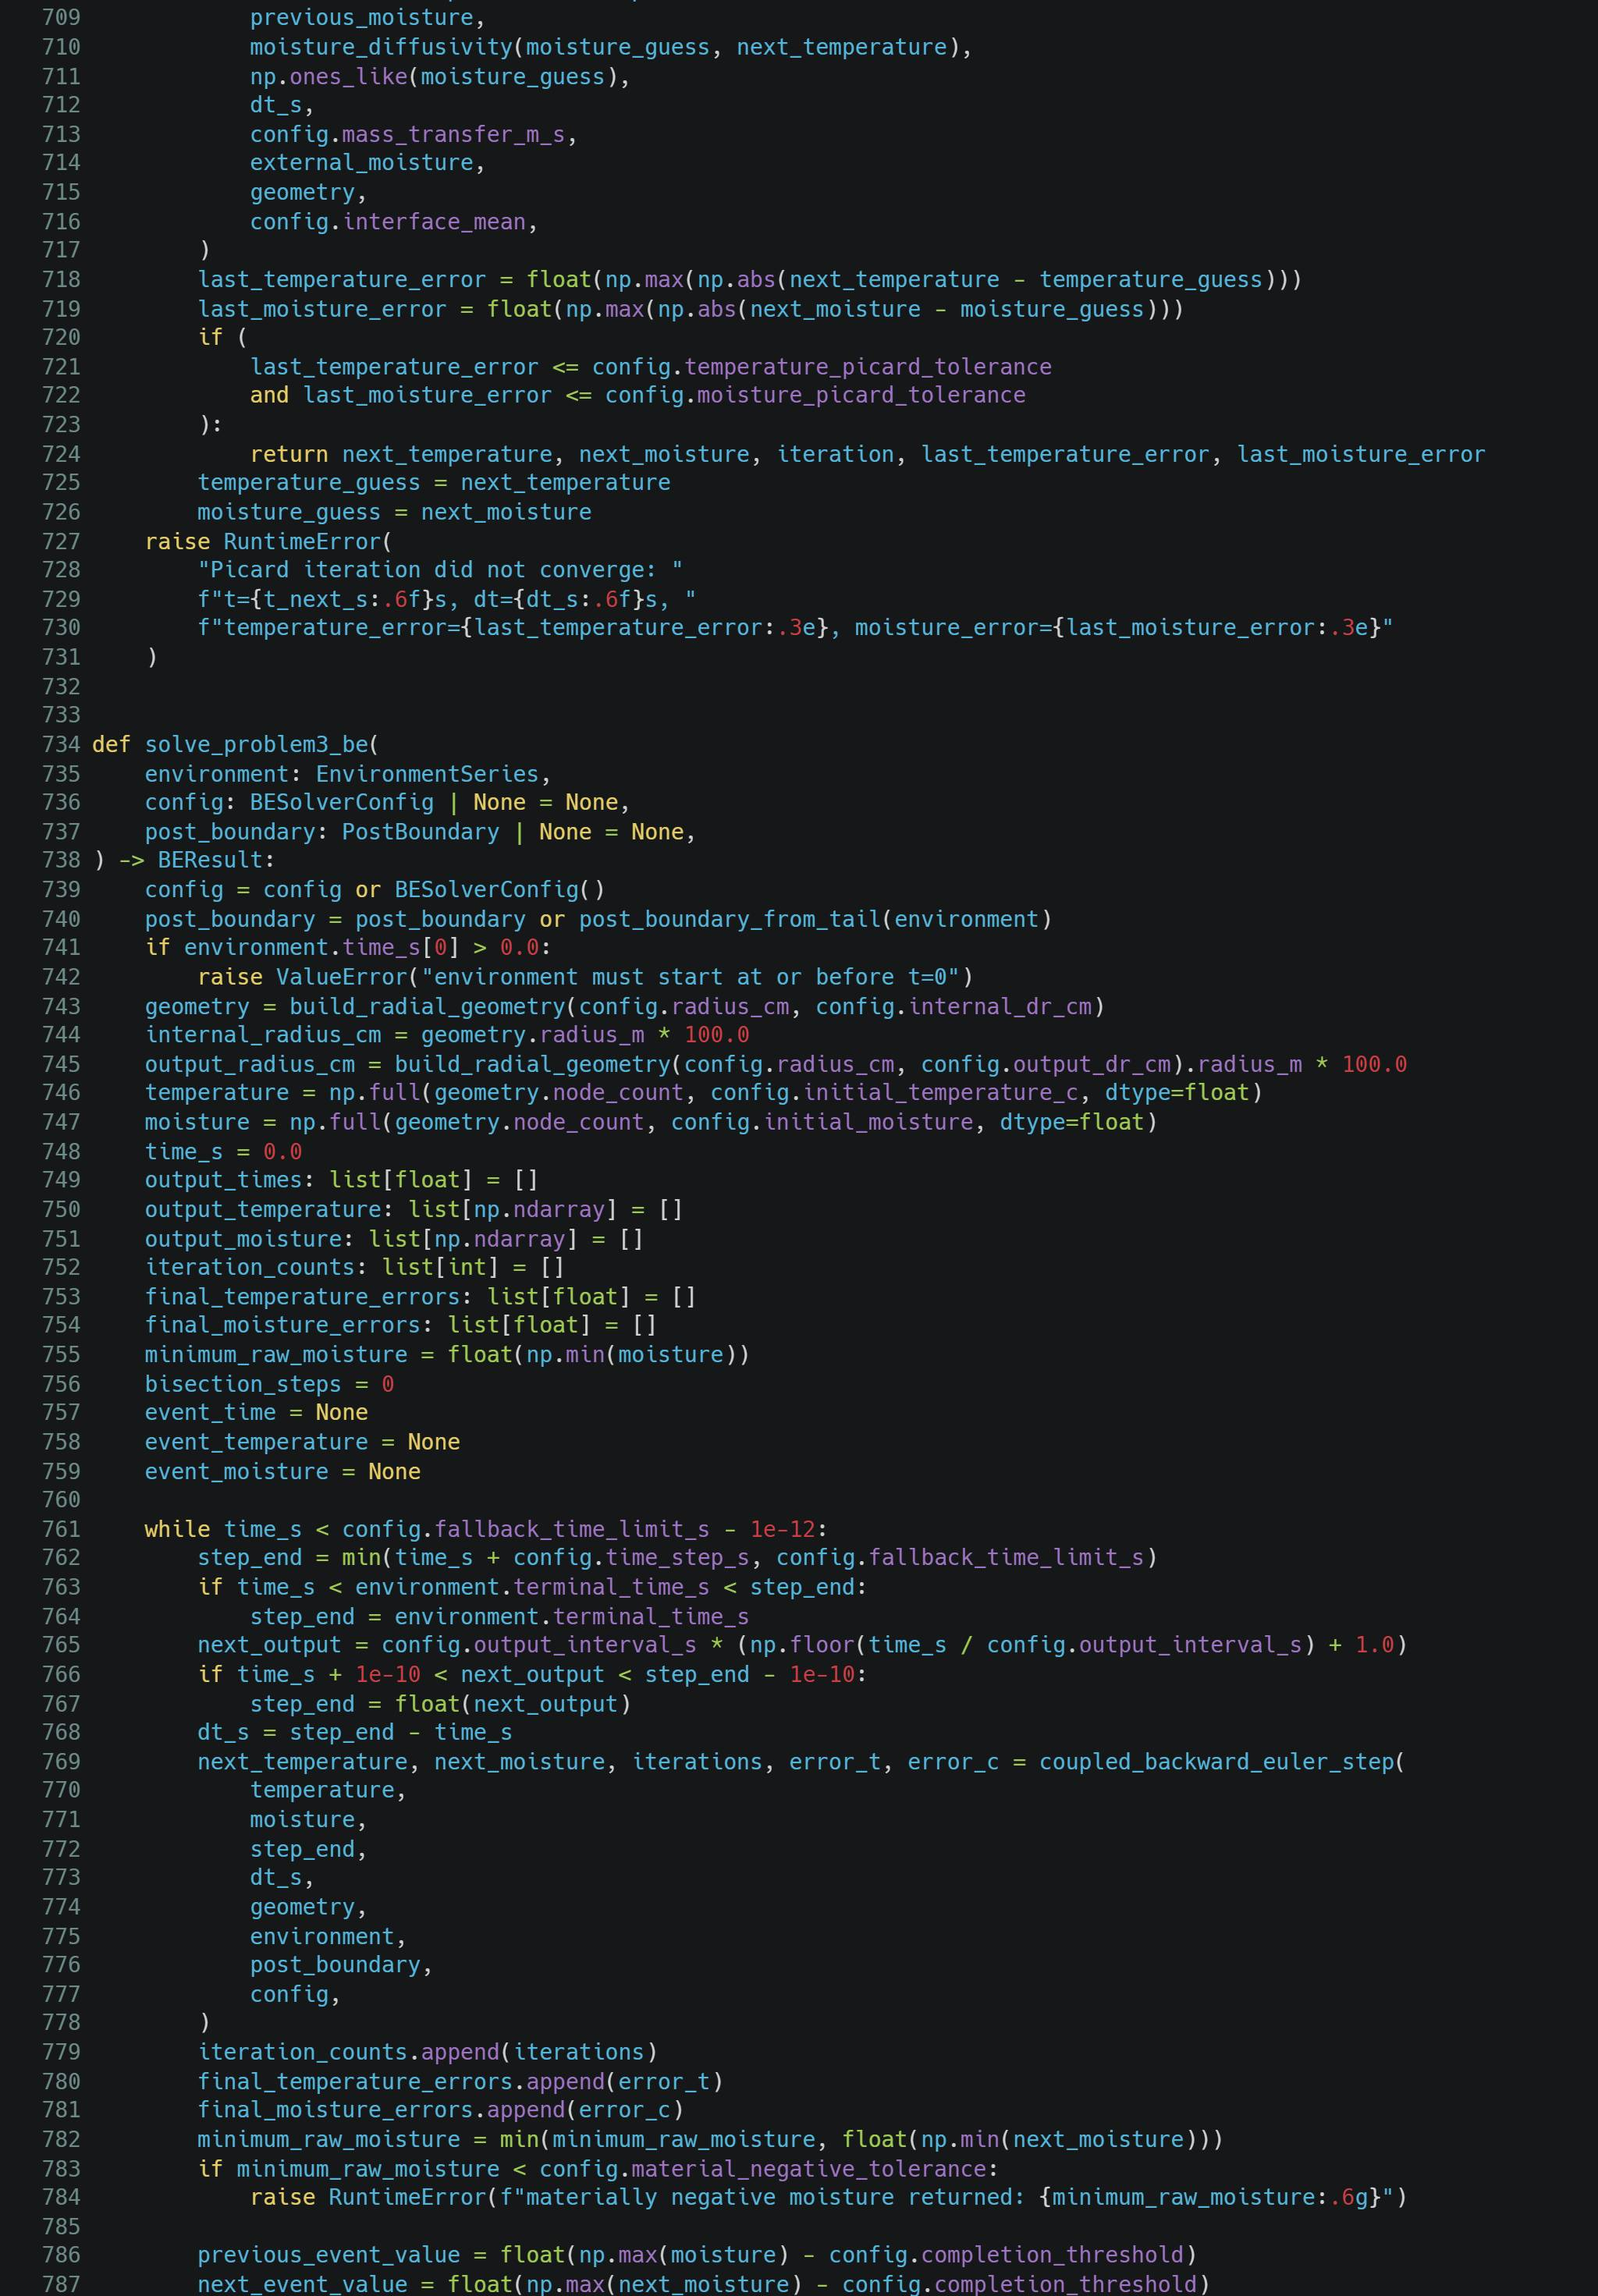
\includegraphics[width=\dimexpr\textwidth-24pt\relax]{../../code/submission/code_images/split/problem3_p10.jpg}
\newpage
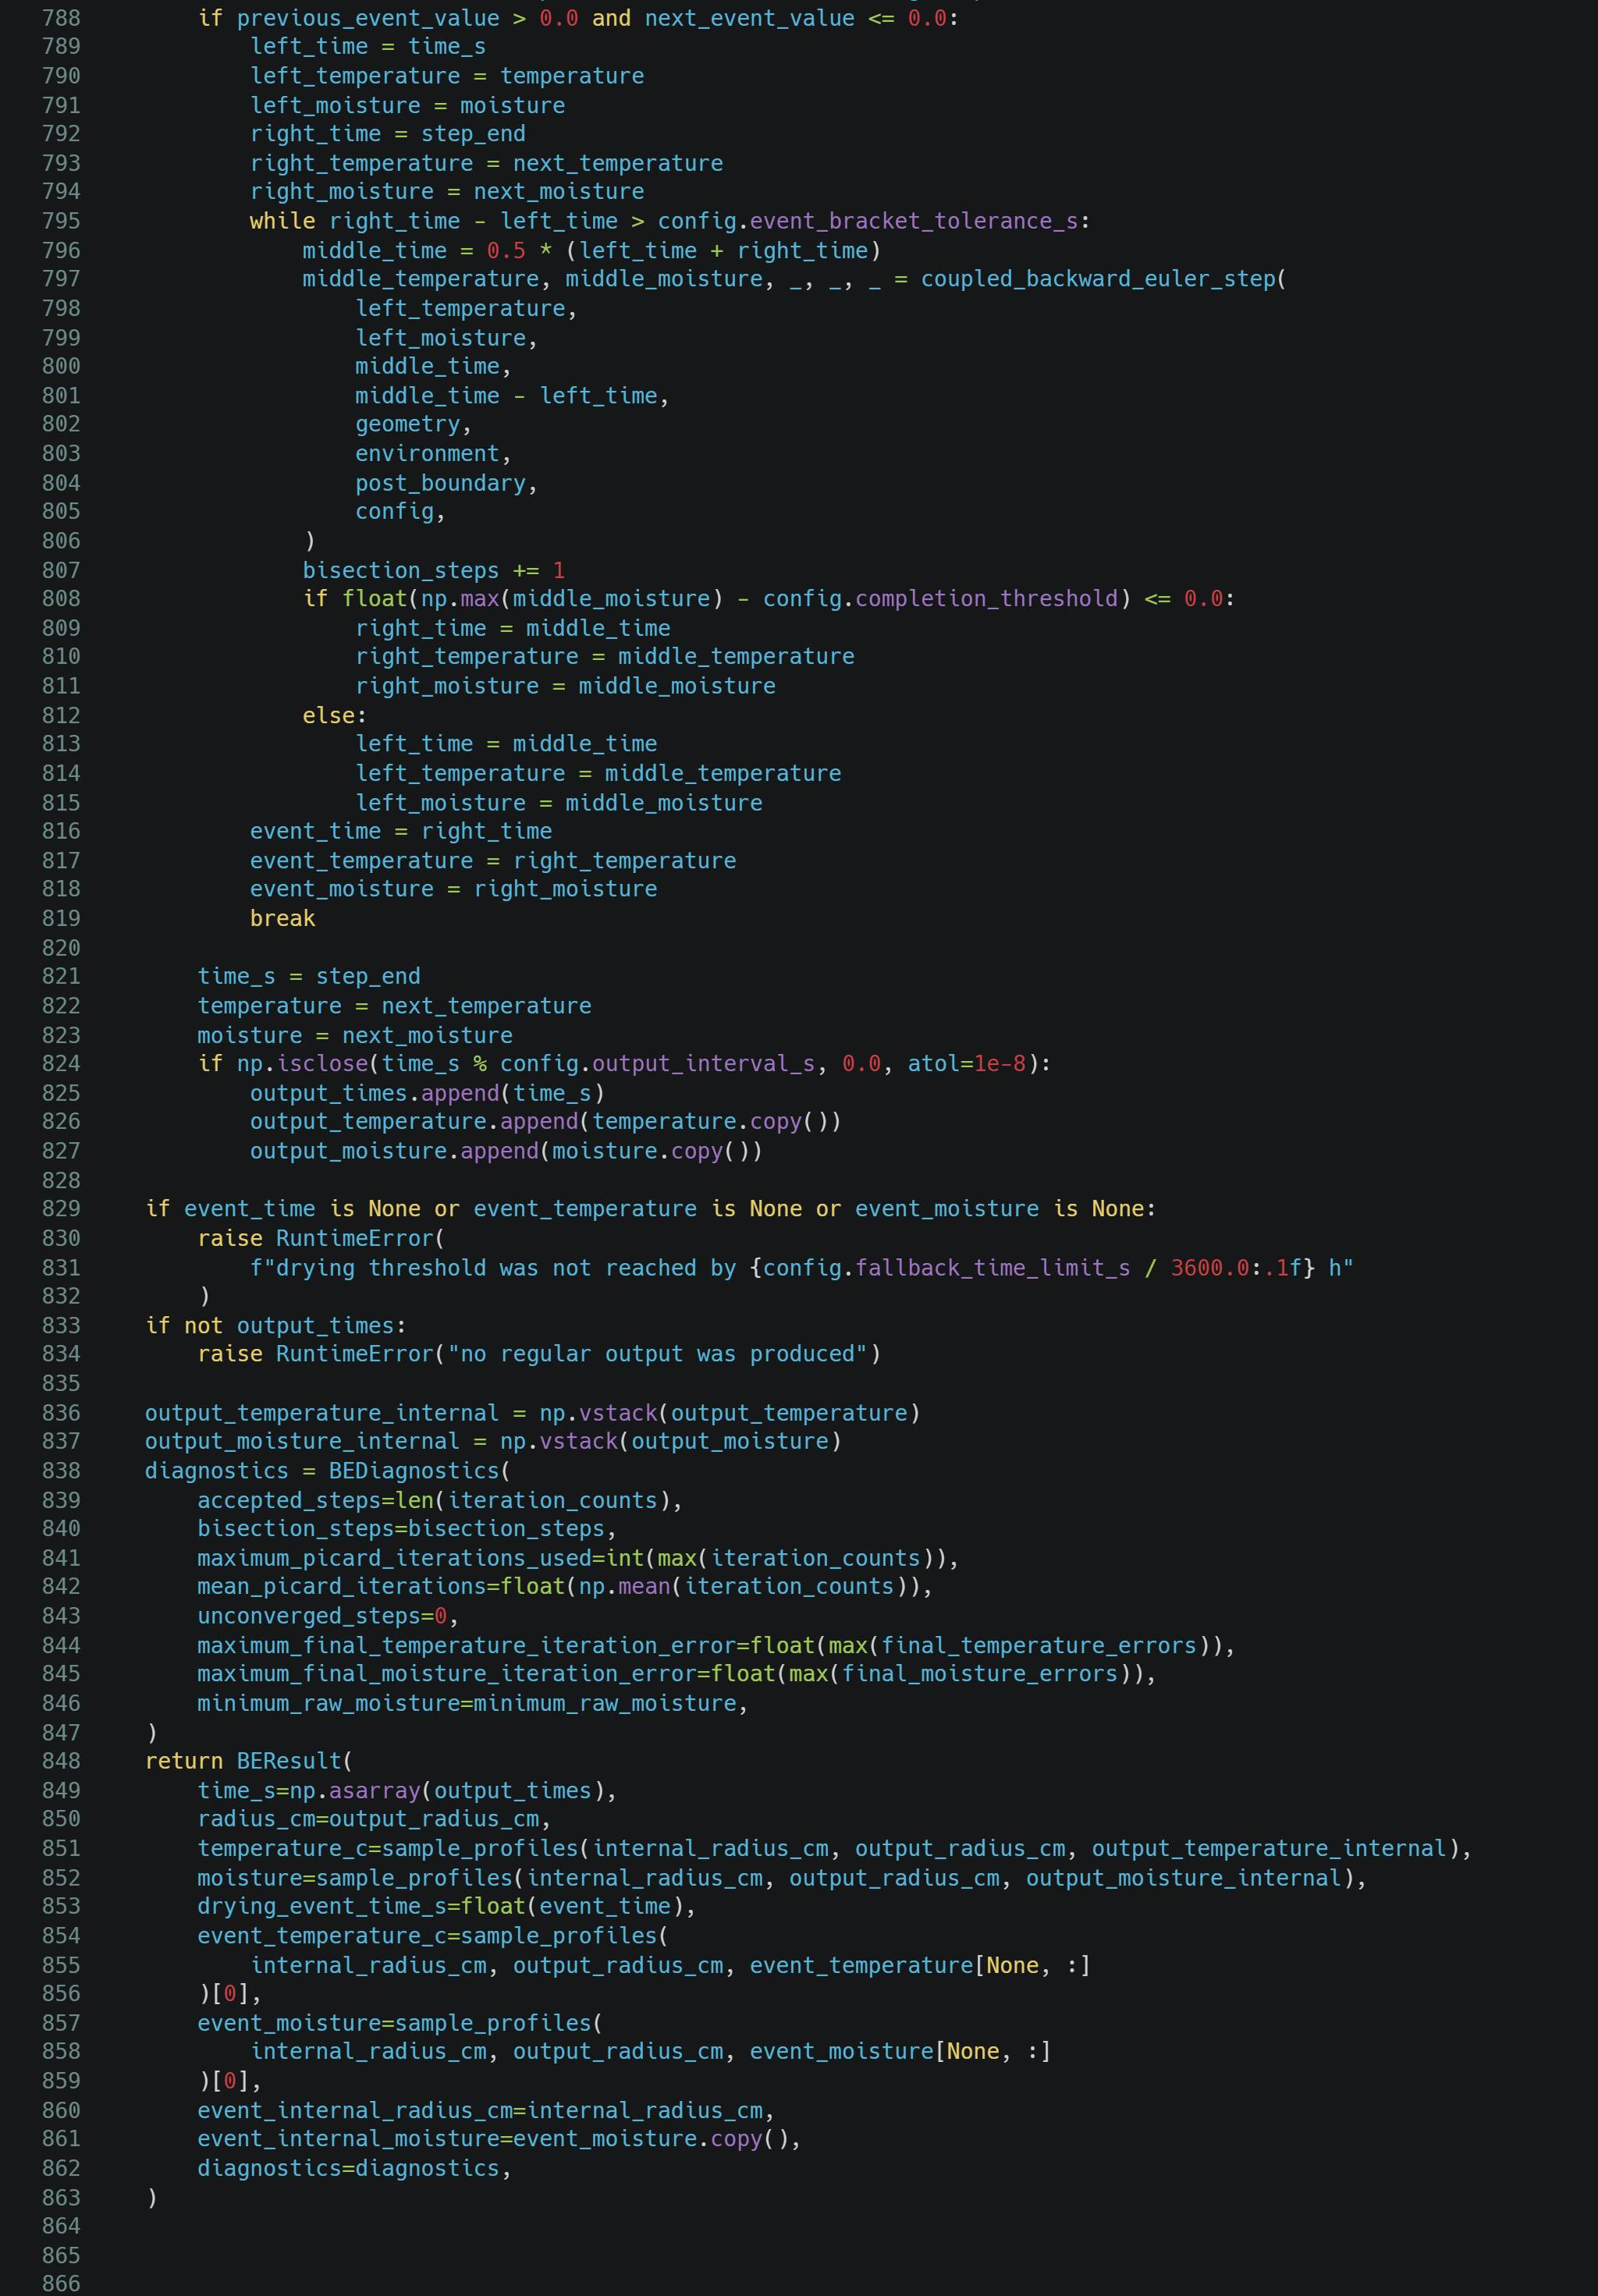
\includegraphics[width=\dimexpr\textwidth-24pt\relax]{../../code/submission/code_images/split/problem3_p11.jpg}
\newpage
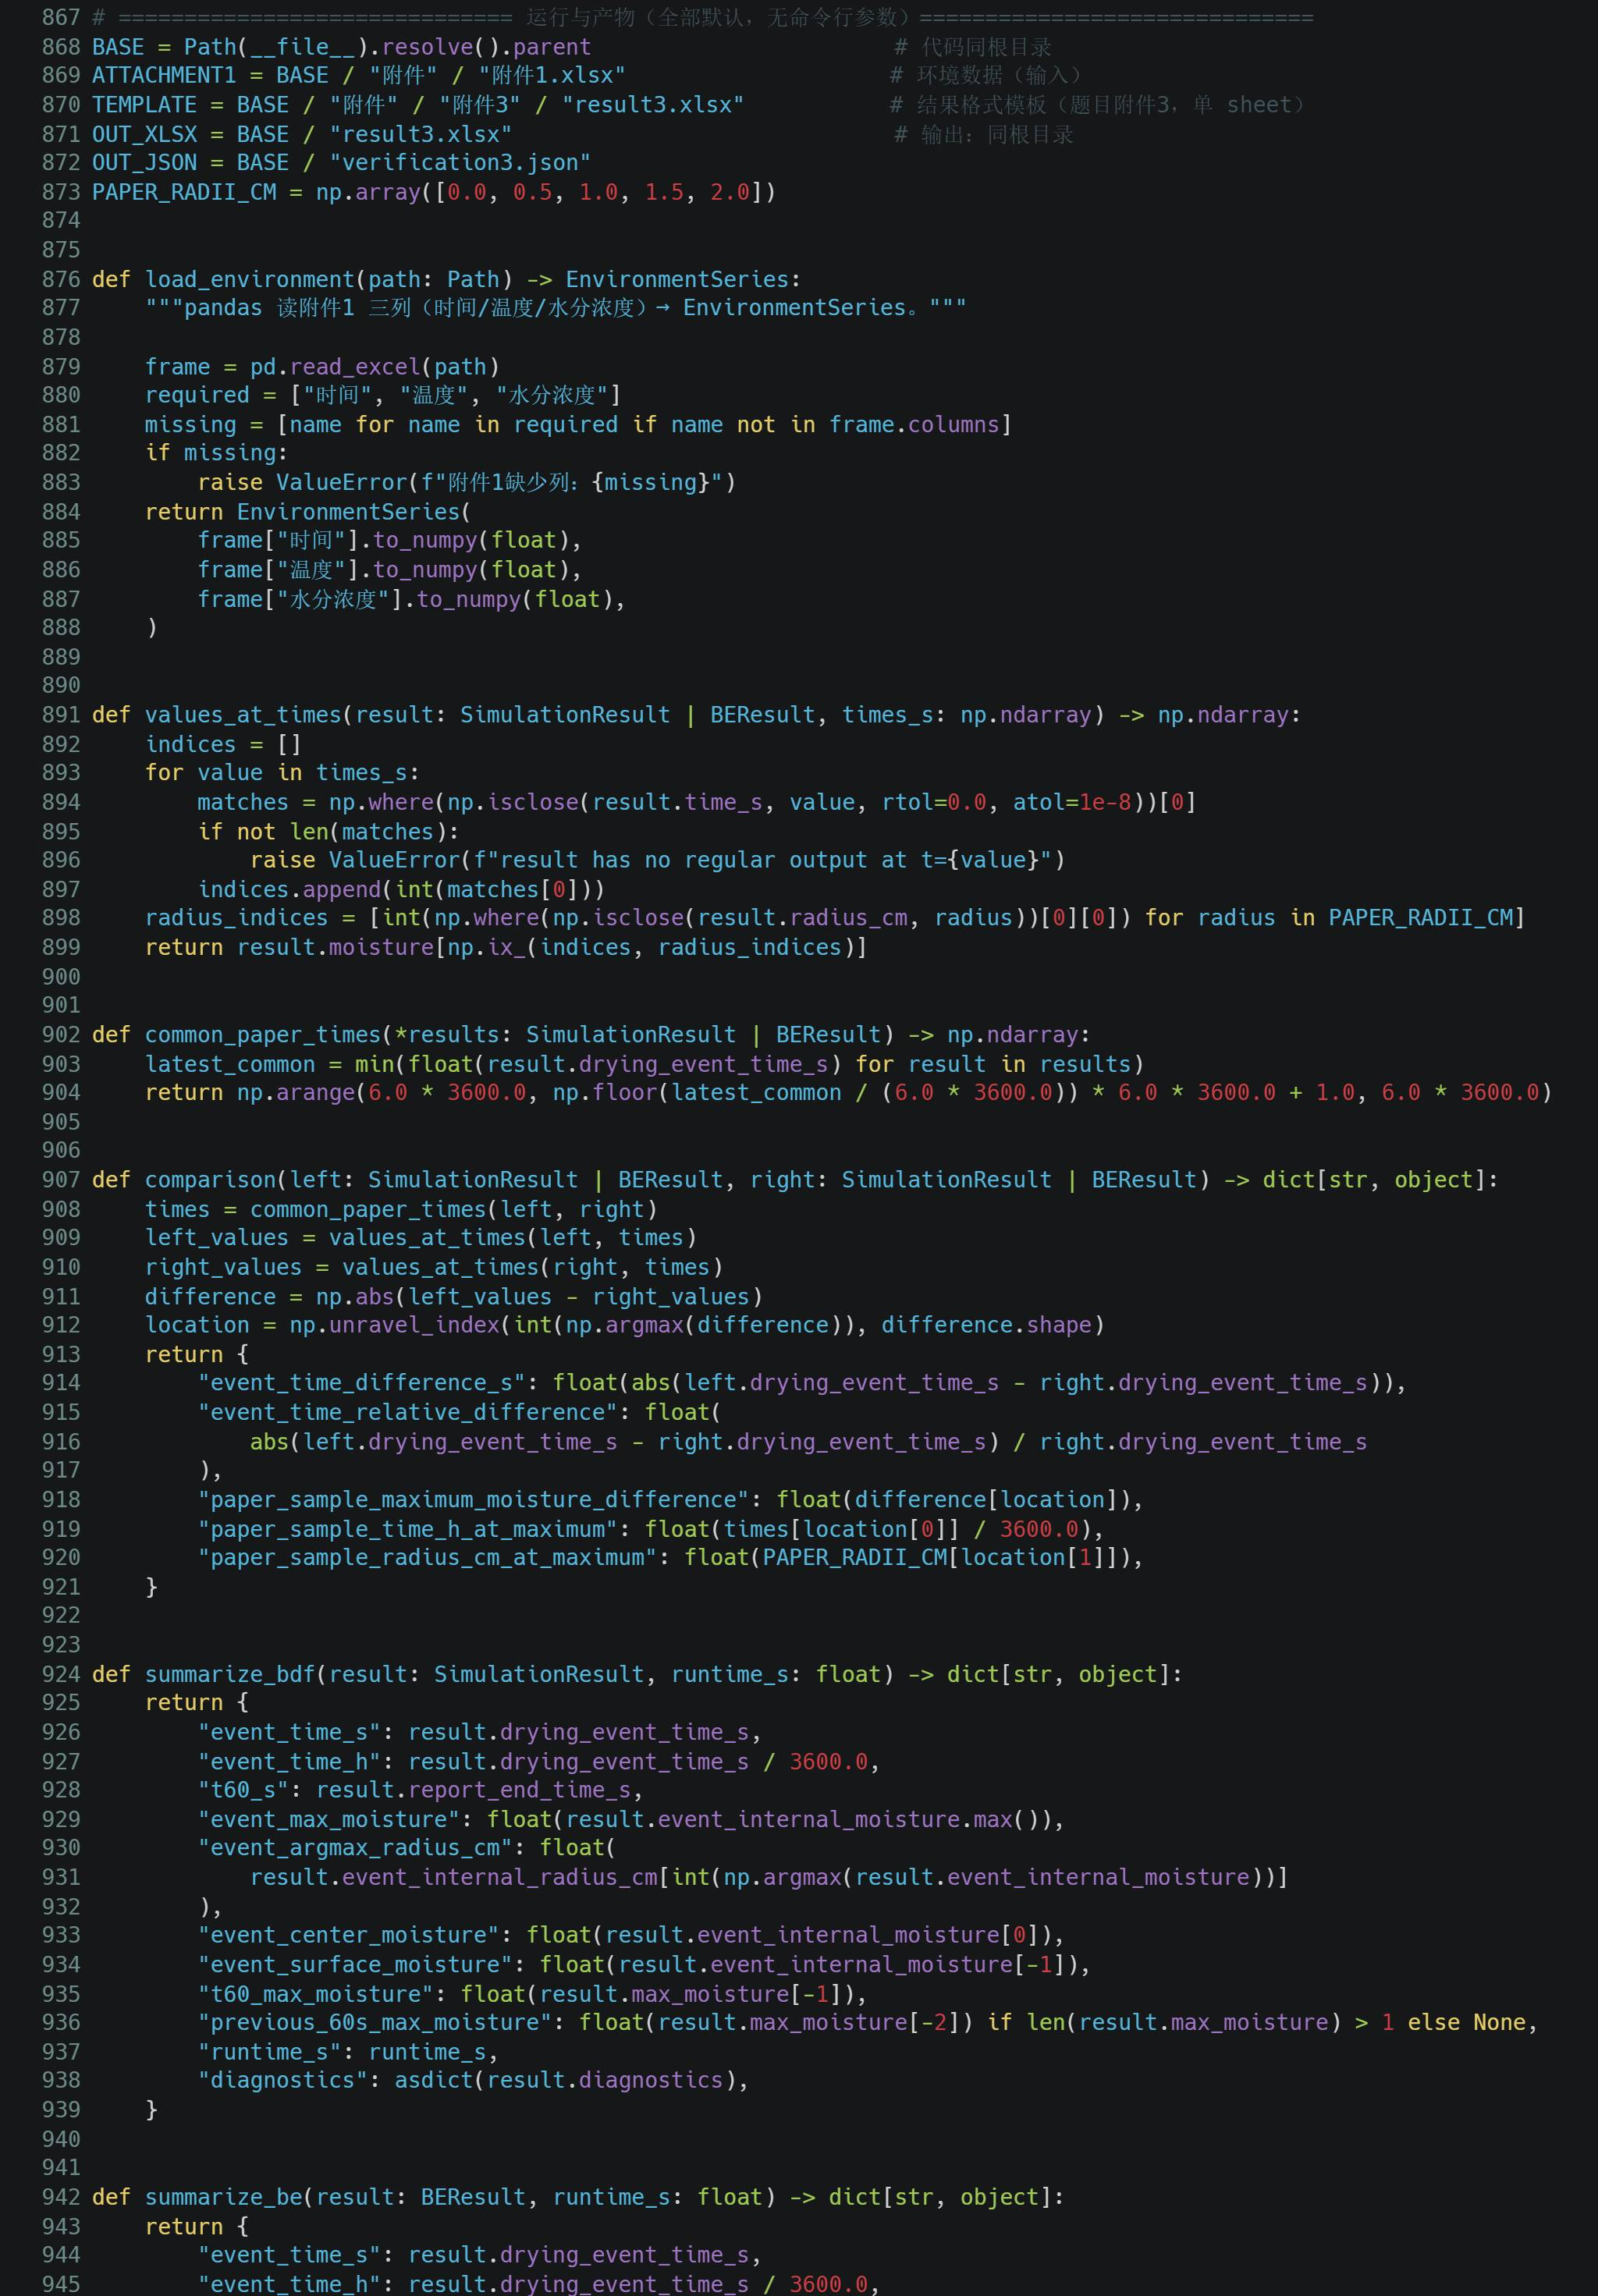
\includegraphics[width=\dimexpr\textwidth-24pt\relax]{../../code/submission/code_images/split/problem3_p12.jpg}
\newpage
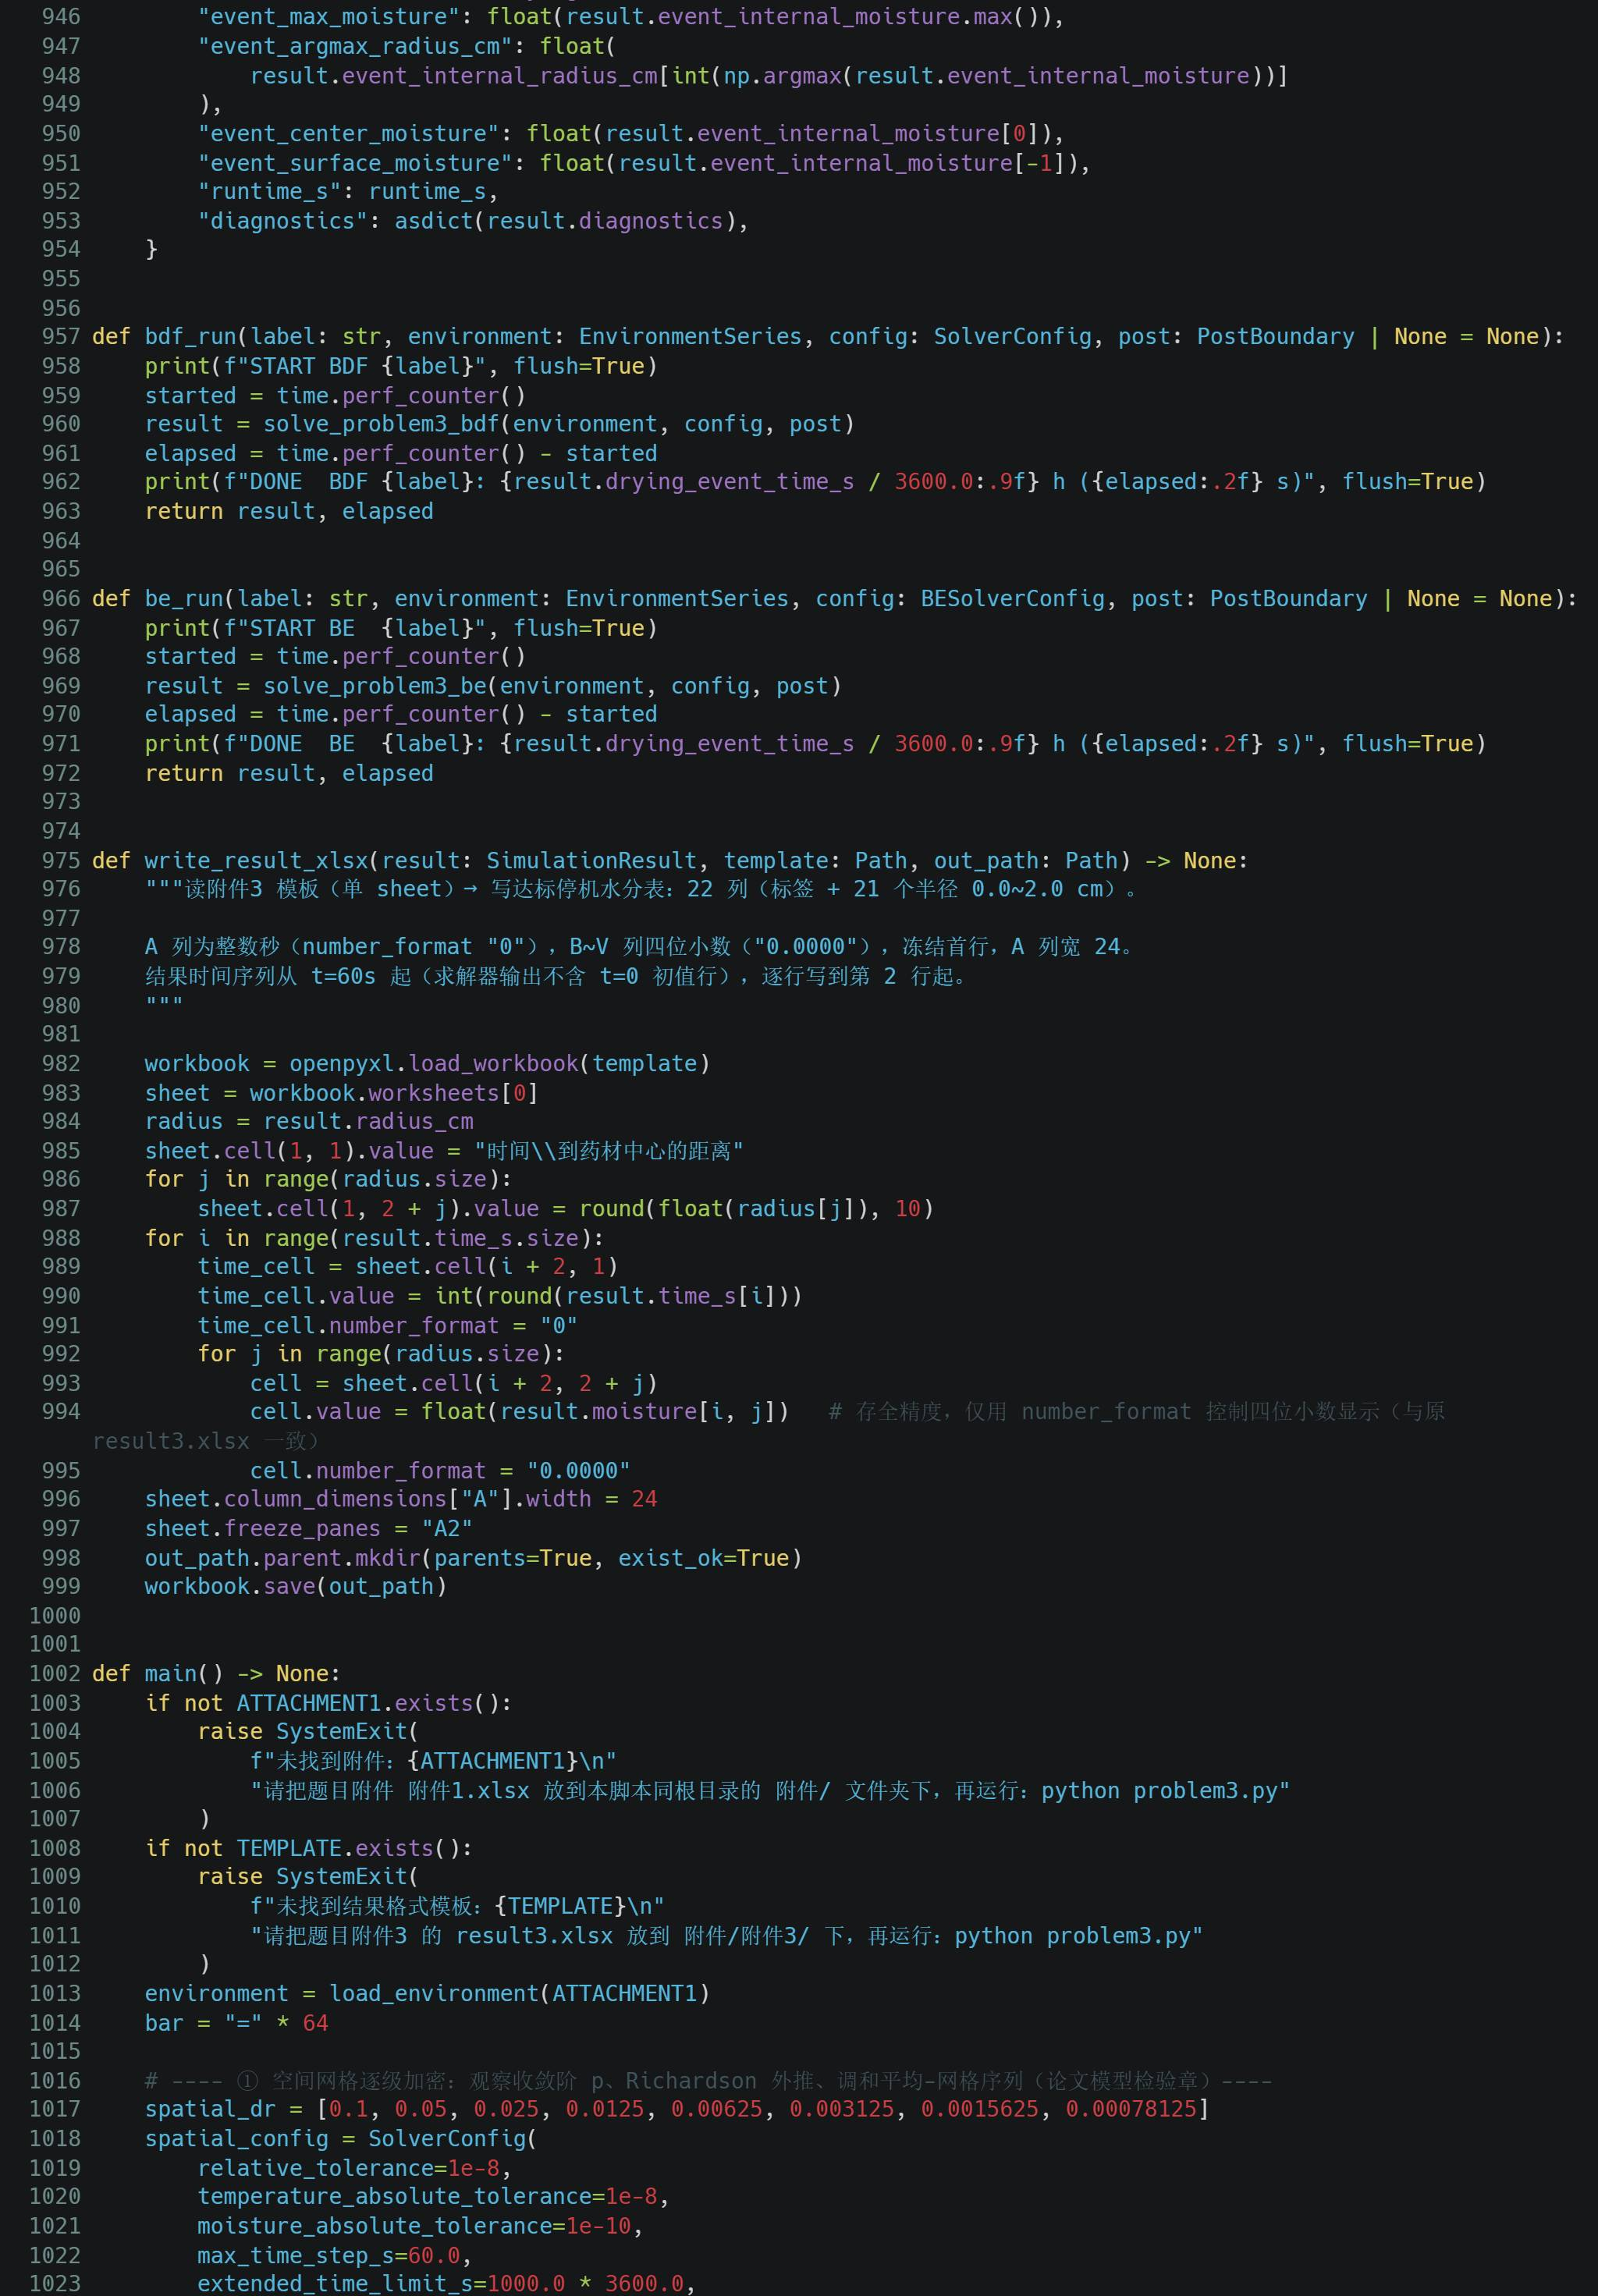
\includegraphics[width=\dimexpr\textwidth-24pt\relax]{../../code/submission/code_images/split/problem3_p13.jpg}
\newpage
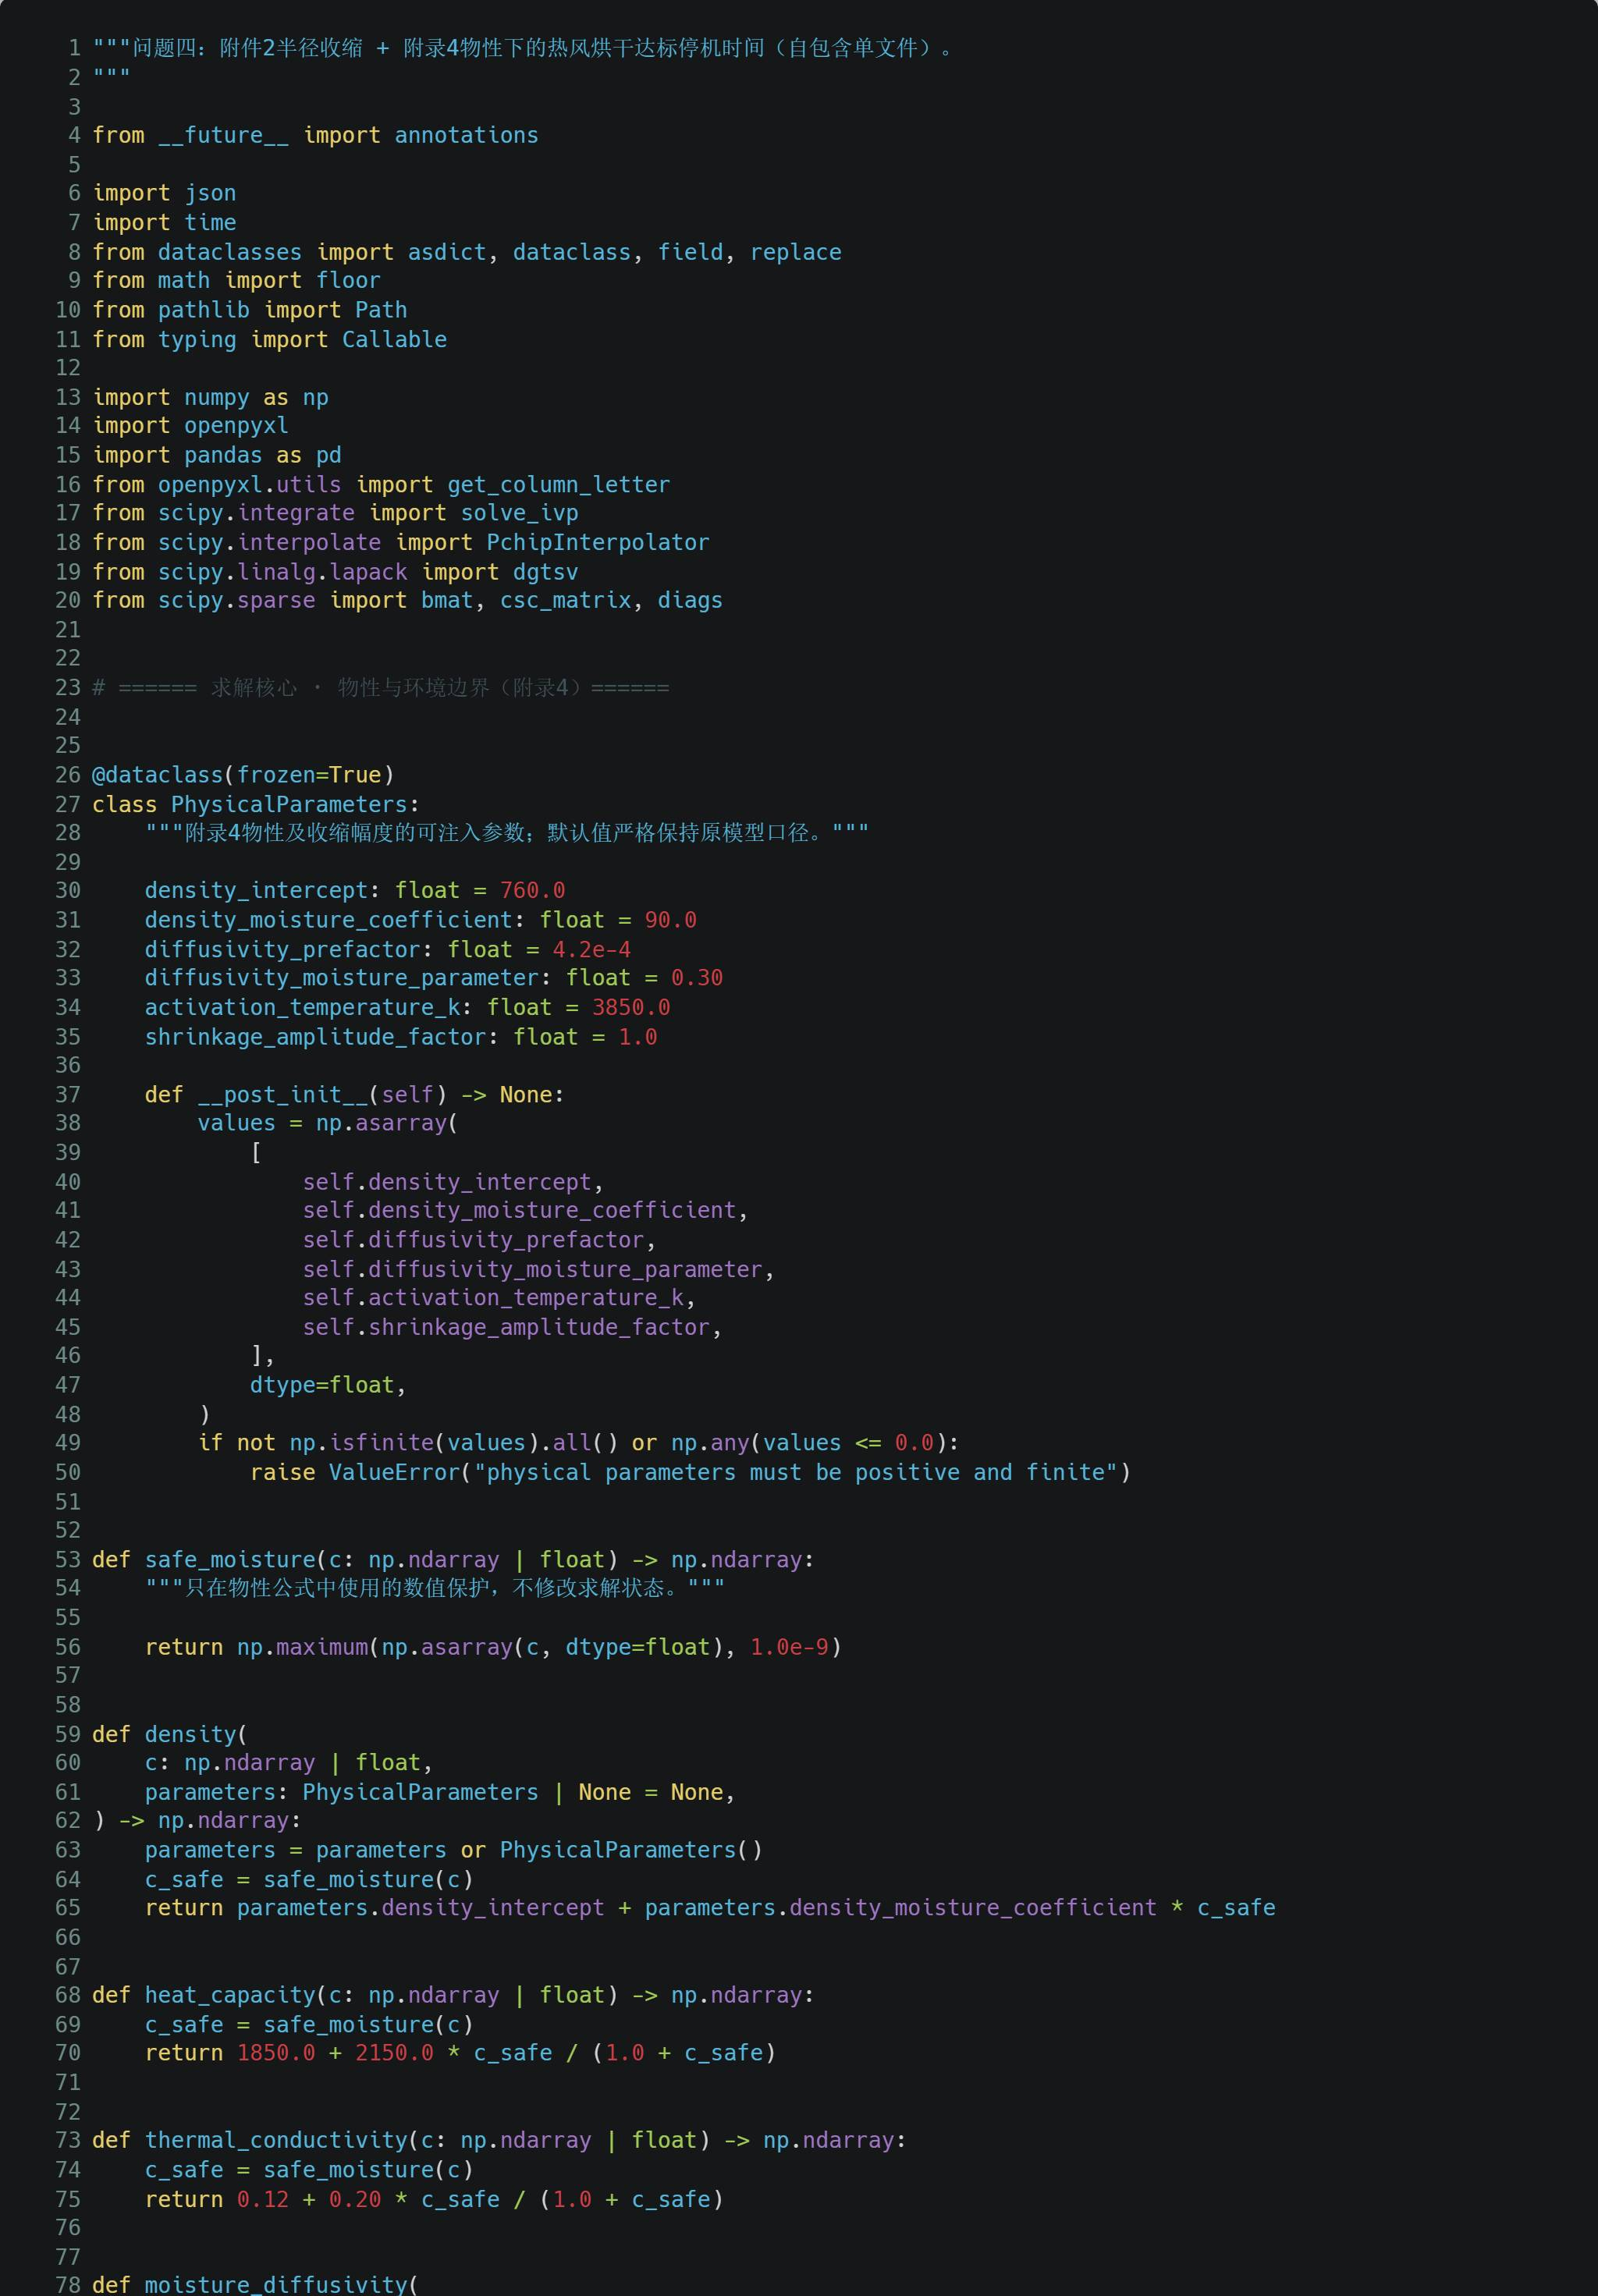
\includegraphics[width=\dimexpr\textwidth-24pt\relax]{../../code/submission/code_images/split/problem4_p1.jpg}
\newpage
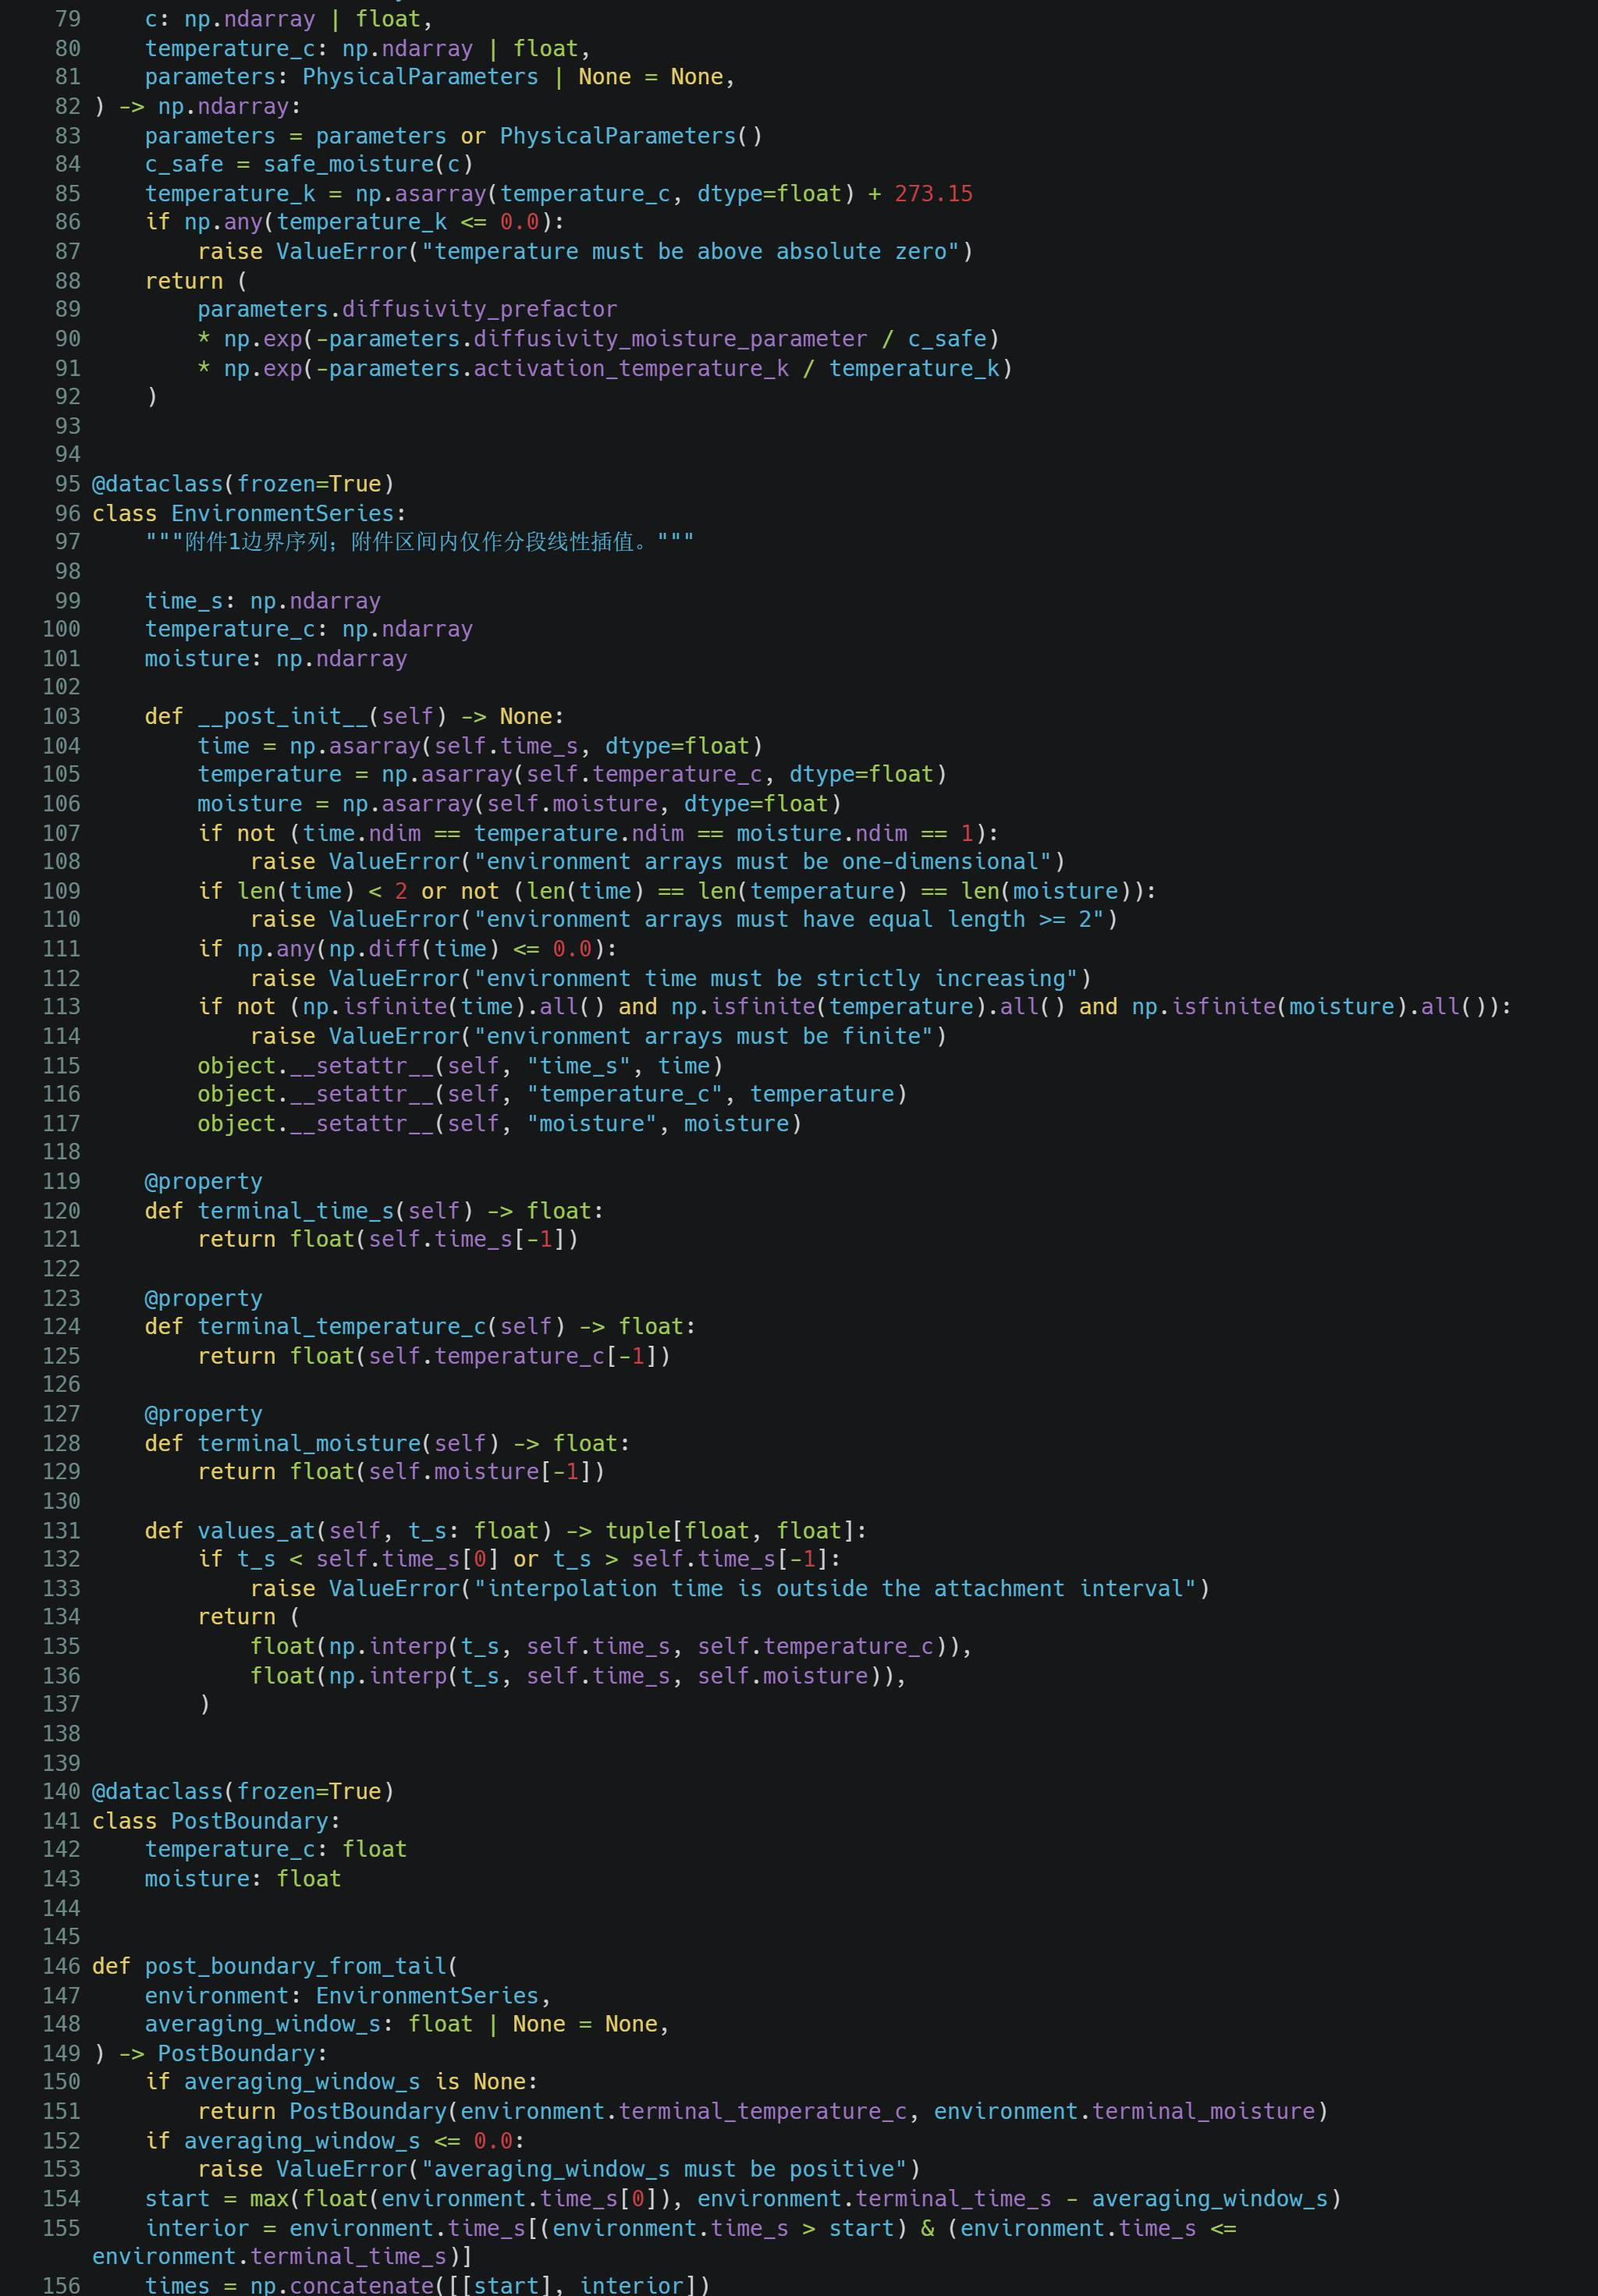
\includegraphics[width=\dimexpr\textwidth-24pt\relax]{../../code/submission/code_images/split/problem4_p2.jpg}
\newpage
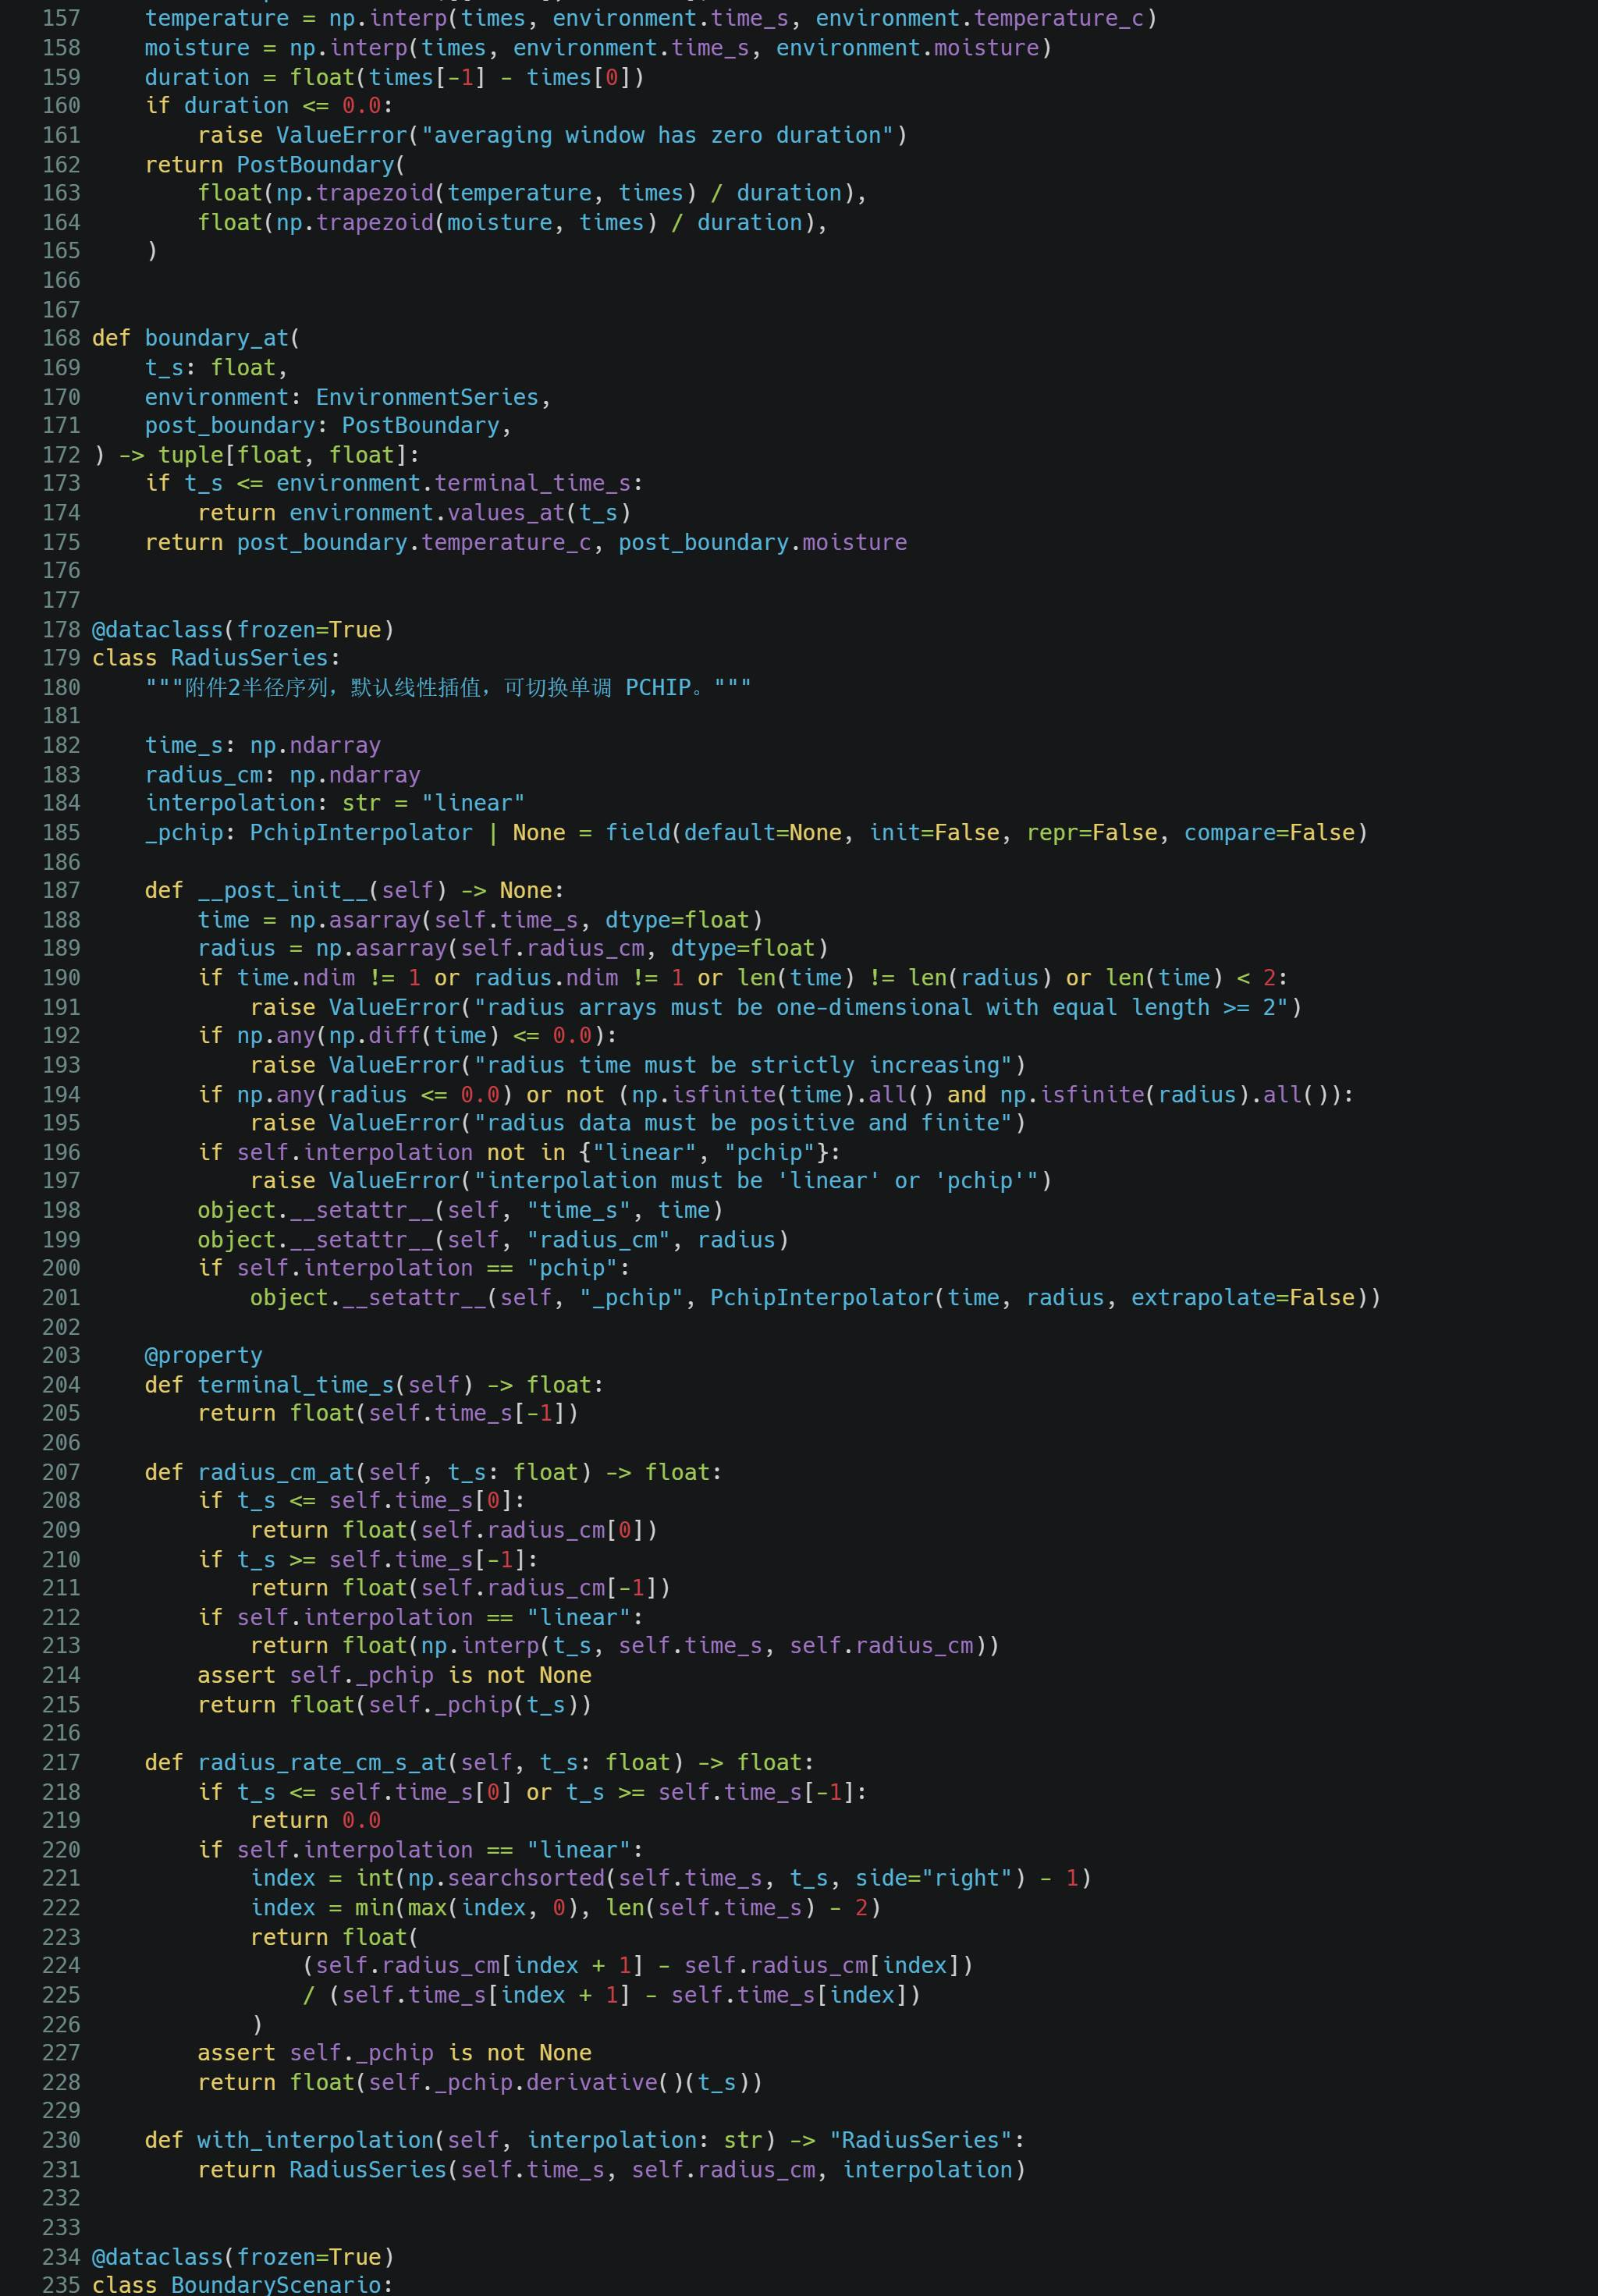
\includegraphics[width=\dimexpr\textwidth-24pt\relax]{../../code/submission/code_images/split/problem4_p3.jpg}
\newpage
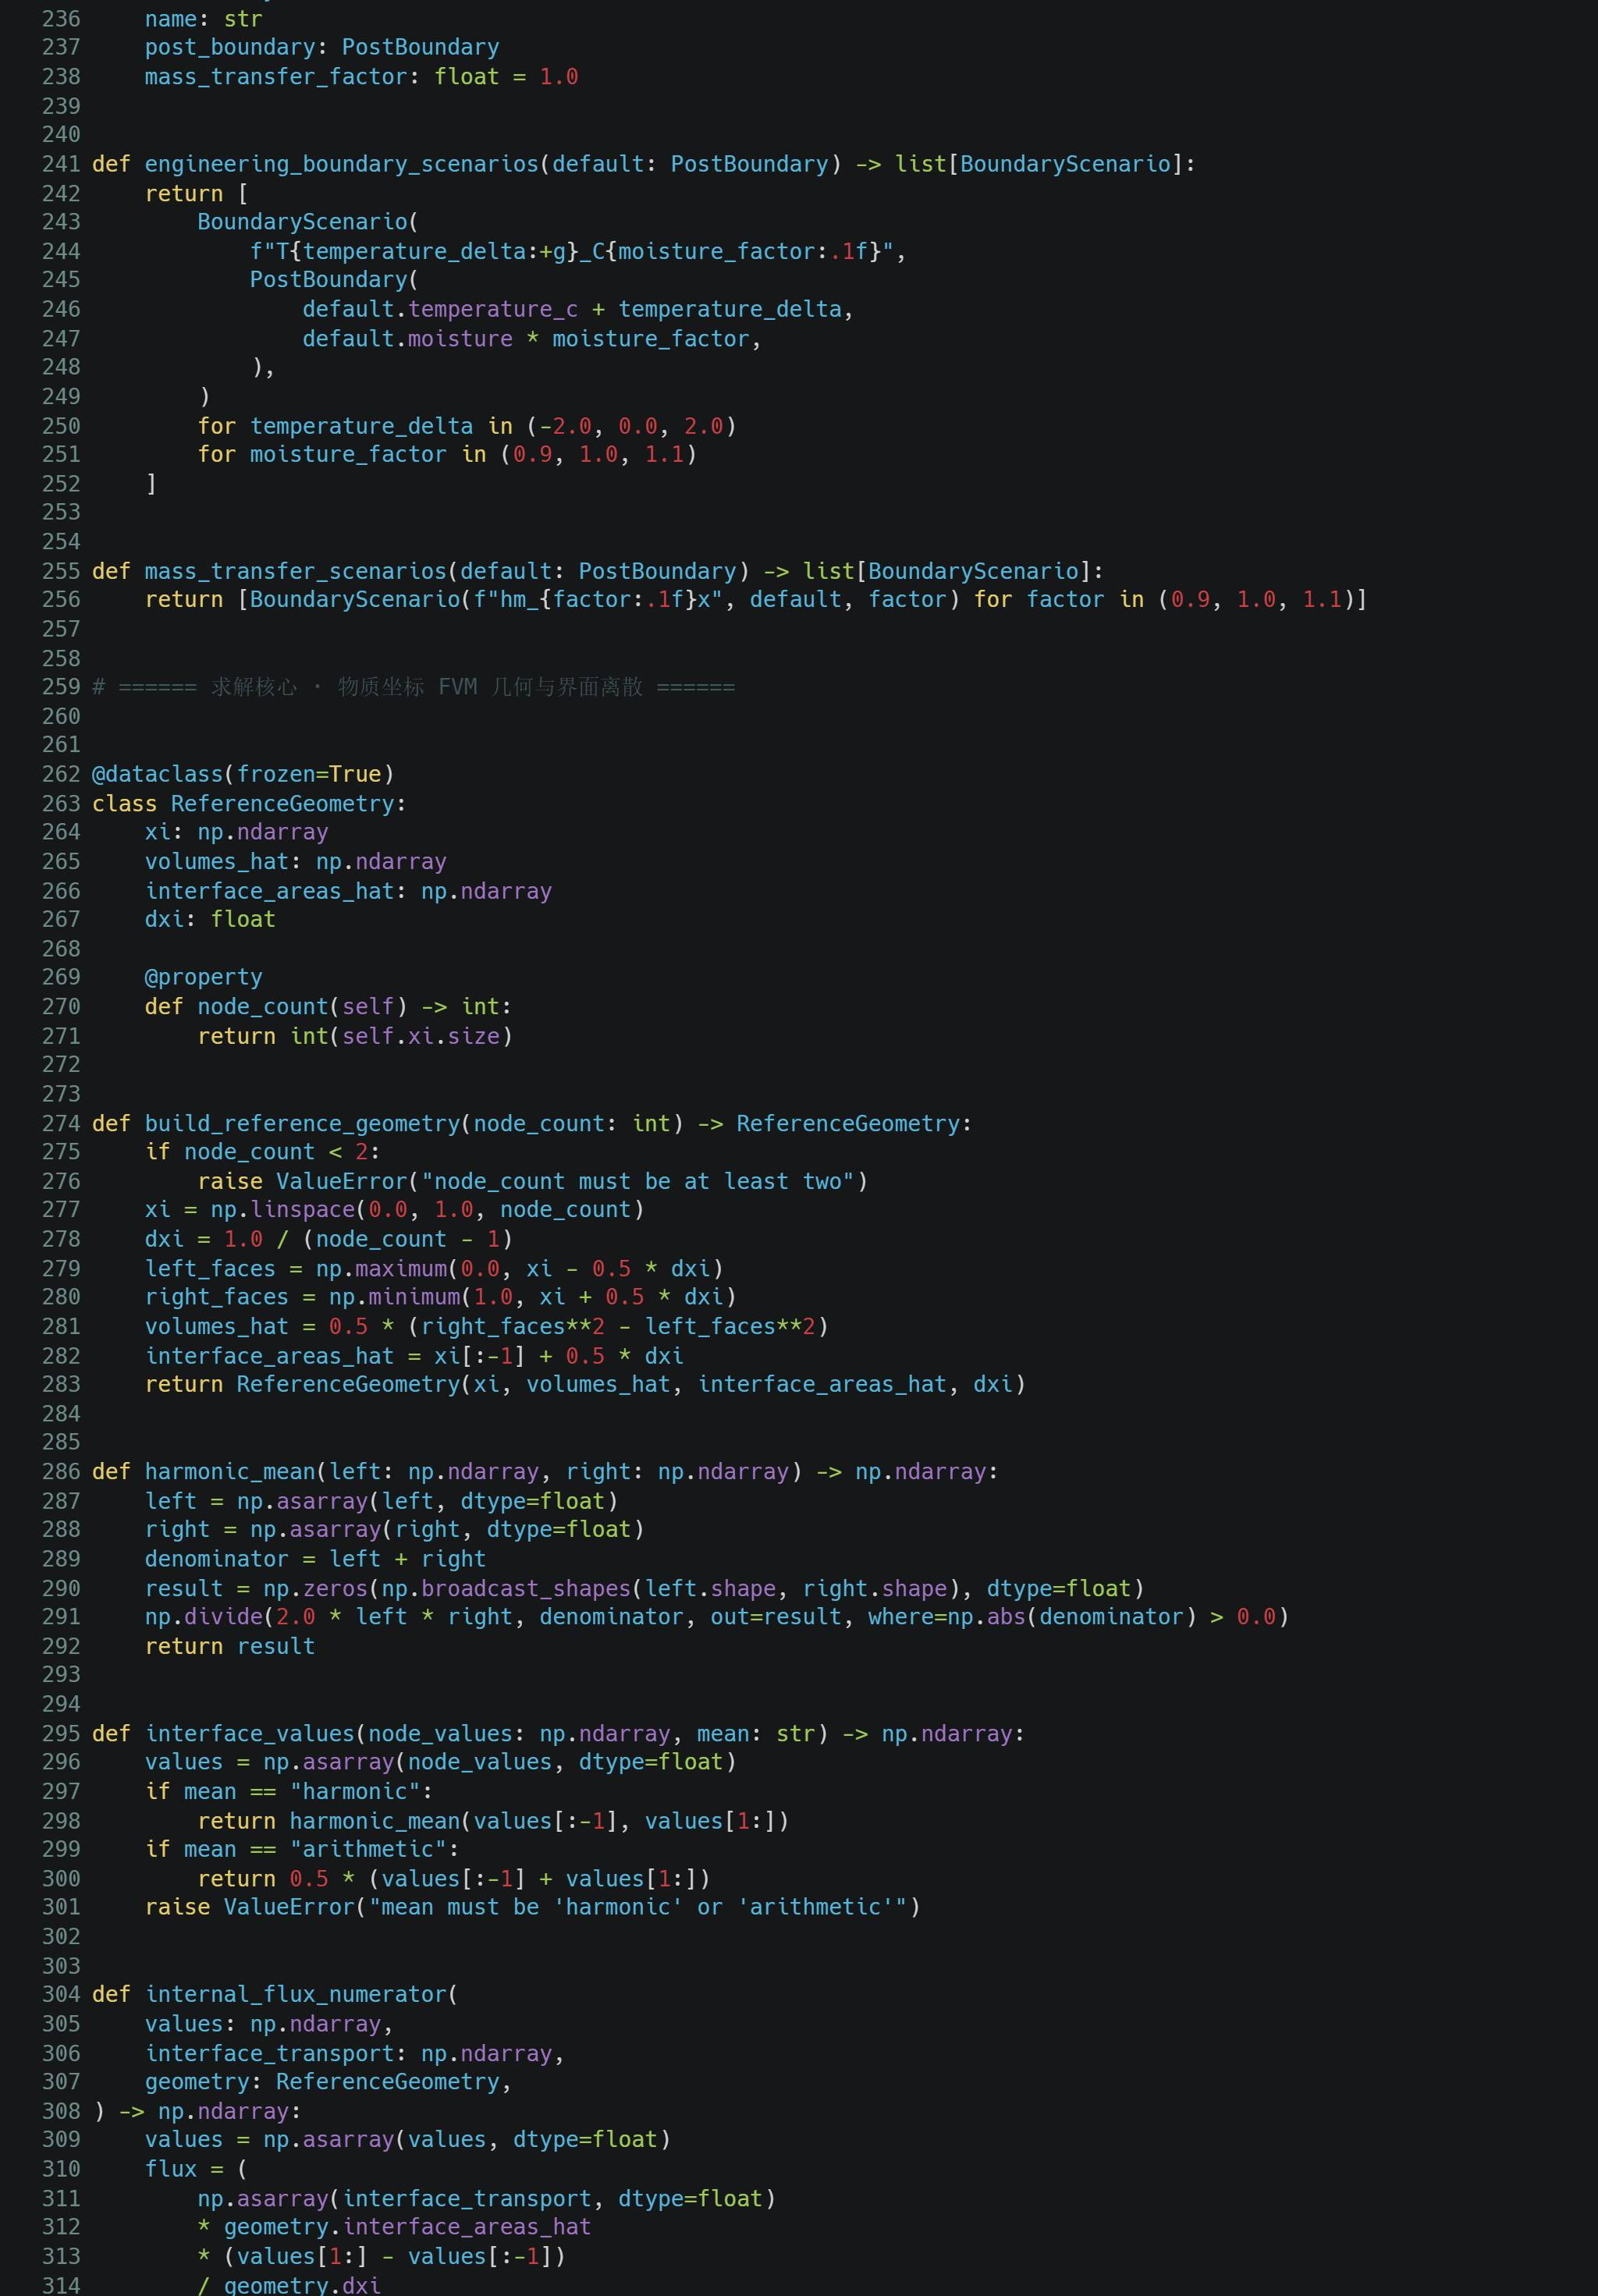
\includegraphics[width=\dimexpr\textwidth-24pt\relax]{../../code/submission/code_images/split/problem4_p4.jpg}
\newpage
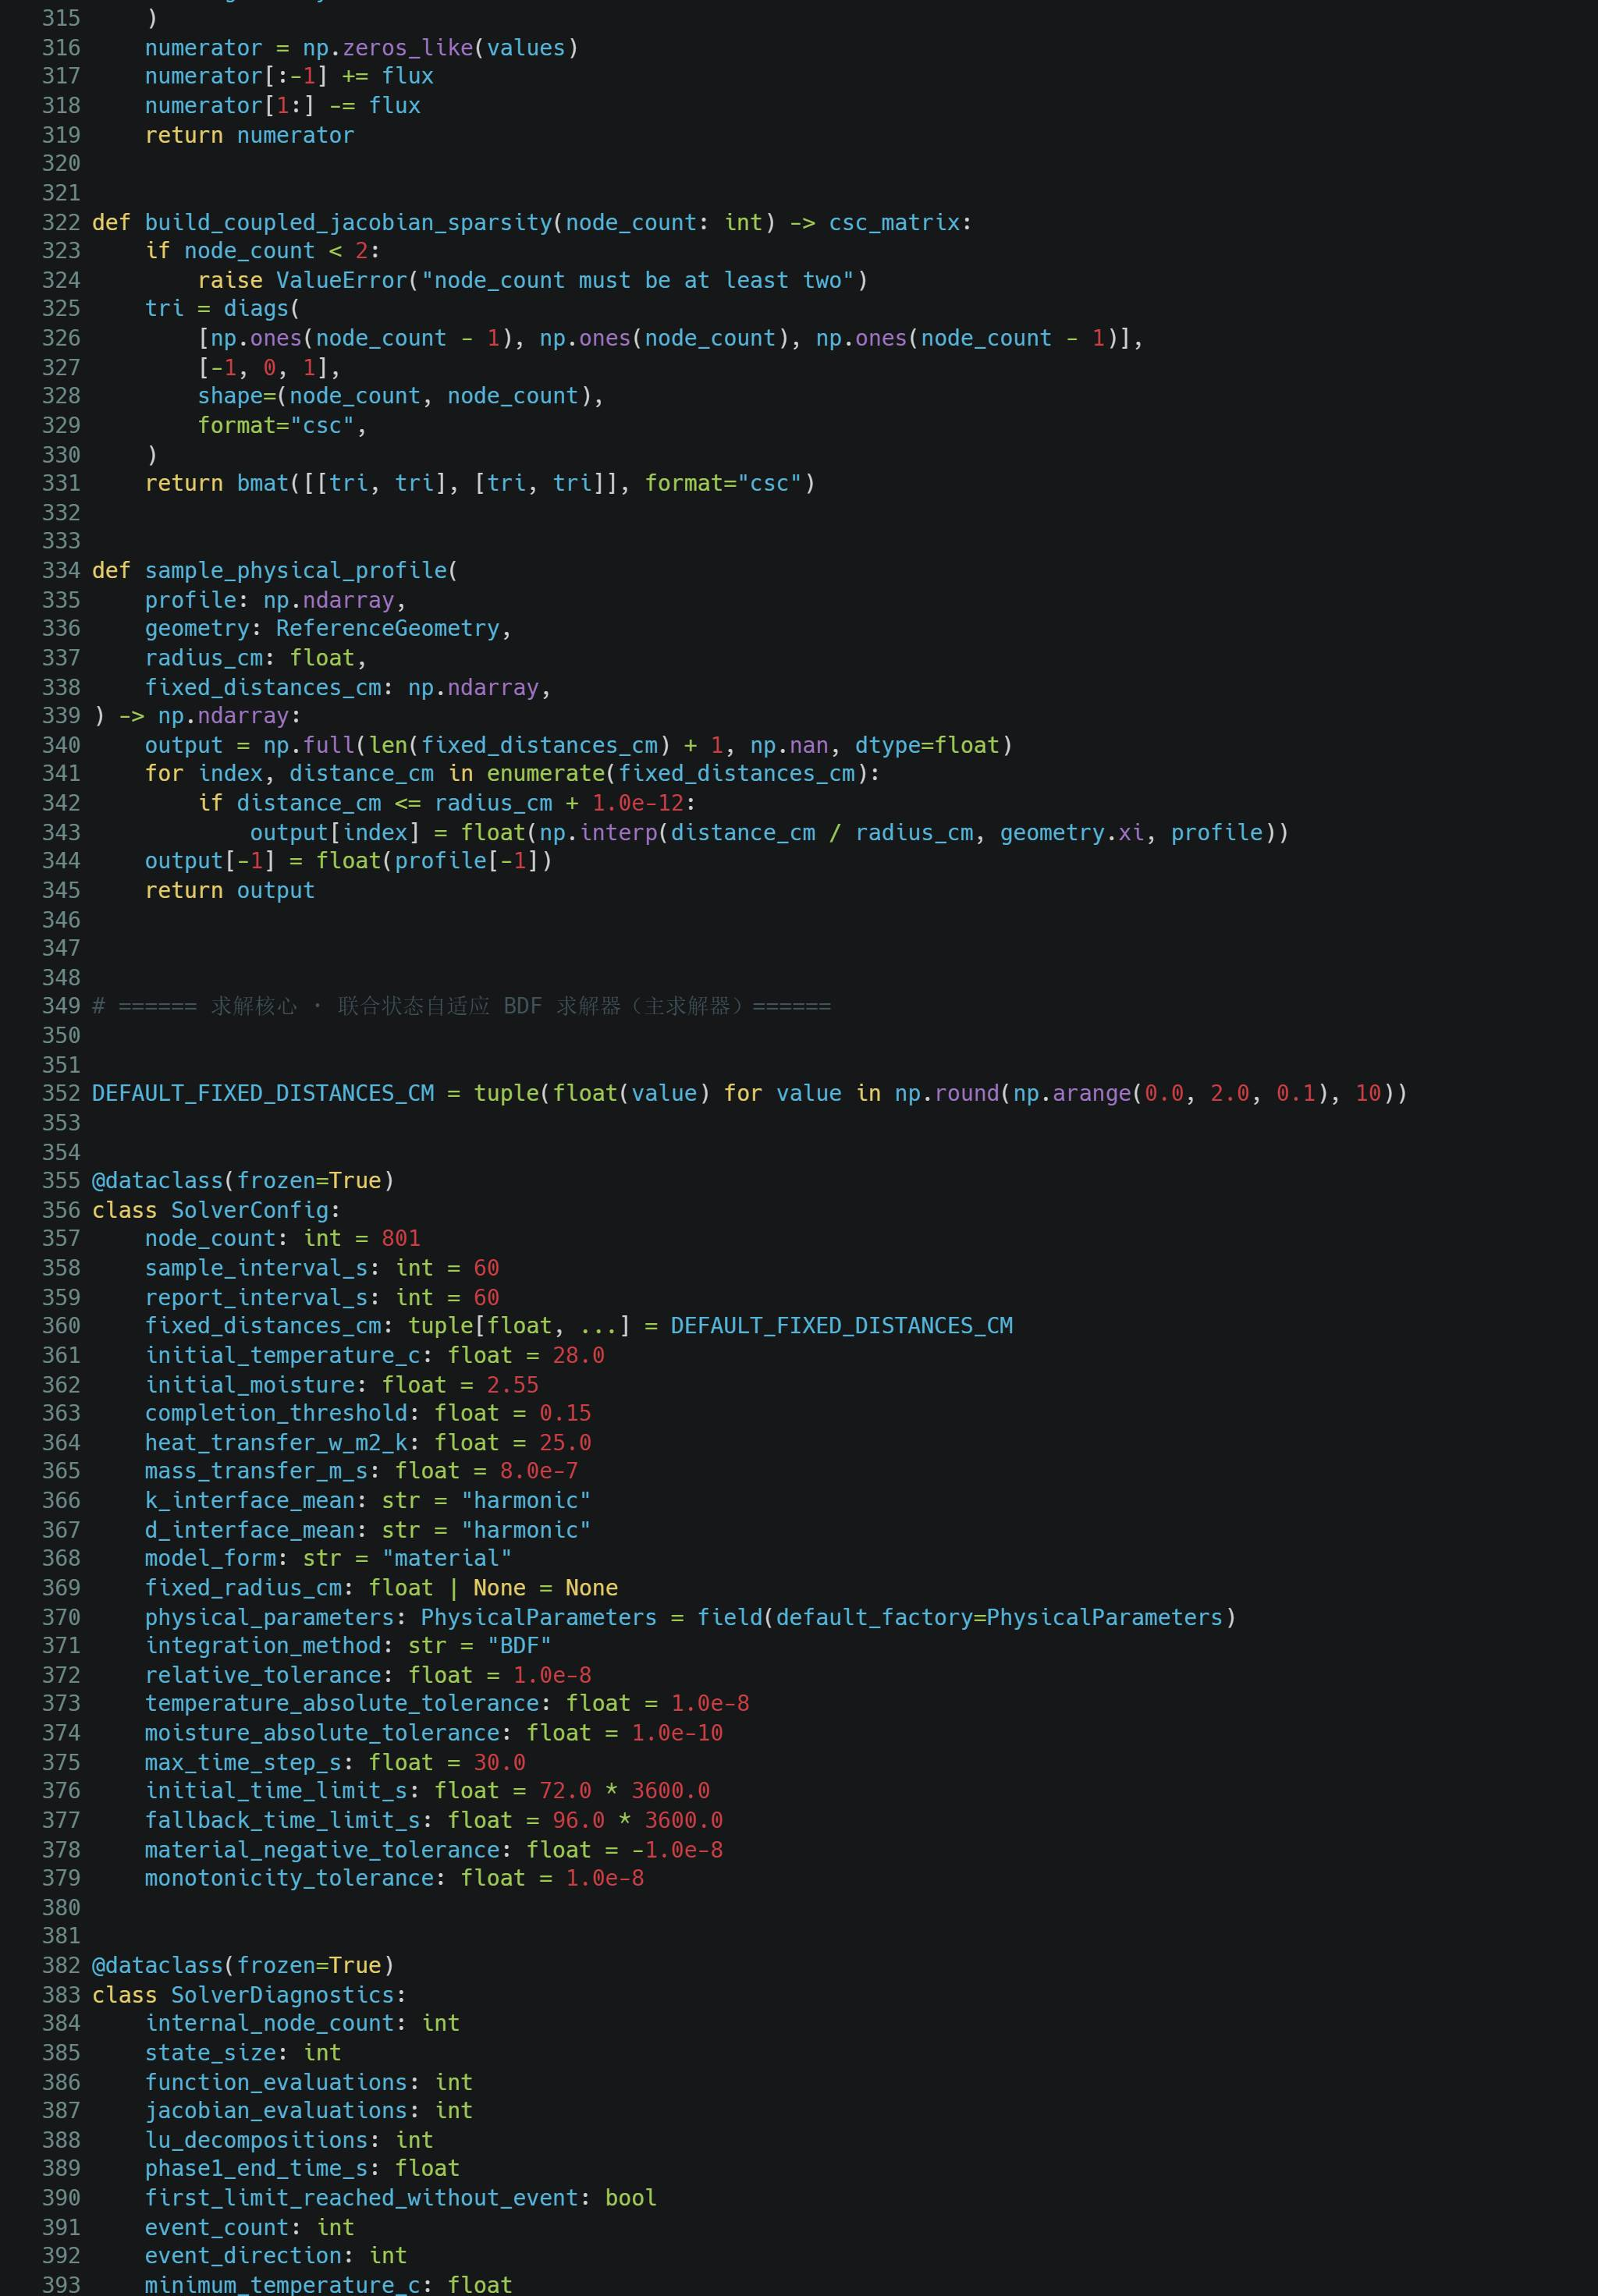
\includegraphics[width=\dimexpr\textwidth-24pt\relax]{../../code/submission/code_images/split/problem4_p5.jpg}
\newpage
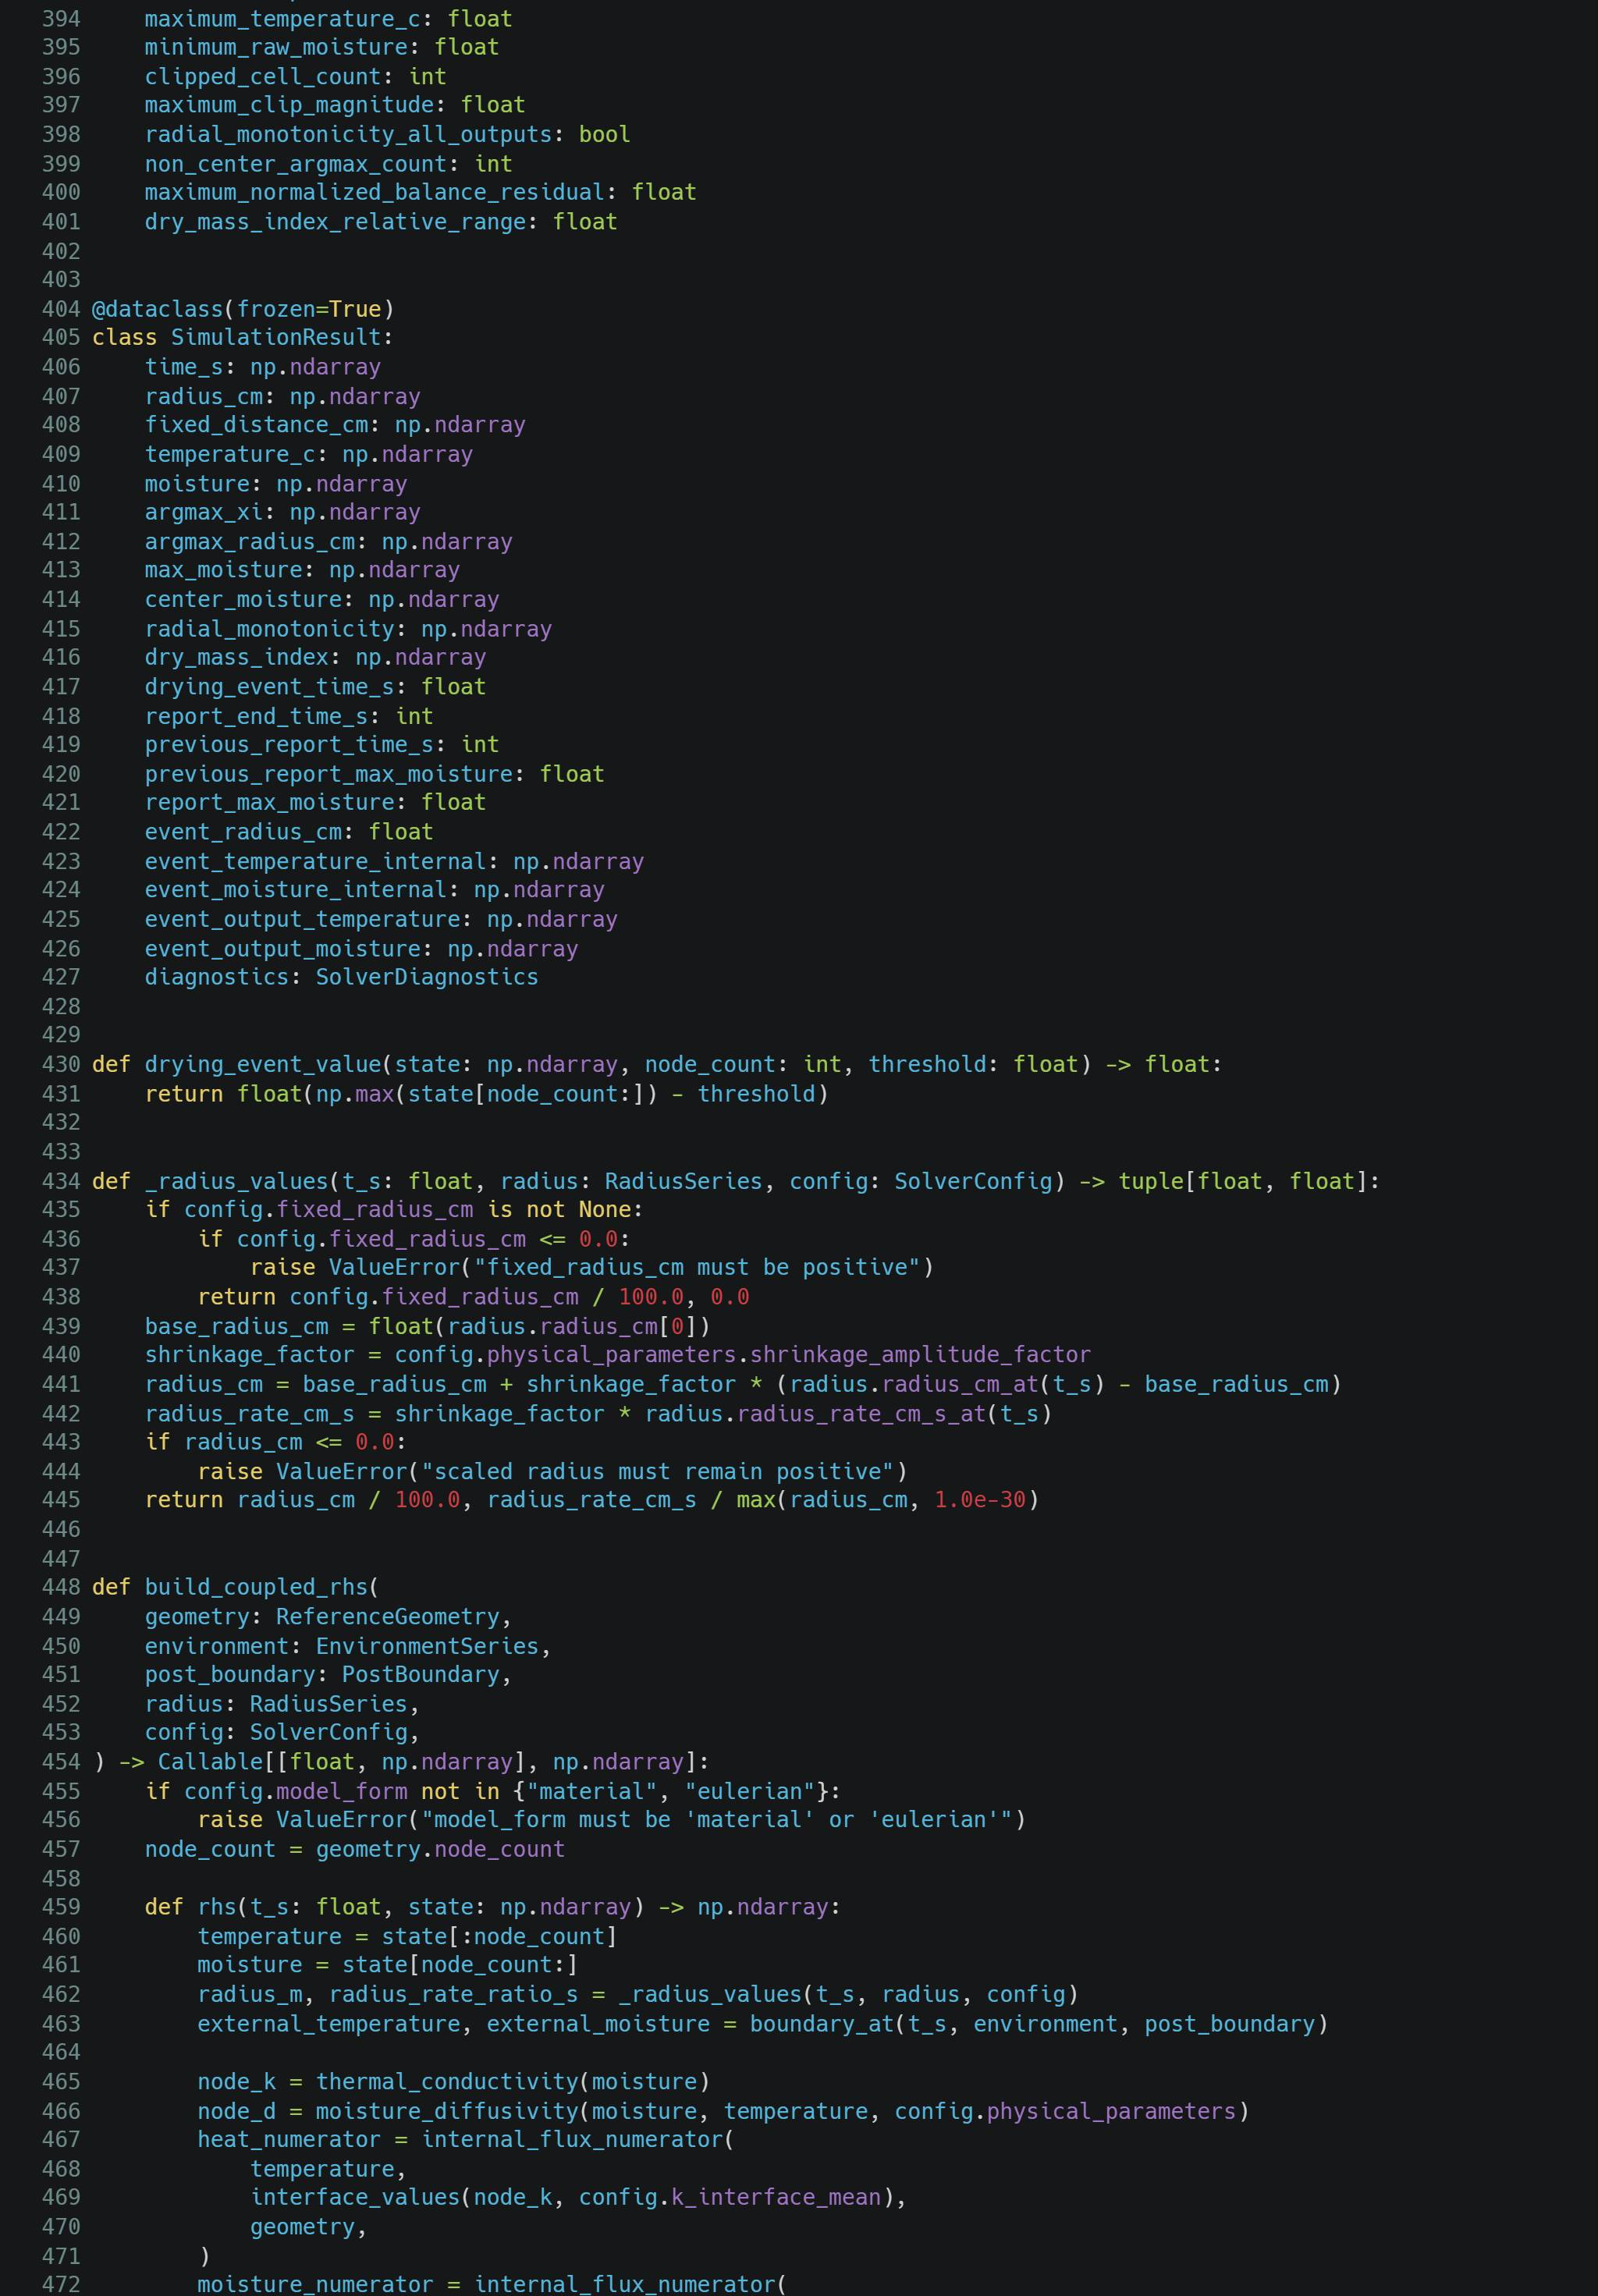
\includegraphics[width=\dimexpr\textwidth-24pt\relax]{../../code/submission/code_images/split/problem4_p6.jpg}
\newpage
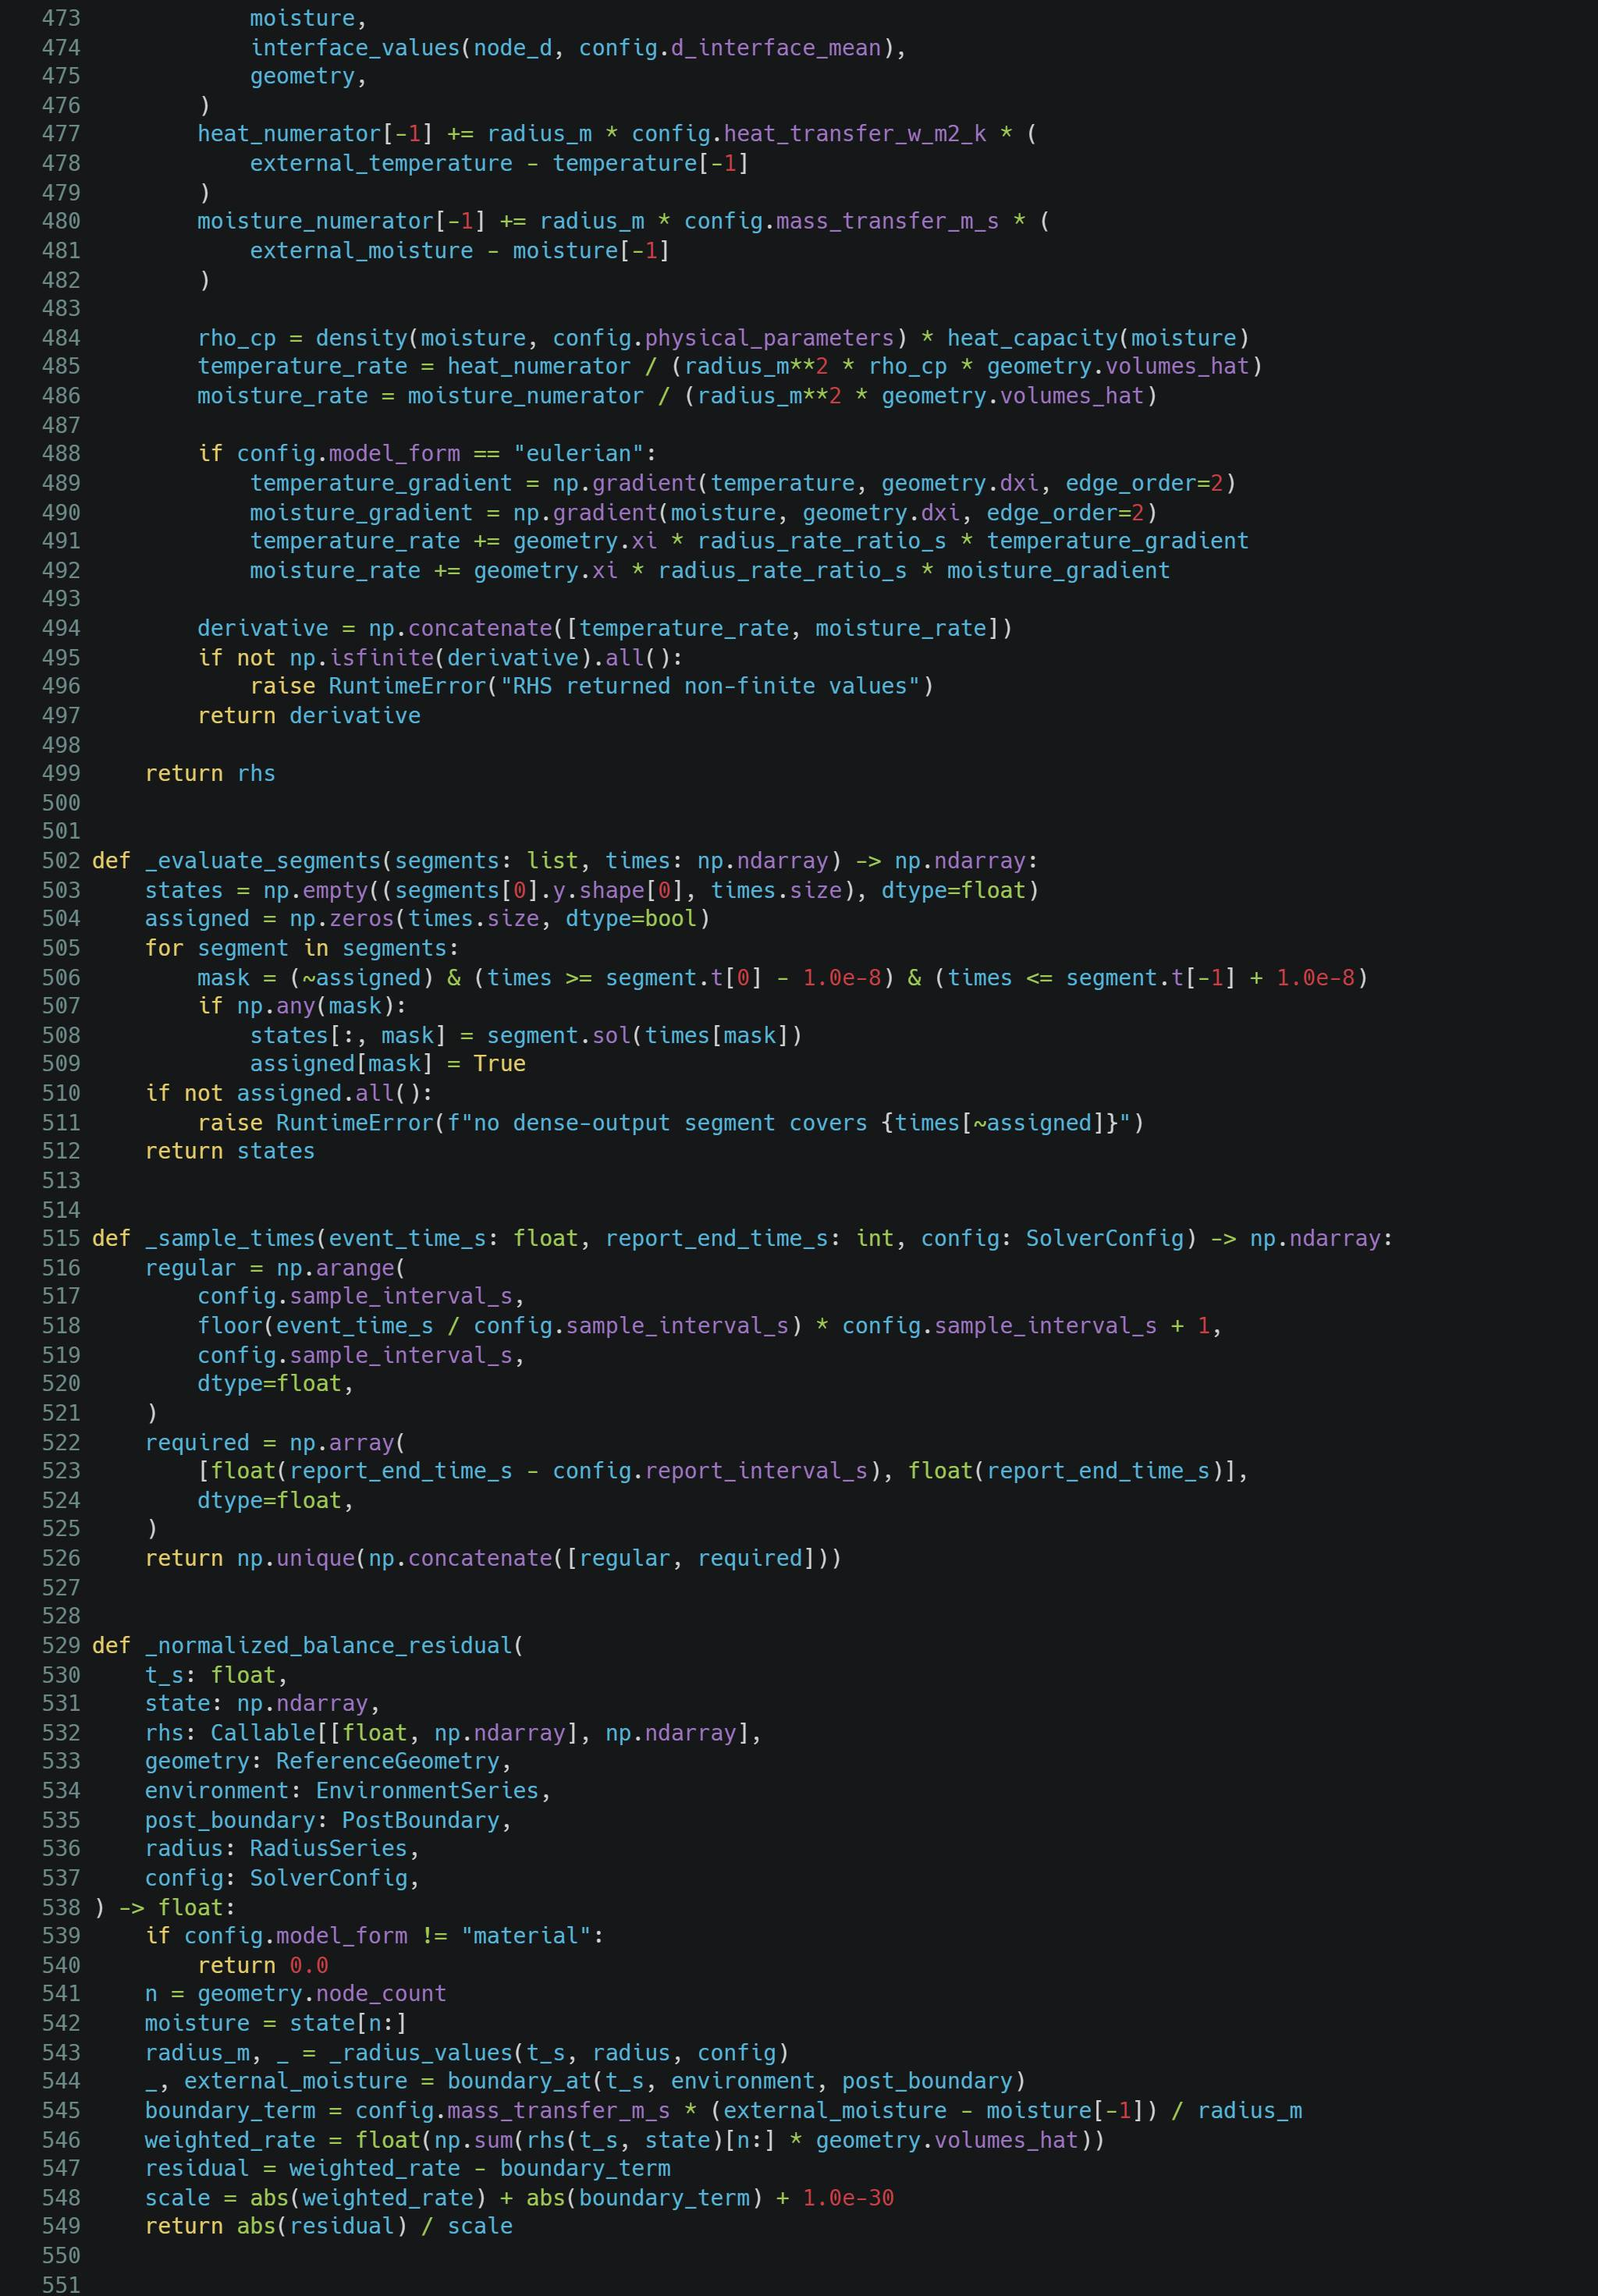
\includegraphics[width=\dimexpr\textwidth-24pt\relax]{../../code/submission/code_images/split/problem4_p7.jpg}
\newpage
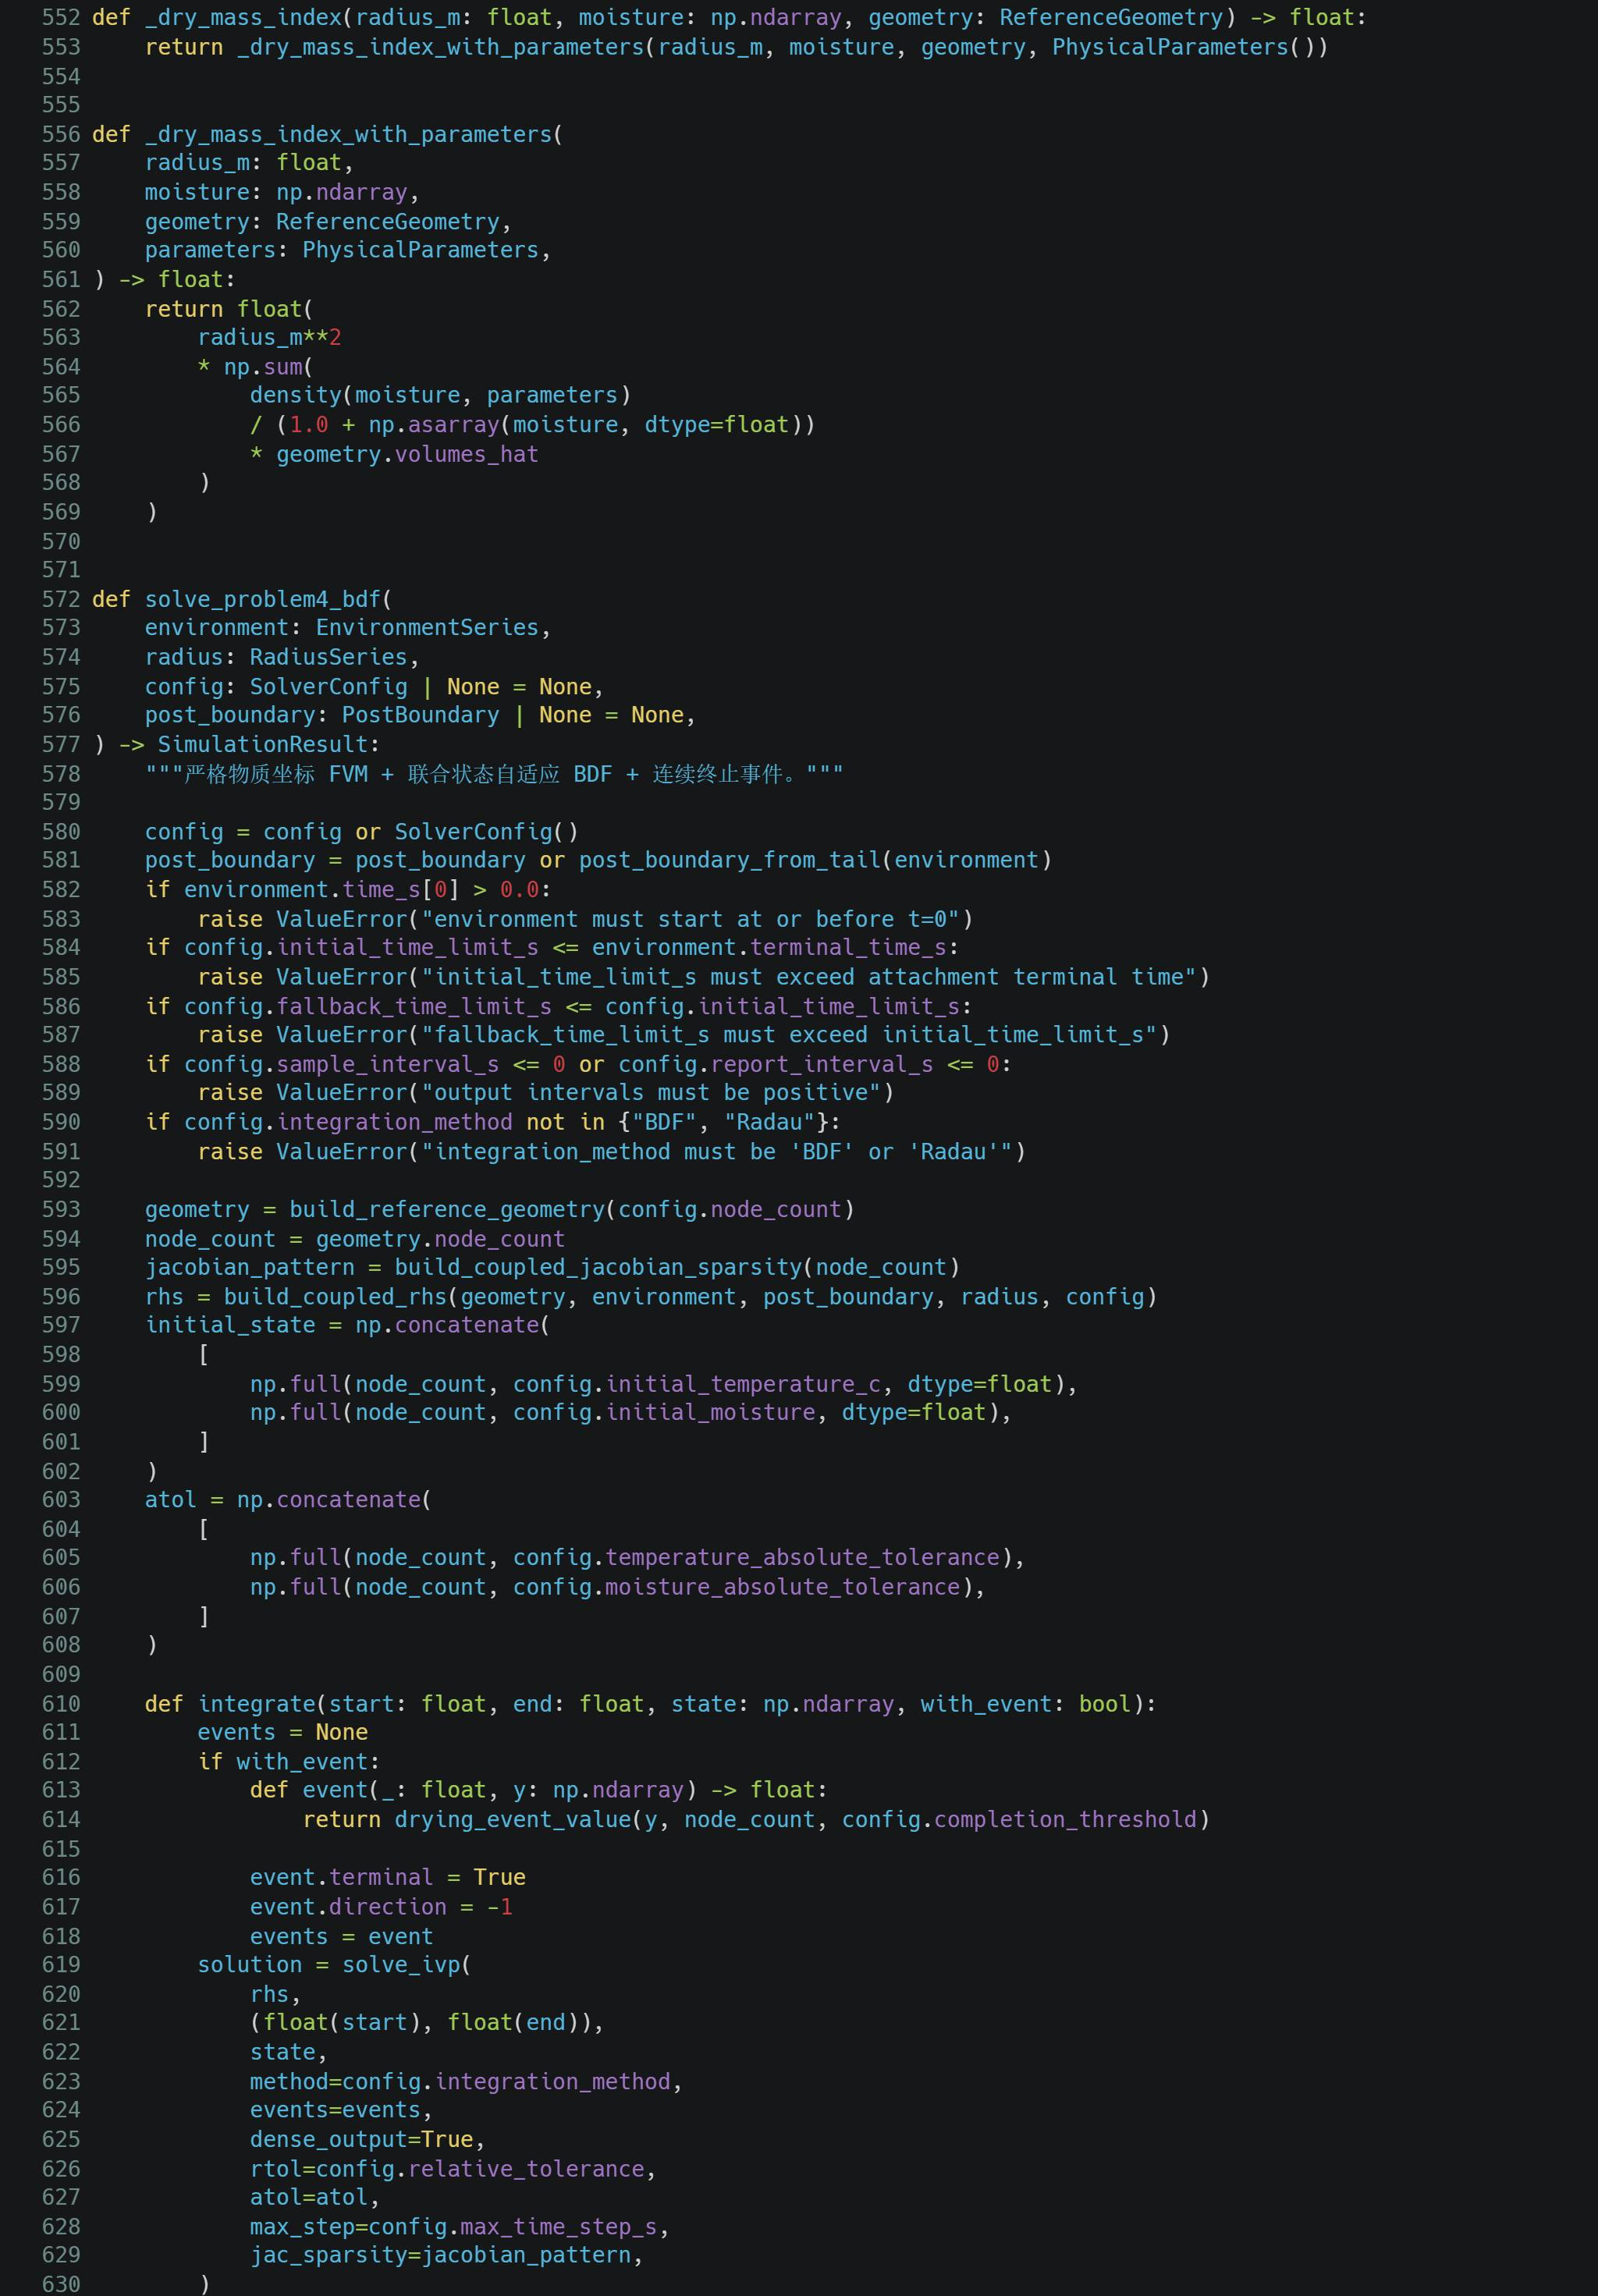
\includegraphics[width=\dimexpr\textwidth-24pt\relax]{../../code/submission/code_images/split/problem4_p8.jpg}
\newpage
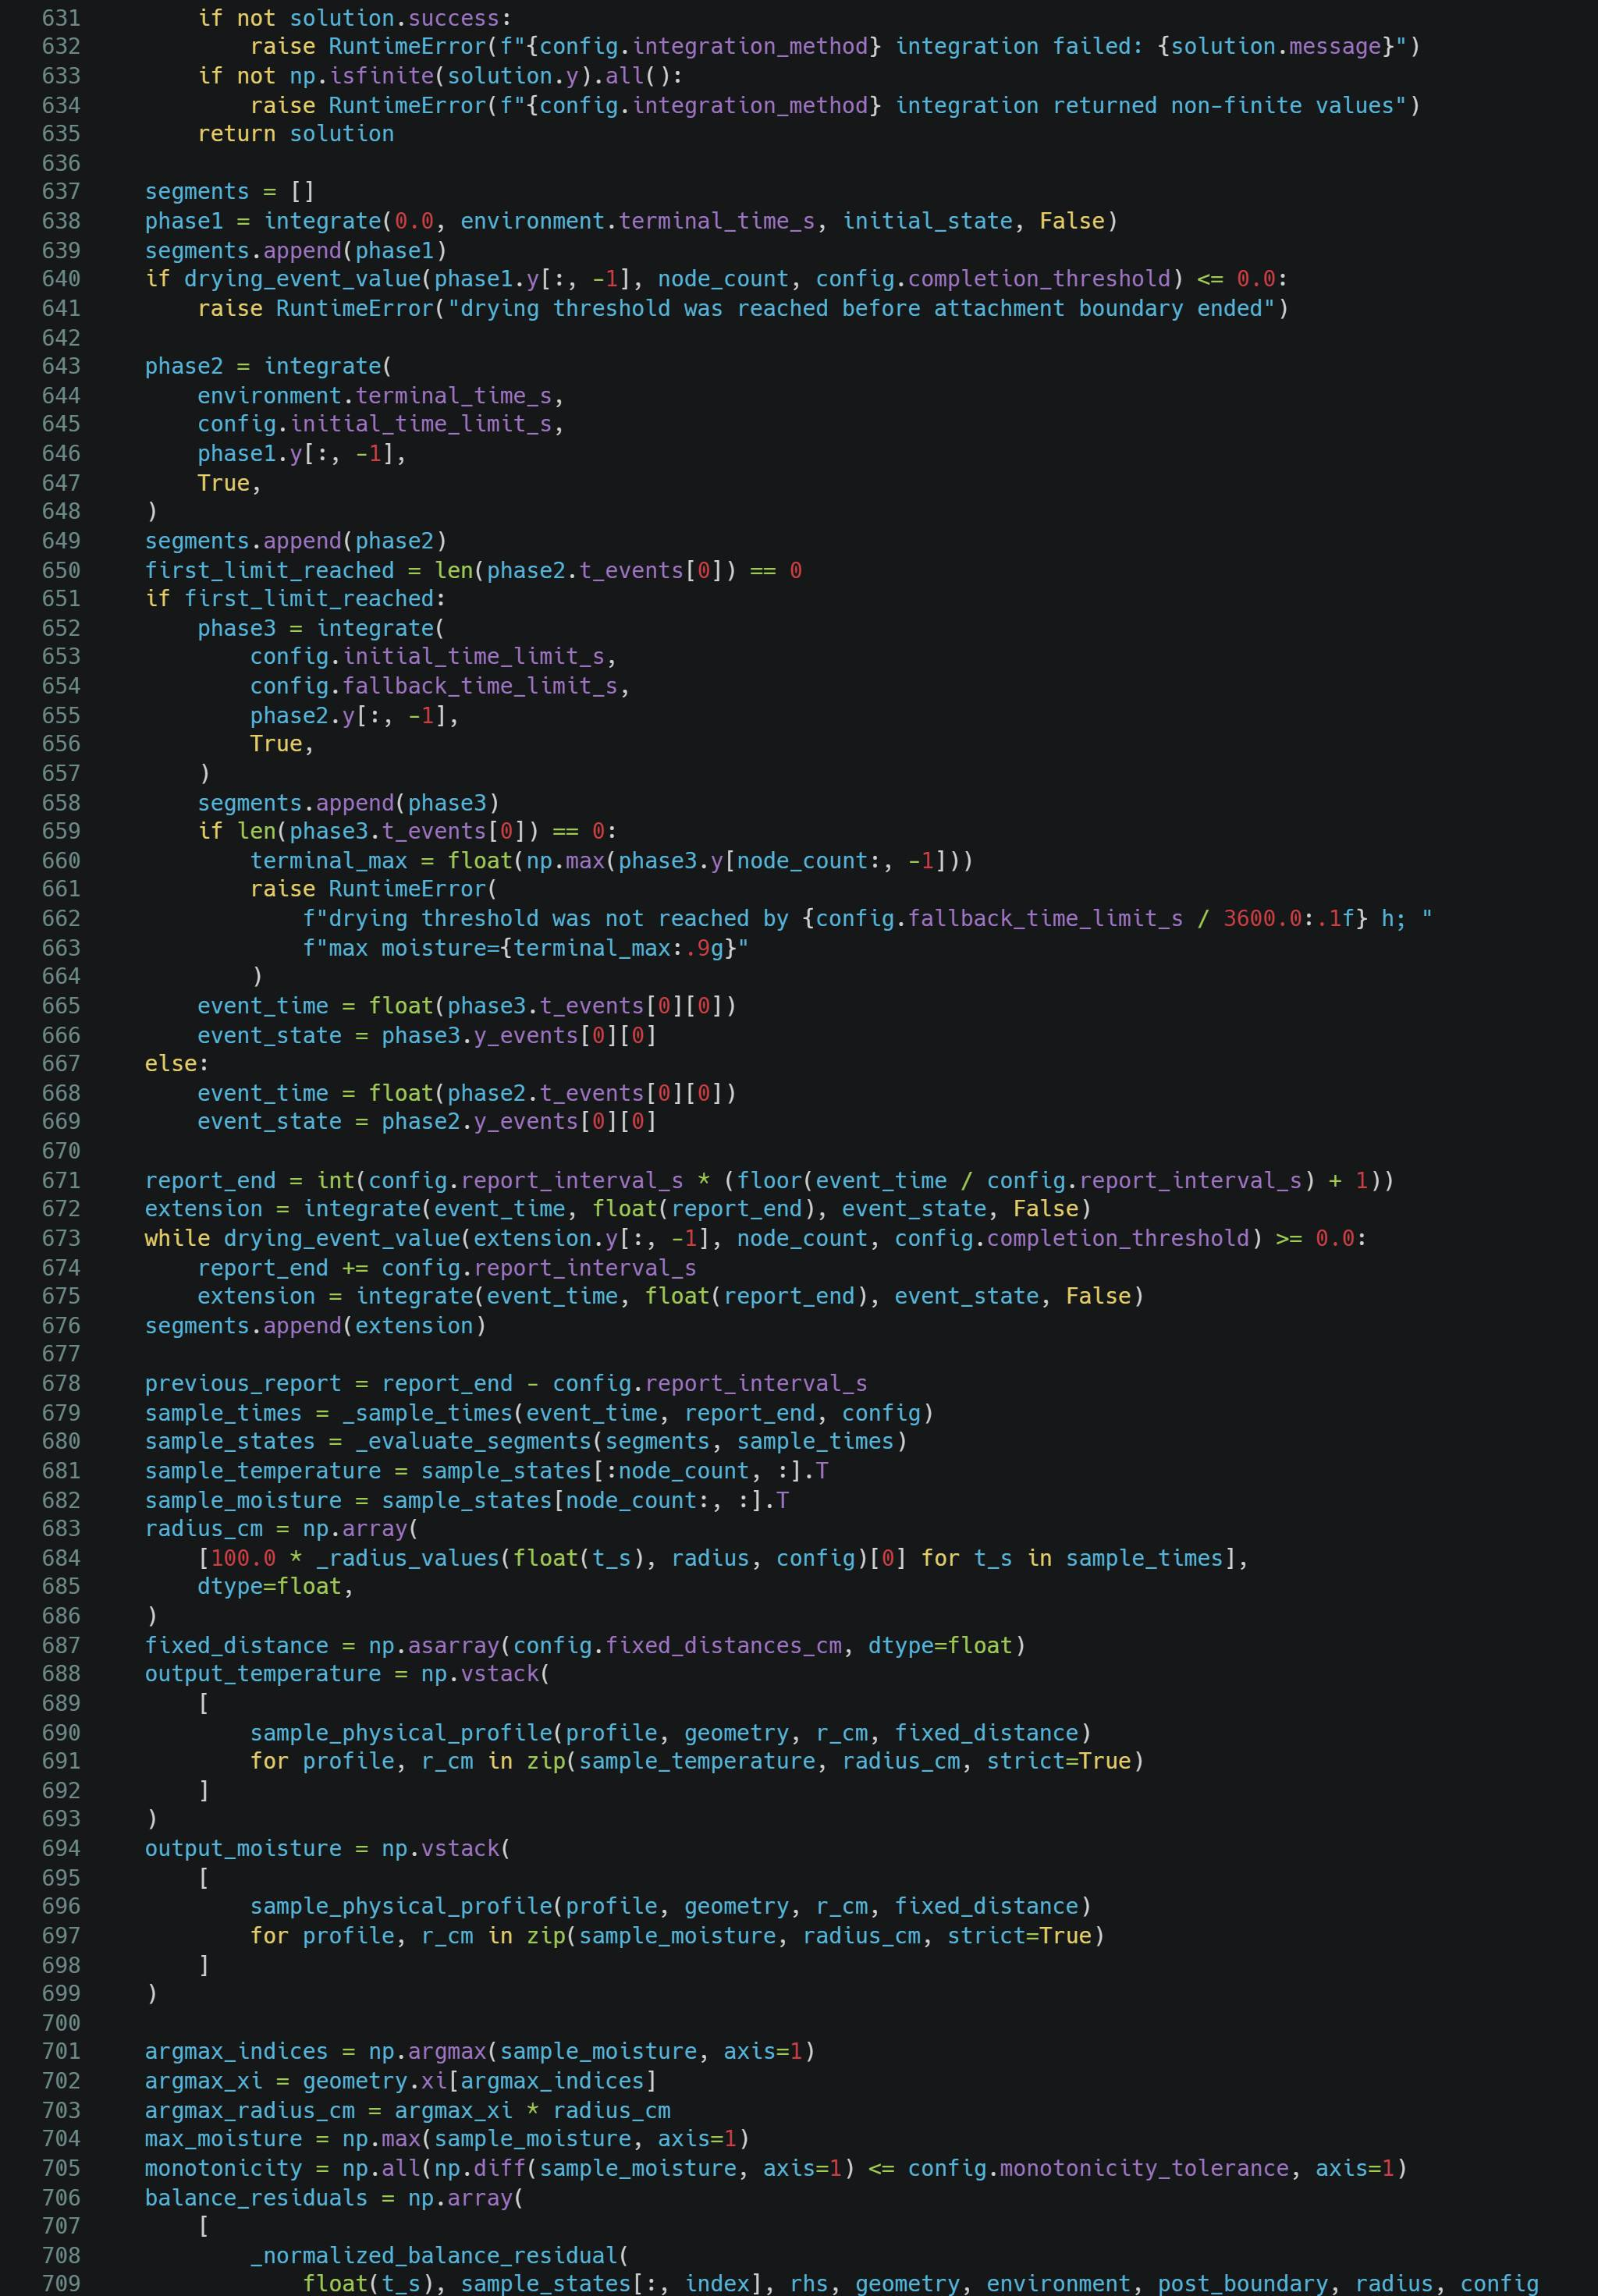
\includegraphics[width=\dimexpr\textwidth-24pt\relax]{../../code/submission/code_images/split/problem4_p9.jpg}
\newpage
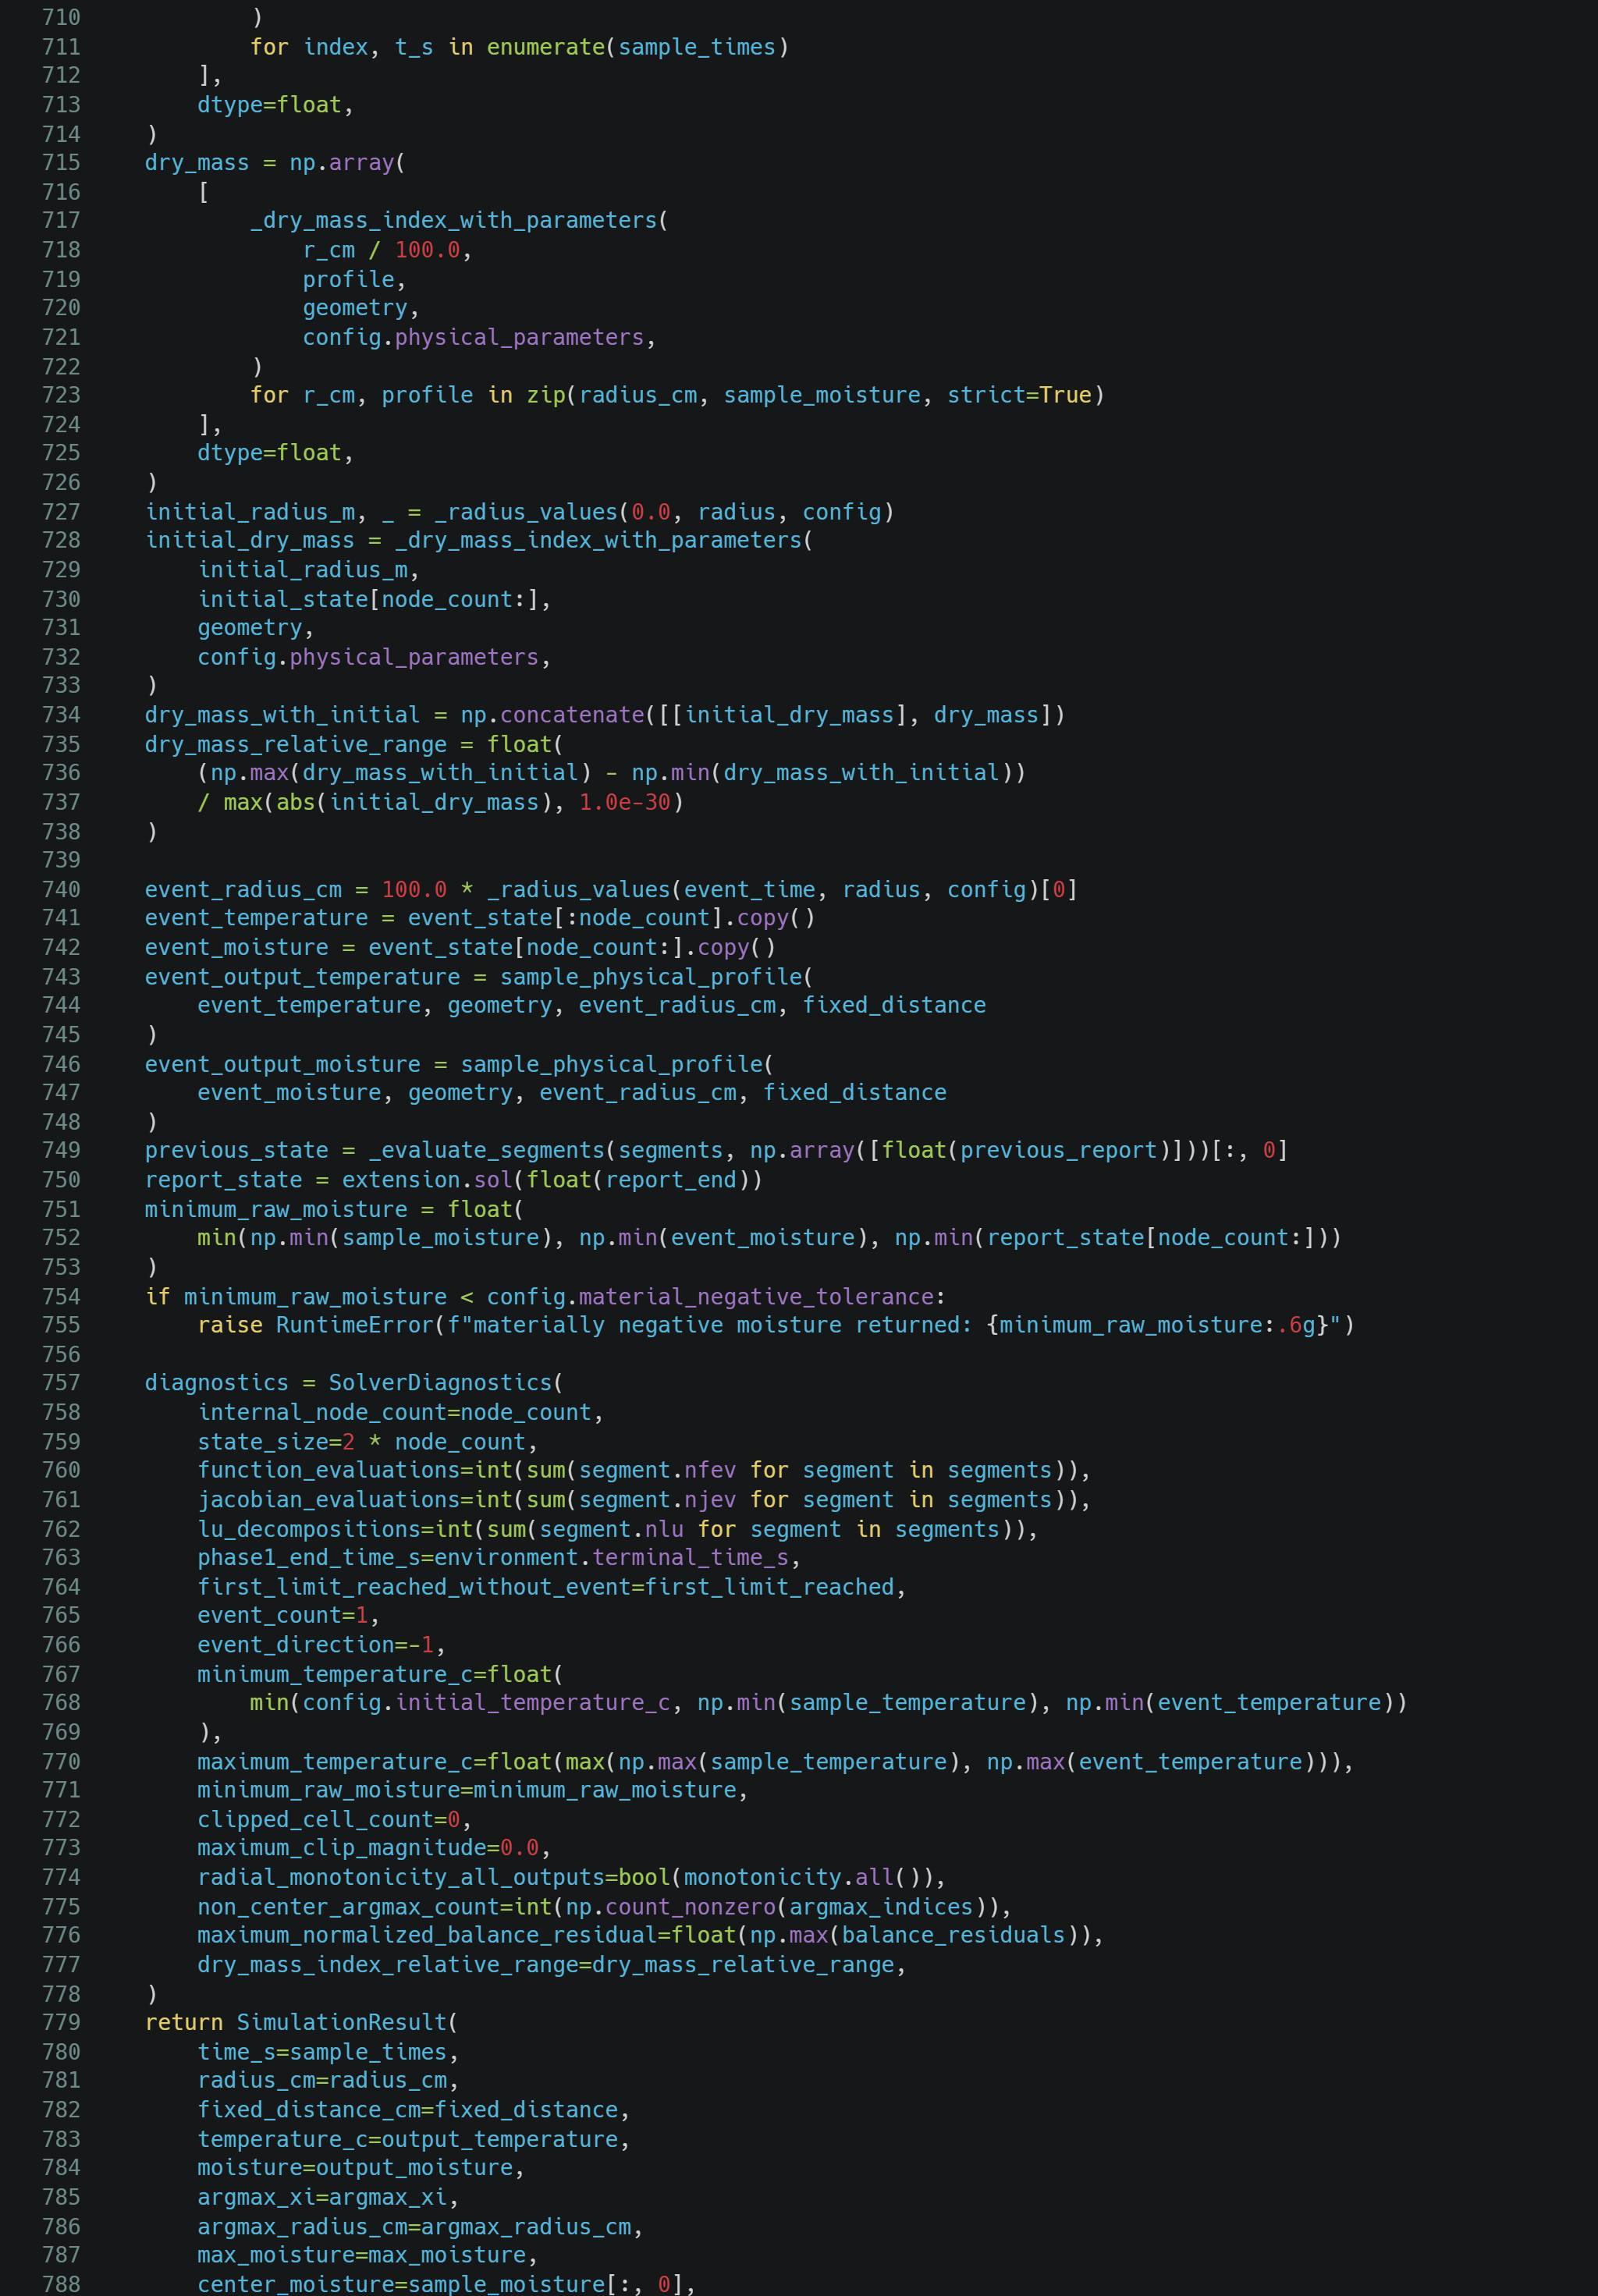
\includegraphics[width=\dimexpr\textwidth-24pt\relax]{../../code/submission/code_images/split/problem4_p10.jpg}
\newpage
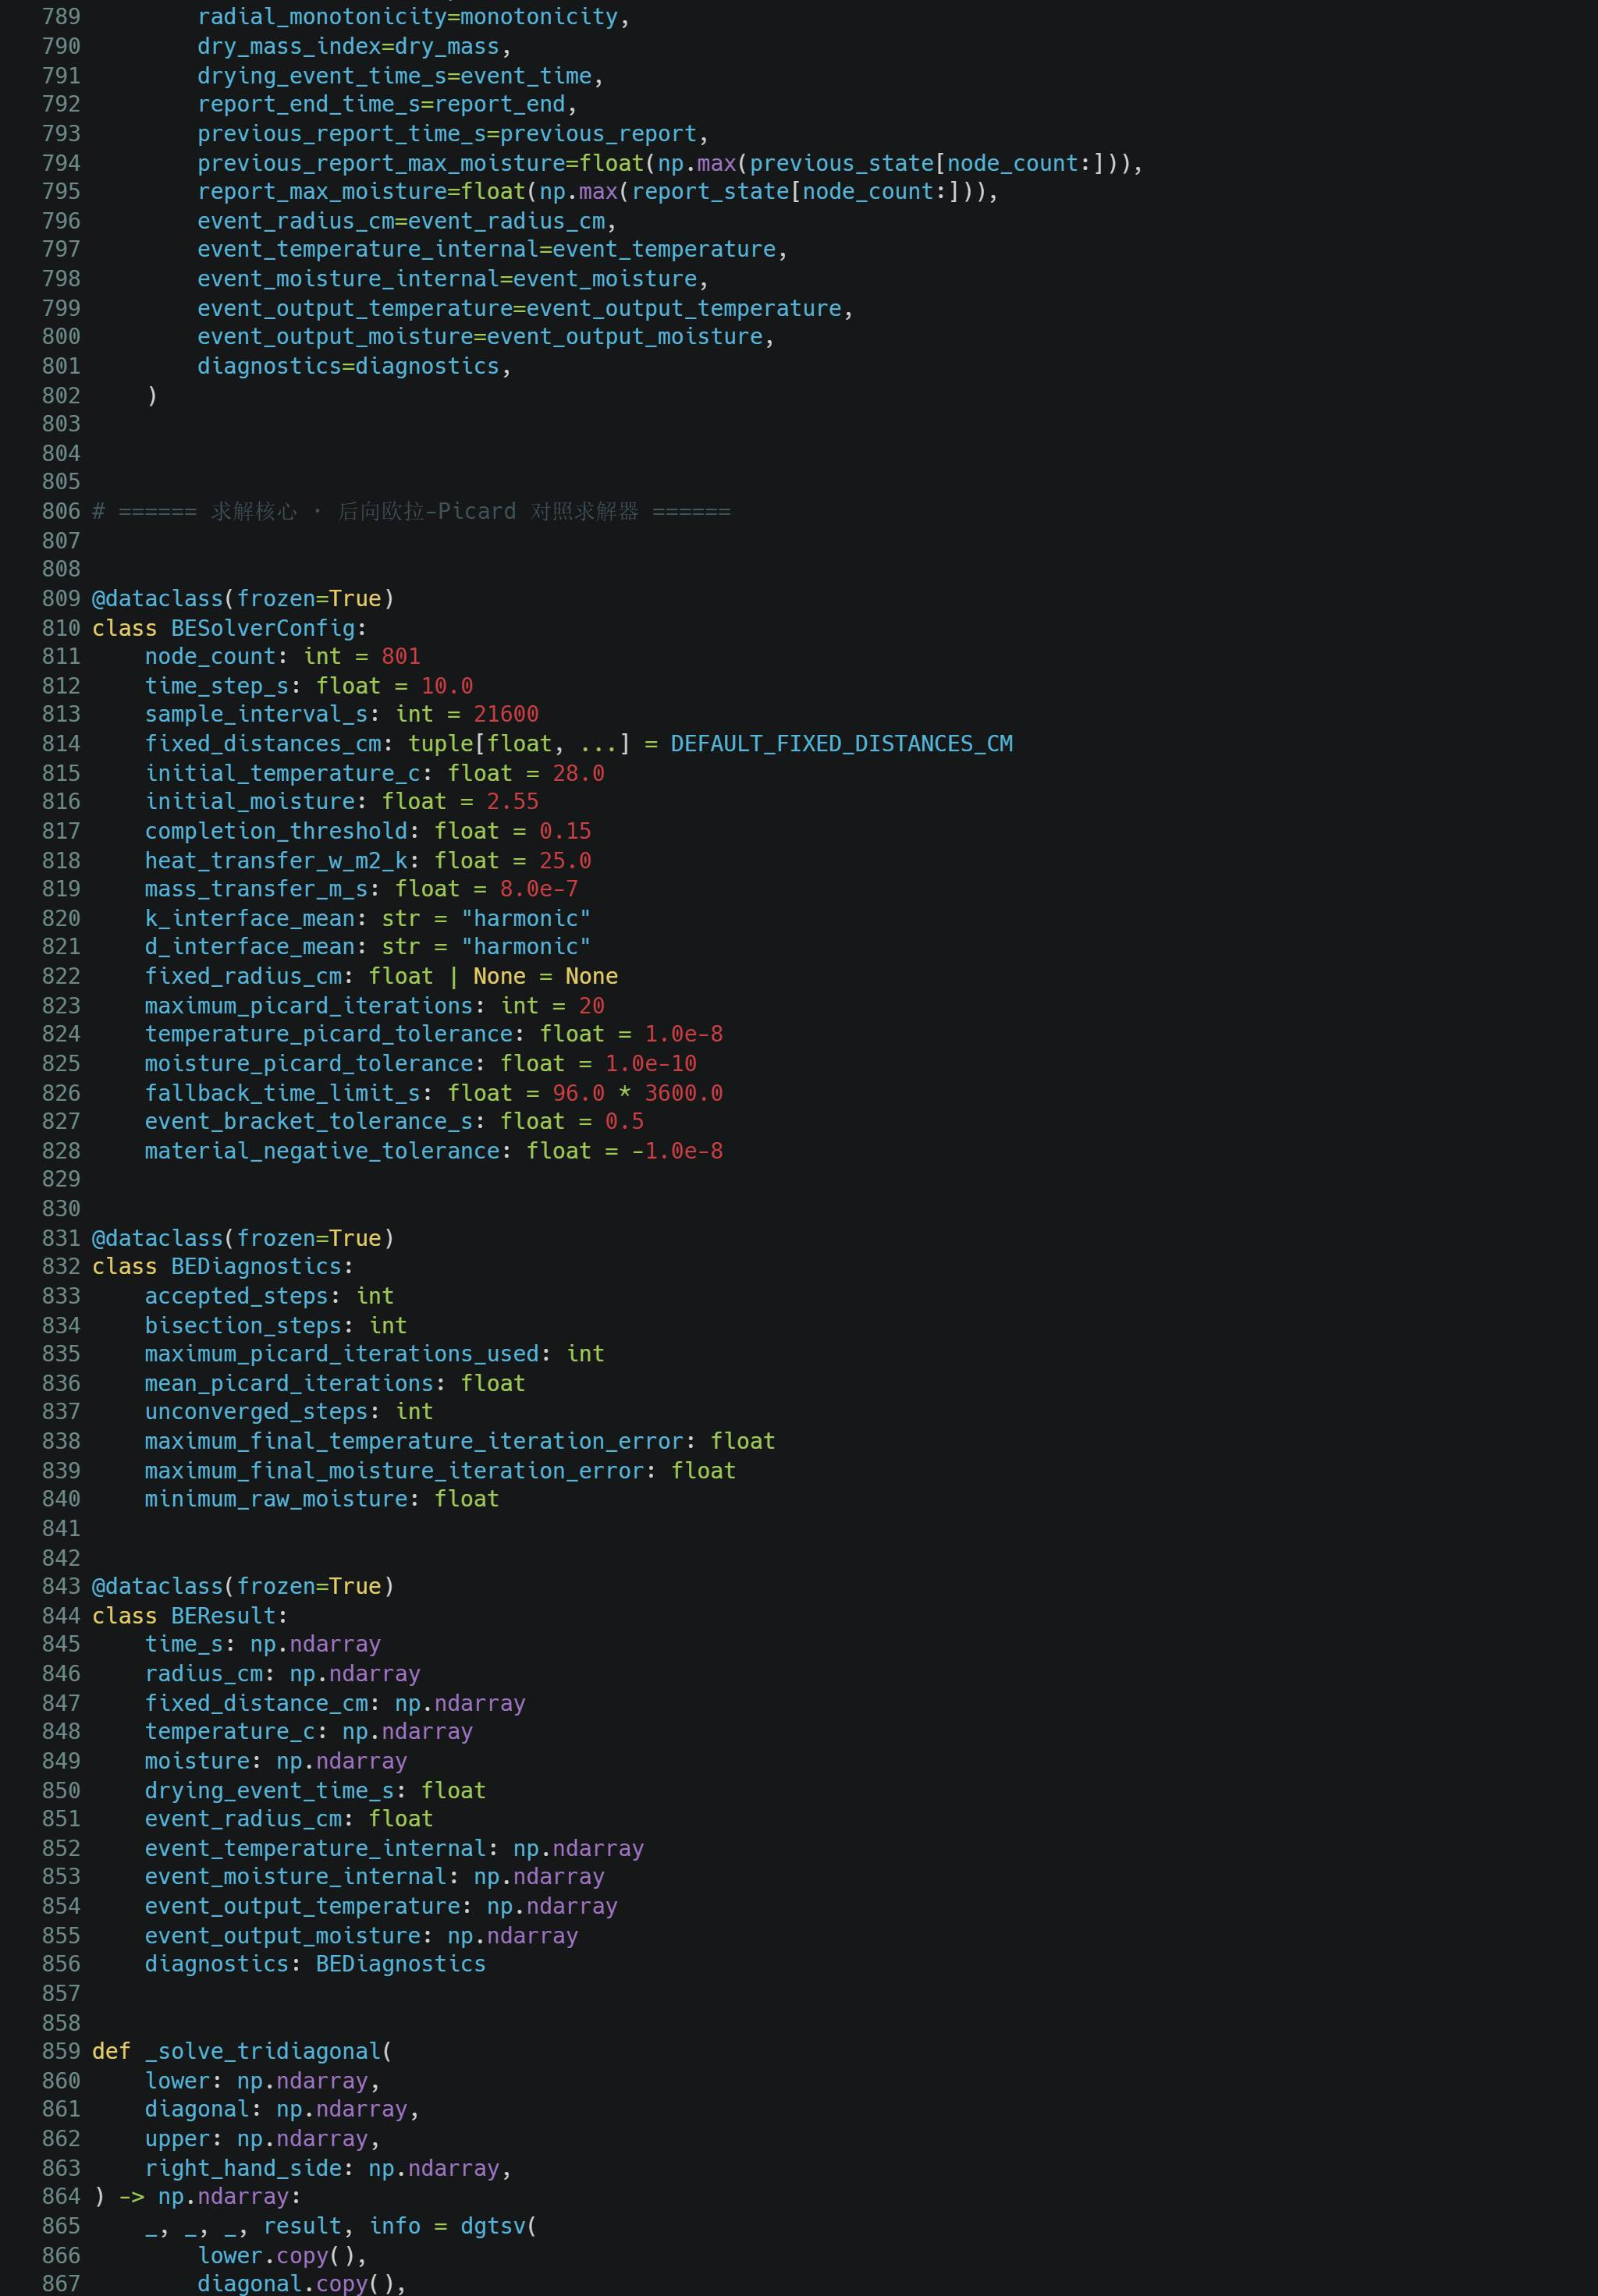
\includegraphics[width=\dimexpr\textwidth-24pt\relax]{../../code/submission/code_images/split/problem4_p11.jpg}
\newpage
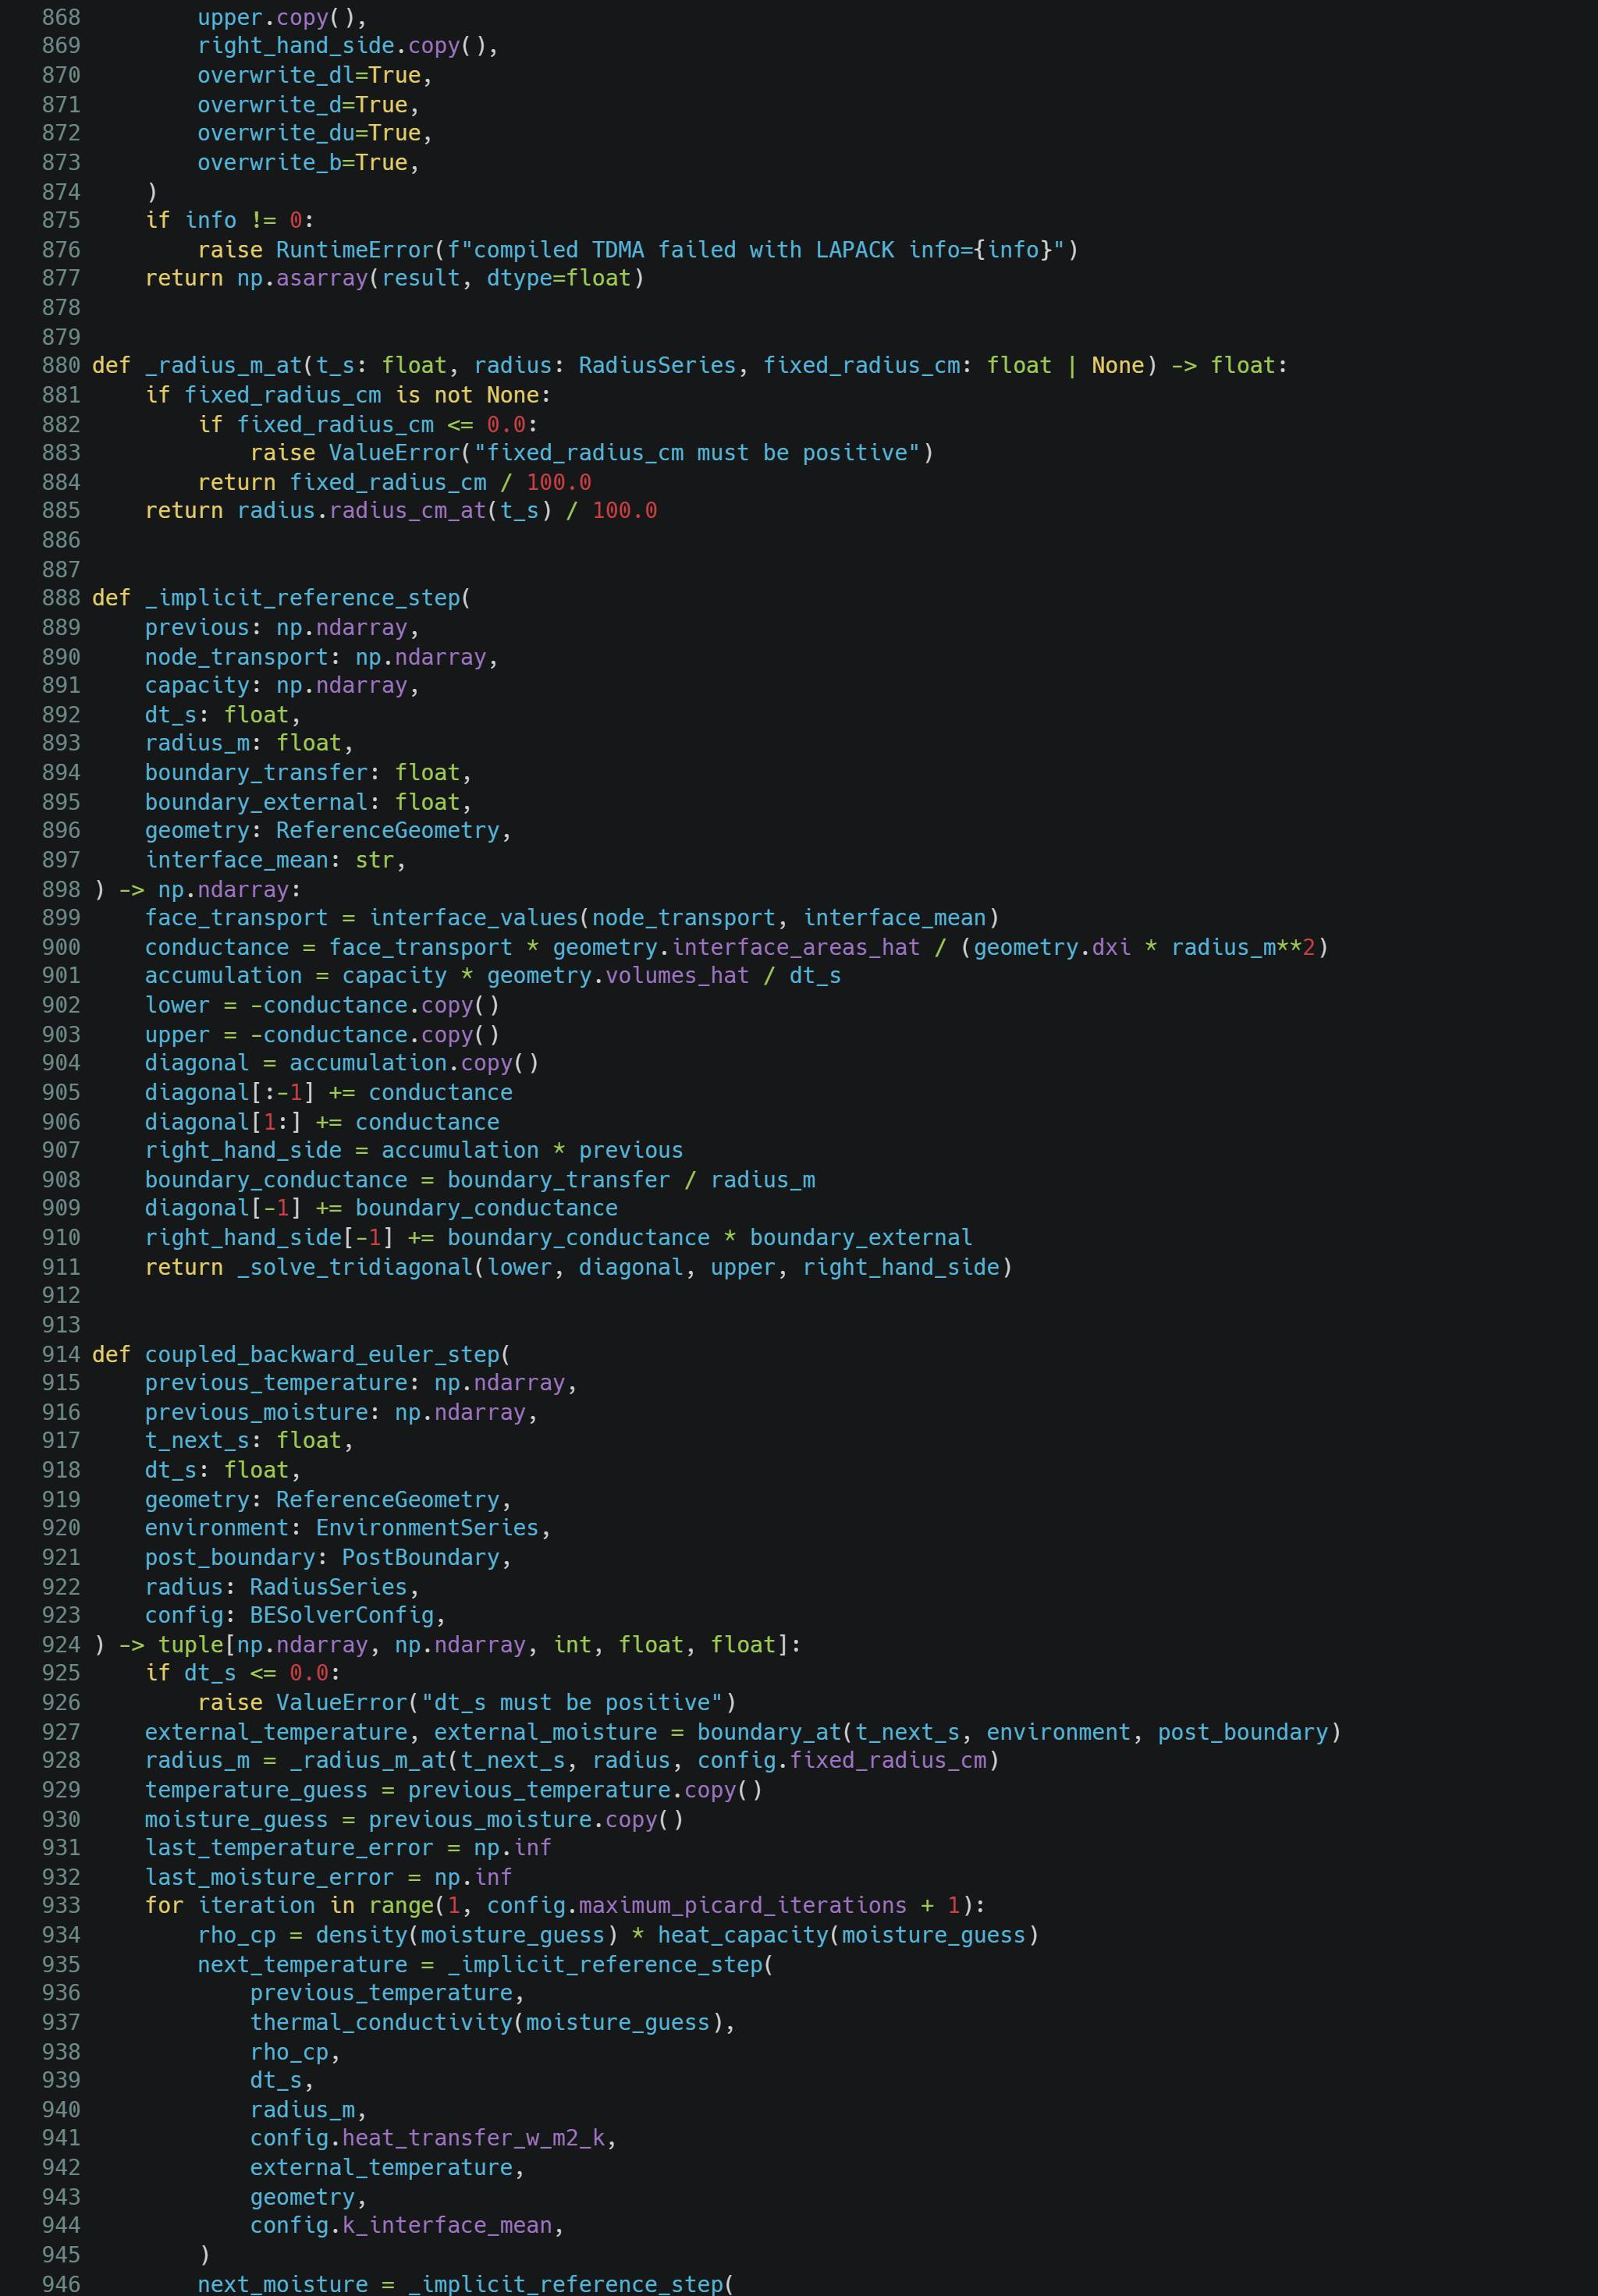
\includegraphics[width=\dimexpr\textwidth-24pt\relax]{../../code/submission/code_images/split/problem4_p12.jpg}
\newpage
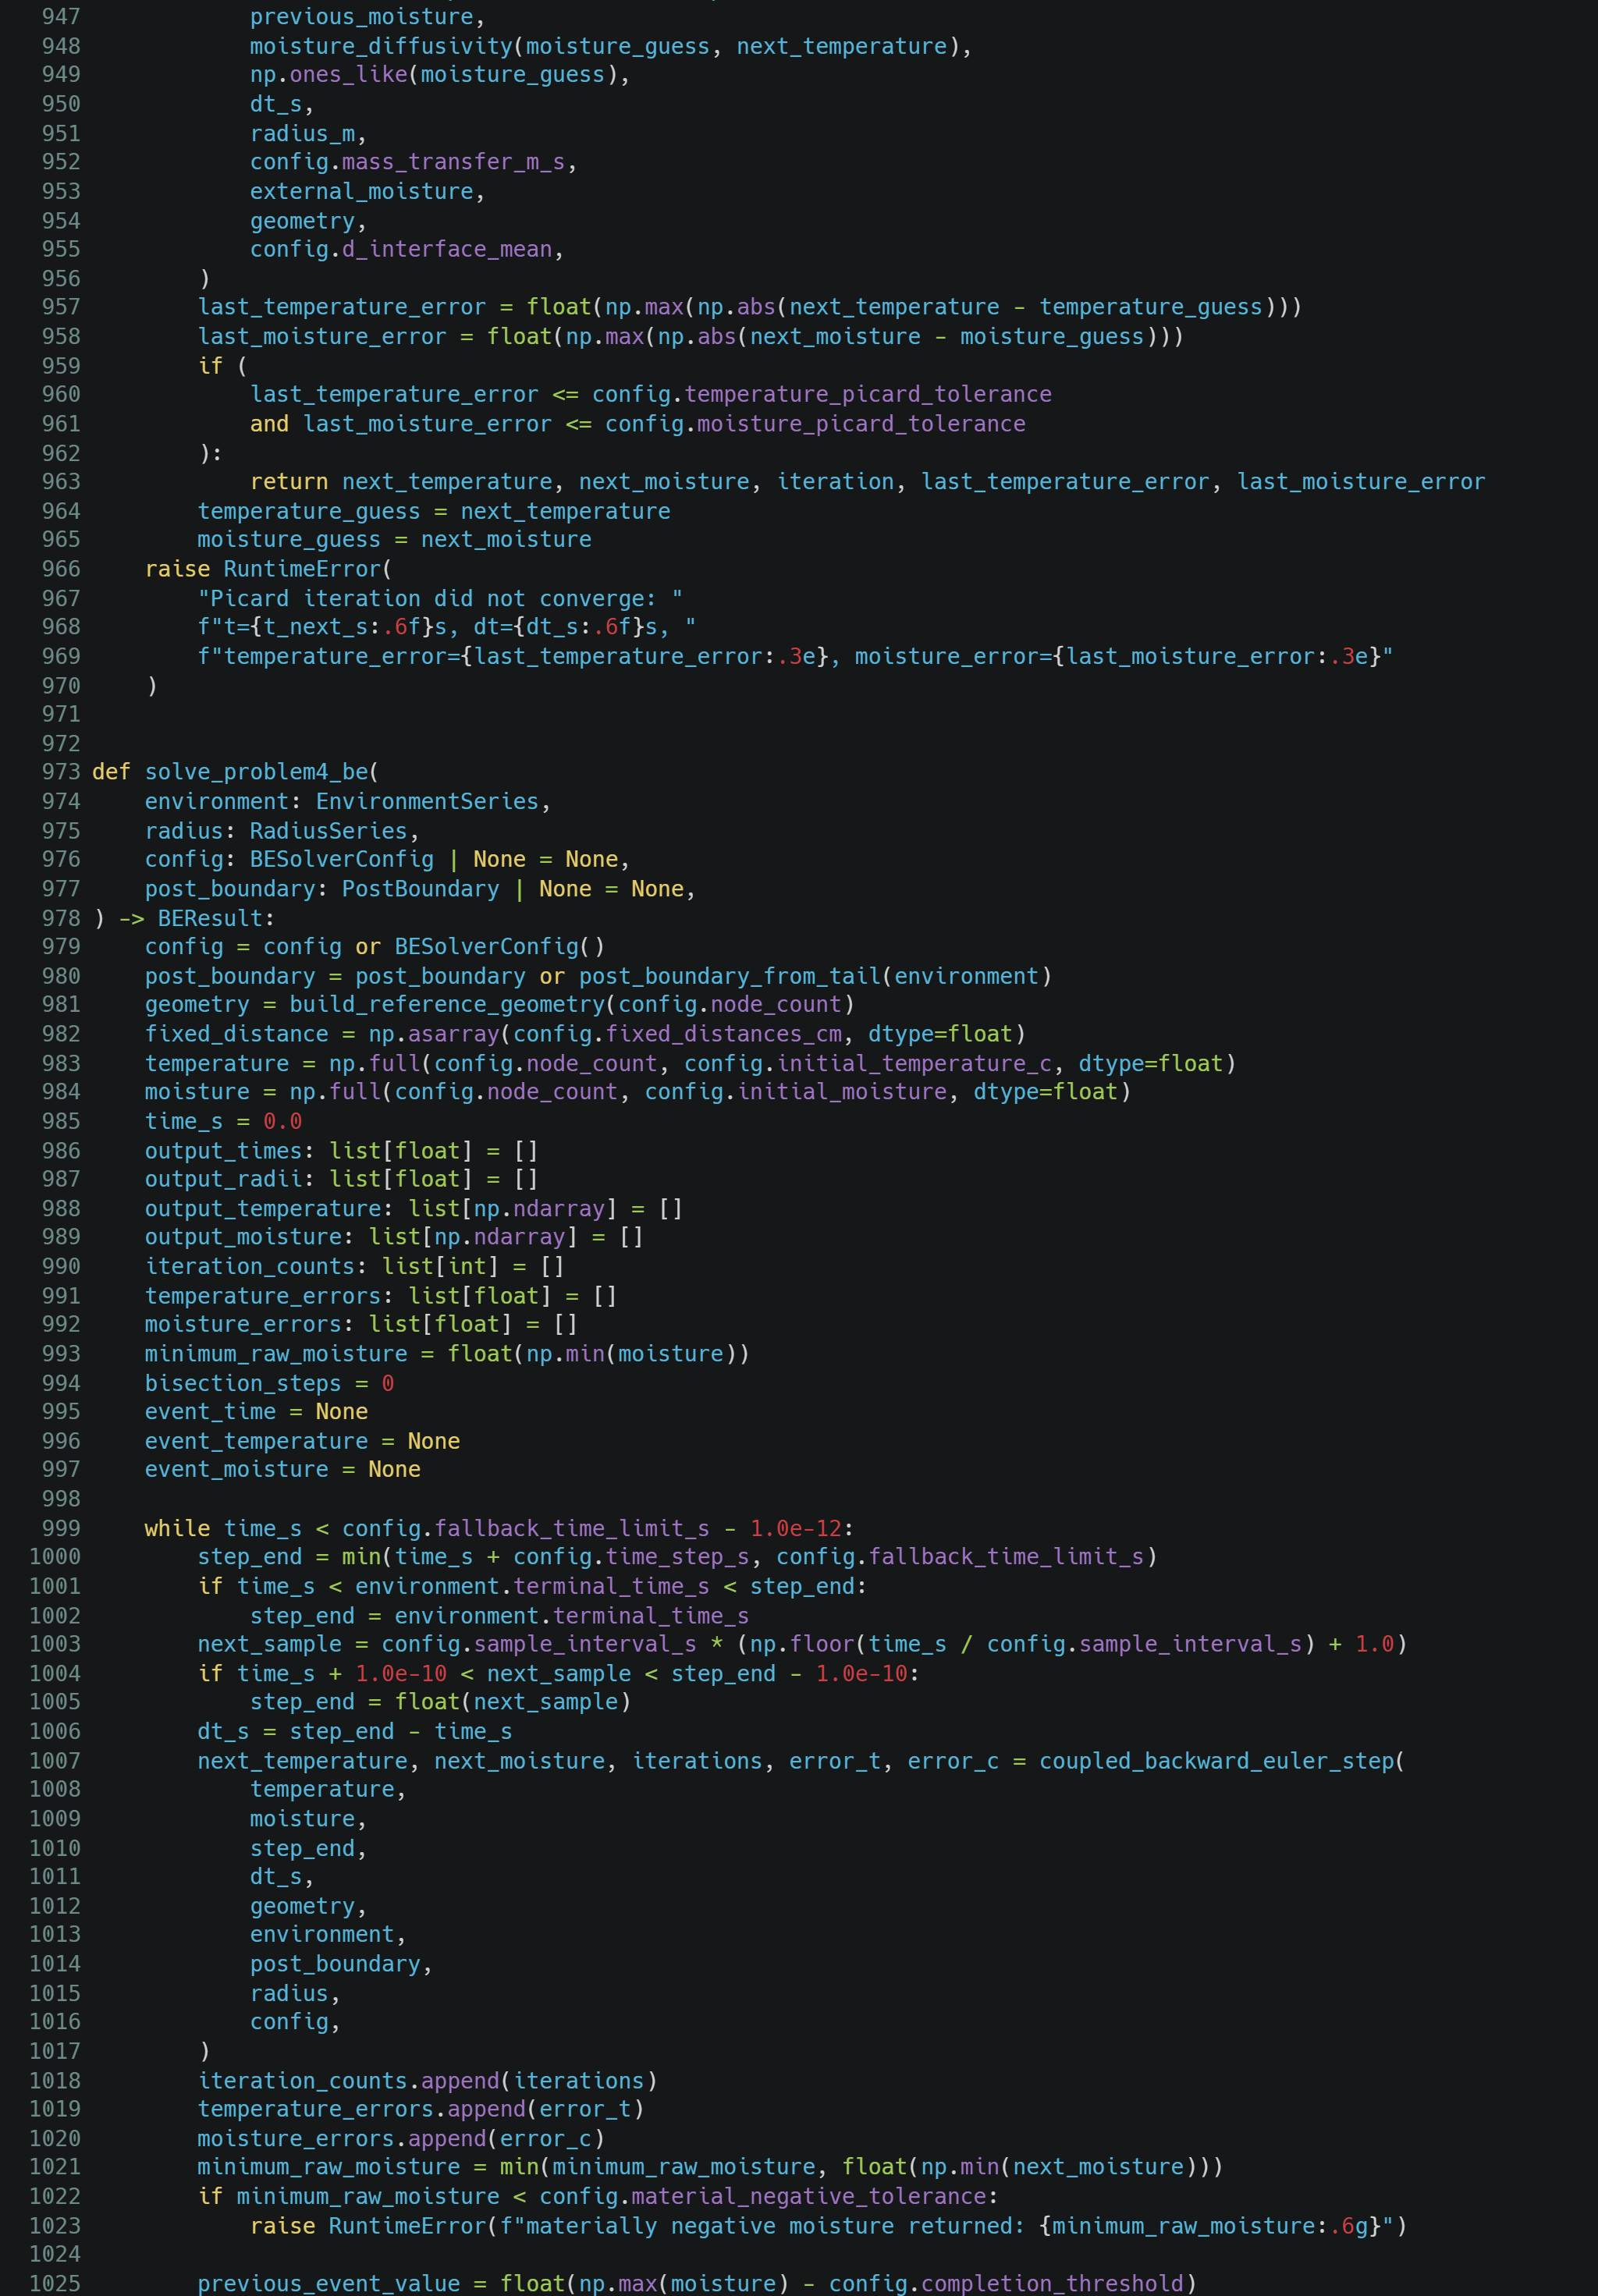
\includegraphics[width=\dimexpr\textwidth-24pt\relax]{../../code/submission/code_images/split/problem4_p13.jpg}
\newpage
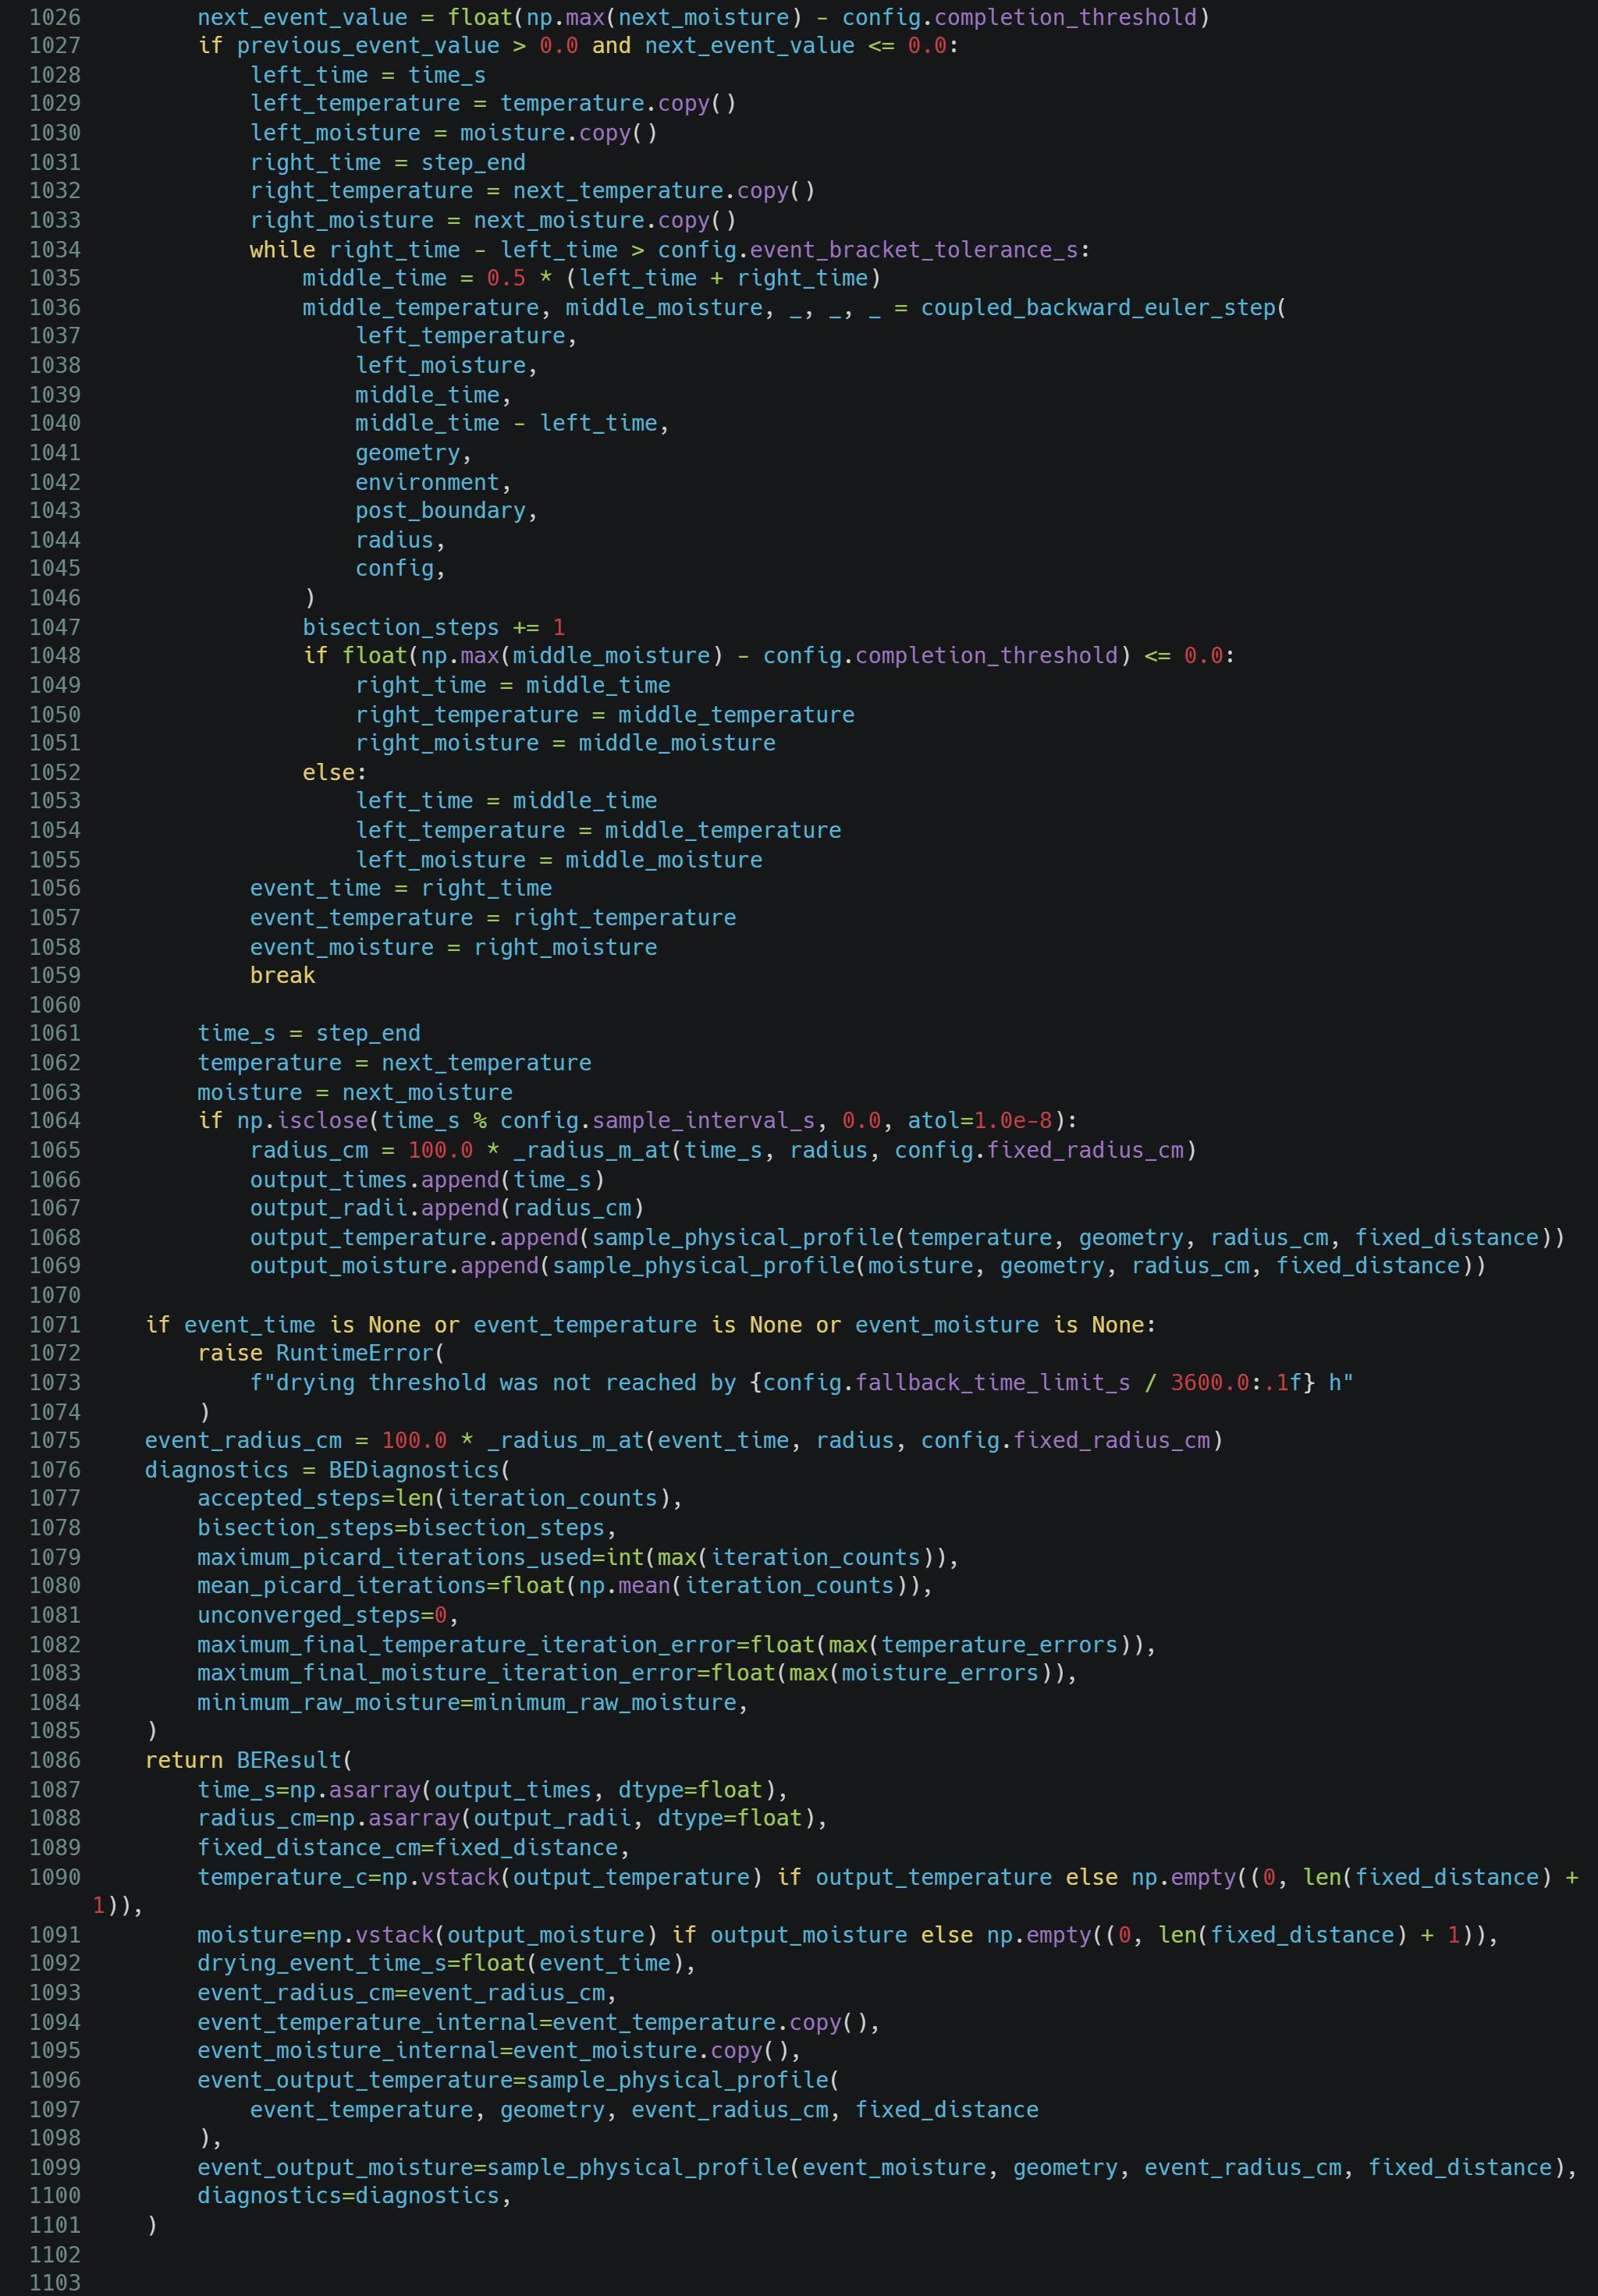
\includegraphics[width=\dimexpr\textwidth-24pt\relax]{../../code/submission/code_images/split/problem4_p14.jpg}
\newpage
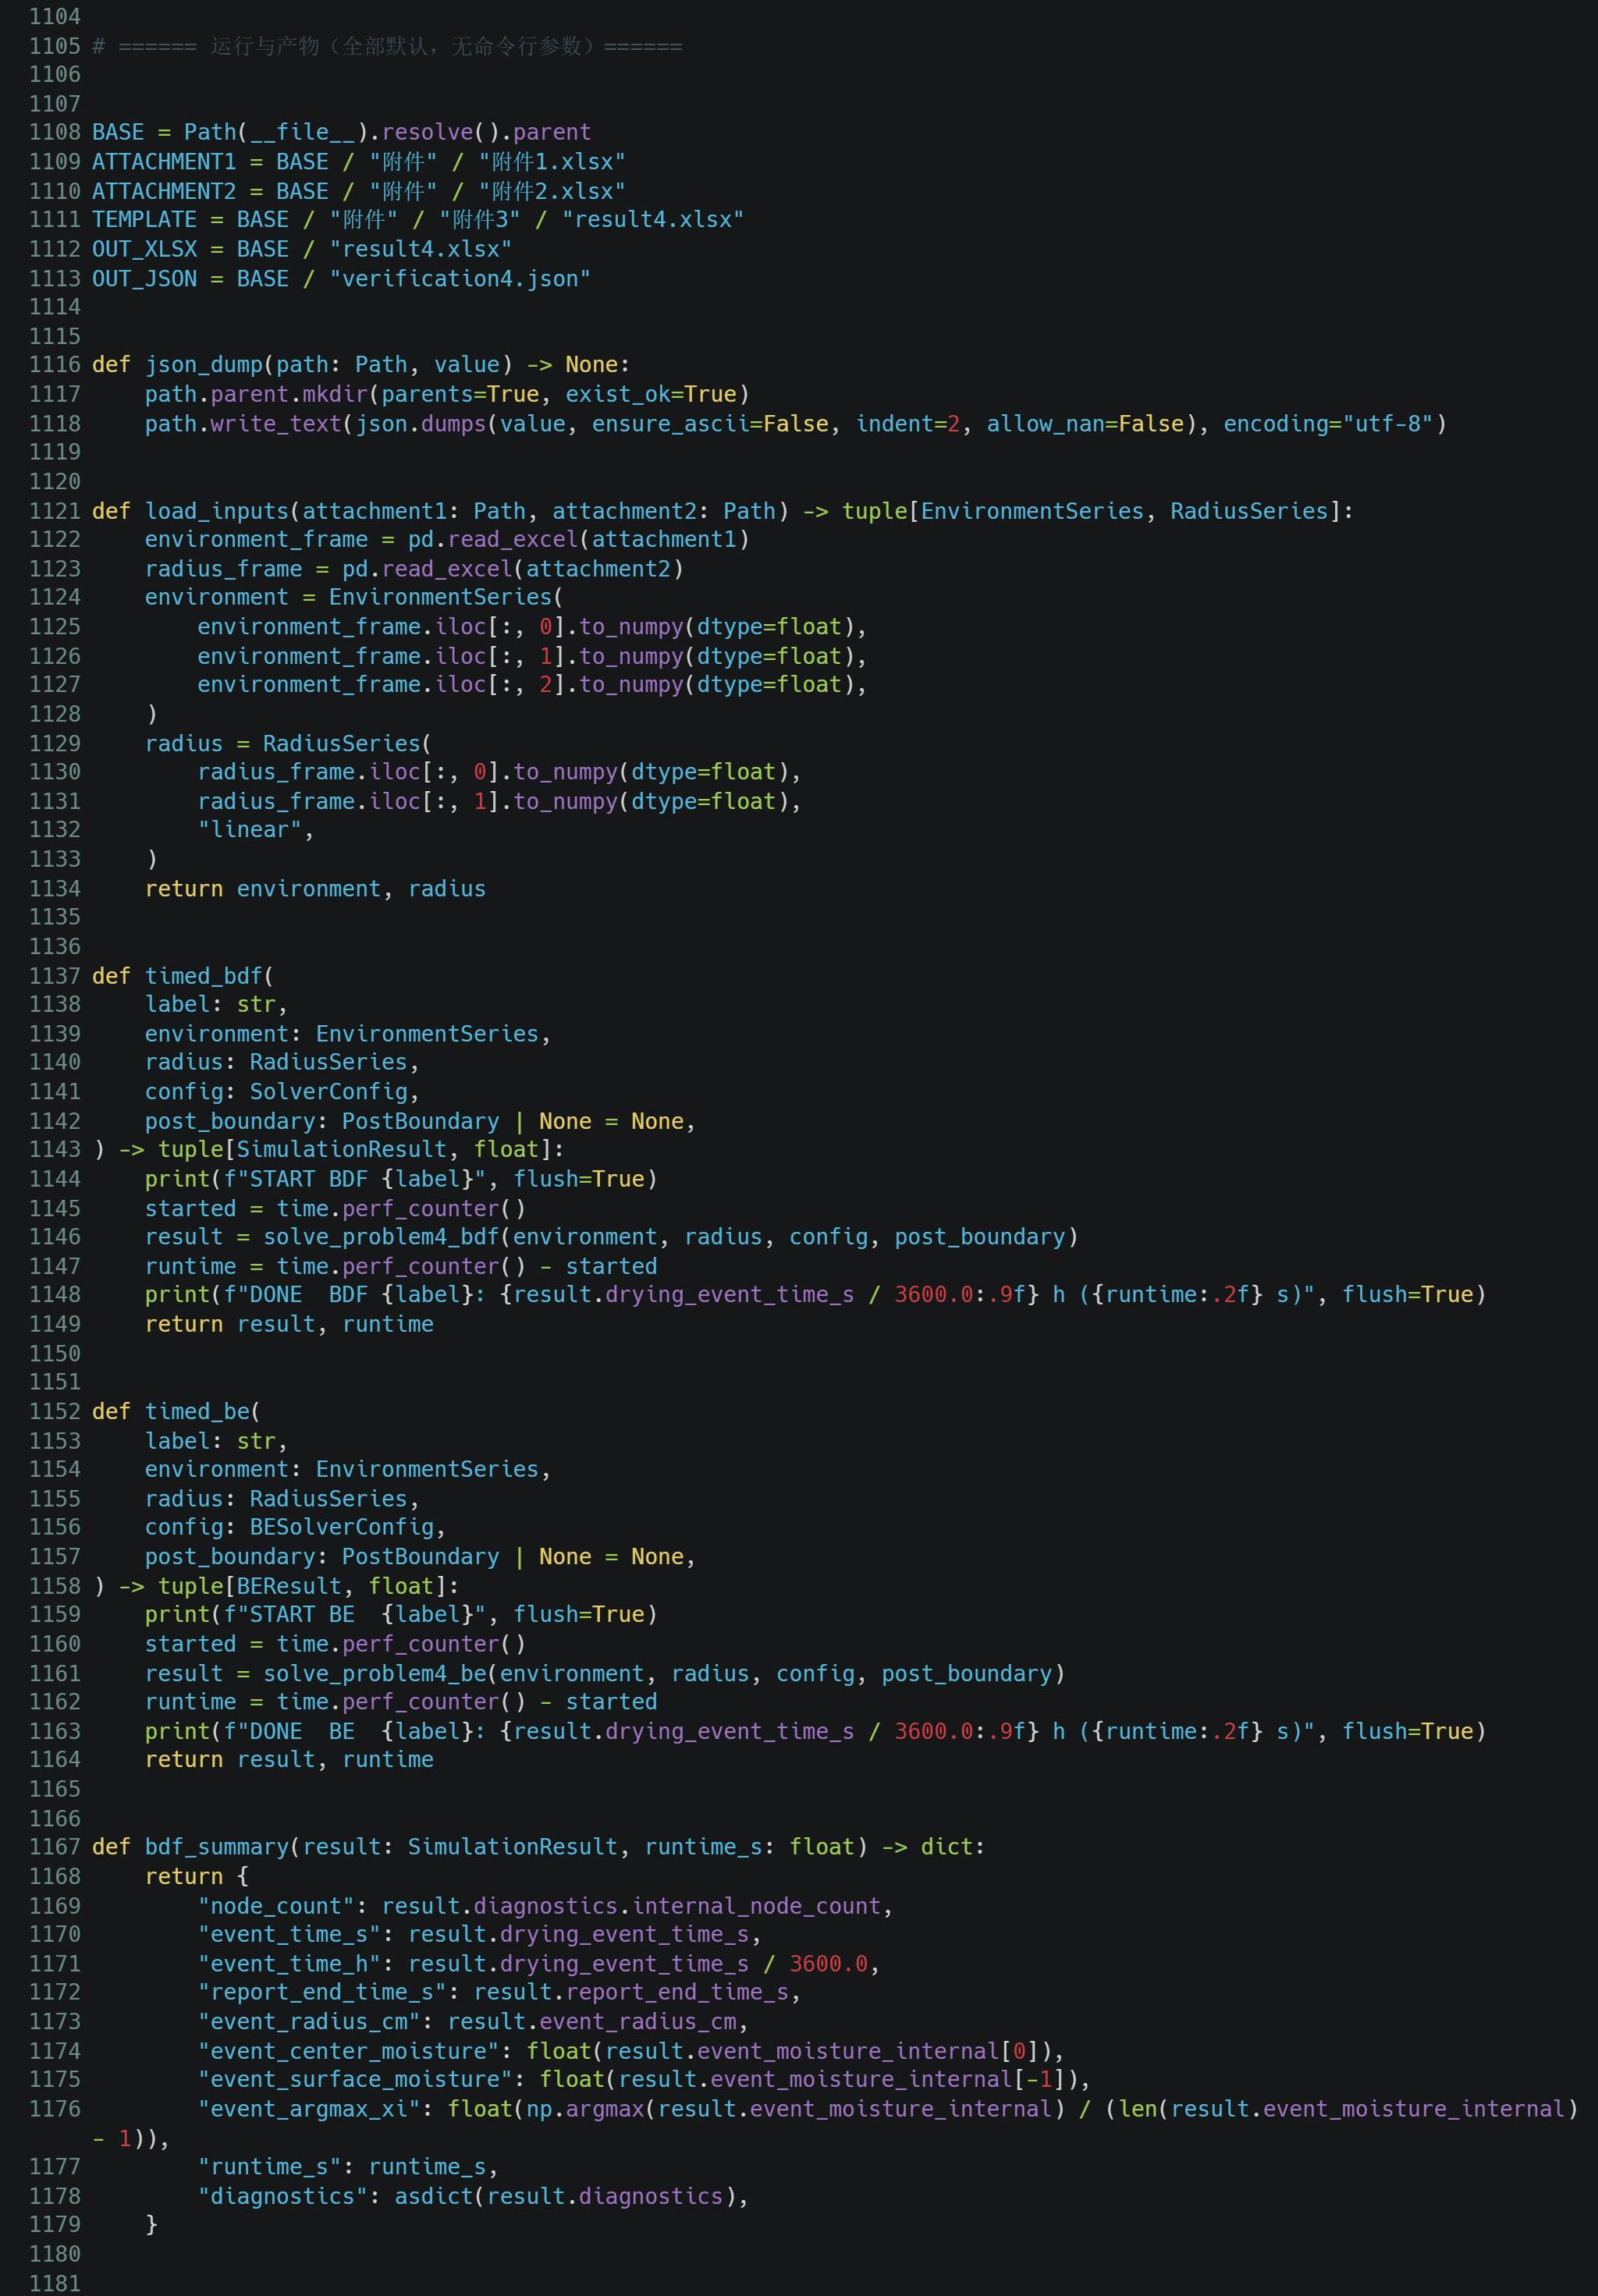
\includegraphics[width=\dimexpr\textwidth-24pt\relax]{../../code/submission/code_images/split/problem4_p15.jpg}
\newpage
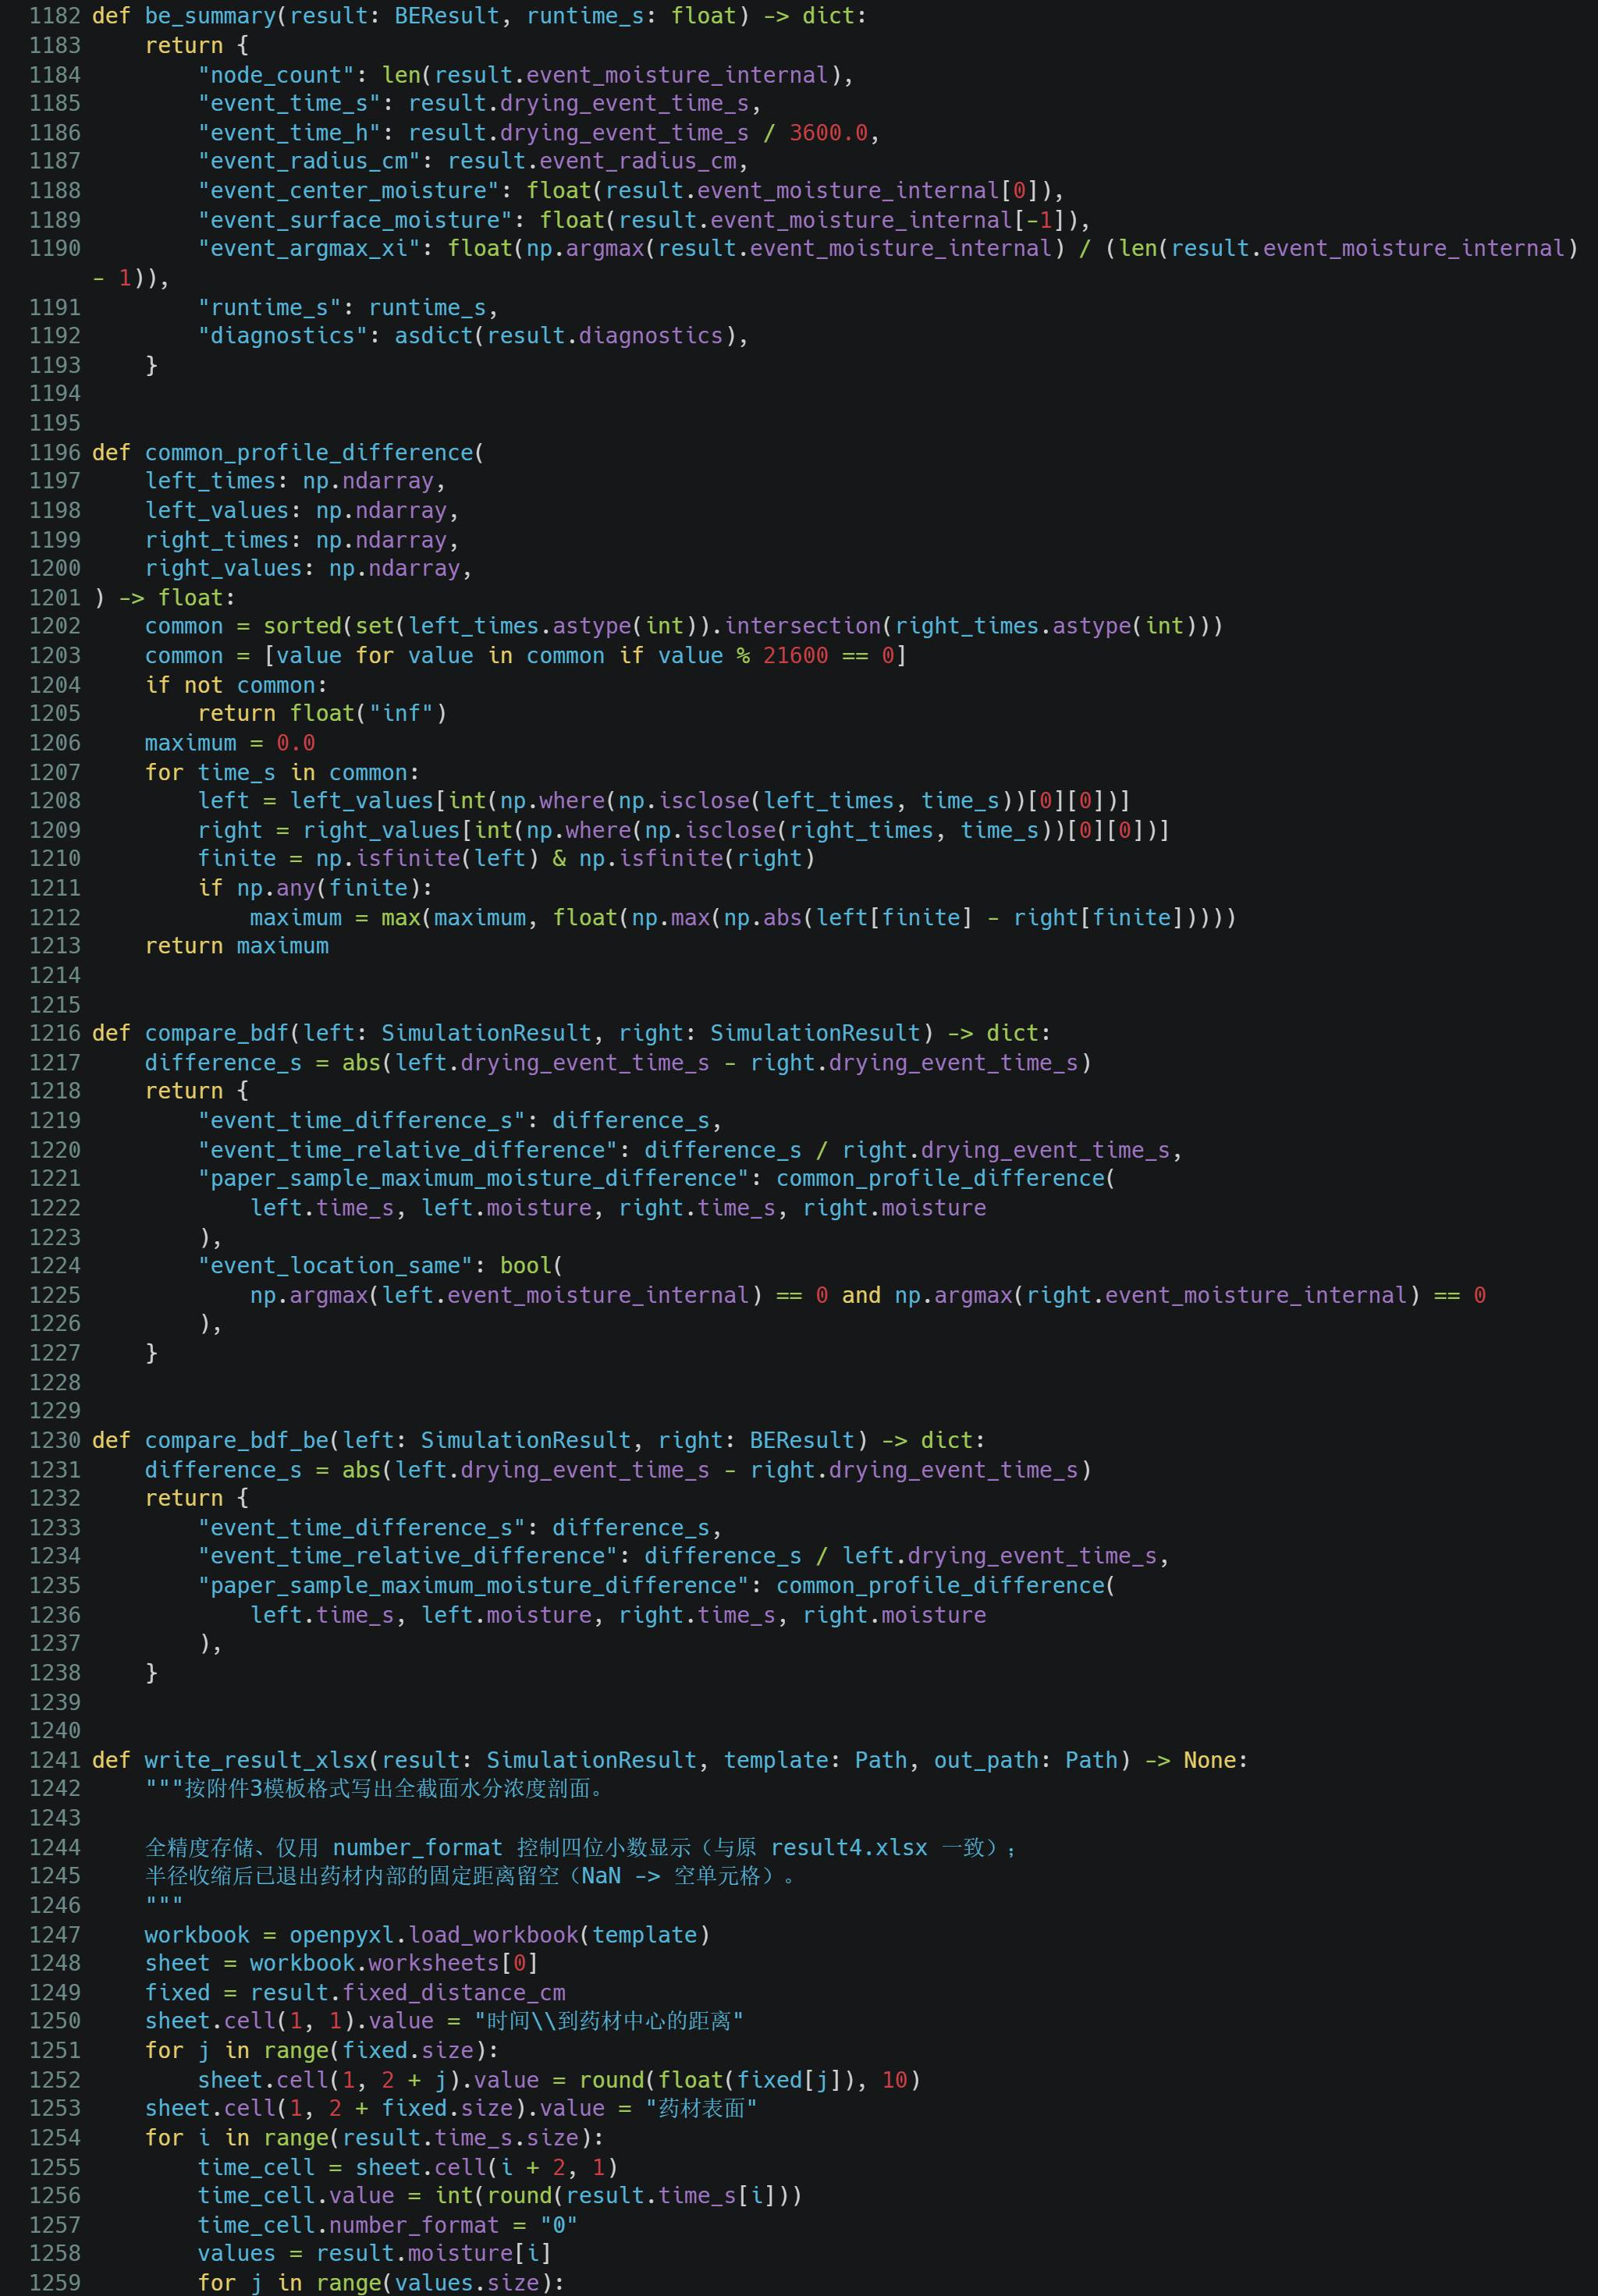
\includegraphics[width=\dimexpr\textwidth-24pt\relax]{../../code/submission/code_images/split/problem4_p16.jpg}

\end{document}
